%%%%%%%%%%%%%%%%%%%%%%%%%%%%%%%%%%%%%%%%%%%%%%%%%%%%%%%%%%%%%%%
%
%     filename  = "Cassie-Dissertation.tex",
%     version   = "1",
%     date      = "2017/02/10",
%     authors   = "Cassie N. Marker,
%     copyright = "Cassie N. Marker",
%     address   = "Materials Science and Engineering,
%                  319 Steidle Building,
%                  Penn State University,
%                  University Park, PA 16802,
%                  USA",
%     email     = "cnk118@psu.edu",
%
%%%%%%%%%%%%%%%%%%%%%%%%%%%%%%%%%%%%%%%%%%%%%%%%%%%%%%%%%%%%%%%
%
% Change History:
%
% 1.3.0	**	Added the cite package.
%
%		**	Give that the Graduate School now allows essentially
%			any line spacing, I have moved the line space setting
%			from psuthesis.cls to this driver file. Go ahead and
%			make it ugly if you want. :-)
%%%%%%%%%%%%%%%%%%%%%%%%%%%%%%%%%%%%%%%%%%%%%%%%%%%%%%%%%%%%%%%
%
% This is a template file to help get you started using the
% psuthesis.cls for theses and dissertations at Penn State
% University. You will, of course, need to put the
% psuthesis.cls file someplace that LaTeX will find it.
%
% We have set up a directory structure that we find to be clean
% and convenient. You can readjust it to suit your tastes. In
% fact, the structure used by our students is even a little
% more involved and commands are defined to point to the
% various directories.
%
% This document has been set up to be typeset using pdflatex.
% About the only thing you will need to change if typesetting
% using latex is the \DeclareGraphicsExtensions command.
%
% The psuthesis document class uses the same options as the
% book class. In addition, it requires that you have the
% ifthen, calc, setspace, and tocloft packages.
%
% The first additional option specifies the degree type. You
% can choose from:
%	Ph.D. using class option <phd>
%	M.S. using class option <ms>
%	M.Eng. using class option <meng>
%	M.A. using class option <ma>
%	B.S. using class option <bs>
%	B.A. using class option <ba>
%	Honors Baccalaureate using the option <honors>
%
% If you specify either ba or bs in addition to honors, it will
% just use the honors option and ignore the ba or bs option.
%
% The second additional option <inlinechaptertoc> determines
% the formatting of the Chapter entries in the Table of
% Contents. The default sets them as two-line entries (try it).
% If you want them as one-line entries, issue the
% inlinechaptertoc option.
%
% The class option ``honors'' should be used for theses
% submitted to the Schreyer Honors College. This option
% changes the formatting on the Title page so that the
% signatures appear on the Title page.
%
% The class option ``honorsdepthead'' adds the signature of the
% department head on the Title page for those baccalaureate
% theses that require this.
%
% The class option ``secondthesissupervisor'' should be used
% for baccalaureate honors degrees if you have a second
% Thesis Supervisor.
%
% The vita is only included with the phd option and it is
% placed at the end of the thesis. The permissions page is only
% included with the ms, meng, and ma options.
%%%%%%%%%%%%%%%%%%%%%%%%%%%%%%%%%%%%%%%%%%%%%%%%%%%%%%%%%%%%%%%
\documentclass[phd,12pt]{psuthesis}

\usepackage[T1]{fontenc}
\usepackage{lmodern}
\usepackage{textcomp}
\usepackage{microtype}

%%%%%%%%%%%%%%%%%%%%%%%%%%%%
% Packages we like to use. %
%%%%%%%%%%%%%%%%%%%%%%%%%%%%
\usepackage{amsmath}
\usepackage{amssymb}
\usepackage{amsthm}
\usepackage{exscale}
\usepackage[mathscr]{eucal}
\usepackage{bm}
\usepackage{eqlist} % Makes for a nice list of symbols.
\usepackage[final]{graphicx}
\usepackage[dvipsnames]{color}
\DeclareGraphicsExtensions{.pdf, .jpg}
\usepackage{float}
\usepackage{gensymb}
\usepackage{longtable}
\usepackage{caption}
\usepackage{wasysym}
% http://www.tex.ac.uk/cgi-bin/texfaq2html?label=citesort
\usepackage{cite}

\usepackage{titlesec}

%%%%%%%%%%%%%%%%%%%%%%%%%%%%%%%
% Use of the hyperref package %
%%%%%%%%%%%%%%%%%%%%%%%%%%%%%%%
%
% This is optional and is included only for those students
% who want to use it.
%
% To the hyperref package, uncomment the following line:
\usepackage{hyperref}
%
% Note that you should also uncomment the following line:
\renewcommand{\theHchapter}{\thepart.\thechapter}
%
% to work around some a problem hyperref has with the fact
% the psuthesis class has unnumbered pages after which page
% counters are reset.

% Set the baselinestretch using the setspace package.
% The LaTeX Companion claims that a \baselinestretch of
% 1.24 gives one-and-a-half line spacing, which is allowed
% by the PSU thesis office. As of October 18, 2013, the Graduate
% School states ``The text of an eTD may be single-, double- or
% one- and-a-half-spaced.'' Go nuts!
\setstretch{1.24}


%%%%%%%%%%%%%%%%%%%%%%%%%%%%%%%%%%%%
% SPECIAL SYMBOLS AND NEW COMMANDS %
%%%%%%%%%%%%%%%%%%%%%%%%%%%%%%%%%%%%
% Place user-defined commands below.



%%%%%%%%%%%%%%%%%%%%%%%%%%%%%%%%%%%%%%%%%
% Renewed Float Parameters              %
% (Makes floats fit better on the page) %
%%%%%%%%%%%%%%%%%%%%%%%%%%%%%%%%%%%%%%%%%
\renewcommand{\floatpagefraction}{0.85}
\renewcommand{\topfraction}      {0.85}
\renewcommand{\bottomfraction}   {0.85}
\renewcommand{\textfraction}     {0.15}

% ----------------------------------------------------------- %

%%%%%%%%%%%%%%%%
% FRONT-MATTER %
%%%%%%%%%%%%%%%%
% Title
\title{DEVELOPMENT OF A KNOWLEDGE BASE OF TI-ALLOYS FROM FIRST-PRINCIPLES AND COMPUTATIONAL THERMODYNAMICS}

% Author and Department
\author{Cassie Marker}
\dept{Materials Science and Engineering}
% the degree will be conferred on this date
\degreedate{August 2017}
% year of your copyright
\copyrightyear{2017}


% This is the document type. For example, this could also be:
%	Comprehensive Document
%	Thesis Proposal
%\documenttype{Thesis}
\documenttype{Dissertation}
%\documenttype{Comprehensive Document}


% This will generally be The Graduate School, though you can
% put anything in here to suit your needs.
\submittedto{The Graduate School}

% This is the college to in which you are submitting the
% thesis/dissertation.
\collegesubmittedto{College of Earth and Mineral Sciences}


%%%%%%%%%%%%%%%%%%
% Signatory Page %
%%%%%%%%%%%%%%%%%%
% You can have up to 7 committee members, i.e., one advisor
% and up to 6 readers.
%
% Begin by specifying the number of readers.
\numberofreaders{4}

% Input reader information below. The optional argument, which
% comes first, goes on the second line before the name.
\advisor[Thesis Advisor, Chair of Committee]
		{Zi-Kui Liu}
		{Professor of Materials Science and Engineering}

\readerone
			{Allison Beese}
			{Assistant Professor of Materials Science and Engineering}

\readertwo
			{Kristen Fichthorn}
			{Merrell Fenskey Professor of Chemical Engineering and Professor of Physics}

\readerthree[Special Member]
			{Michael Manley}
			{Senior Researcher, Oak Ridge National Laboratory, Materials Science \& Technology Division}

\readerfour
			{Susan Sinnott}
			{Department Head and Professor of Materials Science and Engineering}

% Format the Chapter headings using the titlesec package.
% You can format section headings and the like here too.
\definecolor{gray75}{gray}{0.75}
\newcommand{\hsp}{\hspace{15pt}}
\newcommand{\hourglasses}{\mathbin{\rotatebox[origin=c]{-90}{$\Join$}}}
\titleformat{\chapter}[display]{\fontsize{30}{30}\selectfont\bfseries\sffamily}{Chapter \thechapter\hsp\textcolor{gray75}{\raisebox{3pt}{|}}}{0pt}{}{}

\titleformat{\section}[block]{\Large\bfseries\sffamily}{\thesection}{12pt}{}{}
\titleformat{\subsection}[block]{\large\bfseries\sffamily}{\thesubsection}{12pt}{}{}
\captionsetup[longtable]{labelfont=bf}
\captionsetup[table]{labelfont=bf}
\captionsetup[figure]{labelfont=bf}

% Makes use of LaTeX's include facility. Add as many chapters
% and appendices as you like.
\includeonly{%
Chapter-1/Chapter-1,%
Chapter-2/Chapter-2,%
Chapter-3/Chapter-3,%
Chapter-4/Chapter-4,%
Chapter-5/Chapter-5,%
Chapter-6/Chapter-6,%
Chapter-7/Chapter-7,%
Chapter-8/Chapter-8,%
Appendix-A/Appendix-A,%
Appendix-B/Appendix-B,%
Appendix-C/Appendix-C,%
Appendix-D/Appendix-D,%
Appendix-E/Appendix-E,%
Appendix-F/Appendix-F%
}

\usepackage{listings}
%%%%%%%%%%%%%%%%%
% THE BEGINNING %
%%%%%%%%%%%%%%%%%
\begin{document}
%%%%%%%%%%%%%%%%%%%%%%%%
% Preliminary Material %
%%%%%%%%%%%%%%%%%%%%%%%%
% This command is needed to properly set up the frontmatter.
\frontmatter

%%%%%%%%%%%%%%%%%%%%%%%%%%%%%%%%%%%%%%%%%%%%%%%%%%%%%%%%%%%%%%
% IMPORTANT
%
% The following commands allow you to include all the
% frontmatter in your thesis. If you don't need one or more of
% these items, you can comment it out. Most of these items are
% actually required by the Grad School -- see the Thesis Guide
% for details regarding what is and what is not required for
% your particular degree.
%%%%%%%%%%%%%%%%%%%%%%%%%%%%%%%%%%%%%%%%%%%%%%%%%%%%%%%%%%%%%%
% !!! DO NOT CHANGE THE SEQUENCE OF THESE ITEMS !!!
%%%%%%%%%%%%%%%%%%%%%%%%%%%%%%%%%%%%%%%%%%%%%%%%%%%%%%%%%%%%%%

% Generates the title page based on info you have provided
% above.
\psutitlepage

% Generates the committee page -- this is bound with your
% thesis. If this is an baccalaureate honors thesis, then
% comment out this line.
\psucommitteepage

% Generates the abstract. The argument should point to the
% file containing your abstract. 
\thesisabstract{SupplementaryMaterial/Abstract}

% Generates the Table of Contents
\thesistableofcontents

% Generates the List of Figures
\thesislistoffigures

% Generates the List of Tables
\thesislistoftables

% Generates the List of Symbols. The argument should point to
% the file containing your List of Symbols. 
%\thesislistofsymbols{SupplementaryMaterial/ListOfSymbols}

% Generates the Acknowledgments. The argument should point to
% the file containing your Acknowledgments. 
\thesisacknowledgments{SupplementaryMaterial/Acknowledgments}

% Generates the Epigraph/Dedication. The first argument should
% point to the file containing your Epigraph/Dedication and
% the second argument should be the title of this page. 
\thesisdedication{SupplementaryMaterial/Dedication}{Dedication}



%%%%%%%%%%%%%%%%%%%%%%%%%%%%%%%%%%%%%%%%%%%%%%%%%%%%%%
% This command is needed to get the main part of the %
% document going.                                    %
%%%%%%%%%%%%%%%%%%%%%%%%%%%%%%%%%%%%%%%%%%%%%%%%%%%%%%
\thesismainmatter

%%%%%%%%%%%%%%%%%%%%%%%%%%%%%%%%%%%%%%%%%%%%%%%%%%
% This is an AMS-LaTeX command to allow breaking %
% of displayed equations across pages. Note the  %
% closing the "}" just before the bibliography.  %
%%%%%%%%%%%%%%%%%%%%%%%%%%%%%%%%%%%%%%%%%%%%%%%%%%
\allowdisplaybreaks{
%\pagestyle{fancy}
%\fancyhead{}
%
%%%%%%%%%%%%%%%%%%%%%%
% THE ACTUAL CONTENT %
%%%%%%%%%%%%%%%%%%%%%%
% Chapters
%SourceDoc ../YourName-Dissertation.tex
%\vspace*{-80mm}
\chapter{Introduction} \label{chapter1:introduction}

\section{\sloppy Motivation}
Titanium (Ti) and its alloys have been used in biomedical applications for many years because of their biocompatibility and corrosion resistance properties \cite{Long1998a}. In recent years, there has been an increasing interest in developing better materials for load-bearing implants, due to the increase in total knee and hip replacements. Krutz et al. predicted that the total number of hip and knee replacements would increase by 174\% and 673\%, respectively, from 2005 to 2030, leading to 572,000 hip and 3.48 million knee procedures in 2030 \cite{Kurtz2007}. Two of the driving factors for this situation are an increasing number of younger individuals requiring these replacements and the fact that the average life of total hip and knee replacements is only about 7-12 years before another replacement must be done \cite{Krishna2007a}. These factors all contribute significantly to the necessity for the development of better implant materials. The primary considerations for biomedical implants, such as load-bearing knee and hip implants, are biocompatibility, corrosion resistance, fatigue strength, and Young's modulus ($E$) \cite{Long1998a}. In previous years, the most common implants for these applications have been Ti-6Al-4V, stainless steels, and MoCoCr alloys \cite{Niinomi2003,Niinomi2012}. However, there have been issues with these materials, such as, cytotoxicity that has been observed with aluminum and vanadium \cite{Ito1995a}. Another important impediment concerning the common implant materials is stress shielding, which leads to implant failure. Stress shielding occurs when the $E$ of the implant is higher than that of bone. Due to the difference in $E$, load applications to the joint result in the implant material absorbing all of the stress and causing the bone surrounding the implant to atrophy, which leads to a loss in bone density, and can result in implant loosening and failure \cite{Long1998a}.  Table \ref{table:commonEM} summarizes the comparison of the $E$ of common implant materials (> 100 GPa) to bone (10-40 GPa) \cite{Long1998a}. This data indicates the extreme elasticity mismatch between the various materials. Computational thermodynamics and development of a knowledge base of Ti and its alloys will be useful tools in overcoming these challenges.

This work will focus on investigating the thermodynamics and elastic properties of the biocompatible Ti-Mo-Nb-Sn-Ta-Zr system. The thermodynamic and elastic properties will be calculated using first-principles based on Density Functional Theory (DFT). The parametrization of the properties will be completed using an integrated first-principles based on DFT calculations and CALPHAD modeling approach. The combination of these two methodologies has been shown to eliminate the need for trial-and-error metallurgy, thus saving time, money and other resources. New computational methodology to predict the metastable phase formation will be presented and verified by neutron scattering experiments. The culmination of this work will provide a fundamental understanding of the thermodynamics and elastic properties for the Ti-Mo-Nb-Sn-Ta-Zr system. 


\section{Overview}

The phase stability of Ti alloys has been seen to greatly influence the mechanical properties of the alloys and thus understanding the phase of a Ti alloy will greatly impact its effectiveness as a biomedical implant.


\subsubsection{Equilibrium Phases}

Titanium is stable in the $\alpha$ (hexagonal close packed, hcp) phase under the standard temperature and pressure. However, $\beta$ (body centered cubic, bcc) Ti alloys have received much attention because of their low \textit{E} and high specific strength and is thus targeted for the current application \cite{Mei2011,Brailovski2011b}. Mo, Nb and Ta are all biocompatible elements and considered strong $\beta$-stabilizers, while Zr is a bio-compatible weak $\beta$-stabilizer individually but strong stabilizer when in combination with other elements \cite{Long1998a}.  In conjunction with their bcc phase stability, Mo, Nb, Ta and Zr, in the presence of many non-toxic elements, studies have shown excellent corrosion resistance and no allergy problems \cite{Tane2008a}. Recently, tin (Sn) has also been studied for use in Ti-alloys, due to its biocompatibility and low cost \cite{Niinomi2012}. Due to these reason, the effects of alloying Ti with Mo, Nb, Sn, Ta and Zr on the thermodynamic properties were studied. The combined DFT and CALPHAD approach was used to evaluate previous models or build new models for the binary and ternary alloys in the Ti-Mo-Nb-Sn-Ta-Zr system to build a competed database describing the thermodynamic properties of the system.

\subsection{Elastic Properties}

The mechanical properties, in combination with studies of the various stable phases of Ti-alloys, have been experimentally determined for alloys such as Ti-13Nb-13Zr, Ti-35Nb-5Ta-7Zr-0.4O, Ti-29Nb-Ta-Zr and Ti-25Nb-Ta-Zr with Young's moduli between 71 and 57 GPa which starts to approach the $E$ of bone \cite{Long1998a,Tane2008a,Tane2010a}. While new metallic alloys are continually being designed, being able to predict the elastic properties before trying to make alloys for biomedical implants will reduce the need for trial and error and narrow down the scope of alloys being selected. With this goal in mind, this dissertation completes an extensive systematic study of the elastic properties of the pure elements, binary and ternary alloys in the bcc phase is completed using Density Functional Theory (DFT). Using the DFT data, CALPHAD modeling is then done to build a completed database that can predict the elastic properties as a function of composition.

\subsubsection{Metastable Phases}

While the thermodynamic database will predict the formation of the equilibrium phases and alloys in the bcc phase can then be targeted and their elastic properties predicted, Ti and its alloys form two metastable phases, $\alpha"$ and $\omega$. $\alpha"$ is an orthorhombic martensitic phase (space group Cmcm). The martensitic transformation is displacive and closely related to the system critical phenomenon \cite{Khachaturyan1985,Salje1990}. Thermodynamically the martensitic phase is a first-order transformation that is initiated due to some supercooling defined by $T_{0}-M_{S}$ where $T_{0}$ is the temperature where bcc goes to hcp and $M_{S}$ is the martensitic temperature where the martensitic transformation starts. An applied stress can also contribute to the driving force for a martensitic transformation. Kinetically the martensitic transformation propagates in an athermal manner which suggests that the velocity of the interface and the force causing its movement contain an instability. The $\omega$ phase is a metastable hexagonal phase (space group P6/mmm) of Ti that has lattice parameters closely matching that of bcc Ti. The $\omega$ phase has been seen to form athermally when Ti is alloyed with $\beta$ stabilizing elements such as Mo, Nb and Ta. The formation of $\omega$ and $\alpha"$ have been observed in Ti-Mo, Ti-Ta and Ti-Nb alloys. It is seen that different cooling of certain compositions of these binary alloys from a temperature in the single-phase bcc region to room temperature causes either the $\alpha"$ phase or the $\omega$ phase with the untransformed bcc phase. Quenching the samples leads to the formation of $\alpha"$ while slow cooling the sample leads to the $\omega$ phase. The formation of theses phases causes variations to the predicted elastic properties as seen in Figure \ref{Ch1-figure:titaelastic} where the closed symbols represent the calculated $E$ and the open symbols represent the experimentally determined $E$. The calculations and experiments match up well on the Ti-rich and Ta-rich sides of the graph but in the purple boxed region, the experiments show a much higher $E$ than predicted. This is due to the formation of $\alpha"$ and $\omega$. While the formation of the metastable phases greatly effects the properties of the Ti-alloys, the properties of unstable structures cannot be efficiently predicted by DFT-based first-principles calculations. In this dissertation, the phase stability and effect on the elastic properties of the $\alpha"$ and $\omega$ phases are studied for the Ti-Nb and Ti-Ta systems. First, the ground state energy and elastic properties of multiple structures in the $\alpha"$, $\omega$, bcc and hcp are calculated, across all compositions, for the Ti-Ta and Ti-Nb systems. The partition function approach is then adapted to predict the concentrations and phases fractions where the metastable phases are likely to form. The predicted phase fractions are then used to predict the elastic modulus and phonon density of states using a rule of mixtures. The predictions are confirmed with inelastic neutron scattering experiments. By looking at the diffraction patterns obtained at 300 $^\circ$K the phase fractions can be obtained and compared to the predicted phase fractions. The phonon density of states (DOS) obtained from neutron scattering experiments at 300 $^\circ$K can be compared with a mixed force constant first-principles phonon density of states. The plotting of the phonon density of states obtained through neutron scattering at different temperatures will be analyzed to help further understand the transformations taking place.


\pagebreak
\section*{This completed thesis will consist of the following main tasks:}

\begin{enumerate}
	\item Using first-principles calculations based on DFT and the CALPHAD method to investigate the thermodynamics of the Ti-Mo-Nb-Sn-Ta-Zr system. 
	\begin{enumerate}
		\item The previous binary models will be evaluated with the available experimental data as well as the first-principles calculated enthalpy of formation of the bcc phase
		\item The thermodynamic description of the Sn-Ta binary alloy will be modelled
		\item The thermodynamic descriptions of the Ti-containing ternary alloys will be modelled
	\end{enumerate}
	\item Using first-principles calculations the elastic properties of the Ti-Mo-Nb-Sn-Ta-Zr system in the bcc phase will be systematically studied. The results, as well as the CALPHAD method, will be used to build a database to predict the elastic properties as a function of composition. 
	\item The metastable phase formation in Ti alloys will be investigated through first-principles calculations, the CALPHAD method and experiments done on the Ti-Nb and Ti-Ta systems
	\begin{enumerate}
		\item The ground state energy and elastic properties of the Ti-Nb and Ti-Ta systems in the hcp, bcc, $\omega$ and $\alpha"$ will be predicted using first-principles calculations
		\item From first-principles the:
			\begin{enumerate}
			\item Adapted partition function approach will predict the phase fractions
			\item The phase fractions will be used in a rule of mixtures to plot the phonon density of states and elastic properties
		\end{enumerate}
		\item From neutron scattering:
		\begin{enumerate}
			\item The phase fractions will be determined and compared to the predictions
			\item The phonon density of states will be plotted at 300 $^\circ$K to compare to the mixed force constant predicted phonon density of states 
			\item The temperature dependent phonon density of states will be plotted to study the transformation 
		\end{enumerate}
	\end{enumerate} 
\end{enumerate}
				
\pagebreak
\begin{table}[H]
	\caption{Young's modulus of common implant materials compared with the Young's modulus of bone \cite{Long1998a}.}
	\centering
	\begin{tabular}{ c c }
		\hline
		Alloy & Young's Modulus (GPa) \\
		\hline
		Bone & 10-40\\
		cp-Ti* & 105\\
		Ti-6Al-4V & 110\\
		Stainless Steel & 200\\
		CoCrMo & 200-230\\
		\hline
		*cp-commercially pure titanium 
	\end{tabular}
\label{table:commonEM}
\end{table}
%%%
\clearpage

\newpage
%%%
\begin{figure}[H]
	\centering
	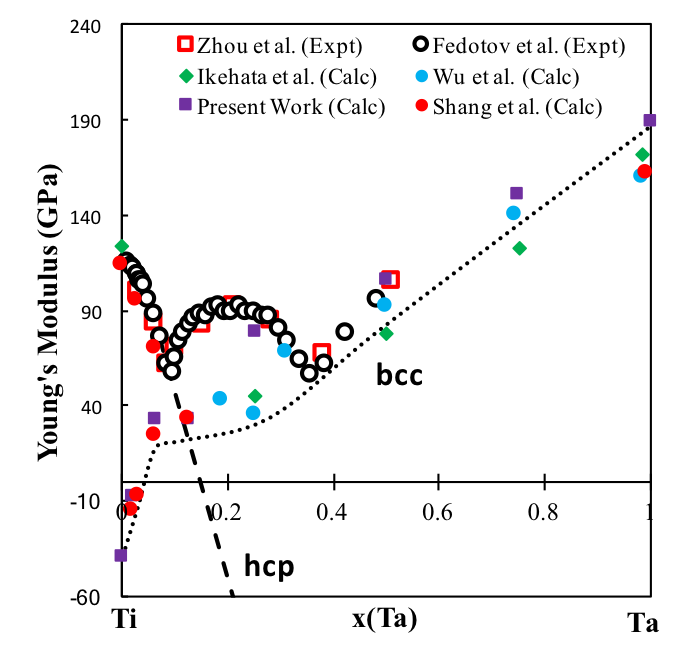
\includegraphics[width=\textwidth]{Chapter-1/Figures/TiTaElastic.png}
	\caption{Comparison of first-principles calculations \cite{Wu2010a,Ikehata2004} and experimental measurements of the Young's modulus of Ti-Ta alloys \cite{Zhou2004a,Zhou2009a,Fedotov1985}. The purple box refers to the composition range when the calculations and experimentally determined $E$ do not match up due to the formation of two metastale phases $\omega$ and $\alpha"$}
	\label{Ch1-figure:titaelastic}
\end{figure}
%%%
\chapter{Methodology}

\section{First-Principles Calculations}

In this dissertation, the ground state energy structures, thermodynamic properties and mechanical properties of Ti and Ti-alloys were calculated using first-principles based on Density Functional Theory. The first-principles refers to the calculations originating from "first-principles", meaning that the inputs were the atomic coordinates and atomic numbers. The first-principles method computes the interactions between atoms in a periodic supercell. This was determined using quantum mechanical electronic theory that is based on the electronic charge density and does not rely on any empirical data. This section provides a description of the DFT methodology.

Schr\"odinger's time-independent non-relativistic equation is a solution to the many-body problem of calculating the interactions of positively charged nuclei and negatively charged electrons. The Schr\"odinger equation is:

%%
\begin{equation}
\label{eq: schrodinger}
\left[ \sum_{i=1}^{N} \left( - \frac{\hbar^2}{2m} \nabla_{i}^2 + V_{ext} (r_{i}) \right) + \sum_{i<j} U (r_{i}, r_{j}) \right] \Psi = E_{s} \Psi
\end{equation}
%%

\noindent where the first bracketed part represents the Hamiltonian ($\hat{H}$), $\Psi$ describes the wave function of electrons, and $E_{s}$ describes the energy of the system. The $\hat{H}$ of the system is described by three parts, the first part represents the kinetic energy with $N$ being the total number of electrons in the system, $\hbar$ being Planck's constant and $m$ the mass of an electron. The second term $V_{ext}$ is the external potential and $U$ is the potential of the electron-electron repulsion.

Eq. \ref{eq: schrodinger} can be solved for $\Psi$ assuming the nuclei-nuclei interactions can be neglected due to the Born-Oppenheimer approximation. The Born-Oppenheimer approximation allows the assumption that the motion of the nuclei on the electronic timescale can be ignored, due to the mass difference, with the nuclei being $\sim$ 10$^3$ to 10$^5$ larger than electrons. However, even with this approximation solving Eq. \ref{eq: schrodinger} is difficult due to the electron-electron Columb interactions making the electronic motion correlated and the fact that the many-body problem results in too many variables because there are 3N degrees of freedom. 

Hohenberg-Kohn formulated two theorems to simplify this problem \cite{Hohenberg1964}. The first theorem states that the external potential is a unique functional of the electron density. The second theorem states that the density that minimizes the total energy is the exact ground state density and thus the ground state is obtained variationally. With these theorems, Kohn-Sham proved that the problem can be solved as if the electrons are not interacting and still obtain the density as if they were, by \cite{Kohn1965}:
 
 \begin{equation}
 \label{eq: kohnsham}
\left[ -\frac{\hbar^2}{2m} \nabla^{2} + V_{ext} (r) + V_{Hartree}(r) + V_{XC} (r) \right] \phi_{1}(r) = \epsilon_{i} \psi_{i}(r)
 \end{equation}
 %%
 
 \noindent where $V_{ext}(r)$ describes the electron-nuclei interaction similar as in Eq. \ref{eq: schrodinger} and is expressed by:

\begin{equation}
\label{eq: vext}
V_{ext} = - e^2 \sum_{a} \frac {Z_{a}}{|r_i - R_a|}
\end{equation}

\noindent where $r_i$ represents the position of electron $i$ and $R_a$ represents the position of nucleus $a$ with a charge valance of $Z_a$. The electron-electron interactions are represented by $V_{Hartree}$:

\begin{equation}
\label{eq: vhartree}
V_{Hartree} (r) = e^{2} \int \frac {\rho(r)}{|r - r_{j}|} d^3r
\end{equation}
%%

\noindent where $r$ and $r_j$ represent the electrons and $\rho (r)$ is described by:

\begin{equation}
\label{eq: rhop}
\rho (r) = \sum_{i}^N | \psi_{i} (r) |^2
\end{equation}
%%

\noindent The final term, $V_{xc}$, is the exchange correlation potential that is described in terms of an exchange-correlation energy. While there is no exact solution to the exchange-correlation (X-C) energy available, there are multiple different approximations. Each approximation is done to account for different things. In the present work, the generalized gradient approximation by Perdew and Wang (PW91) \cite{Perdew1992} and the generalized gradient approximation by Perdew, Burke and Ernzerhoff (PBE) \cite{Perdew1996a} were used. The generalized gradient approach improves the total energies and atomization energies compared to other methods such as the local density approximation \cite{Ceperley1980} but can over-correct for the expansion and softening of bonds. The generalized gradient approximation (GGA) is favored for inhomogeneous densities. Based on previous research by Perdew et al. \cite{Perdew1996a}, GGA's are considered to be adequate approximations for calculating metals. The PW91 X-C functional was designed to satisfy as many exact conditions as possible and thus has some issues. Perdew introduced the PBE X-C functional as an improvement to PW91 to satisfy less exact conditions and only looked at the ones that were energetically significant for metals. The use of PW91 vs PBE was compared for the elastic results of the Ti-Ta system. The results are discussed in detail in chapter 5 and based on the results the PBE X-C functional was chosen in the present thesis work. By implementing the theorems and the Kohn-Sham equation, the energy of the system can thus be calculated.

\subsection{Density Functional Theory at 0 K}

The ground state energy at 0 K without the contribution of zero-point vibrational energy was calculated by using the equation of states (EOS) fitting for the relationship between the energy and volume of the structure. The EOS fitting was achieved through an energy-volume ($E_{0}-V$) curve of 5 or more relaxed volumes and using the four-parameter Birch-Murnaghan (BM4) EOS \cite{Shang2010}:

%%
\begin{equation}
\label{eq: zeroenergy}
E_{0}(V) = a + bV^{\frac{-2}{3}} + cV^{\frac{-4}{3}} + dV^{-2}
\end{equation}
%%

\noindent where $a$, $b$, $c$ and $d$ are fitting parameters. From this equation, the equilibrium properties of a structure can be obtained such as, volume $V_0$, ground state energy $E_{0}$, bulk modulus $B$, and first derivative with respect to pressure $B'$. 

From the ground state energies, the enthalpy of formation at 0 K was calculated by:

%%
\begin{equation}
\label{eq: hform}
H_{Form} = H_{X_{s}Y_{r}} - \left( s H_{X}^{SER} + rH_{Y}^{SER} \right) 
\end{equation}
%%

\noindent where $H_{X_{s}Y_{r}}$ is the enthalpy of a specific structure at a specific composition ($X_{s}Y_{r}$) and $s$ and $r$ are the mole fractions of elements $X$ and $Y$, respectively. $H_{X}^{SER}$ and $H_{Y}^{SER}$ are the enthalpies of the pure elements $X$ and $Y$ in their standard element reference (SER) at standard temperature and pressure. The SER states of the pure elements are hcp Ti, bcc Mo, bcc Nb, bcc Ta, and hcp Zr. The formation energy can be calculated the same way using the energy values instead of enthalpy. The valance configuration for each element was selected based on the Vienna Ab-initio Software Package (VASP) recommendations \cite{Kresse1996}. The p electrons were treated as valance electrons for the Mo and Ta, the d electrons were treated as valance electrons for Sn and the s electrons were treated as valance electrons for Ti, Nb, and Zr \cite{Kresse1996,Kresse1999}.

\subsection{Finite-temperature thermodynamics}

The Helmholtz energy, $F(V,T)$, was calculated, as a function of temperature $T$ and volume $V$ using first-principles based on DFT:
 %%
 \begin{equation}
 \label{eq: helmholtz}
 F(V,T) = E_{0}(V) + F_{vib}(V,T) + F_{T-el}(V,T)
 \end{equation}
 %%
 
\noindent where $E_0$ is the static contribution at 0 K calculated from Eq. \ref{eq: zeroenergy}, $F_{vib}$ is the temperature-dependent vibrational contribution, and $F_{T-el}$ is the thermal electronic contribution. At ambient pressure, the Helmholtz energy of the system is equal to the Gibbs energy, which is used in the CALPHAD modeling. The vibrational contribution was obtained through the phonon quasiharmonic supercell (phonon approach) or the Debye-Gr\"uneisen method (Debye). The phonon approach is a more accurate approach than the Debye model but it is also more computationally expensive. In the present work, both the phonon and Debye models are used in different sections. The vibrational contribution obtained through phonon calculations of at least five different volumes is expressed by \cite{Wang2012}:

%%
\begin{equation}
\label{eq: phonon}
F_{vib}(V,T) = k_{b}T \int_{0}^{\infty} ln \left[ 2sinh \frac{\hbar \varrho}{2k_BT} \right] g(\varrho) d\varrho
\end{equation}
%%

\noindent where $g(\varrho)$ is the phonon density of states as a function of phonon frequency $\varrho$ at volume $V$. $\varrho$ is normally expressed in the literature as $\omega$, however, due to the extensive discussion of the $\omega$ phase in this work the phonon frequency is expressed as $\varrho$ to avoid confusion. In addition, the Debye model is used to estimate the vibrational contribution by \cite{Shang2010}: 

%%
\begin{equation}
\label{eq: debye}
F_{vib}(V,T) = \frac{9}{8} k_{b} \theta_{D}(V) + k_{B}T \left[ 3 ln \left( 1 - e^{\frac{-\theta_{D}}{T}} \right) - D \left( \frac{\theta_D}{T} \right) \right] 
\end{equation}
%%

\noindent where $\theta_{D}$ is the Debye temperature, $T$ is the temperature, and $D \left( \frac{\theta_{D}}{T} \right) $ is the Debye function. $\theta_{D}$ is calculated through: 

%%
\begin{equation}
\label{eq: debyetemp}
\theta_{D} = s \frac{(6\pi^2)^{\frac{1}{3}}\hbar}{k_B} V_{0}^{\frac{1}{6}} \left( \frac{B}{M} \right)^{\frac{1}{2}} \left( \frac{V_0}{V} \right)^{\gamma} 
\end{equation}
%%

\noindent where $s$ is the Debye temperature scaling factor, $\gamma$ is the Gr\"uneisen parameter determined by the pressure derivative of the bulk modulus ($B'$), $B$ is the bulk modulus, $M$ is the atomic mass, and $V_0$ is the equilibrium volume. Here the $V_0$, $B$, and $B'$ are estimated from the EOS fitting using Eq. \ref{eq: zeroenergy}. The Debye temperature scaling factor was determined by Moruzzi et al. \cite{Moruzzi1988} to be 0.617 for nonmagnetic metals. However, this value has been shown to be less accurate for all materials. Liu et al. \cite{Liu2015} extensively studied the Debye scaling factor and how to calculate the scaling factor based on the Poisson's ratio of a material. The methodology by Liu et al. \cite{Liu2015} was used for the present work to calculate the scaling factor: 

%%
\begin{equation}
\label{eq: debyescaling}
s(\nu) = 3^{\frac{5}{6}} \left[ 4\sqrt{2} \left( \frac{1 + \nu}{1 - \nu} \right)^{\frac{3}{2}} + \left( \frac{1 + \nu}{1 - \nu} \right)^{\frac{-1}{3}} \right]
\end{equation}
%%

\noindent where $\nu$ is the Poisson's ratio, which can be calculated from the elastic stiffness coefficients. The calculations are discussed below.

The thermal electronic contribution is based on the electronic density of states and calculated with the Fermi-Dirac statistics \cite{Shang2010,Wang2004}:

%%
\begin{equation}
\label{eq:thermalelectronic}
F_{T-el} = E_{T-el} - T S_{T-el}
\end{equation}
%%

\noindent The $E_{T-el}$ and $S_{T-el}$ represent the energy and entropy of the thermal electron excitations, respectively. The $E_{T-el}$ is expressed by:

%%
\begin{equation}
\label{eq:etel}
E_{T-el} (V,T) = \int n\left(\epsilon, V\right) f \left(\epsilon, T\right) \epsilon d \epsilon - \int^{\epsilon_{f}} n (\epsilon) \epsilon d \epsilon
\end{equation}
%%

\noindent and the entropy $S_{T-el}$ is expressed by:

%%
\begin{equation}
\label{eq:sel}
S_{T-el} (V,T) = -k_{B} \int n(\epsilon, V) \left[ ln f \left(\epsilon,T\right) + \left( 1 - f(\epsilon, T) \right) ln \left( 1 - f \left(\epsilon, T \right) \right) \right] d\epsilon 
\end{equation}
%%

\noindent where $n(\epsilon, V)$ is the electronic density of states (DOS) at energy $\epsilon$,  $f (\epsilon,T)$ is the Fermi-Dirac distribution, $\epsilon_{f}$ is the Fermi energy level and $k_{B}$ is Boltzmann's constant. The Fermi-Dirac distribution $f (\epsilon, T)$ is expressed by:

%%
\begin{equation}
\label{eq:fermidirac}
f (\epsilon,T) = \left[ exp \left( \frac{\epsilon - \mu}{k_{B} T} \right) + 1 \right]^{-1}
\end{equation}
%%

\noindent where $\mu$ is the chemical potential of the electrons. 


\subsection{Elastic stiffness coefficients}

The single crystal elastic stiffness coefficients ($c_{ij}$$'s$) were calculated from the ground state energy structure using a stress-strain method developed by Shang et al. \cite{Shang2007c}. With this method, a set of independent strains $\varepsilon = (\varepsilon_{1}, \varepsilon_{2}, \varepsilon_{3}, \varepsilon_{4}, \varepsilon_{5}, \varepsilon_{6})$ were imposed on the crystal lattice, where $\varepsilon_{1}$, $\varepsilon_{2}$, and $\varepsilon_{3}$ are the normal strains, $\varepsilon_{4}$, $\varepsilon_{5}$, and $\varepsilon_{6}$ are the shear strains, generating a set of stresses $\sigma = (\sigma_{1}, \sigma_{2}, \sigma_{3}, \sigma_{4}, \sigma_{5},\sigma_{6})$. Hooke's law is then used to calculate the elastic stiffness coefficients: 

%%
\begin{equation}
\label{eq: hookes}
\begin{pmatrix}
	c_{11} & c_{12} & c_{13} & 0 & 0 & 0\\
	c_{12} & c_{22} & c_{23} & 0 & 0 & 0\\
	c_{13} & c_{23} & c_{33} & 0 & 0 & 0\\
	0 & 0 & 0 & c_{44} & 0 & 0\\
	0 & 0 & 0 & 0 &  c_{55} & 0\\
	0 & 0 & 0 & 0 & 0 & c_{66} \\    		
\end{pmatrix} =
\begin{pmatrix}
	\varepsilon_{1,1} & & \varepsilon_{1,n}\\
	\varepsilon_{2,1} & & \varepsilon_{2,n}\\
	\varepsilon_{3,1} & ... & \varepsilon_{3,n}\\
	\varepsilon_{4,1} & & \varepsilon_{4,n}\\
	\varepsilon_{5,1} & & \varepsilon_{5,n}\\
	\varepsilon_{6,1} & & \varepsilon_{6,n}\\					
\end{pmatrix}^{-1}
\begin{pmatrix}
	\sigma_{1,1} & & \sigma_{1,n}\\
	\sigma_{2,1} & & \sigma_{2,n}\\
	\sigma_{3,1} & ... & \sigma_{3,n}\\
	\sigma_{4,1} & & \sigma_{4,n}\\
	\sigma_{5,1} & & \sigma_{5,n}\\
	\sigma_{6,1} & & \sigma_{6,n}\\					
\end{pmatrix}
\end{equation}
%%

\noindent where "-1" represents the pseudo-inverse. Due to symmetry, the bcc structure has only three independent elastic stiffness cefficients. However, with a lack of bcc stability for some of the calculations, all of the elastic stiffness coefficients were calculated and the average $\overline{C}_{11}$, $\overline{C}_{12}$ and $\overline{C}_{44}$ values were used:

%%
\begin{equation}
\label{eq: averagec11}
\overline{C}_{11} = \frac{(c_{11} + c_{22} + c_{33})}{3}
\end{equation}
%%

%%
\begin{equation}
\label{eq: averagec12}
\overline{C}_{12} = \frac{(c_{12} + c_{13} + c_{23})}{3}
\end{equation}
%%

%%
\begin{equation}
\label{eq: averagec44}
\overline{C}_{44} = \frac{(c_{44} + c_{55} + c_{66})}{3}
\end{equation}
%%

\noindent This case is for the unstable bcc elastic calculations to mimic the behavior of a cubic structure. The largest variance between the similar elastic stiffness coefficients, when calculating the average, was used to show the deviation from the bcc symmetry in the calculations, shown as error bars. The stable bcc structures show no variance and thus no error bars. To examine the effects of different strain on the elastic properties, three groups of non-zero strain magnitudes, $\pm$0.01, $\pm$0.03, and $\pm$0.07, were tested and the results are discussed in chapter 5. After testing, the $\pm$0.01 was used for all the calculations. The polycrystalline elastic properties including bulk ($B$), shear ($G$), and Young's ($E$) modulus were calculated from the elastic stiffness coefficients, based on the Voigt-Reuss-Hill approach \cite{Simmons1971b}. The Voigt gives the upper elastic bound due to the assumption of constant strain in all grains, the Reuss gives the lower elastic bound due to the assumption of constant stress in all grains, and the Hill approach is the average of Voigt and Reuss and is closer to real values \cite{Zuo1993,Chung1967}. The Hill approach is hence what is listed in the results section. The Voigt and Reuss bounds were also plotted in the figures to give the bounds of the moduli values.

In order to fully investigate the effects of the alloying elements on the Ti-alloys, the mechanical stability of the bcc phase was studied. The mechanical stability is given by Born's criteria for a cubic crystal  \cite{Born1998,Nye1985}:


\begin{equation}
\label{eq: born1}
\overline{C}_{11} -|\overline{C}_{12}| > 0
\end{equation}
\begin{equation}
\label{eq: born2}
\overline{C}_{11} + 2\overline{C}_{12} > 0
\end{equation}
\begin{equation}
\label{eq: born3}
\overline{C}_{44} > 0
\end{equation}

\noindent Based on Born's criteria, when $\overline{C}_{11} - \overline{C}_{12}$ becomes negative then the phase, bcc in this case, loses its mechanical stability and thus $\overline{C}_{11} - \overline{C}_{12}$ is plotted in the results section.

\subsection{Special quasirandom structures (SQS)}

To calculate the energies, enthalpies of formation and elastic properties across the entire binary and ternary composition range, varying compositions of special quasirandom structures (SQS) were used. The SQS are small supercells used to mimic randomly substituted structures in terms of correlation functions. The binary and ternary bcc SQS, used in the present work, were previously generated by Jiang et al.\cite{Jiang2004,Jiang2009}. The relaxation of these SQS structures is complicated because local atomic relaxations can cause the structure to lose the desired lattice symmetry which is far from the original bcc lattice. To preserve symmetry, the calculations were carried out with three different relaxation schemes: 1) the cell volume, cell shape, and ionic positions are simultaneously relaxed, 2) the cell volume and shape are simultaneously relaxed, and 3) only the cell volume is relaxed. The relaxed structure with the lowest energy that preserved the bcc symmetry was used. There are two ways to verify whether the SQS is still bcc or not after the relaxations. The first is to merge different elements into one element, and then, use codes available to check the symmetry or space group (such as VASP \cite{Kresse1999} and phonopy \cite{Togo2008}). The second is to visualize the structure directly using a visualization software and compare the symmetry to the unrelaxed bcc structure. For the present work, the relaxed structures were plotted with a visualization software and compared to the unrelaxed structure. After the relaxation, at least five different volumes were generated and the ions were allowed to relax. This yields the different volumes needed for the EOS fitting described above, which allows a better prediction of the different properties as a function of composition. 

\subsection{First-principles calculation error/difference}

The error/difference between the previous results (experimental or calculation) and present results was calculated using:

%%
\begin{equation}
\label{eq: error}
\sqrt{\frac{\Sigma[(A_{calc}-A_{ref})]^{2}}{\kappa}} = Difference/Error
\end{equation}
%%

\noindent where $A_{calc}$ is from the present calculation and $A_{ref}$ is from the previous experiment or calculation, and $\kappa$ is the total number of data points. 

\section{CALPHAD method}

The CALPHAD method evaluates parameters to represent the Gibbs energy of individual phases as a function of temperature, pressure and composition. Thermochemical and phase boundary data obtained from experiments and first-principles calculations were used in the PARROT module of Thermo-Calc to evaluate the thermodynamic interaction parameters \cite{Andersson2002}. The Gibbs free energy is described by enthalpy $H$, temperature $T$ and entropy $S$ as follows:

%%
\begin{equation}
\label{eq: gibbs}
G = H - T S 
\end{equation}
%%

\noindent The Gibbs energy is then parameterized and expressed by:

%%
\begin{equation}
\label{eq: parameterizaiton}
G - H^{SER} = a + bT + cT ln T + d T^2 + \sum_{2}^{n} e_{n} T^{n}
\end{equation}
%%

\noindent where $H^{SER}$ refers to the elemental enthalpy in the SER state and $a$, $b$, $c$, $d$, $e$ are coefficients. Other thermodynamic properties such as enthalpy, entropy and heat capacity can be derived from this equation. The parameterized equations for the pure elements have been determined and widely adopted from the SGTE to ensure global compatibility between different databases \cite{Dinsdale1991}.

\subsection{Solution phases}

The databases were built upon the pure elements and then the effects of the binary and ternary interactions are modeled. Normally, the effects of alloying are modeled as solution phases or stoichiometric phases. The solution phases with one sublattice are described by: 

%%
\begin{equation}
\label{eq: gibbssolution}
G_m^{\phi} = \sum x_{A} ^{0}G_{A}^{\phi} + R T \sum x_{A} ln x_{A} + ^{XS}G_{m}^{\phi}
\end{equation}
%%

\noindent where $x_{A}$ is the mole fraction of element $A$ and $^{0}G_{A}^{\phi}$ is the molar Gibbs energy of pure element $A$ in the specific phase ($\phi$) being modeled and this is summed for all elements in the alloy system of interest. The second term describes the ideal interaction between elements and is again summed for every element in the alloy system of interest. The last term represents the excess mixing energy, representing the non-ideal interactions between different species $A$ and $B$. The non-ideal interactions are modeled between every set of binary and ternary elements in the system of interest. The excess mixing energy can be expressed by the Redlich-Kister polynomial as \cite{Redlich1948b}: 

%%
\begin{equation}
\label{eq: gibbexsol}
^{XS}G_m^{\phi} = \sum x_{A} x_{B} \sum_{k=0} ^{k}L_{A,B}^{\phi} (x_{A} - x_{B})^k
\end{equation}
%%

\noindent where $L_{A,B}^{\phi}$ represents the interaction parameter for elements $A$ and $B$ in phase $\phi$ described by:

%%
\begin{equation}
\label{eq: binip}
L_{A,B}^{\phi} = ^{k}a + ^{k}bT
\end{equation}
%%

\noindent where $^{k}a$ and $^{k}b$ are evaluated model parameters. Eq. \ref{eq: gibbexsol} can be extended to multi-component systems as:

%%
\begin{multline}
\label{eq: gibbexsolmulti}
^{XS}G_m^{\phi} = \sum x_{A} x_{B} \sum_{k=0} ^{k}L_{A,B}^{\phi} (x_{A} - x_{B})^k + \sum x_{A} x_{B} x_{C} \\ \left[ ^{0}L_{A, B, C}^{\phi} (x_{A} + \delta_{A, B, C} + ^{1}L_{A, B, C}^{\phi} (x_{B} + \delta_{A, B, C} + ^{2}L_{A, B, C}^{\phi} (x_{c} + \delta_{A, B, C} ) \right]
\end{multline}
%%

\noindent where the ternary interaction parameters $L_{A, B, C}^{\phi}$ are described the same as the binary interaction parameters in Eq. \ref{eq: binip} and $\delta_{A, B, C}$ is defined as $\delta_{A, B, C} = ( 1 - x_{A} - x_{B} - x_{C})/3$.

Many alloys go through a disorder to order transition within a phase which requires modeling both the ordered and disordered part. For example, at low temperatures in many of the Ti-containing binary alloys, the randomly substituted bcc phase goes through a second order transition to become the ordered bcc\#2 phase (CsCl-type). In the present work, no modeling is done for the ordered bcc\#2 phase. However, previous modeling of the bcc\#2 phase is incorporated in to the database. The modeling of ordered phases was discussed extensively by Ansara \cite{Ansara1998}.

\subsection{Stoichiometric compounds}

The Gibbs energy of stoichiometric compounds was modeled in per mole unit formula. For the stoichiometric compound, $A_{p}B_{q}$, the Gibbs energy is expressed by \cite{Zacherl2012}: 

%%
\begin{equation}
\label{eq: stoichiometric}
^{0}G_{m}^{A_{p}B_{q}} = a + bT + p * ^{0}G_{A}^{SER} + q * ^{0}G_{B}^{SER}
\end{equation}
%%

\noindent where $a$ and $b$ are the evaluated parameters, $^{0}G_{A}^{SER}$ is the Gibbs energy of pure element $A$ in the SER phase, $^{0}G_{B}^{SER}$ is the Gibbs energy of pure element $B$ in the SER phase, $p$ is the number of atoms per unit formula of element $A$, and $q$ is the number of atoms per unit formula of element $B$.

\subsection{Elastic Properties}

To obtain the elastic properties as a function of composition, the CALPHAD modeling approach was adopted and the Redlich-Kister polynomial was used to describe the elastic stiffness coefficients by \cite{Redlich1948b,Liu2009,Lukas2007,Liu2010}: 

%%
\begin{equation}
\label{eq: elastic}
E(x) = \sum x_{A} E_{A}^{\phi} + \sum x_{A} x_{B}  L_{A,B}^{\phi} + \sum x_{A} x_{B} x_{C}  L_{A, B, C}^{\phi}
\end{equation}
%%

\noindent where similar to Eq. \ref{eq: gibbexsol} and \ref{eq: gibbexsolmulti} the $x_A$, $x_B$, and $x_C$ refer to the mole fraction of element $A$, $B$, and $C$ respectively, $E_{A}$ is the elastic property of element $A$, $L_{A,B}^{\phi}$ and $L_{A,B,C}^{\phi}$ are the binary and ternary interaction parameters, respectively. The binary and ternary interaction parameters were described in terms of Eq. \ref{eq: binip} but with solely an $a$ coefficient. For the binary modeling, the addition of one or two interaction parameters were studied to ensure the best fit. For the ternary systems, only one interaction parameter is needed \cite{Liu2009,Saunders1998,Lukas2007}. The fittings of the binary and ternary interaction parameters were completed using the Mathematica code in appendix C. The binary interaction parameters were fitted using the difference between the linear combination of pure elements and the first-principles results for each Ti-X (X= Mo, Nb, Sn, Ta, Zr) composition. The ternary interaction parameters were fitted using the difference between the interpolation of the pure elements and binary interaction parameters and the first-principles based on DFT results. The present work evaluated interaction parameters for the elastic stiffness coefficients and incorporated them into a database. Pycalphad \cite{Otis2017} was then used to calculate the moduli values as a function of composition based on the Voigt-Reuss-Hill approach.


\section{Experimental}

\subsection{Ti-Nb sample preparation}

To study the effect of the metastable phase formation on Ti-alloys, two sets of Ti-Nb alloy samples were prepared. Each set contained one sample with 0.10, 0.12, 0.18, and 0.20 mole fractions of Nb and 0.90, 0.88, 0.82, 0.80 mole fractions of Ti, respectively. The samples were made using pieces of Ti (99.8 \% Ti Alfa Aesar, Chicago, IL, USA, for set one, and 99.8 \% Sigma Aldrich, St. Louis, MO, USA) and Nb (99.8 \% Alfa Aesar, Chicago, IL, USA, for set one and set two). Two different titanium pieces were used because the Alfa Aesar titanium pieces were out of stock but they both had the same purity and thus should not lead to any issues with the data analysis. The alloyed samples were arc melted (MAM1, Edmund Buhler GmbH, Germany) under argon atmosphere. The alloys were machined into a cylindrical shape (0.7 inches in diameter and 0.7 inches in thickness). The samples were then heat treated using a Lindberg 59544 tube furnace. The tube was made of Al$_{2}$O$_{3}$ and was under vacuum. The samples were annealed at 1273 K for 24 hours. The samples from set 1 were quenched in water to form the $\alpha"$ phase. The samples in set 2 were slow cooled to form the $\omega$ phase.

\subsection{Neutron Scattering}

\subsubsection{ARCS}

The inelastic neutron scattering measurements were carried out using the Wide Angular-Range Chopper Spectrometer (ARCS) at the Spallation Neutron Source (SNS) at Oak Ridge National Laboratory. ARCS is a time-of-flight spectrometer meaning that the incident neutron beam energy is fixed and the ARCS detectors measure the neutrons final position and the time elapse. From this information, the data output on ARCS is momentum and energy. The measurements were taken with the samples loaded in a customized vanadium sample holder. The holder was mounted into the furnace and kept under vacuum throughout all measurements. Two incident neutron energies, $E_{i} = 25 meV$ and $E_{i} = 50 meV$, were used at each temperature (300, 500, 700, 900, 1110 K). Vanadium was chosen for the sample holders because vanadium has a very low coherent scattering for neutrons. The empty vanadium sample holder was measured at the same conditions at each temperature. The measurements of the scattering from the empty sample holder and a linear background from the ARCS instrument were subtracted from the data of the sample. 

\subsubsection{Data Analysis}

From the corrected momentum and energy plots of the samples, the diffraction patterns and phonon density of states were obtained.

Diffraction is an elastic scattering process. The intensities of neutrons, with no change in energy, at each momentum are calculated and modeled as a Gaussian function \cite{Young1998,Toraya1986}. In the present work, each alloy sample contained some combination of the bcc, hcp, $\alpha"$ and $\omega$ phases. In order to obtain the phase fractions, diffraction patterns, from the literature, of Ti and Nb in each of the individual phases were combined and fit to the diffraction pattern of the alloy in question. In order to do the fitting, the distance between scattering planes was taken into account for each phase. By fitting the literature diffraction patterns to the diffraction pattern of the alloys being studied the phase fractions were obtained. 

From the energy vs momentum plots the phonon density of states (DOS) was obtained using an iterative method to remove the elastic and multi-phonon contributions to the phonon DOS and thus plot just the single-phonon DOS \cite{Fultz2009,Squires2012}. First, a trial phonon DOS from the momenta vs energy plots was used to calculate the time dependent self-correlation function ($G(t)$) and the mean square atomic displacement $\left< u^{2} \right>$. The trial single-phonon DOS (S'($\varrho$)) was obtained by modifying the measured signal (S($\varrho$)) by suppressing the elastic peak and constraining S($\varrho$) such that dS($\varrho$)/d$\varrho$=0 when $\varrho$ $\rightarrow$ 0 according to the hydrodynamic limit. $\varrho$ is normally expressed in the literature as $\omega$, however, due to the extensive discussion of the $\omega$ phase in this work the phonon frequency is expressed as $\varrho$ to avoid confusion. Using the trial phonon DOS, $G(t)$ was expressed by \cite{Manley2001,Manley2002}:

%%
\begin{equation}
\label{eq: td_selfcorrelation}
G (t) = \int_{- \infty}^{\infty} d \varrho \frac{Z(\varrho)}{\varrho} n(\varrho) e^{- i \varrho t}
\end{equation}
%%


\noindent where $Z(\varrho)$ is the phonon density of states as a function of phonon frequency $\varrho$ and $n(\varrho)$ is the thermal occupancy factor. From $G(t)$ the dynamic structure factor from the incoherent scattering was calculated by \cite{Manley2001,Manley2002}:

%%
\begin{equation}
\label{eq: S_total_inc}
\overline{S}_{total}^{inc} (\varrho) = \sum_{\theta} \frac{1}{2 \pi \hbar} e^{- Q^{2} (\theta, \varrho) \left<u^{2} \right>} \int_{-\infty}^{\infty} dte^{-i \varrho t} e^{\hbar^{2}Q^{2}(\theta, \varrho) G(t)/2M} \left[ e^{\frac{-t^{2}}{2} \left(\frac{\bigtriangleup E (\varrho)}{2\hbar} \right)^{2}} \right]
\end{equation}
%%

\noindent where $e^{-Q^{2}\left(\theta,\varrho \right) \left< u^{2} \right>}$ is the Debye-Waller factor described with the mean square atomic displacement $\left< u^{2} \right>$ \cite{Squires2012}. The anisotropy in the Debye-Waller factor was neglected because the resulting errors were negligible \cite{Manley2001}.  $M$ is the mass of a neutron, $\hbar$ is Planck's constant and the bracketed area is the Gaussian instrument energy resolution. $Q$ is defined by \cite{Manley2001,Manley2002}:

%%
\begin{equation}
\label{eq: Q}
Q(\theta, \varrho) = \sqrt{\frac{2M}{\hbar^{2}} \left( 2E - \hbar \varrho - 2E \sqrt{1-\frac{\hbar \varrho}{E}}cos(2\theta) \right)}
\end{equation}
%%

\noindent From $G(t)$, the incoherent single-phonon $\overline{S}_{1}^{inc}$ and elastic scattering $\overline{S}_{0}^{inc}$ were determined.  $\overline{S}_{0}^{inc}$ and $\overline{S}_{1}^{inc}$ are the zeroth and first order terms in the Taylor expansion of the $\overline{S}_{total}^{inc}$ when $G(t)=0$ and the multi-phonon incoherent scattering ($S_{m}^{inc}$)contribution can be calculated by \cite{Manley2001,Manley2002}:

\begin{equation}
\label{eq: S_inco}
\overline{S}_{m}^{inc} = \overline{S}_{total}^{inc}-\overline{S}_{0}^{inc}-\overline{S}_{1}^{inc}
\end{equation}
%%

\noindent The calculated $\overline{S}_{m}^{inc}$ is then a good approximation for the multiphonon coherent scattering contribution and the single-phonon DOS was calculated by:

\begin{equation}
\label{eq: onephonon}
Z(\varrho) = S_{1}(\varrho)* \frac{\varrho}{n(\varrho)}
\end{equation}
%%

\noindent The procedure was repeated three times to converge the phonon DOS based on previous recommendations that showed three iterations were enough to converge within statistical errors \cite{Manley2001,Manley2002}.
\chapter{Ti-Mo-Nb-Sn-Ta-Zr Thermodynamic Database}

\section{Introduction}

The design of Ti-alloys for biomedical applications necessitates a completed thermodynamic database that will facilitate the prediction of phase compositions and fractions as a function of composition and temperature. However, there is no completed thermodynamic database for the Ti-Mo-Nb-Sn-Ta-Zr system and thus the present work aims at building a complete database with special focus on the Ti-rich alloys and bcc phase models. With this in mind the pure elements have been extensively studied and are widely adopted from the SGTE database \cite{Dinsdale1991}. The modeling of the binary systems has been widely documented with the exception of the Sn-Ta and Mo-Sn systems, while the ternary systems have been studied experimentally but not been modeled. The Mo-Sn and Sn-Ta subsystems have high melting temperatures and little to no experimental data. In these cases, first-principles calculations based on DFT can be used to aid in modeling and supplement the lack of experimental data. The complete modeling of the Sn-Ta system is discussed in Chapter 4.  

While the alloys in this Ti system have been studied experimentally, yielding phase equilibrium data, only limited calorimetry data is available. With the present work focused on bcc Ti-rich alloys, first-principles calculations based on DFT of the enthalpy of formation of the bcc phase were calculated. The thermodynamic descriptions were built or evaluated using the available experimental phase boundary data and present calculated thermochemical data. In the present chapter, the thermodynamic descriptions of the Ti-Mo-Nb-Sn-Ta-Zr system are described.

\section{Computational details}

First-principles results based on Density Functional Theory (DFT) are used to predict the enthalpy of formation of specific phases. In the present work, the enthalpy of formation of the bcc phase was calculated for the Ti-X and Ti-X-Y (X$\neq$Y= Mo, Nb, Sn, Ta, Zr) systems using the calculated energy of the pure elements in their SER states. For each binary system, 3 special quasirandom structures at different compositions, Ti$_{0.25}$X$_{0.75}$, Ti$_{0.50}$X$_{0.50}$, Ti$_{0.75}$X$_{0.25}$, were calculated (X= Mo, Nb, Sn, Ta, Zr). The SQS were each 16-atom supercells that were previously generated and relaxed according to the methodology in chapter 2 \cite{Jiang2004}. For each binary system other dilute compositions were calculated, i.e. Ti-Mo 4 dilute structures (Mo$_{0.98}$Ti$_{0.02}$ 54-atoms, Mo$_{0.94}$Ti$_{0.06}$ 16-atoms,  Ti$_{0.88}$Mo$_{0.12}$ 8-atoms, Ti$_{0.94}$Mo$_{0.06}$ 16-atoms), Ti-Nb 4 dilute structures (Nb$_{0.98}$Ti$_{0.02}$ 54-atoms, Nb$_{0.94}$Ti$_{0.06}$ 16-atoms, Ti$_{0.88}$Nb$_{0.12}$ 8-atoms, Ti$_{0.98}$Nb$_{0.02}$ 54-atoms), Ti-Sn 1 dilute structure (Ti$_{0.94}$Sn$_{0.06}$ 16-atoms), Ti-Ta 5 dilute structures (Ta$_{0.98}$Ti$_{0.02}$ 54-atoms, Ta$_{0.94}$Ti$_{0.06}$ 16-atoms, Ti$_{0.88}$Ta$_{0.12}$ 8-atoms, Ti$_{0.94}$Ta$_{0.06}$ 16-atoms, Ti$_{0.98}$Ta$_{0.02}$ 54-atoms), and Ti-Zr 2 dilute structures (Zr$_{0.94}$Ti$_{0.06}$ 16-atoms, Ti$_{0.98}$Zr$_{0.02}$ 54-atoms). A different number of dilute structures were done based on the complexity of some of the structures being unstable. For the Ti-X-Y (X $\neq$ Y= Mo, Nb, Sn, Ta, Zr) ternary systems, three SQS calculations were completed at the compositions Ti$_{0.33}$X$_{0.33}$Y$_{0.33}$ (36-atom), Ti$_{0.50}$X$_{0.25}$Y$_{0.25}$ (32-atom), Ti$_{0.74}$X$_{0.13}$Y$_{0.13}$ (64-atom). In order to be able to effectively visualize the DFT-based first-principles results for the Ti-X-Y systems versus the modeling the plots went from a 50-50 binary mixture of the alloying elements to pure Ti. For this graph, DFT-based first-principles results for the binary SQS structure (X$_{8}$Y$_{8}$ 16-atom) at the 50-50 mixture of alloying elements X and Y (XY=Mo, Nb, Ta, Zr) were completed. The binary and ternary SQS were previously generated and also relaxed according to the details outlined in chapter 2 \cite{Jiang2009,Jiang2004}. The DFT calculations are completed using VASP (Vienna ab-initio Simulation Package) \cite{Kresse1996}. The ion-electron interactions were described using the projector augmented wave (PAW) \cite{Kresse1999,Blochl1994} method. Based on the work of comparing X-C functionals (Figure \ref{Ch5-figure:PBEvsPW91}), the exchange-correlation functional of the generalized gradient approach depicted by Perdew, Burke, and Ernzerhof (PBE) was employed \cite{Perdew1996a}. For consistency, a 310 eV energy cutoff was adopted for all calculations, which is roughly 1.3 times higher than the default values suggested by VASP for the elements Ti, Mo, Nb, Sn, Ta, and Zr. The energy convergence criterion of the electronic self-consistency was set as 10$^{-6}$ eV/atom, and the Brillouin zone sampling was done with Bl\"ochl corrections \cite{Blochl1994} using a gamma centered Monkhorst-Pack (MP) scheme \cite{Kresse1996,Monkhorst1976a}. The k-points grid for each calculation are listed in appendix C.

\section{Sn binaries and ternaries}

The thermodynamic description of the Mo-Sn system has never been modeled and there is little to no experimental data available. With this fact, first-principles calculations can be used to fill in the missing data points. However, this is not a hugely important sub-system and the modeling will be part of the future work. The Sn-Ta system is modeled in chapter 4. For the Sn-Zr system, the thermodynamic description was previously modeled. However, these models do not use compatible sublattice modeling with the current database. While the, Nb-Sn and Ti-Sn binary systems have been previously modeled, Sn will only be included in small percentages to the overall Ti-based alloy and until the rest of Sn binaries are modeled, Sn will not be included in the database.

\section{Pure element calculation results}

In order to build the Ti-Mo-Nb-Ta-Zr thermodynamic database, thermodynamic descriptions for the all the binary systems are evaluated first for accuracy and model compatibility (see Chapter 2) and incorporated into the database. For the ternary systems, only thermodynamic descriptions for the Ti-containing ternary systems are developed, including Ti-Mo-Nb, Ti-Mo-Ta, Ti-Mo-Zr, Ti-Nb-Ta, Ti-Nb-Zr, and Ti-Ta-Zr. The thermodynamic description of a non Ti-containing Mo-Nb-Ta ternary system \cite{Xiong2004} is incorporated in the present database. 

Table \ref{Ch3-table:pspureele} shows the energy $E_{0}$, bulk modulus $B$, and the lattice parameters of the pure elements obtained from Eq. \ref{eq: zeroenergy} at 0 K. The values are compared with previous first-principles calculations at 0 K and experimentally obtained values both from the literature. The comparison shows a good agreement. The variances between the present calculations and previous calculations can be attributed to the different input parameters such as a different exchange correlation functional (PBE vs PW91) and higher energy cutoff values. The differences between the present calculations (0 K) and experimental values (300 K) can be partially attributed to the temperature difference. Based on the small variances shown in Table \ref{Ch3-table:pspureele}, the present calculations are deemed accurate. 


\section{Enthalpy of formation of bcc phase from first-principles}

The enthalpies of formation of the bcc phase (bcc-$H_{Form}$) for the binary and ternary systems are presented in Table \ref{Ch3-table:binaryhform} and Table \ref{Ch3-table:ternhform}, respectively. As discussed in the methodology chapter, the bcc-$H_{Form}$ is calculated by Eq. \ref{eq: hform}. Table \ref{Ch3-table:binaryhform} shows the first-principles results for binary bcc-$H_{Form}$: the Ti-Mo system goes from positive to negative to positive indicating the formation of a bcc miscibility gap, and the Ti-Nb, Ti-Ta, and Ti-Zr systems, are positive across the entire composition range. Table \ref{Ch3-table:ternhform} shows the values of the ternary bcc-$H_{Form}$.  The bcc-$H_{Form}$ values, for the Ti-Mo-Nb, Ti-Mo-Ta and Ti-Nb-Ta systems, go from positive at pure Ti to negative at X$_{0.50}$Y$_{0.50}$, while bcc-$H_{Form}$ remains positive for the Ti-Mo-Zr, Ti-Nb-Zr, and Ti-Ta-Zr systems. For each system that the bcc-$H_{Form}$ is calculated, the values are compared with the CALPHAD modeling predictions and in some cases, are compared with experimentally obtained results. For some of the systems, when comparing the first-principles results of the bcc-$H_{Form}$ and the CALPAHD modeling prediction of the bcc-$H_{Form}$, no large discrepancies are seen and thus no new modeling is completed. In other cases, comparing the first-principles results of the bcc-$H_{Form}$ and the CALPAHD modeling prediction of the bcc-$H_{Form}$ showed larger discrepancies and then the first-principles bcc-$H_{Form}$ values are used to introduce new bcc interaction parameters. Each binary and Ti-containing ternary system is discussed in detail in the sections below.

\section{Thermodynamic modeling of the ten binary systems}

\subsection{Mo-Nb, Mo-Ta, Nb-Ta}

Figure \ref{Ch3-figure:binary1} shows the calculated phase diagrams for the Mo-Nb, Mo-Ta, and Nb-Ta systems from thermodynamic descriptions in the literature in comparison with experiments. The Mo-Nb, Mo-Ta and Nb-Ta descriptions are adopted from the modeling completed by Xiong et al. \cite{Xiong2004}. Xiong et al. \cite{Xiong2004} who modeled these three binary systems and the Mo-Nb-Ta ternary system. Binary interaction parameters were introduced for the liquid and bcc solution phases. The thermodynamic description, for the Mo-Nb system, was obtained using experimental data from differential thermal analysis that measured both the liquidus and solidus temperatures \cite{Xiong2004}. Xiong et al. \cite{Xiong2004} decided to only use the experiments (shown in Figure \ref{Ch3-figure:binary1} as X and +) that estimated the pure elements melting temperatures reasonably well when evaluating the binary interaction parameters. Xiong et al. \cite{Xiong2004} discussed, that after evaluating the binary interaction parameters for the Mo-Nb system, the experiments, shown by $\circ$, $\bigtriangleup$, $\square$, agreed well with the predicted phase diagram. Even though, the remaining experimental data points ($\diamond$, *) were quite low as compared to the predicted phase diagram, they were also quite low compared to all the other experiments \cite{Xiong2004} and were considered inaccurate. Thus Xiong et al. \cite{Xiong2004} concluded that the thermodynamic description generated is adequate at predicting the experimental data. 

The thermodynamic description, for the Mo-Ta system, was obtained using two sets of experimental data ($\bigtriangleup$, *, $\diamond$, $\square$) \cite{Xiong2004}. These particular experimental data points were chosen because they accurately measured the melting temperatures of Mo and Ta. The predicted phase diagram accurately reproduced the experimental data with the exception of the experimental data \cite{Xiong2004} denoted as "$\circ$". This set of data was 343.15 K higher than all other experimental data. Xiong et. al. \cite{Xiong2004} thought the dataset was not reliable and was thus ignored. 

For the Nb-Ta system, the thermodynamic description was completed using the experimental liquidus data \cite{Xiong2004} depicted in Figure \ref{Ch3-figure:binary1} by $\circ$, $\bigtriangleup$, and $\square$, because it predicts the melting temperatures of Nb and Ta accurately. The experimentally measured solidus temperatures (*) were not used because the data for both Nb and Ta showed discrepancy. The predicted phase diagram reproduces the experimental data well with the exception of the experimental work depicted by $\diamond$. This dataset was ignored because the values were 343.15 K higher than the other experimental values and thus it was determined by Xiong et al. \cite{Xiong2004} to be unreliable. 

The present work agrees with the conclusion reached by Xiong et al. \cite{Xiong2004} that the phase diagrams reproduce the experimental data accurately. The sublattice models used by Xiong et al. \cite{Xiong2004} are compatible with our working database and the binary descriptions are incorporated without any changes. The interaction parameters for the binary systems incorporated into the database are listed in Table \ref{Ch3-table:ip}. 

\subsection{Mo-Zr, Nb-Zr and Ta-Zr}

Figure \ref{Ch3-figure:binary2} shows the predicted phase diagrams for the Mo-Zr, Nb-Zr, and Ta-Zr systems. For the Mo-Zr system, there are several existing thermodynamic descriptions and experimental results available. In the present work, the evaluation by Perez et al. \cite{Perez2003} is chosen to be incorporated due to the fact that their model was also incorporated into the Ti-Mo-Zr ternary modeling found in the literature. The experimental data plotted in Figure \ref{Ch3-figure:binary2} includes the single-phase regions, two-phase regions, phase boundaries, and peritectic and eutectiod reactions ($\blacksquare$, *, +, Y, $\diamond$, $\blacklozenge$, $\square$, $\pentagon$, $\CIRCLE$, $\circ$, $\bigtriangleup$, $\hourglasses$ ). Each symbol represents a different set of data from different authors and Perez et al. \cite{Perez2003} went into more details on the available experimental data and discussed what was included in their evaluation. They \cite{Perez2003} introduced interaction parameters for the liquid, bcc, hcp, and Laves\_C15 phases. The thermodynamic description generally reproduces all experimental data very satisfactorily. 

The thermodynamic description, for the Nb-Zr system, was previously evaluated by Guillermet \cite{Guillermet1991}. Figure \ref{Ch3-figure:binary2} plots the predicted phase diagram with the experimental solidus data ($\diamond$, *) as well as the hcp solvus (Y, $\circ$) and bcc miscibility gap ($\bigtriangleup$, $\square$, +) data \cite{Guillermet1991,Kumar1994a,Abriata1982}. The description includes interaction parameters for the liquid, bcc, and hcp solution phases and reproduces the experimental data well. 

For the Ta-Zr system, the thermodynamic description was also evaluated by Guillermet \cite{Guillermet1995}. There are quite a lot of experimental datasets for this binary system, including phase boundary results from at least five different investigations and thermodynamic results from three different studies \cite{Guillermet1995}. Figure \ref{Ch3-figure:binary2} plots the single-phase ($\CIRCLE$, $\blacksquare$), two-phase ($\circ$, $\square$), and phase boundary (*,+) experimental data in comparison with the CALPHAD results. Interaction parameters were introduced for the bcc, hcp, and liquid phases. The predicted phase diagram reproduces the data fairly well. 

The thermodynamic descriptions of the three binary systems Mo-Zr, Nb-Zr, and Ta-Zr are determined to be accurate and the sublattice modeling used is compatible with our working database. Thus, the thermodynamic descriptions are incorporated into the database. The interaction parameters for the binary systems incorporated into the database are listed in Table \ref{Ch3-table:ip}. 

\subsection{Ti-Mo}

The thermodynamic description in the COST 507 database, modeled by Saunders, \cite{Ansara1998} is looked at for the Ti-Mo system. This model is chosen because it is the model incorporated into the Ti-Mo-Zr thermodynamic modeling \cite{Kar2008}. Interaction parameters were evaluated for the liquid, fcc, hcp, bcc (ordered bcc\#1 and disordered bcc\#2), AlM\_D019, AlM-D022, and the AlTi-L10 phases. Figure \ref{Ch3-figure:TiMo}a compares the predicted phase diagram \cite{Ansara1998} with the available experimental phase boundary data \cite{Murray1981}. The phase boundary data is reproduced very well. Figure \ref{Ch3-figure:TiMo}b plots the predicted enthalpy of formation of the bcc phase (solid line) versus the results from the present DFT-based first-principles calculations (circles) and are compared to the enthalpies of formation of the bcc phase obtained experimentally (red squares) \cite{Uesugi2013}. The experimental bcc-$H_{Form}$ values and the prediction from the model are at 300 K while the first-principles results are at 0 K. The experimental values of bcc-$H_{Form}$ compare well with the calculations but become more negative closer to the Mo-rich side which can be attributed to the temperature difference. The CALPHAD predicted enthalpy of formation of the bcc phase drastically deviates from the first-principles calculation results between 20 and 80 at.\% Mo. This discrepancy is mostly due to the disagreement on the existence of a bcc miscibility gap. Previous experimental research, including the values plotted here, have shown an equilibrium bcc miscibility gap which would fit what is seen in the first-principles calculations \cite{Uesugi2013,Predel1997,Hoffman1967}. While there is an interaction parameter for the bcc order and disorder, Saunders \cite{Ansara1998} did not model the bcc miscibility gap. While there are previous thermodynamic descriptions that model the bcc miscibility gap, Kar et al. \cite{Kar2008} showed that the experimental data from higher-component systems fits better with the description without the miscibility gap. Based on this and the fact that the sublattice modeling is compatible with the working database, the thermodynamic description by Saunders \cite{Ansara1998} is adopted without changes. The interaction parameters for the binary system incorporated into the database are listed in Table \ref{Ch3-table:ip}.


\subsection{Ti-Nb}

For the Ti-Nb system, its thermodynamic description is taken from Zhang et al. \cite{Zhang2001}. Originally the thermodynamic description by Kumar et al. \cite{Kumar1994,Kumar1994a} was evaluated because it was used in the modeling of the Ti-Nb-Zr system. However, new experimental phase boundary data on the Nb rich side ($\bigtriangleup$) showed the need to switch to the thermodynamic description of Zhang et al. \cite{Zhang2001} who introduced interaction parameters for the liquid, bcc, hcp and omega phases. Figure \ref{Ch3-figure:TiNb}a plots the predicted phase diagram from Zhang et al. \cite{Zhang2001} against solidus data ($\square$), hcp and bcc solvus data ($\circ$) \cite{Kumar1994,Kumar1994a} and the new Nb-rich bcc solvus data ($\bigtriangleup$) \cite{Zhang2001}. Figure \ref{Ch3-figure:TiNb}b plots the predicted enthalpy of formation (solid line) versus the present first-principles calculations (circles) and are compared to the enthalpies of formation of the bcc phase obtained experimentally (red squares) \cite{Uesugi2013}. The experimental bcc-$H_{Form}$ values and the prediction from the model are at 300 K while the first-principles results are at 0 K. The experimental bcc-$H_{Form}$ values compare well with the calculations and any variance can be mostly attributed to the temperature difference. There is an average variance of 0.17 kJ/mol-atom between the DFT results and CALPHAD predictions of the bcc-$H_{Form}$ which is also attributed to the temperature difference. However, even with the variance, the CALPHAD prediction compares well with the DFT results and the phase diagram reproduces the experimental data very well. The sublattice models are compatible and the thermodynamic description from Zhang et al. \cite{Zhang2001} is incorporated into the present database with no alterations. The interaction parameters for the binary system incorporated into the database are listed in Table \ref{Ch3-table:ip}.

\subsection{Ti-Ta}

The thermodynamic description for the Ti-Ta system is taken from the COST 507 database \cite{Ansara1998}. The predicted phase diagram is plotted in Figure \ref{Ch3-figure:TiTa}a and compared with the experimental liquidus and solidus data ($\diamond$ and Y) as well as the bcc and hcp solvus data ($\bigtriangleup$, $\square$, and $\circ$). The evaluation includes interaction parameters for the fcc, hcp, liquid, AlM-D019, AlM-D022, AlTi-L10, and the bcc (ordered bcc\#1, disordered bcc\#2) phases \cite{Murray1987}. The thermodynamic description reproduces the experimental data well. The enthalpy of formation of the bcc phase predicted by the CALPHAD modeling (solid line) is plotted with the first-principles results (circles) in Figure \ref{Ch3-figure:TiTa}b. The CALPHAD prediction of the bcc-$H_{Form}$ reproduces the results from first-principles reasonably well on the Ti-rich and Ta-rich sides. The first-principles results vary on an average by 0.17 kJ/mol-atom. However, the CALPHAD prediction is at 300 K and the first-principles are at 0 K which may be mostly responsible for the variance. Based on these discussions, the thermodynamic description is deemed reliable and since the sublattice modeling is compatible, the thermodynamic description is incorporated into the database without alteration. The interaction parameters for the binary system incorporated into the database are listed in Table \ref{Ch3-table:ip}.

\subsection{Ti-Zr}

The thermodynamic description of the Ti-Zr system evaluated by Kumar et al. \cite{Kumar1994a} is used in the present work. The model by Kumar et al. \cite{Kumar1994a} is chosen because it was used in the ternary modeling of the Ti-Mo-Zr and Ti-Nb-Zr systems. The evaluation introduces interaction parameters for the liquid, bcc, and hcp solution phases. Figure \ref{Ch3-figure:TiZr}a compares the predicted phase diagram with phase boundary data for the bcc to hcp ($\circ$) phase transformation and solidus ($\bigtriangleup$). The thermodynamic description accurately reproduces the phase boundary data. When doing the evaluation, heat of transformation data was also used and was discussed by Kumar et al. \cite{Kumar1994a}. Figure \ref{Ch3-figure:TiZr}b plots the present DFT-based first-principles results (circles) against the CALPHAD prediction (solid line) for the bcc-$H_{Form}$. The first-principles results and CALPHAD modeling vary on average by 1.2 kJ/mol-atom. The variance is larger than the other binary alloys due to the instability of the bcc phase at both 0 K and 300 K for the Ti-Zr alloy but the calculations and CALPHAD prediction follow the same trend. Based on the agreement with the experimental data and the compatible sublattice models, no alterations were made to the thermodynamic description which was incorporated into the database. The interaction parameters for the binary system incorporated into the database are listed in Table \ref{Ch3-table:ip}. 

\section{Thermodynamic modeling of six Ti-containing ternary systems}

In this section, the enthalpy of formation of the bcc phase is plotted from a 50-50 mixture of the alloying elements X$_{0.5}$Y$_{0.5}$ to Ti. When doing the evaluations, the enthalpy of formation of the bcc phase was plotted for all compositions. The plot shown here is just the easiest way to show the comparison between the modeling prediction and the DFT-based first-principles results.

\subsection{Ti-Mo-Nb}

There has never been a thermodynamic description for the Ti-Mo-Nb system in literature. Two experimental investigations were performed on the Ti-Mo-Nb system at 873 K and 1373 K \cite{English1961,Prokoshkin1967}. While both investigations agree that the isothermal section at 1373 K is solely the bcc phase, the investigations differed on the phase boundary at 873 K. It is suspected that at such a low temperature the samples were hard to reach equilibrium, which may have led to the discrepancy. Based on this, the binary interpolation of the isothermal sections at 1373 K and 873 K are plotted. The predicted phase diagram at 1373 K agreed with the experimentally determined phase diagram to be solely the bcc phase. The phase diagram at 873 K is plotted in Figure \ref{Ch3-figure:TiMoNb}a. The discrepancy, at 873 K, is the existence of the bcc miscibility gaps as well as what compositions the phase boundary lines lie at. The enthalpy of formation of the bcc phase is predicted using an interpolation of the binary interaction parameters (solid line) and plotted with the first-principles results, in Figure \ref{Ch3-figure:TiMoNb}b, starting from a 50-50 mixture of the alloying elements (Mo$_{0.50}$Nb$_{0.50}$) to 100 at.\% Ti. While the first-principles calculations are at 0 K and the binary interpolation is at 300 K, the DFT-based first-principles calculation results agree with the CALPHAD prediction. The prediction varies by less than 1.5 kJ/mol-atom for all the calculations except at Mo$_{0.50}$Nb$_{0.50}$ where the calculation varies substantially from the prediction. In order to improve this, the Mo-Nb binary system would have to be adjusted. In the present work, no thermochemical data was used to ensure the accuracy of the non Ti-containing binary systems but the previous binary models were able to reproduce the phase boundary data as discussed above. Based on the discrepancy between the experimental data and the fact that the first-principles thermochemical results are reproduced well by the binary interpolation, no ternary interaction parameters are evaluated. 


\subsection{Ti-Mo-Ta}

The thermodynamic description of the Ti-Mo-Ta system has not been previously modeled. The binary interpolation of the Ti-Mo-Ta system is plotted in Figure \ref{Ch3-figure:TiMoTa1}a at 873 K at which the Ti-Mo-Ta system has the bcc and hcp solution phases with the tie-triangle showing a three-phase region in the Ti-rich corner, but did not show a bcc miscibility gap or tie-triangle \cite{Nikitin1971}. Figure \ref{Ch3-figure:TiMoTa1}b shows the present DFT-based first-principles results (circles) of the bcc-$H_{Form}$ compared with the binary interpolation from the CALPHAD prediction (solid black line). The first-principles results line up fairly well with the CALPHAD prediction. However, due to the discrepancy of the experimental data, ternary interaction parameters are investigated for the hcp and bcc phases using the first-principles results and experimental phase boundary data. The evaluated interaction parameters are listed in Table \ref{Ch3-table:ip}. After assessing the ternary interaction parameters, the isothermal section at 873 K is again plotted and compared with experimental data in Figure \ref{Ch3-figure:TiMoTa2}a and zoomed in for Figure \ref{Ch3-figure:TiMoTa2}b. The enthalpy of formation of the newly assessed bcc phase is plotted as a red dashed line in Figure \ref{Ch3-figure:TiMoTa1}b. The assessment reproduces the first-principles results very well. With the introduction of the interaction parameters, the isothermal section agrees well with the experimental data \cite{Nikitin1971}. The hcp phase boundary data from Nikitin \cite{Nikitin1971} were plotted as $\circ$ and two phase experimental data as $\LEFTcircle$. The two phase experimental data is reproduced by the present model. The hcp phase boundary data are not well reproduced. However, reliable solid phase boundary data are difficult to obtain at such a low temperature and if the evaluation is altered to fit the data; it then over fits and stabilizes non-equilibrium phases. 

\subsection{Ti-Mo-Zr}

The thermodynamic description of the Ti-Mo-Zr system was previously modeled by Kar et al. \cite{Kar2008}. The same binary phases used in the modeling by Kar et al. are included in the present database. The phases in this ternary system are liquid, bcc, hcp, and Laves\_C15 (Mo$_{2}$Zr). After interpolating the ternary system from the binary models and comparing to two sets of available experimental data, Kar et al. \cite{Kar2008} introduced interaction parameters for the Laves\_C15 (Mo$_{2}$Zr) phase. After interpolating the ternary system from the binary models and comparing to two sets of available experimental data, Kar et al. \cite{Kar2008} introduced interaction parameters for the Laves\_C15 phase. As discussed by Kar et al. \cite{Kar2008}, there is phase boundary data at 1273 K, from two investigations \cite{Kar2008}. The phase boundary datasets deviate on how far the two-phase region extends toward the Ti-rich corner and whether there is a bcc miscibility gap. Due to the discrepancy, Kar et al. \cite{Kar2008} decided not to introduce any bcc, liquid, or hcp interaction parameters. The prediction of the phase diagram at 1273 K by Kar et al. \cite{Kar2008} is plotted in \ref{Ch3-figure:TiMoZr}a and compared with one set of phase boundary data \cite{Kar2008}. The phase boundary data fits well on the Zr-Mo binary side but extends further in the Ti-rich corner. This is where the discrepancy lies, the other set of phase boundary data, not shown here, shows a shallower two-phase region that the current CALPHAD prediction. The predicted enthalpy of formation of the bcc phase is compared with the present first-principles results in Figure \ref{Ch3-figure:TiMoZr}b. The first-principles results vary by 1.5 kJ/mol-atom from the CALPHAD prediction but the largest variance is seen at Mo$_{0.50}$Zr$_{0.50}$ which would only be improved by adjusting the binary Mo-Zr interaction parameters. Based on the available experimental data \cite{Kar2008}, the present first-principles calculations, and the conclusions from Kar et al. \cite{Kar2008}, the present study decides to include the ternary Laves\_C15 interaction parameters without introducing the ternary interaction parameters for the liquid, bcc, and hcp phases. The ternary Laves\_C15 (Mo$_{2}$Zr) interaction parameters are listed in Table \ref{Ch3-table:ip}.

\subsection{Ti-Nb-Ta}

A thermodynamic description of the Ti-Nb-Ta system had not previously been evaluated in the literature but different isothermal sections had been estimated by Na et al. \cite{Na2001} using phase boundary data obtained through x-ray diffraction. Na et al. \cite{Na2001} looked at samples at 823 K and 673 K. The authors \cite{Na2001} pointed out that it is likely that the alloys at 673 K never reached equilibrium conditions. The experimental results \cite{Na2001} were plotted on the ternary isothermal sections predicted purely based on binary interpolation in Figure \ref{Ch3-figure:TiNbTa1}a and Figure \ref{Ch3-figure:TiNbTa1}b. The bcc phase boundary data do not match with the binary interpolation. Figure \ref{Ch3-figure:TiNbTa2} plots the enthalpy of formation of the bcc phase predicted by the binary interpolation (solid line) and the first-principles results (circles). The first-principles results deviate significantly from the binary interpolation. Due to the variance, ternary interaction parameters for the bcc and hcp phases are investigated. The evaluation was done using the 823 K experimental data and the present first-principles calculations with 673 K data being neglected due to concerns of true equilibrium at such a low temperature. The evaluated ternary interaction parameters are listed in Table \ref{Ch3-table:ip}. After evaluation, the ternary isothermal sections are plotted with the phase boundary data in Figure \ref{Ch3-figure:TiNbTa3}a and Figure \ref{Ch3-figure:TiNbTa3}b. The isothermal sections at both 673 and 823 K reproduce the experimental data \cite{Na2001} well. The assessed prediction (red dashed line in Figure \ref{Ch3-figure:TiNbTa2}) of the enthalpy of formation of the bcc phase also matches better with the first-principles results.

\subsection{Ti-Nb-Zr}

The thermodynamic description, of the Ti-Nb-Zr system was previously evaluated by several studies \cite{Kumar1994a,Tokunaga2007}. In the present work, the binary interpolation of the ternary isothermal section at multiple temperatures are compared with the experimental data \cite{Kumar1994a,Tokunaga2007}. Figure \ref{Ch3-figure:TiNbZr}a plots the isothermal section at 843 K in comparison with the two-phase equilibria data and the tie-triangle phase boundary data \cite{Tokunaga2007}. The binary interpolation reproduced the experimental results well. The enthalpy of formation of the bcc phase is plotted in Figure \ref{Ch3-figure:TiNbZr}b. The CALPHAD prediction (solid line) of the bcc-$H_{Form}$ varies on an average by 1.34 kJ/mol-atom from the first-principles results (circles). While there is some variance, it may be attributed to the temperature difference and overall the variance isn't large. Therefore, a decision was made to not introduce ternary interaction parameters, which is in agreement with past authors \cite{Kumar1994a,Tokunaga2007}.  

\subsection{Ti-Ta-Zr}

For the Ti-Ta-Zr system, Lin et al. \cite{Lin1996} calculated the isothermal sections using binary interpolations without introducing any interaction parameters. The isothermal sections at 1273 and 1773 K are plotted in Figure \ref{Ch3-figure:TiTaZr1}a and Figure \ref{Ch3-figure:TiTaZr1}b, respectively. Experimental phase boundary data along the bcc miscibility gap at 1273 K and single phase $\bullet$ and two phase region $\LEFTcircle$ data using x-ray diffraction at 1773 K are plotted to compare with the binary interpolations \cite{Lin1996,Hoch1964}. The phase boundary data is reproduced well. Figure \ref{Ch3-figure:TiTaZr2} plots the binary interpolation prediction (solid line) of the bcc-$H_{Form}$ compared to the present first-principles results (circles). On average the first-principles varies by 3.69 kJ/mol-atom attributed partially to the temperature difference. While the variance is larger for the enthalpy of formation, the experimental data points \cite{Lin1996} are reproduced and thus no ternary interaction parameters are evaluated

It is worth mentioning that all the interaction parameters for the Ti-Mo-Nb-Ta-Zr system are listed in Table \ref{Ch3-table:ip} and combined into a single thermodynamic database (TDB) file in appendix A.

\section{Conclusion}

The present study builds a compatible and complete thermodynamic database for the Ti-Mo-Nb-Ta-Zr system using descriptions of five pure elements (Ti, Mo, Nb, Ta, Zr), ten binary systems (Ti-Mo, Ti-Nb, Ti-Ta, Ti-Zr, Mo-Nb, Mo-Ta, Mo-Zr, Nb-Ta, Nb-Zr, Ta-Zr), and six Ti-containing ternary systems (Ti-Mo-Nb, Ti-Mo-Ta, Ti-Mo-Zr, Ti-Nb-Ta, Ti-Nb-Zr, Ti-Ta-Zr). Sn was excluded from the database due to the lack of modeling for the Sn binary systems. The Sn-Ta and Mo-Sn systems lacked a thermodynamic description and the thermodynamic modeling of the Sn-Zr system is incompatible with the current database. The present work began modeling the Sn binaries with the Sn-Ta system discussed chapter 4. Until the binaries are properly modeled, Sn was not included in the database which shouldn't affect the use of the database for biomedical applications since Sn will only be added to biomedical alloys in small percentages. The thermodynamic descriptions of the pure elements were adopted from the SGTE database \cite{Dinsdale1991}. All of the binary systems had previous thermodynamic descriptions available in literature. Previous models for all binary systems were evaluated for accuracy and incorporated into the present database. The binary interpolations of the Ti-containing ternary systems were plotted and compared with the available experimental data as well as the enthalpy of formation of the bcc phase calculated from first-principles based on DFT. The Ti-Sn-X systems (X = Mo, Nb, Ta, Zr) will be modeled in the future work once the Sn binaries are modeled. The binary interpolations of both the Ti-Nb-Zr and Ti-Ta-Zr systems had previously been plotted but no interaction parameters had been introduced. The Ti-Mo-Zr system had previously been modeled and the present work agreed with the evaluation. The Ti-Mo-Nb, Ti-Mo-Ta and Ti-Nb-Ta systems had never previously been modeled. The present work evaluated interaction parameters for the Ti-Mo-Ta and Ti-Nb-Ta systems but didn't introduce any interaction parameters for the Ti-Mo-Nb system. The thermodynamic descriptions were all incorporated into a complete database that can reliably predicts the phase stability of the Ti-Mo-Nb-Ta-Zr systems.


\newpage
\begin{table}[H]
	\caption{Equilibrium properties energy $E_{0}$, bulk modulus $B$ and the lattice parameters from the first-principles calculations for each pure elements in their SER state. The presently calculated results are also compared with available experimental data and previously calculated results.}
	\centering
	\begin{tabular}{ c c c c c c }
		\hline
		Phase & $E_{0}$ (eV/atom) & $a (\AA)$ & $c (\AA)$ & $B$ (GPa) & Reference \\
		\hline
		hcp-Ti & -7.80 & 2.92 & 4.6 & 113 & This work\\
		          & -7.89 & 2.93 & 4.64 & 113 & Calc 0 K \cite{Schmitz-Pranghe1968_792,MaterialsProject}\\
                 & & 2.96 & 4.7 & 110 & Expt 300 K \cite{Lame2011,Dobromyslov1987}\\
        bcc-Mo & -10.84 & 2.74 & - & 262 & This work\\
                  & -10.86 & 2.74 & - & 262 & Calc 0 K \cite{Chen_Y2009_794,MaterialsProject}\\
                 & & 2.72 & - & 261 & Expt 300 K \cite{Dickinson1967a,Tsai1992}\\
        bcc-Nb & -10.22 & 2.86 & - & 171 & This work\\
                   & -10.12 & 2.88 & - & 174 & Calc 0 K \cite{Neuburger1936_127,MaterialsProject}\\
                 & & 2.86 & - & 172 & Expt 300 K \cite{Bolef1961,Steinbinder1988} \\
        bcc-Ta & -11.85 & 2.87 & - & 196 & This work\\
                 & -11.85 & 2.87 & - & 194 & Calc 0 K \cite{Neuburger1936_262,MaterialsProject}\\
                 & & 2.86 & - & 196 & Expt 300 K \cite{Bolef1961,Vavilova1988}\\                     
        hcp-Zr & -8.51 & 3.04 & 4.98 & 94 & This work\\
                 & -8.55 & 3.23 & 5.17 & 94 & Calc 0 K \cite{Treco1953_964,Bergerhoff1983,Karlsruhe,MaterialsProject}\\
                 & & 3.23 & 5.15 & 97 & Expt 300 K \cite{Peng2014,Prager1994}\\
		\hline
	\end{tabular}
	\label{Ch3-table:pspureele}
\end{table}

\newpage
\begin{table}[H]
	\caption{First-principles results at 0 K for the enthalpy of formation ($H_{Form}$) of the bcc phase for different mole fractions (x) of alloying element X in the Ti-X binary systems (X = Mo, Nb, Ta, Zr).}
	\centering
	\begin{tabular}{ c c c }
		\hline
		Alloy & Type of Calc & $H_{Form}$ (kJ/mol-atom)\\
		\hline
		Ti & Elemental & 7.29\\
		Mo, Nb, Ta & Elemental & 0.00\\
		Zr & Elemental & 8.19\\
		Ti$_{0.94}$Mo$_{0.06}$ & Dilute & 3.08\\
		Ti$_{0.88}$Mo$_{0.12}$ & Dilute & 2.82\\
		Ti$_{0.75}$Mo$_{0.25}$ & SQS & 1.12\\
		Ti$_{0.50}$Mo$_{0.50}$ & SQS & -3.67\\
		Ti$_{0.25}$Mo$_{0.75}$ & SQS & -5.18\\
		Ti$_{0.06}$Mo$_{0.94}$ & Dilute & 1.79\\
		Ti$_{0.02}$Mo$_{0.98}$ & Dilute & 5.82\\
		Ti$_{0.98}$Nb$_{0.02}$ & Dilute & 6.92\\
		Ti$_{0.88}$Nb$_{0.12}$ & Dilute & 5.88\\ 
		Ti$_{0.75}$Nb$_{0.25}$ & SQS & 7.57\\
		Ti$_{0.50}$Nb$_{0.50}$ & SQS & 8.54\\
		Ti$_{0.25}$Nb$_{0.75}$ & SQS & 1.15\\
		Ti$_{0.06}$Nb$_{0.94}$ & Dilute & 0.59\\
		Ti$_{0.02}$Nb$_{0.98}$ & Dilute & 0.20\\
		Ti$_{0.98}$Ta$_{0.02}$ & Dilute & 7.21\\
		Ti$_{0.94}$Ta$_{0.06}$ & Dilute & 7.04\\
		Ti$_{0.88}$Ta$_{0.12}$ & Dilute & 9.28\\
		Ti$_{0.75}$Ta$_{0.25}$ & SQS & 4.89\\
		Ti$_{0.50}$Ta$_{0.50}$ & SQS & 3.94\\
		Ti$_{0.25}$Ta$_{0.75}$ & SQS & 3.10\\
		Ti$_{0.12}$Ta$_{0.88}$ & Dilute & 0.94\\
		Ti$_{0.02}$Ta$_{0.98}$ & Dilute & 0.28\\
		Ti$_{0.98}$Zr$_{0.02}$ & Dilute & 5.49\\
		Ti$_{0.75}$Zr$_{0.25}$ & SQS & 4.59\\
		Ti$_{0.50}$Zr$_{0.50}$ & SQS & 1.94\\
		Ti$_{0.25}$Zr$_{0.75}$ & SQS & 3.50\\
		Ti$_{0.06}$Zr$_{0.94}$ & Dilute & 5.72\\
		\hline
	\end{tabular}
    \label{Ch3-table:binaryhform}
\end{table}
\clearpage
%%%

\newpage
\begin{table}[H]
	\caption{First-principles results at 0 K for the enthalpy of formation ($H_{Form}$) of the bcc phase for different mole fractions (x) of Ti in the Ti-X-Y ternary systems (X $\neq$ Y = Mo, Nb, Ta, Zr).}
	\centering
	\begin{tabular}{ c c c }
		\hline
		Alloy & Type of Calc & $H_{Form}$ (kJ/mol-atom)\\
		\hline
		Mo$_{0.50}$Nb$_{0.50}$ & SQS & -38.69\\
		Ti$_{0.33}$Mo$_{0.33}$Nb$_{0.33}$ & SQS & 5.08\\
		Ti$_{0.50}$Mo$_{0.25}$Nb$_{0.25}$ & SQS & -2.10\\
		Ti$_{0.74}$Mo$_{0.13}$Nb$_{0.13}$ & SQS & 2.18\\
		Mo$_{0.50}$Ta$_{0.50}$ & SQS & -15.64\\
		Ti$_{0.33}$Mo$_{0.33}$Ta$_{0.33}$ & SQS & -5.34\\
		Ti$_{0.50}$Mo$_{0.25}$Ta$_{0.25}$ & SQS & -1.82\\
		Ti$_{0.74}$Mo$_{0.13}$Ta$_{0.13}$ & SQS & 2.77\\
		Mo$_{0.50}$Zr$_{0.50}$ & SQS & 10.31\\
		Ti$_{0.33}$Mo$_{0.33}$Zr$_{0.33}$ & SQS & 8.36\\
		Ti$_{0.50}$Mo$_{0.25}$Zr$_{0.25}$ & SQS & 7.73\\
		Ti$_{0.74}$Mo$_{0.13}$Zr$_{0.13}$ & SQS & 6.82\\
		Nb$_{0.50}$Ta$_{0.50}$ & SQS & -0.41\\
		Ti$_{0.33}$Nb$_{0.33}$Ta$_{0.33}$ & SQS & 1.82\\
		Ti$_{0.50}$Nb$_{0.25}$Ta$_{0.25}$ & SQS & 3.80\\
		Ti$_{0.74}$Nb$_{0.13}$Ta$_{0.13}$ & SQS & 5.59\\
		Nb$_{0.50}$Zr$_{0.50}$ & SQS & 6.21\\
		Ti$_{0.33}$Nb$_{0.33}$Zr$_{0.33}$ & SQS & 9.82\\
		Ti$_{0.50}$Nb$_{0.25}$Zr$_{0.25}$ & SQS & 10.06\\
		Ti$_{0.74}$Nb$_{0.13}$Zr$_{0.13}$ & SQS & 8.75\\
		Ta$_{0.50}$Zr$_{0.50}$ & SQS & 5.75\\
		Ti$_{0.33}$Ta$_{0.33}$Zr$_{0.33}$ & SQS & 2.98\\
		Ti$_{0.50}$Ta$_{0.25}$Zr$_{0.25}$ & SQS & 2.79\\
		Ti$_{0.74}$Ta$_{0.13}$Zr$_{0.13}$ & SQS & 0.79\\
		\hline
	\end{tabular}
	\label{Ch3-table:ternhform}
\end{table}
\clearpage
%%%

\newpage
\LTcapwidth=\textwidth
\begin{longtable}[H]{ c c c }
	\caption{Modelled binary and ternary thermodynamic parameters for the Ti-Mo-Nb-Ta-Zr system. The thermodynamic description of pure elements is not included. The pure element functions, such as GFCCTI, describe the Gibbs energy (G) of the phase (fcc) for the element (Ti) were adopted from the SGTE database \cite{Dinsdale1991} are listed in the Supplementary TDB (thermodynamic database) file (appendix A).} \label{Ch3-table:ip}\\
		\hline
		Phase & Reference & Interaction Parameter\\
		\hline
		\endhead
		\hline
		\endfoot
		Liquid & \cite{Ansara1998} & $0^\textit{L}_{Ti,Mo} = -9000.0+2.00*T$\\
		          & \cite{Zhang2001} & $0^\textit{L}_{Ti,Nb} = 7406.1$\\
		          & \cite{Ansara1998} & $0^\textit{L}_{Ti,Ta} = 1000.0$\\
		          & \cite{Ansara1998} & $0^\textit{L}_{Ti,Ta} = -7000.0$\\
		          & \cite{Kumar1994a} & $0^\textit{L}_{Ti,Zr} = -967.7$\\
		          & \cite{Xiong2004} & $0^\textit{L}_{Mo,Nb} = 15253.7$\\
		          & \cite{Xiong2004} & $1^\textit{L}_{Mo,Nb} = 10594.2$\\
		          & \cite{Xiong2004} & $0^\textit{L}_{Mo,Ta} = 13978.9$\\
		          & \cite{Perez2003} & $0^\textit{L}_{Mo,Zr} = -24055.1+8.146*T$\\
		          & \cite{Perez2003} & $1^\textit{L}_{Mo,Zr} = -5132.17+4.804*T$\\
		          & \cite{Guillermet1991} & $0^\textit{L}_{Nb,Zr} = 10311.0$\\
		          & \cite{Guillermet1991} & $1^\textit{L}_{Nb,Zr} = 6709.0$\\
		          & \cite{Guillermet1995} & $0^\textit{L}_{Ta,Zr} = 13832.1$\\
		          & \cite{Guillermet1995} & $1^\textit{L}_{Ta,Zr} = -7150$\\
          bcc & \cite{Ansara1998} & $0^\textit{L}_{Ti,Mo} = 2000.0$\\
                  & \cite{Ansara1998} & $1^\textit{L}_{Ti,Mo} = -2000.0$\\
                  & \cite{Zhang2001} & $0^\textit{L}_{Ti,Nb} = 13045.3$\\
                  & \cite{Ansara1998} & $0^\textit{L}_{Ti,Ta} = 12000.0$\\
                  & \cite{Ansara1998} & $1^\textit{L}_{Ti,Ta} = -2500.0$\\
                  & \cite{Kumar1994a} & $0^\textit{L}_{Ti,Zr} = -4346.2+5.49*T$\\
                  & \cite{Xiong2004} & $0^\textit{L}_{Mo,Nb} = -68202.6+29.86*T$\\
                  & \cite{Xiong2004} & $1^\textit{L}_{Mo,Nb} = 8201.3$\\
                  & \cite{Xiong2004} & $0^\textit{L}_{Mo,Ta} = -75129.2+30.00*T$\\
                  & \cite{Xiong2004} & $1^\textit{L}_{Mo,Ta} = 6039.2$\\
                  & \cite{Perez2003} & $0^\textit{L}_{Mo,Zr} = 17936.0+3.10*T$\\
                  & \cite{Perez2003} & $1^\textit{L}_{Mo,Zr} = -991.0+4.30*T$\\
                  & \cite{Xiong2004} & $0^\textit{L}_{Nb,Ta} = 1298.0$\\
                  & \cite{Guillermet1991} & $0^\textit{L}_{Nb,Zr} = 15911.0+3.35*T$\\
                  & \cite{Guillermet1991} & $1^\textit{L}_{Nb,Zr} = 3919.0-1.09*T$\\
                  & \cite{Guillermet1995} & $0^\textit{L}_{Ta,Zr} = 29499.6+2.67*T$\\
                  & \cite{Guillermet1995} & $1^\textit{L}_{Ta,Zr} = -4396.2+4.43*T$\\
                  & \cite{Guillermet1995} & $2^\textit{L}_{Ta,Zr} = -6353.3+4.91*T$\\
                  & This work & $0^\textit{L}_{Ti,Mo,Ta} = -154731.2$\\
                  & This work & $0^\textit{L}_{Nb,Ta,Ti} = -136603.3$\\
                  & This work & $1^\textit{L}_{Nb,Ta,Ti} = -136602.7$\\
          hcp & \cite{Ansara1998} & $0^\textit{L}_{Ti,Mo} = 22760.0-6.00*T$\\      
                  & \cite{Zhang2001} & $0^\textit{L}_{Ti,Nb} = 11742.4$\\
                  & \cite{Ansara1998} & $0^\textit{L}_{Ti,Ta} = 8500.0$\\
                  & \cite{Kumar1994a} & $0^\textit{L}_{Ti,Zr} = 5133.0$\\
                  & \cite{Perez2003} & $0^\textit{L}_{Mo,Zr} = 26753.8+4.56*T$\\
                  & \cite{Guillermet1991} & $0^\textit{L}_{Nb,Zr} = 24411.0$\\
                  & \cite{Guillermet1995} & $0^\textit{L}_{Ta,Zr} = 30051.7$\\
           fcc & \cite{Ansara1998} & $0^\textit{L}_{Ti,Mo} = 16500.0$\\
                  & \cite{Ansara1998} & $0^\textit{L}_{Ti,Ta} = 8500.0$\\
    Al3M$\_$D022 & \cite{Ansara1998} & $0^\textit{L}_{Ti:Ti} = 4*GFCCTI$\\
                            & \cite{Ansara1998} & $0^\textit{L}_{Mo:Mo} = 4*GFCCMO$\\
                            & \cite{Ansara1998} & $0^\textit{L}_{Ti:Mo} = GFCCMO+3.0*GFCCTI$\\
                            & \cite{Ansara1998} & $0^\textit{L}_{Mo:Ti} = 3.0*GFCCMO+GFCCTI$\\
                            & \cite{Ansara1998} & $0^\textit{L}_{Ti:Ta} = GFCCTA+3.0*GFCCTI$\\
         AlM$\_$D019 & \cite{Ansara1998} & $0^\textit{L}_{Ti:Ti} = 4.0+4.0*GHSERTI$\\
                              & \cite{Ansara1998} & $0^\textit{L}_{Mo:Mo} = 4.0*GHCPMO$\\
                              & \cite{Ansara1998} & $0^\textit{L}_{Ta:Ta} = 4.0*GHCPTA$\\
                              & \cite{Ansara1998} & $0^\textit{L}_{Ti:Mo} = 17072.0-4.5*T$\\
                              &                             & $+GHCPMO+3.0*GHSERTI$\\
                              & \cite{Ansara1998} & $0^\textit{L}_{Mo:Ti} = 17072.0-4.5*T$\\
                              &                             & $+3.0*GHCPMO+GHSERTI$\\
                              & \cite{Ansara1998} & $0^\textit{L}_{Ti:Ta} = 6376.0+GHCPTA+3.0*GHSERTI$\\
                              & \cite{Ansara1998} & $0^\textit{L}_{Ta:Ti} = 6376.0+3.0*GHCPTA+GHSERTI$\\
                              & \cite{Ansara1998} & $0^\textit{L}_{Ti:Mo} = 51212.0-13.5*T$\\
                              & \cite{Ansara1998} & $0^\textit{L}_{Mo,Ti:Ti} = 51212.0-13.5*T$\\
                              & \cite{Ansara1998} & $0^\textit{L}_{Mo:Mo,Ti} = 5692.0-1.5*T$\\
                              & \cite{Ansara1998} & $0^\textit{L}_{Ti:Ti,Mo} = 5692.0-1.5*T$\\
                              & \cite{Ansara1998} & $0^\textit{L}_{Ta,Ti:Ta} = 19128.0$\\
                              & \cite{Ansara1998} & $0^\textit{L}_{Ta,Ti:Ti} = 19128.0$\\
                              & \cite{Ansara1998} & $0^\textit{L}_{Ta:Ta,Ti} = 2128.0$\\
                              & \cite{Ansara1998} & $0^\textit{L}_{TI:Ta,Ti} = 2128.0$\\
                       AlTi & \cite{Ansara1998} & $0^\textit{L}_{Ti:Ti} = 2.0*GFCCTI$\\
                              & \cite{Ansara1998} & $0^\textit{L}_{Mo:Mo} = 2.0*GFCCMO$\\
                              & \cite{Ansara1998} & $0^\textit{L}_{Ta:Ta} = 2.0*GFCCTA$\\
                              & \cite{Ansara1998} & $0^\textit{L}_{Ti:Mo} = 8250.0+GFCCMO+GFCCTI$\\
                              & \cite{Ansara1998} & $0^\textit{L}_{Mo:Ti} = 8250.0+GFCCMO+GFCCTI$\\
                              & \cite{Ansara1998} & $0^\textit{L}_{Ti:Ta} = 4250.0+GFCCTA+GFCCTI$\\
                              & \cite{Ansara1998} & $0^\textit{L}_{Ta:Ti} = 4250.0+GFCCTA+GFCCTI$\\
                              & \cite{Ansara1998} & $0^\textit{L}_{Mo,Ti:Mo} = 8250.0$\\
                              & \cite{Ansara1998} & $0^\textit{L}_{Mo,Ti:Ti} = 8250.0$\\
                        & \cite{Ansara1998} & $0^\textit{L}_{Mo:Mo,Ti} = 8250.0$\\
                        & \cite{Ansara1998} & $0^\textit{L}_{Ti:Mo,Ti} = 8250.0$\\
                        & \cite{Ansara1998} & $0^\textit{L}_{Ta,Ti:Ta} = 4250.0$\\
                        & \cite{Ansara1998} & $0^\textit{L}_{Ta,Ti:Ti} = 4250.0$\\
                        & \cite{Ansara1998} & $0^\textit{L}_{Ta:Ta,Ti} = 4250.0$\\
                        & \cite{Ansara1998} & $0^\textit{L}_{Ti:Ta,Ti} = 4250.0$\\
      bcc\#2 & \cite{Ansara1998} & $0^\textit{L}_{Ti:Mo} = 10000.0$\\
  disordered phase & \cite{Ansara1998} & $0^\textit{L}_{Mo:Ti} = 10000.0$\\
                              & \cite{Ansara1998} & $0^\textit{L}_{Ti:Ta} = 5000.0$\\
                              & \cite{Ansara1998} & $0^\textit{L}_{Ta:Ti} = 5000.0$\\
       Laves$\_$C15 & \cite{Kar2008} & $0^\textit{L}_{Ti:Ti} = 15000.0+3.0*GHSERTI$\\
                               & \cite{Perez2003} & $0^\textit{L}_{Mo:Mo} = 15000.0+3.0*GHSERMO$\\
                               & \cite{Perez2003}  & $0^\textit{L}_{Zr:Zr} = 15000.0+3.0*GHSERZR$\\
                               & \cite{Kar2008} & $0^\textit{L}_{Ti:Mo} = 15000.0+GHSERMO$\\
                               &                        & $+2.0*GHSERTI$\\
                               & \cite{Kar2008} & $0^\textit{L}_{Mo:Ti} = 15000.0$\\
                               &                        & $+2.0*GHSERMO+GHSERTI$\\
                               & \cite{Kar2008} & $0^\textit{L}_{Ti:Zr} = 9000.0$\\
                               &                        & $+GHSERZR+2.0*GHSERTI$\\
                               & \cite{Kar2008} & $0^\textit{L}_{Zr:Ti} = 15000.0+2.0*GHSERZR+GHSERTI$\\
                               & \cite{Perez2003}  & $0^\textit{L}_{Mo:Zr} = -21734.8+0.14*T$\\
                               &                             & $+GHSERZR+2.0*GHSERMO$\\
                               & \cite{Perez2003}  & $0^\textit{L}_{Zr:Mo} = 21734.8-0.14*T$\\
                               &                             & $+2.0*GHSERZR+GHSERMO$\\
                               & \cite{Perez2003} & $0^\textit{L}_{Mo:Mo,Zr} = 60000.0$\\
                               & \cite{Perez2003} & $0^\textit{L}_{Zr:Mo,Zr} = 60000.0$\\
                               & \cite{Perez2003}  & $0^\textit{L}_{Mo,Zr:Mo} = 100000.0$\\
                               & \cite{Perez2003}  & $0^\textit{L}_{Mo,Zr:Zr} = 100000.0$\\
                               & \cite{Kar2008} & $0^\textit{L}_{Ti:Mo,Zr} = 60000.0$\\
                               & \cite{Kar2008} & $0^\textit{L}_{Mo,Zr:Ti} = 100000.0$\\
                  omega & \cite{Zhang2001} & $0^\textit{L}_{Ti} = 1886.7-0.15*T+GHSERTI$\\
                               & \cite{Zhang2001} &$0^\textit{L}_{Nb} = 15000.0+2.4*T+GHSERNB$\\
                               & \cite{Dinsdale1991} & $0^\textit{L}_{Zr} = -8878.082+144.432234*T$\\
                               &                               & $-26.8556*T*LN(T)-.002799446*T^{2}$\\                      
                               &      & $+38376*T^{-1}    298.15 < T < 2128$\\
                               &      & $-29500.524+265.290858*T$\\
                               &      & $-42.144*T*LN(T)+7.17445E+31*T^{-9}$\\          
                               &      &  $2128 < T< 6000$\\
                               & \cite{Zhang2001} & $0^\textit{L}_{Ti,Nb} = -3775.9$\\
\end{longtable}
%%%



\newpage
%%%
\begin{figure}[H]
	\centering
	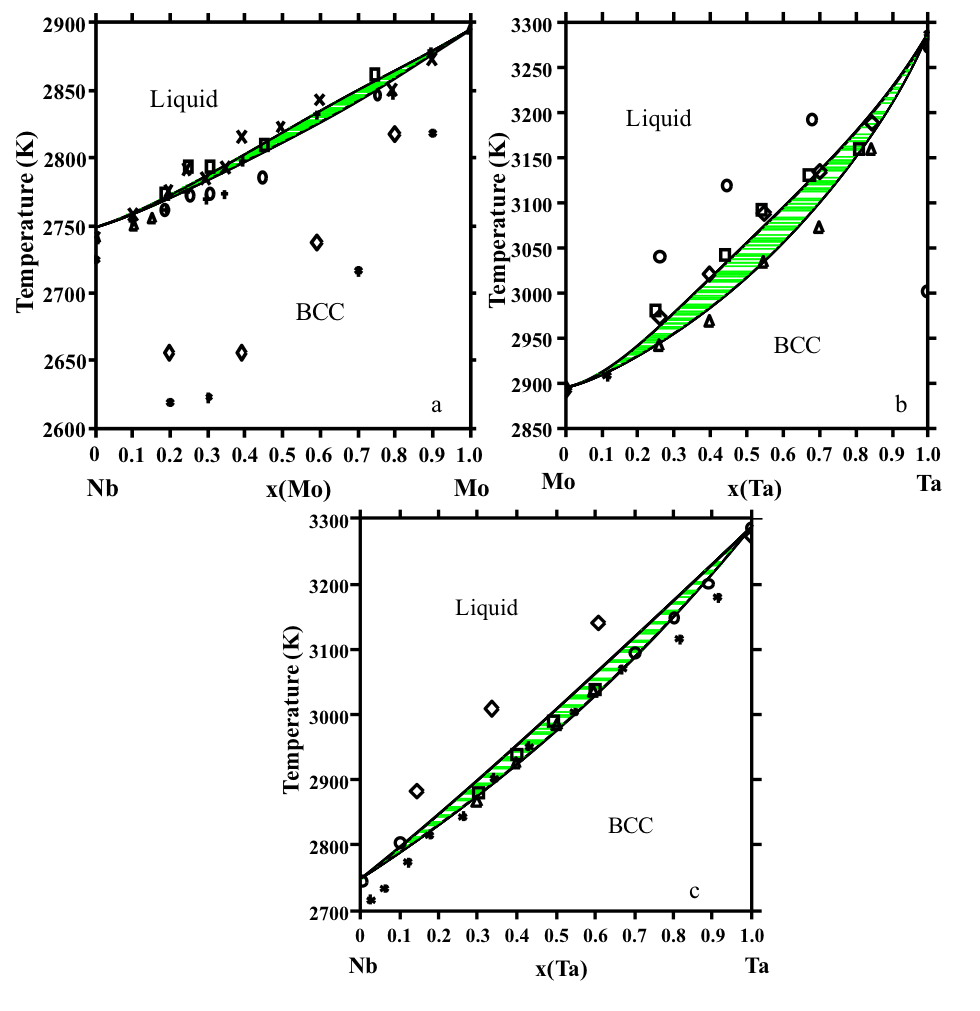
\includegraphics[width=\textwidth]{Chapter-3/Figures/binary1.png}
	\caption{Previously modeled thermodynamic descriptions of the Mo-Nb (a) \cite{Xiong2004}, Mo-Ta (b) \cite{Xiong2004} and Nb-Ta (c) \cite{Xiong2004} binary systems in comparison with available liquidus and solidus phase boundary experimental data to ensure accuracy (as detailed in \cite{Xiong2004}). }
	\label{Ch3-figure:binary1}
\end{figure}
%%%

\newpage
%%%
\begin{figure}[H]
	\centering
	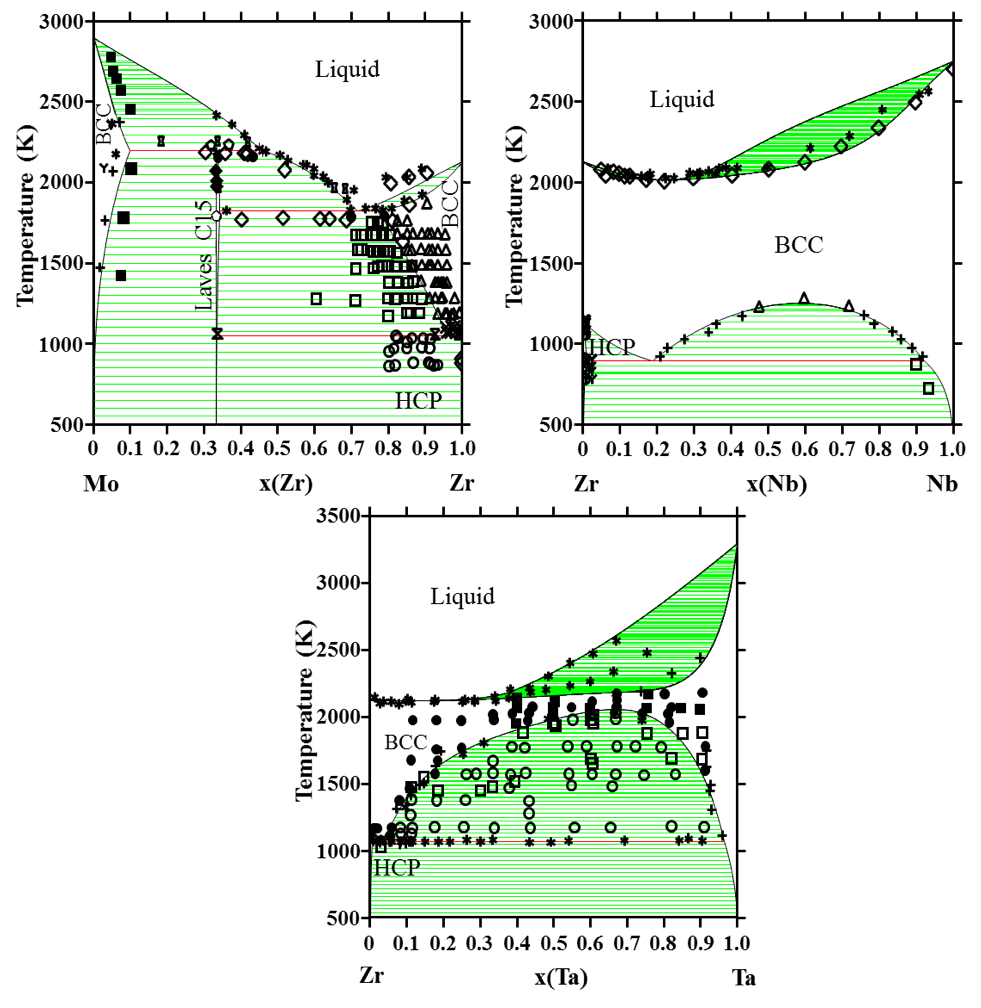
\includegraphics[width=\textwidth]{Chapter-3/Figures/binary2.png}
	\caption{Previously modeled thermodynamic description of the Mo-Zr \cite{Perez2003} system is plotted with phase boundary, reaction, single phase and two phase experimental data. The previously modeled Nb-Zr \cite{Guillermet1991,Abriata1982} system is plotted with solidus, hcp solvus and bcc solvus experimental data. The previously modeled Ta-Zr \cite{Guillermet1995} system is plotted with single-phase, two-phase, phase boundary and solidus experimental data (detailed in the mentioned references).}
	\label{Ch3-figure:binary2}
\end{figure}
%%%

\newpage
%%%
\begin{figure}[H]
	\centering
	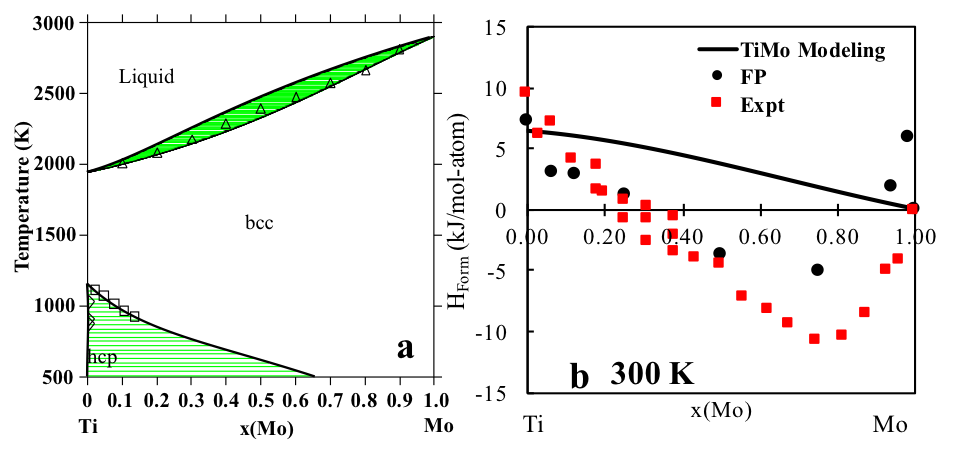
\includegraphics[width=\textwidth]{Chapter-3/Figures/TiMo.png}
	\caption{Previously modeled thermodynamic description of the Ti-Mo system versus available phase boundary and solidus experimental data to ensure accuracy \cite{Ansara1998,Murray1981} (a), and enthalpy of formation of the bcc phase predicted by the previous thermodynamic modeling (solid line) at 300 K versus the present first-principles calculations (circles) at 0 K and compared with the enthalpy of formation of the bcc phase obtained from experiments (square) \cite{Uesugi2013} (b).}
	\label{Ch3-figure:TiMo}
\end{figure}
%%%

\newpage
%%%
\begin{figure}[H]
	\centering
	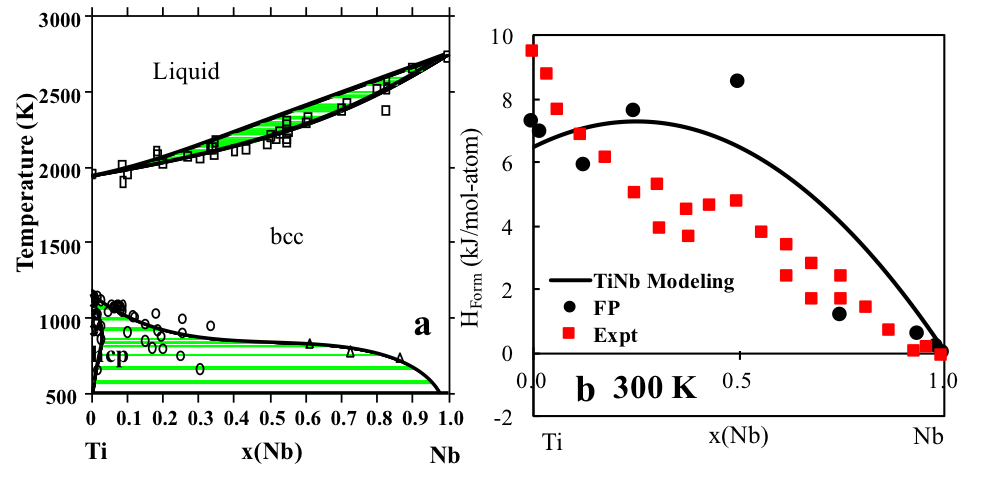
\includegraphics[width=\textwidth]{Chapter-3/Figures/TiNb.png}
	\caption{Previously modeled thermodynamic description of the Ti-Nb system versus available phase boundary and solidus experimental data to ensure accuracy \cite{Zhang2001,Kumar1994,Kumar1994a}[20,48] (a), and enthalpy of formation of the bcc phase predicted by the previous thermodynamic modeling (solid line) at 300 K versus the present first-principles calculations (circles) at 0 K compared with the enthalpy of formation of the bcc phase obtained from experiments (square) \cite{Uesugi2013} (b).}
	\label{Ch3-figure:TiNb}
\end{figure}
%%%

\newpage
%%%
\begin{figure}[H]
	\centering
	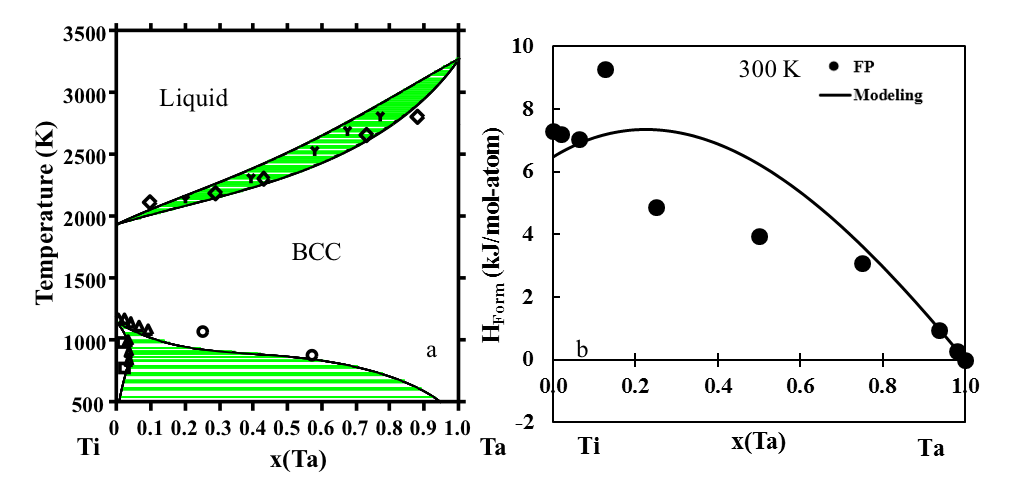
\includegraphics[width=\textwidth]{Chapter-3/Figures/TiTa.png}
	\caption{Previously modeled thermodynamic description of the Ti-Ta system versus available phase boundary and solidus experimental data to ensure accuracy \cite{Murray1987,Ansara1998} (a), and enthalpy of formation of the bcc phase predicted by the previous thermodynamic modeling (solid line) at 300 K versus the present first-principles calculations (circles) at 0 K (b).}
	\label{Ch3-figure:TiTa}
\end{figure}
%%%

\newpage
%%%
\begin{figure}[H]
	\centering
	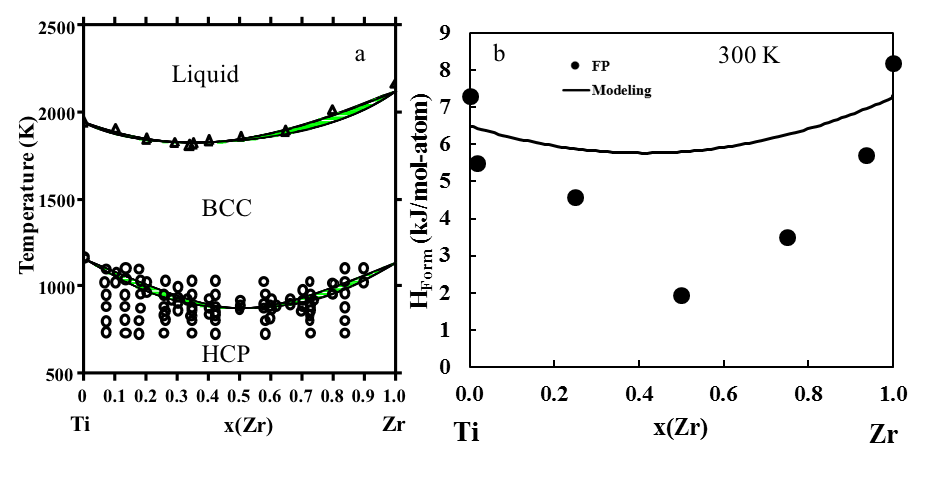
\includegraphics[width=\textwidth]{Chapter-3/Figures/TiZr.png}
	\caption{Previously modeled thermodynamic description of the Ti-Zr system versus available phase boundary and solidus experimental data to ensure accuracy \cite{Kumar1994a} (a), and enthalpy of formation of the bcc phase predicted by the previous thermodynamic modeling (solid line) at 300 K versus the present first-principles calculations (circles) at 0 K (b).}
	\label{Ch3-figure:TiZr}
\end{figure}
%%%

\newpage
%%%
\begin{figure}[H]
	\centering
	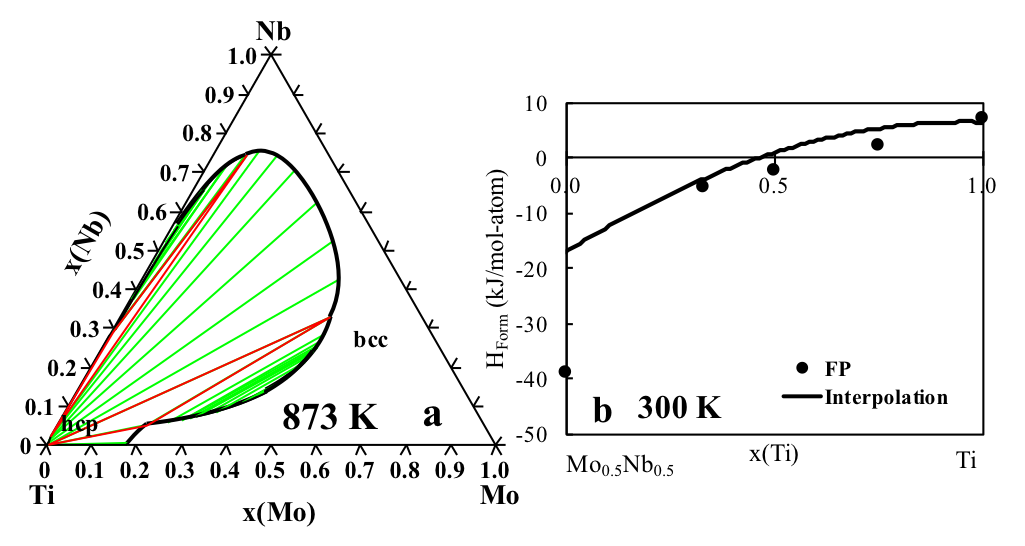
\includegraphics[width=\textwidth]{Chapter-3/Figures/TiMoNb.png}
	\caption{Binary interpolation of the isothermal section of the Ti-Mo-Nb system plotted at 873 K (a), and enthalpy of formation of the bcc phase predicted by the binary interpolation of the thermodynamic modeling (solid line) at 300 K versus the present first-principles calculations (circles) at 0 K (b).}
	\label{Ch3-figure:TiMoNb}
\end{figure}
%%%

\newpage
%%%
\begin{figure}[H]
	\centering
	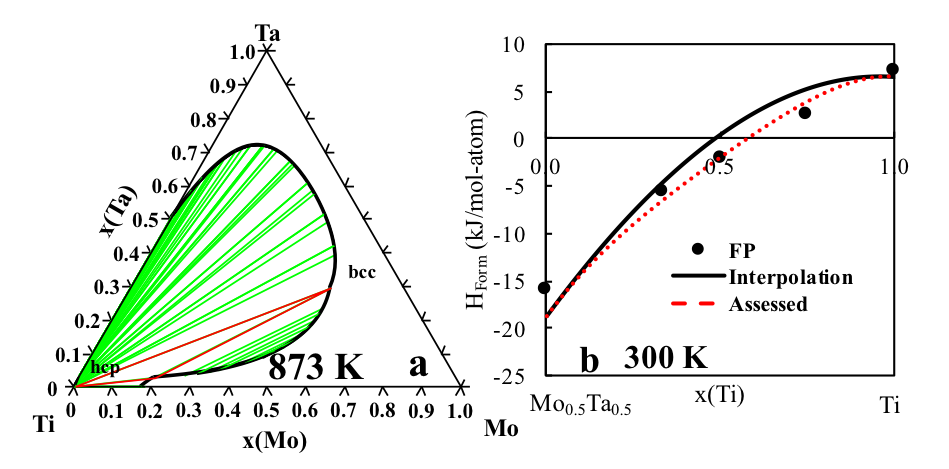
\includegraphics[width=\textwidth]{Chapter-3/Figures/TiMoTa1.png}
	\caption{Binary interpolation of the isothermal section of the Ti-Mo-Ta system plotted at 873 K (a), and enthalpy of formation of the bcc phase predicted by the previous thermodynamic modeling (solid line) at 300 K and the ternary assessed thermodynamic modeling (red dotted line) versus the present first-principles calculations (circles) at 0 K (b).}
	\label{Ch3-figure:TiMoTa1}
\end{figure}
%%%

\newpage
%%%
\begin{figure}[H]
	\centering
	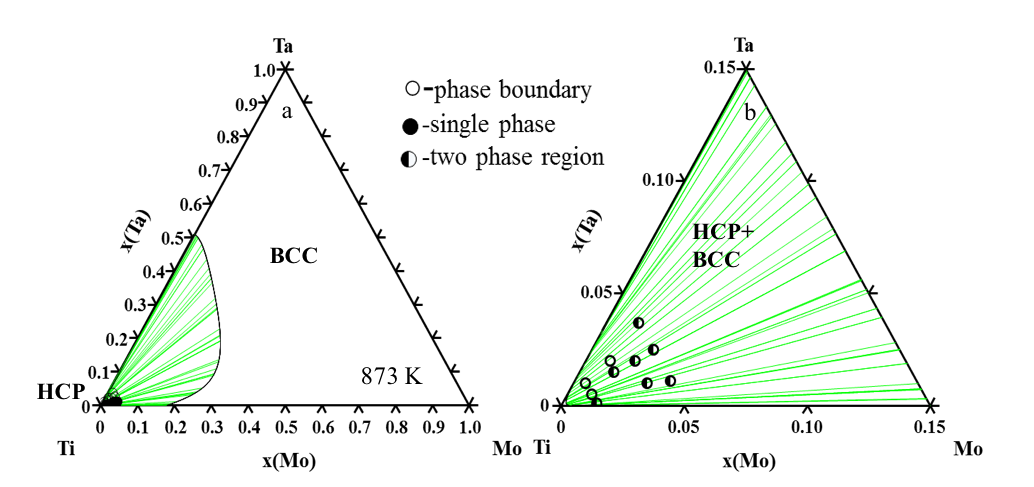
\includegraphics[width=\textwidth]{Chapter-3/Figures/TiMoTa2.png}
	\caption{Ternary assessed isothermal section of the Ti-Mo-Ta system plotted at 873 K (a), and zoomed in ternary assessed isothermal section at 873 K (b) with the phase boundary and two-phase region experimental data \cite{Nikitin1971} to ensure accuracy of the ternary assessment.}
	\label{Ch3-figure:TiMoTa2}
\end{figure}
%%%

\newpage
%%%
\begin{figure}[H]
	\centering
	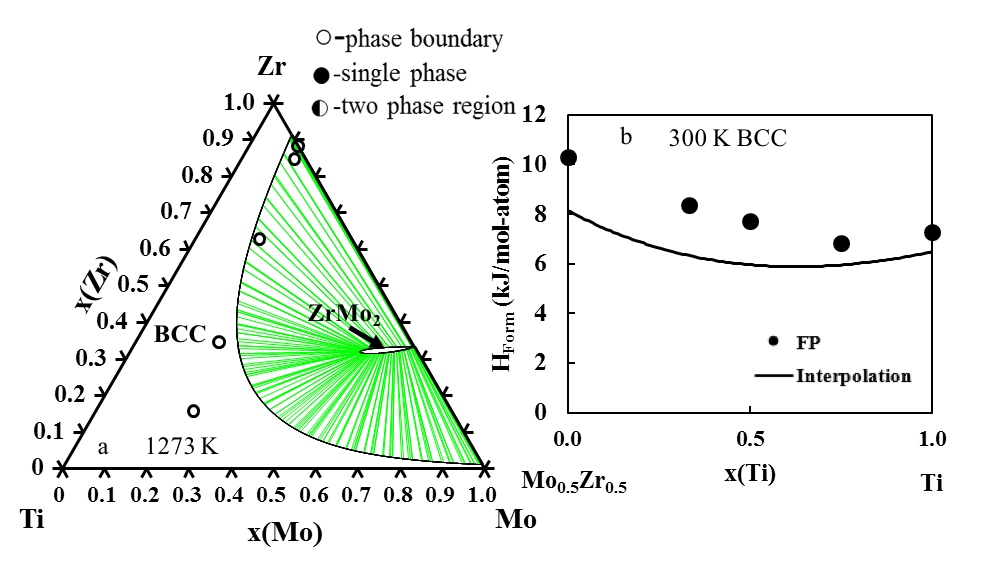
\includegraphics[width=\textwidth]{Chapter-3/Figures/TiMoZr.png}
	\caption{The assessed ternary isothermal section of the Ti-Mo-Zr system plotted at 1273 K compared with experimental phase boundary data \cite{Kar2008,Prokoshkin1967} (a), and enthalpy of formation of the bcc phase predicted by the previous thermodynamic modeling (solid line) at 300 K versus the present first-principles calculations (circles) at 0 K (b).}
	\label{Ch3-figure:TiMoZr}
\end{figure}
%%%

\newpage
%%%
\begin{figure}[H]
	\centering
	\includegraphics[width=\textwidth]{Chapter-3/Figures/TiNbTa1.png}
	\caption{Binary interpolation of the isothermal section of the Ti-Nb-Ta system plotted at 673 K compared with experimental phase boundary data \cite{Na2001} (a), and binary interpolation of the isothermal section of the Ti-Nb-Ta system plotted at 823 K compared with experimental phase boundary data \cite{Na2001} (b).}
	\label{Ch3-figure:TiNbTa1}
\end{figure}
%%%

\newpage
%%%
\begin{figure}[H]
	\centering
	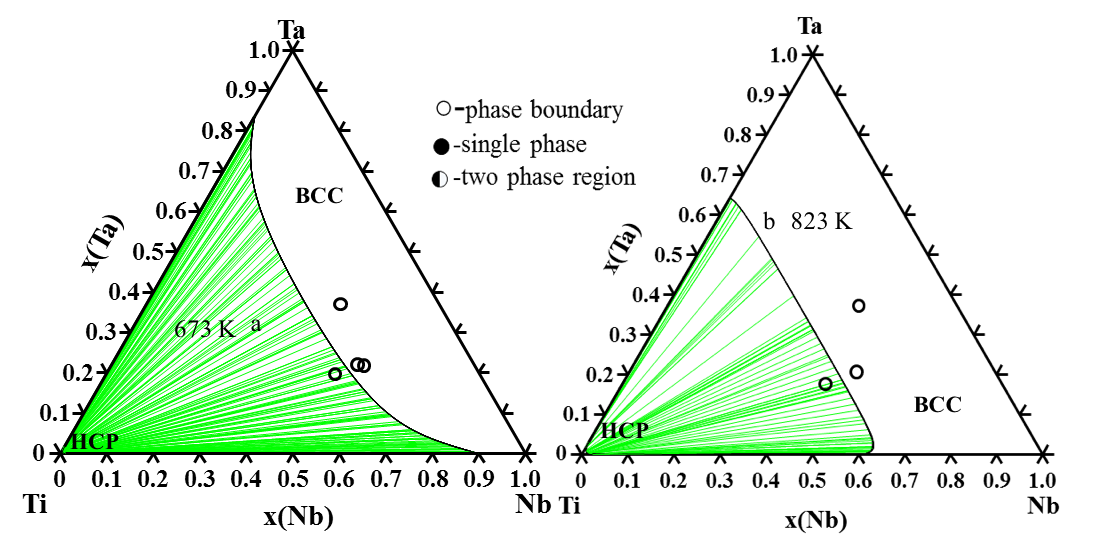
\includegraphics{Chapter-3/Figures/TiNbTa2.png}
	\caption{Enthalpy of formation of the bcc phase predicted by the previous thermodynamic modeling (solid line) at 300 K and the ternary assessed thermodynamic modeling (red dotted line) versus the present first-principles calculations (circles) at 0 K.}
	\label{Ch3-figure:TiNbTa2}
\end{figure}
%%%

\newpage
%%%
\begin{figure}[H]
	\centering
	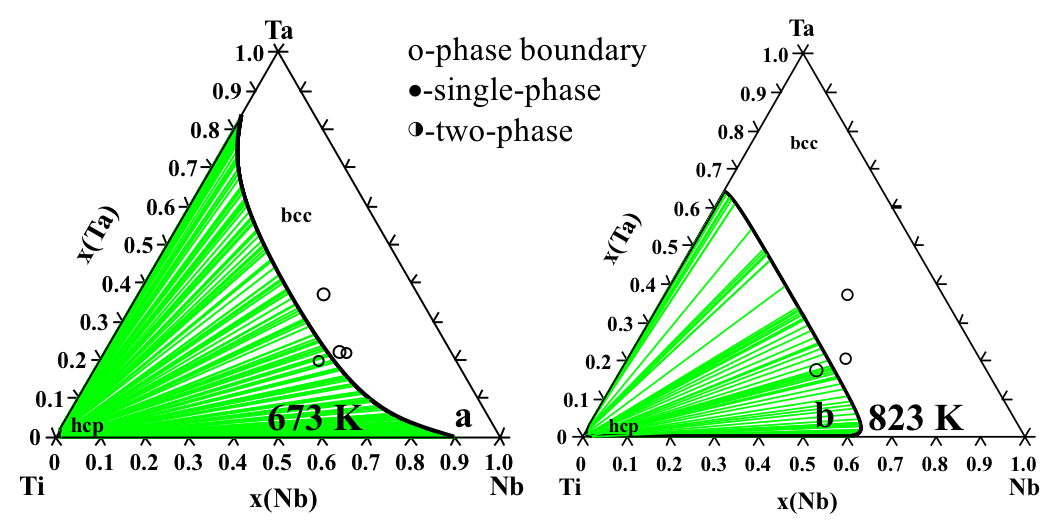
\includegraphics[width=\textwidth]{Chapter-3/Figures/TiNbTa3.png}
	\caption{Ternary assessed isothermal section of the Ti-Nb-Ta system plotted at 673 K compared with experimental phase boundary data \cite{Na2001} to ensure accuracy of the ternary assessment (a), and ternary assessed isothermal section at 823 K compared with experimental phase boundary data \cite{Na2001} to ensure accuracy of the ternary assessment (b).}
	\label{Ch3-figure:TiNbTa3}
\end{figure}
%%%

\newpage
%%%
\begin{figure}[H]
	\centering
	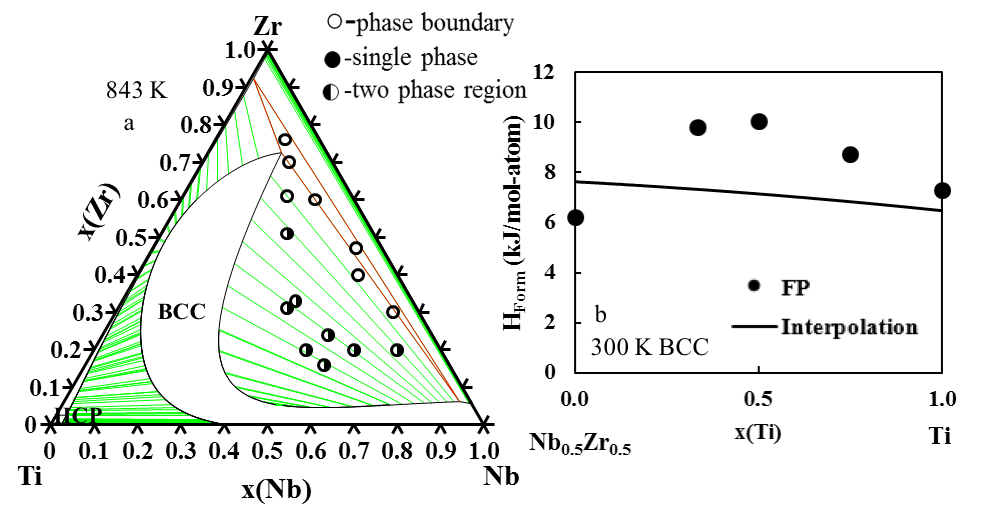
\includegraphics[width=\textwidth]{Chapter-3/Figures/TiNbZr.png}
	\caption{Binary interpolation of the isothermal section of the Ti-Nb-Zr system plotted at 843 K compared with experimental phase boundary and two-phase region data \cite{Tokunaga2007} (a), and enthalpy of formation of the bcc phase predicted by the previous thermodynamic modeling (solid line) at 300 K versus the present first-principles calculations (circles) at 0 K (b).}
	\label{Ch3-figure:TiNbZr}
\end{figure}
%%%

\newpage
%%%
\begin{figure}[H]
	\centering
	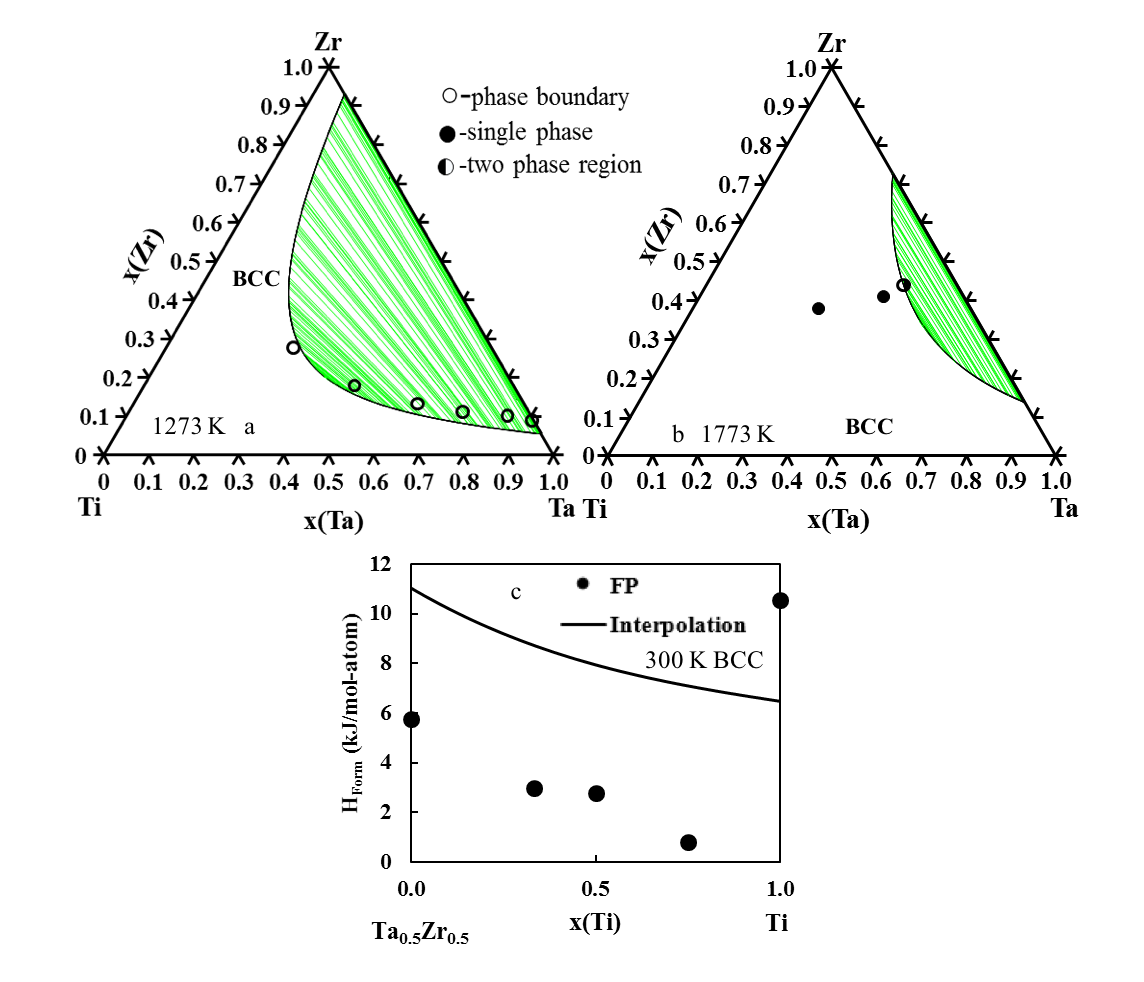
\includegraphics[width=\textwidth]{Chapter-3/Figures/TiTaZr1.png}
	\caption{Binary interpolation of the isothermal section of the Ti-Ta-Zr system plotted at 1273 K compared with experimental phase boundary data \cite{Lin1996,Hoch1964} (a), and binary interpolation of the isothermal section of the Ti-Ta-Zr system plotted at 1773 K compared with experimental single phase and two-phase region data \cite{Lin1996,Hoch1964} (b).}
	\label{Ch3-figure:TiTaZr1}
\end{figure}
%%%

\newpage
%%%
\begin{figure}[H]
	\centering
	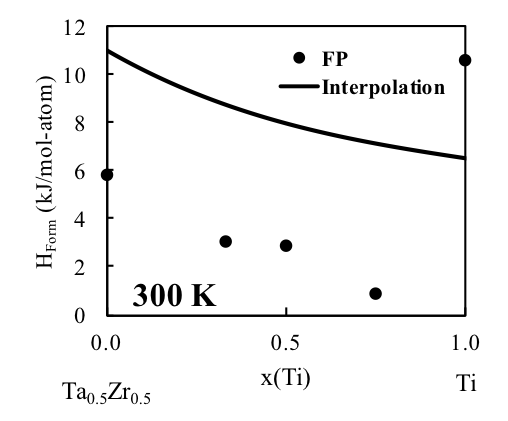
\includegraphics{Chapter-3/Figures/TiTaZr2.png}
	\caption{Enthalpy of formation of the bcc phase predicted by the previous thermodynamic modeling (solid line) at 300 K versus the present first-principles calculations (circles) at 0 K.}
	\label{Ch3-figure:TiTaZr2}
\end{figure}
\chapter{First-principles aided thermodynamic modeling of the Sn-Ta system}

\section{Introduction}

Currently, the biomaterial implant research of Ti alloys is focused on biocompatible elements that stabilize the body centered cubic (bcc, $\beta$) phase of Ti and help to lower its elastic modulus. Tantalum (Ta) is a biocompatible element and is considered to be a strong -stabilizers \cite{Brailovski2011b}. Recently, tin (Sn) has also been researched for use in Ti-alloys due to its biocompatibility and low cost \cite{Niinomi2012}. Kuroba et al. \cite{Kuroda1998} studied various Ti-alloys such as Ti-29-Nb-13Ta-2Sn (weight percentage, and similarly hereinafter unless specified otherwise), Ti-29Nb-13Ta-4Mo, and Ti-29Nb-13Ta-6Sn for use as biocompatible implant materials. Kuroba and Hagiwara \cite{He2004} also studied new Ti-Cu-Ni-Sn-Ta alloys for the artificial materials used in orthopedic surgeries. The Sn-Ta system is thus an important sub-system for this purpose \cite{He2006}.  A complete knowledge base of the thermodynamic description of Sn-Ta can be used to examine the effects of temperature and composition on phase stability for higher order systems and help to tailor experimental alloy selections to viable options. The CALPHAD technique, in combination with first-principles and phonon calculations based on the DFT, has been proven to provide valuable data to model the thermodynamic properties of binary such as Ta-Sn that lack sufficient experimental data \cite{Liu2009}. The Sn-Ta system has three solid solution phases and two intermetallic compounds, i.e. the bcc, body centered tetragonal (bct), and diamond solution phases, and the intermetallic compounds Ta$_{3}$Sn with space group $Pm\overline{3}n$ and TaSn$_{2}$ (Ta$_{1.2}$Sn$_{1.8}$) with space group $Fddd$ \cite{Okamoto2003}.

 In the present work, thermodynamic data was predicted using first-principles calculations for the two intermetallics and for the bcc, bct and diamond solution phases. The finite temperature properties of the phases were obtained using the Debye-Gr\"uneisen model \cite{Shang2010} and phonon calculations based on the supercell approach \cite{Wang2012}.  The DFT data was used to model the parameters of the Gibbs energy of each phase using the CALPHAD technique.

\section{Literature Review}

The Sn-Ta binary system was studied by Okamoto \cite{Okamoto2003}, Studnitzky and Schmid-Fetzer \cite{Studnitzky2002}, and Basile \cite{Basile1971}.  Both of the intermetallic phases, Ta$_{3}$Sn and TaSn$_{2}$, were shown to have a very narrow homogeneity range. Basile \cite{Basile1971} observed that TaSn$_{2}$ is located around Ta$_{1.2}$Sn$_{1.8}$ which was then designated as Ta$_2$Sn$_3$ by Okamoto \cite{Okamoto2003}. It seems that TaSn$_2$ is a more compatible description of the stoichiometric compound based on the descriptions of similar systems (V-Sn, and Nb-Sn) \cite{Yue2009,Toffolon1998,Toffolon2002}, and thus will be used in the present work. Basile \cite{Basile1971} determined TaSn$_2$ has a peritectic reaction at 595 $^{\circ}$C and used X-ray diffraction (XRD) to elucidate the lattice parameters of TaSn$_2$.  

Studnitzky and Schmid-Fetzer \cite{Studnitzky2002} used powder samples to study the Ta$_3$Sn intermetallic phase and verified the results previously reported by Basile \cite{Basile1971}. They cold pressed the pure element powders at 600 MPa and then heated the pellets at 1000 $^{\circ}$C for up to 48 hours.  The resulting pellet was then cold pressed at 600 MPa again. Under these conditions TaSn$4_2$ was observed at 400 $^{\circ}$C, but was not present as the temperature increased to 600 $^{\circ}$C.  In the work by Courtney et al. \cite{Courtney1965}, Ta$_3$Sn was studied to see how the temperature affects the long-range ordering parameter. In Courtney et al.'s work, Ta$_3$Sn powder samples were sintered at 600, 700, 950, 1200, and 1450 $^{\circ}$C for 2, 4, 7, and 16 days, respectively.  Each sample was then studied using XRD at room temperature to examine the phases present and the long-range ordering. They concluded that the transition temperature of superconductivity for Ta$_3$Sn varied by a maximum of 4 $^{\circ}$K based on heat treatment and sintering times due to long-range ordering that occurred. Courtney et al. also measured the lattice parameter of each sample and reported the average value of this cubic phase being 5.285 $\AA$.


\section{Modeling and Calculations}

\subsection{First-principles details}

In the present work, the Vienna ab-initio Simulation Package (VASP) was used to perform the first-principles calculations \cite{Kresse1996}. The projector augmented-wave (PAW) \cite{Kresse1999,Blochl1994} method was used to describe the electron-ion interactions. Based on the work of comparing X-C functionals (Figure \ref{Ch2-figure:PBEvsPW91}) the exchange-correlation functional of the generalized gradient approach depicted by Perdew, Burke, and Ernzerhof (PBE) was employed \cite{Perdew1996a}. A sigma value of 0.2 eV and a plane wave energy cutoff of 1.3 times higher than the highest default cutoff was adopted. The Brillouin zone sampling was done with Bl$\ddot{o}$chl corrections \cite{Blochl1994} using a gamma centered Monkhorst-Pack (MP) scheme \cite{Monkhorst1976a}. The k-points grid for diamond$\-$Sn, bcc-Ta, TaSn$_2$, and bcc-Sn were 4x4x4, 6x6x6, 10x10x5, and 6x6x6 respectively. The k-point grids for the bct-Sn, Ta$_3$Sn and bcc SQS calculations used an automated k-point mesh generator in VASP with the length of the subdivisions specified as 80. The energy convergence criterion of the electronic self-consistency is set as $10^{-4}$ eV/atom and $10^{-4}$ eV/A was set as the stopping criteria for the ionic relaxation loop for all of the calculations. 

To calculate the enthalpy of formation of the bcc phase across the entire composition range, the enthalpy of formation of Ta and Sn in the bcc phase were calculated with five different compositions of Ta$_{1-x}$Sn$_{x}$, where x=0.0185 (Ta$_{53}$Sn, 54 atoms), 0.25, 0.5, 0.75, and 0.9815 (TaSn$_{53}$, 54 atoms). For x=0.0185 and 0.9815, calculations were performed on a diluted 54 atom cell where all atoms but one was Sn or Ta (Ta$_{53}$Sn and TaSn$_{53}$). For x=0.25, 0.5, and 0.75, 16-atom special quasirandom structures (SQS) in the bcc phase developed by Jiang et al. \cite{Jiang2004} were used to mimic the behavior of random structures. The relaxation of these structures is complicated and discussed in the methodology section. The enthalpy of formation was plotted as a function of composition and then used for the modeling.  

\subsection{CALPHAD}

The Gibbs energy functions of pure elements were adopted from the SGTE (SSUB) database \cite{Dinsdale1991}. In the present work, the bcc and liquid phases were modeled in conjunction with the two intermetallics Ta$_3$Sn and TaSn$_2$. Dilute first-principles calculations of Ta in Sn were done for the diamond and bct phases. However, there is little solubility of Ta in these phases and there is no description of pure Ta in these phases available in SGTE. So, no binary interaction parameters were introduced in the modeling similar to other Sn systems such as Nb-Sn and V-Sn \cite{Yue2009,Toffolon2002}. The energy of the liquid and bcc solution phases were modeled using Eq. \ref{eq: gibbssolution} and \ref{eq: gibbexsol}, while Ta$_3$Sn and TaSn$_2$ were modeled according to Eq. \ref{eq: stoichiometric}.

\section{Results and discussion}

\subsection{First-principles}

To evaluate the accuracy of phonon calculations for the present system, both the dispersion curves and the phonon DOS are plotted for bcc-Ta, bct-Sn, TaSn$_2$, and Ta$_3$Sn in Figure \ref{Ch4-figure:Taphonon},  Figure \ref{Ch4-figure:Snphonon}, Figure \ref{Ch4-figure:TaSn2phonon}, and Figure \ref{Ch4-figure:Ta3Snphonon}, respectively.  The bcc-Ta phonon dispersion curve in  Figure \ref{Ch4-figure:Taphonon} is compared with values obtained by Taioli et al. \cite{Taioli2007a} using neutron scattering, showing good agreement. The longitudinal modes (LO) and the transverse modes (TO) measured by Raman spectroscopy \cite{Olijnyk1992} (open square) along with the previous theoretical predictions at the M point (filled square) for bct-Sn are compared with the calculated phonon dispersion curve in Figure \ref{Ch4-figure:Snphonon}. The substantial difference for the LO mode may be due to the temperature and pressure differences as pointed out by Olijnyk \cite{Olijnyk1992}. No imaginary phonon frequencies are obtained in the phonon DOS plots for bcc-Ta, bct-Sn, TaSn$_2$, Ta$_3$Sn, indicating that they are all mechanically and dynamically stable at 0 $^\circ$K. 

The calculated lattice parameters at 0 $^\circ$K from the EOS fitting and with the Debye and phonon models at 298 $^\circ$K are compared to available experimental and previous DFT results in Table \ref{Ch4-table:TaSnlattice}. The lattice parameters of Ta are compared with the experimental lattice parameters by Predmore and Arsenault \cite{Predmore1970} at room temperature and the previous 0 $^\circ$K DFT results by Shang et al. \cite{Shang2010b} who used the GGA-PW91 exchange correlation functional. The Sn lattice parameters are compared to experimental work by Allen et al. \cite{Allen1991} at 298 $^\circ$K and calculations by Arr$\acute{o}$yave et al. \cite{Arroyave2006a}. The properties of the TaSn$_2$ and Ta$_3$Sn intermetallics have not been calculated previously and are compared to experimental values by Calvert et al. \cite{Calvert1991} and Courtney et al. \cite{Courtney1965}, respectively. The results show a less than 0.5$\%$ difference when compared with other DFT results at 0 $^\circ$K. There is a less than 2$\%$ difference between the DFT 0 $^\circ$K results and the experiments, which are listed in Table \ref{Ch4-table:TaSnlattice}. The variance is due to the fact that the calculations are at 0 $^\circ$K and the experiments are at a higher temperature. When comparing the calculated lattice parameters at 298 $^\circ$K to the experiments, all of the predictions improve to show a less than 1$\%$ difference with the exception of Sn, which shows a less than 2$\%$ difference. 

Table \ref{Ch4-table:TaSnvolume} shows the equilibrium volume, $V_{0}$, bulk modulus, $B_{EOS}$, and the derivative of bulk modulus $B'_{EOS}$ obtained by the EOS E-V fitting of the first-principles data at 0 $^\circ$K.  The Sn and Ta calculations are compared with previous first-principles calculations and available experiments. The volume shows a less than 0.5$\%$ difference between the previous DFT results and current DFT results for both Sn and Ta \cite{Predmore1970,PeltzeryBlanca1993a}. The comparison of the DFT results at 0 $^\circ$K and the experimental results at 298 K for volume show a slightly higher variance of less than 5 $\%$ due to the different in temperature \cite{Shang2010b,PeltzeryBlanca1993a}. The $B_{EOS}$ comparison of previous 0 $^\circ$K DFT results and the present 0 $^\circ$K DFT results show a less than 7 GPa difference and the DFT results at 0 $^\circ$K vary by less than 11 GPa from the experimental results at 298 $^\circ$K \cite{Predmore1970,Shang2010b,PeltzeryBlanca1993a}. The difference between the current calculations and the previous values may be due to many reasons; e.g. the different choices in input parameters used by Peltzer et al. \cite{PeltzeryBlanca1993a} and different exchange correlation functionals. Another reason is due to the temperature difference 0 $^\circ$K (calculations) versus 298 $^\circ$K (experiments). Figure \ref{Ch4-figure:Tafinitetemp} shows the enthalpy and entropy of Ta from the Debye and phonon approaches in comparison with the data from the SGTE pure element database \cite{Dinsdale1991}. Figure \ref{Ch4-figure:Snfinitetemp} shows the comparison of the enthalpy and entropy calculated for Sn from the phonon and Debye model to the SGTE pure element database \cite{Dinsdale1991}. Both show excellent agreement.

The elastic stiffness constants and polycrystalline elastic properties calculated by the Hill approach and the scaling factors for the Debye model are shown in Table \ref{Ch4-table:TaSnelastic}. To ensure the accuracy of the scaling factor, the elastic stiffness constants and moduli are compared with previous first-principles results \cite{Jouault1967_611,Bergerhoff1983,Geller1955_165,Karlsruhe,MaterialsProject}. The previous calculation results and present calculation results only vary slightly for the TaSn$_2$ structure. The present work calculated the elastic stiffness constants for the Ta$_3$Sn structure at 2 different atom sizes and compared the results with previous calculations by the Materials Project \cite{Jouault1967_611,Bergerhoff1983,Geller1955_165,Karlsruhe,MaterialsProject}. The present elastic stiffness results are quite similar. There is a larger variance between the present results and the Materials Project results. This can be attributed to the different input parameters and exchange correlation functional used (PBE in the present work and GGA-PW91 in Materials Project). $B$ calculated from the $c_{ij}$ methodology is compared with the $B)_{EOS}$ obtained from the EOS fitting, showing a difference of less than 3$\%$. Since the $B_{EOS}$ from the EOS fitting is already compared to experiments, the elastic calculations and the scaling factor for the Debye model are thus deemed accurate.

\subsection{CALPHAD}

The PARROT module in the Thermo-Calc software \cite{Andersson2002} is used to optimize the parameters of the Gibbs energy function of the TaSn$_2$ and Ta$_3$Sn intermetallics as well as the binary interaction parameters for the bcc and liquid phases. The Gibbs energy parameters of the intermetallics are first estimated from the thermodynamic properties obtained by the phonon supercell method because the phonon calculations are regarded as more accurate than the Debye model. While the decomposition temperature of the TaSn$_2$intermetallic is known to be 868 $^\circ$K from experiments, the decomposition of the Ta$_3$Sn intermetallic has not been reported in the literature. It is noted that both the Nb-Sn and V-Sn systems, which are quite similar to the Ta-Sn system, have the X$_3$Sn phase forming through a peritectic reaction of bcc+Liquid$\rightarrow$X$_3$Sn \cite{Yue2009,Toffolon2002,Toffolon1998}. Based on the assumption from similar works that Ta$_3$Sn is also formed through a peritectic reaction, the Ta$_3$Sn parameters are adjusted and the parameters for the liquid phase are evaluated. The evaluation of the Gibbs parameters along with the results from the Debye model and the phonon quasiharmonic approach for TaSn$_2$ and Ta$_3$Sn are plotted in Figure \ref{Ch4-figure:TaSn2finitetemp} and Figure \ref{Ch4-figure:Ta3Snfinitetemp}, respectively. As seen in both figures, the data from the phonon method correlates well with the current CALPHAD modeling. This is to be expected since this data was used to evaluate the parameters. It is noted in Figure \ref{Ch4-figure:TaSn2finitetemp}, that the heat capacity and entropy of TaSn$_2$ from the current CALPHAD modeling is higher than those from the first-principles calculations. This is due to the fact that the enthalpy and entropy values from DFT were adjusted with the experimental data of the peritectic temperature.

The bct and diamond phases are treated as ideal due to the little solubility. As previously stated, the enthalpies of formation of the bcc phase for five different Sn-Ta compositions are calculated and plotted in Figure \ref{Ch4-figure:HofForm}, showing asymmetrical behavior. There is a discrepancy between the first-principles value and the CALPHAD modeling for the lattice stability of bcc-Sn. The first-principles predicts a value of 15.48 kJ/mol-atom and the CALPHAD model gives 4.42 kJ/mol-atom. This difference is expected to be due to the instability of Sn in the bcc phase. Wang et al. \cite{Wang2004a} concluded and discussed the same discrepancy when comparing first-principles DFT results to SGTE data for Os and Ru. Wang et al. calculated the lattice stability of bcc and fcc (face centered cubic) structure for Os and Ru, both stable in the hexagonal close packed phase at standard temperature and pressure, and concluded a difference of approximately 40 and 60 kJ/mol for Ru and Os, respectively. Wang et al. attributed this difference to the fact that when using first-principles calculations of unstable structures, frequencies of some of the phonon modes would become imaginary and thus the results would be less accurate. On the other hand, the CALPHAD technique can extrapolate lattice stabilities from binary solutions for which an alloying element has stabilized the otherwise unstable structure. These enthalpies of formation calculated from the SQS first-principles calculations are used to evaluate the bcc binary interaction parameters in the present CALPHAD modeling. The enthalpy of formation of the bcc phase is negative at the Ta rich side and becomes positive at the Sn rich side. This is common for X-Sn systems \cite{Yue2009,Toffolon2002}, such as the Nb-Sn system \cite{Toffolon2002} shown in Figure \ref{Ch4-figure:HofForm}. It should be noted that Toffolon et al. \cite{Toffolon1998,Toffolon2002} used experimental data on the Sn-rich bcc phase to evaluate the Nb-Sn system's bcc interaction parameters. Due to the asymmetry of enthalpy of formation for the bcc phase, a subregular $^1$L interaction parameters is introduced. 

The interaction parameters obtained in the present work are listed in Table \ref{Ch4-table:ip}. Based on these model parameters, the phase diagram is calculated and shown in Figure \ref{Ch4-figure:SnTaPD}. The melting temperature of Ta$_3$Sn is predicted to be 2884 $^\circ$K. Both the intermetallics decompose incongruently similar to those in the Nb-Sn and V-Sn systems. As seen in Table \ref{Ch4-table:ip}, both intermetallic phases have a negative enthalpy of formation and a negative entropy of formation. This goes along with previous predictions by Arroyave and Liu \cite{Arroyave2006} where they showed that the enthalpy and entropy of formation have the same sign. The calculated enthalpy of mixing of the liquid phase is plotted in Figure \ref{Ch4-figure:HofMix}. The interaction parameter for the liquid phase allows for an accurate representation of the phase stability in Figure \ref{Ch4-figure:SnTaPD} but may need to be slightly adjusted if experimental data would come available.

\section{Conclusion}

The present work incorporates the thermodynamic data from DFT-based first-principles calculations and the available experimental data in the literature to model the Gibbs energies for the bcc and liquid solution phases and the stoichiometric Ta$_3$Sn and TaSn$_2$ phases of the Sn-Ta system.  First-principles calculations are used to predict the enthalpy of formation of the bcc phase for the evaluation of interaction parameters in the phase. The decomposition temperature of Ta$_3$Sn is predicted to be 2884 $^\circ$K. The completed thermodynamic description is complied into a tdb file. The tdb file and raw data from the first-principles calculations are in appendix b.

\newpage
\begin{table}[H]
	\caption{Lattice parameters from first-principles calculations compared with experimental values.}
	\centering
	\begin{tabular}{ c c c c c c }
		\hline
		Phase & Space Group & $a$ ($\AA$) & $b$ ($\AA$)  & $c$ ($\AA$) & Reference\\
		\hline
		bcc-Ta & Im$\overline{3}$m & 3.316 & & &This work (0 $^\circ$K)\\
		            &                             & 3.328 & & & This work phonon (298 $^\circ$K)\\
		            &                             & 3.330 & & & This work Debye (298 $^\circ$K)\\
		            &                             & 3.30   & & & Expt. \cite{Predmore1970}\\
		            &                             & 3.32   & & & DFT (0 $^\circ$K) \cite{Shang2010b}\\
		bct-Sn & I4$_1$/amd & 5.939 & & 3.214 & This work (0 $^\circ$K)\\
		            &                   & 5.959 & & 3.236 & This work phonon (298 $^\circ$K)\\
		            &                   & 5.954 & & 3.222 & This work Debye (298 $^\circ$K)\\
		            &                   & 5.83   & & 3.18 & Expt. \cite{Allen1991}\\
		            &                   & 5.93   & & 3.23 & DFT (0 $^\circ$K) \cite{Arroyave2006a}\\
         TaSn$_2$ & Fddd & 5.641 & 9.766 & 19.200 & This work (0 $^\circ$K)\\
              &          & 5.652 & 9.786 & 19.238 & This work phonon (298 $^\circ$K)\\
              &          & 5.652 & 9.785 & 19.238 & This work Debye (298 $^\circ$K)\\
                         &          & 5.63 & 9.80 & 19.18 & Expt. \cite{Calvert1991}\\
          Ta$_3$Sn & Pm$\overline{3}$n & 5.304 & & &This work (0 $^\circ$K)\\
                          &                   & 5.319 & & & This  work phonon (298 $^\circ$K)\\
                          &                   & 5.319 & & & This work Debye (298 $^\circ$K)\\
                          &                   & 5.29 & & & Expt. \cite{Courtney1965}\\
		\hline
	\end{tabular}
	\label{Ch4-table:TaSnlattice}
\end{table}
\clearpage
%%%

\newpage
\begin{table}[H]
	\caption{Equilibrium volume $V_{0}$, bulk modulus $B_{EOS}$, and the first derivative of bulk modulus with respect to pressure $B'_{EOS}$, from fitted equilibrium properties from the EOS at 0 $^\circ$K compared to experimental work and previous DFT studies.}
	\centering
	\begin{tabular}{ c c c c c }
		\hline
		Phase & $V_{0}$ ($\AA^3$/atom) & $B_{EOS}$ (GPa) & $B'_{EOS}$ & Reference\\
		\hline
		bcc-Ta & 18.241 & 193.7 & 3.84 & This work\\
		            & 17.9685 & 200 &  & Expt. \cite{Predmore1970}\\
		            & 18.313 & 195.3 & 3.82 & DFT \cite{Shang2010b}\\
	    bct-Sn & 28.431 & 47.7 & 4.61 & This work\\
	               & 27.055 & 58.0 & & Expt. \cite{PeltzeryBlanca1993a}\\
	               & 28.396 & 54.0 & & DFT \cite{PeltzeryBlanca1993a}\\
	 TaSn$_2$ & 22.631 & 104.3 & 4.80 & This work\\
	 Ta$_3$Sn & 18.668 & 182.4 & 4.27 & This work\\
		\hline
	\end{tabular}
	\label{Ch4-table:TaSnvolume}
\end{table}
\clearpage
%%%

\newpage
\begin{table}[H]
	\caption{Elastic stiffness constants and elastic properties predicted using the Hill approach and the scaling factors used in the Debye model, calculated from the Poisson ratio, see Eq. \ref{eq: debyescaling}. To ensure the accuracy of the calculated scaling factor, the bulk modulus ($B$) calculated from the elastic constants was compared to the $B_{EOS}$ calculated from the EOS fitting Eq. \ref{eq: zeroenergy}.}
	\centering
	\begin{tabular}{ c c c c c c }
		\hline
		  & \multicolumn{2}{c}{TaSn$_2$} & \multicolumn{3}{c}{Ta$_3$Sn}\\
		  & Present Work & FP & Present Work & Present Work  & FP\\
		  & & \cite{Jouault1967_611,Bergerhoff1983,Karlsruhe,MaterialsProject} & 8 atoms & 32 atoms & \cite{Bergerhoff1983,Geller1955_165,Karlsruhe,MaterialsProject}\\
		  \hline
		  C$_{11}$ (GPa) & 166 & 161 & 297 & 310 & 226\\
		  C$_{12}$ (GPa) & 79 & 78 & 127 & 131 & 155\\
		  C$_{13}$ (GPa) & 62 & 57 & & & \\
		  C$_{22}$ (GPa) & 189 & 182 & & & \\
		  C$_{23}$ (GPa) & 68 & 68 & & & \\
		  C$_{33}$ (GPa) & 187 & 183 & & & \\
		  C$_{44}$ (GPa) & 37 & 35 & 65 & 68 & 22\\
		  C$_{55}$ (GPa) & 59 & 55 & & & \\
		  C$_{66}$ (GPa) & 61 & 60 & & & \\
		  \textit{E} (GPa) & 135 & & 210 & 202 &  \\
		  \textit{G} (GPa) & 53 & 51 & 80 & 76 & 27\\
		  Poisson Ratio & 0.288 & 0.29 & 0.32 & 0.32 & 0.43\\
		  Scaling factor & 0.789 & & 0.71 & 0.71 & \\
		  $B$ (GPa) & 107 & 107 & 184 & 190 & 179\\
		  $B_{EOS}$ (GPa) & 104 & & 182 & & \\
		\hline
	\end{tabular}
	\label{Ch4-table:TaSnelastic}
\end{table}
\clearpage
%%%

\newpage
\begin{table}[H]
 	\caption{Modeled parameters in SI units in the present work for the phases in the Sn-Ta binary system. These parameters were incorporated with the SGTE data for the pure elements \cite{Dinsdale1991}.}
 	\centering
 	\begin{tabular}{ c c }
 		\hline
 		Phase (model) & Modeled Paramters\\
 		\hline
 		bcc-A2(Sn,Ta) & $^0$L$_{Ta,Sn}^bcc$ = + 70451\\
 		 & $^1$L$_{Ta,Sn}^bcc$ = + 112237\\
 		 Liquid (Sn,Ta) & $^0$L$_{Ta,Sn}^Liq$ = =17118\\
 		 TaSn$_2$ & $G^{TaSn_{2}} = 2^0G_{Sn}^{bct} + ^{0}G_{Ta}^{bcc} = -29678 - 4.202T$ \\
 		 Ta$_3$Sn & $G^{Ta_{3}Sn} = ^0G_{Sn}^{bct} + 3^{0}G_{Ta}^{bcc} = -68844 - 6.000T$ \\
 		\hline
 	\end{tabular}
 	\label{Ch4-table:ip}
 \end{table}
 \clearpage
 %%%

\pagebreak
\begin{figure}[H]
	\centering
	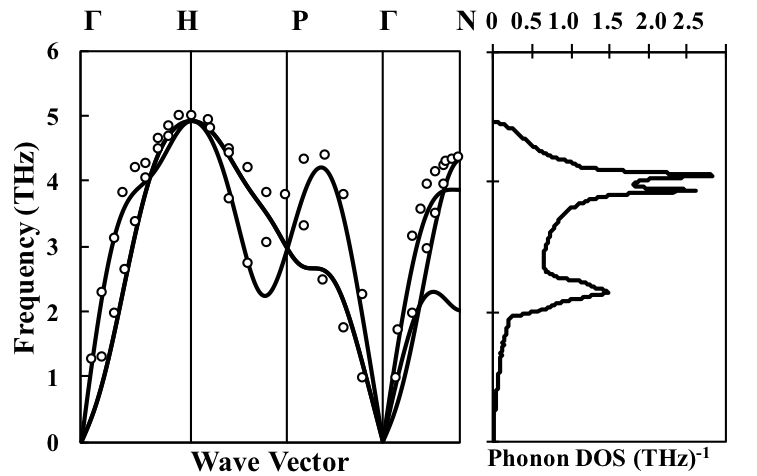
\includegraphics[width=\textwidth]{Chapter-4/Figures/Taphonondos.png}
	\caption{Calculated phonon dispersion curve of bcc-Ta, compared with neutron diffraction experiments ($\circ$) \cite{Taioli2007a} along with the phonon DOS. }
	\label{Ch4-figure:Taphonon}
\end{figure}

\pagebreak
\begin{figure}[H]
	\centering
	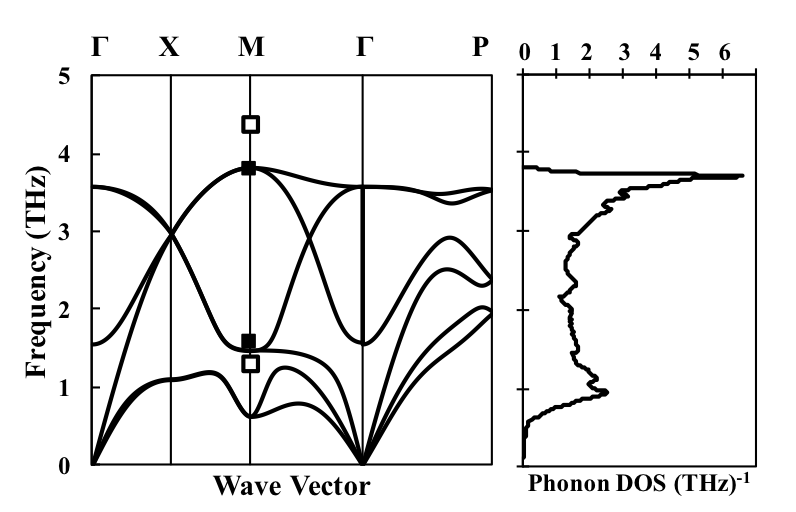
\includegraphics[width=\textwidth]{Chapter-4/Figures/Snphonondos.png}
	\caption{Calculated phonon dispersion curve of bct-Sn on the left and phonon DOS on the right. The open squares ($\square$) are the LO and TO modes from Raman \cite{Olijnyk1992} and the filled squares the theoretical prediction of the LO and TO modes at the M point \cite{Olijnyk1992}.}
	\label{Ch4-figure:Snphonon}
\end{figure}

\pagebreak
\begin{figure}[H]
	\centering
	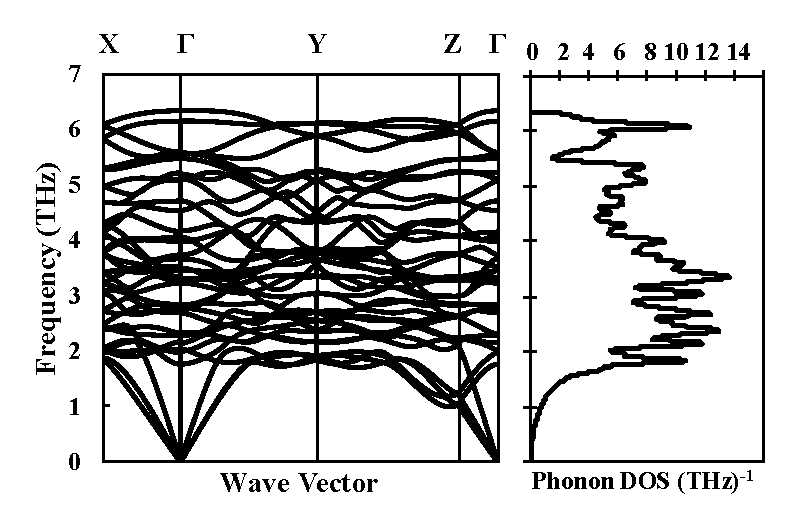
\includegraphics[width=\textwidth]{Chapter-4/Figures/TaSn2phonondos.png}
	\caption{Calculated phonon dispersion curve for TaSn$_2$ at 0 $^\circ$K and the phonon DOS.}
	\label{Ch4-figure:TaSn2phonon}
\end{figure}

\pagebreak
\begin{figure}[H]
	\centering
	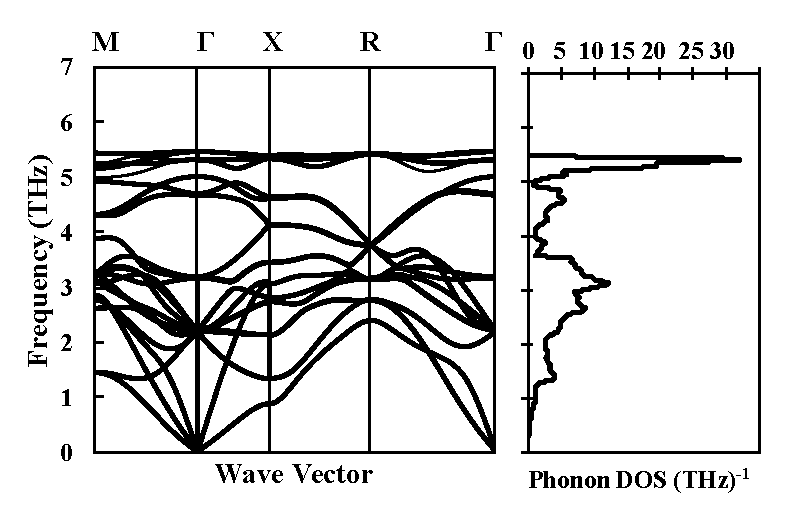
\includegraphics[width=\textwidth]{Chapter-4/Figures/Ta3Snphonondos.png}
	\caption{Calculated phonon dispersion curve of Ta$_3$Sn at 0 $^\circ$K on the left and the phonon DOS on the right.}
	\label{Ch4-figure:Ta3Snphonon}
\end{figure}

\pagebreak
\begin{figure}[H]
	\centering
	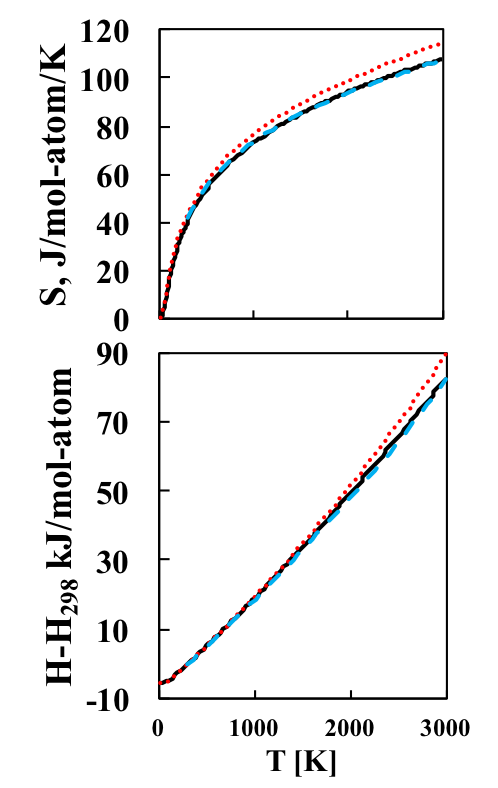
\includegraphics[scale=1.0]{Chapter-4/Figures/Tafinitetemp.png}
	\caption{Comparison of the enthalpy and entropy of bcc-Ta from the Debye model (solid line) and the quasiharmonic phonon calculations (red dotted line) to the SGTE data (blue dashed line) \cite{Dinsdale1991}.}
	\label{Ch4-figure:Tafinitetemp}
\end{figure}

\pagebreak
\begin{figure}[H]
	\centering
	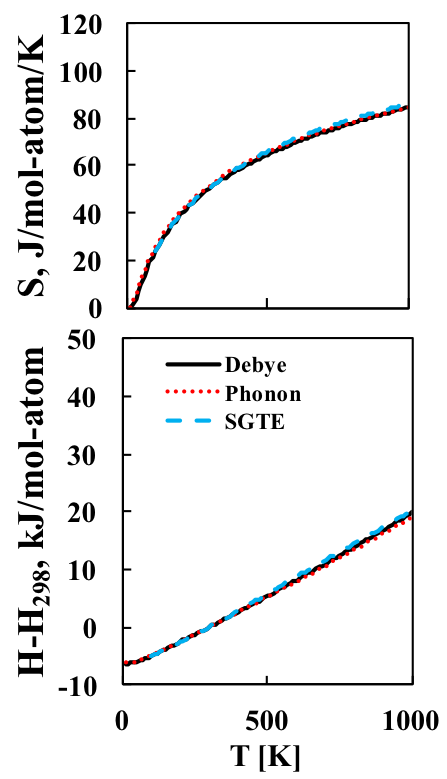
\includegraphics[scale=1.0]{Chapter-4/Figures/Snfinitetemp.png}
	\caption{Comparison of the Gibbs energy of bct-Sn from the Debye model (solid line) and the quasiharmonic phonon calculations (red dotted line) to the SGTE data (blue dashed line) \cite{Dinsdale1991}.}
	\label{Ch4-figure:Snfinitetemp}
\end{figure}

\pagebreak
\begin{figure}[H]
	\centering
	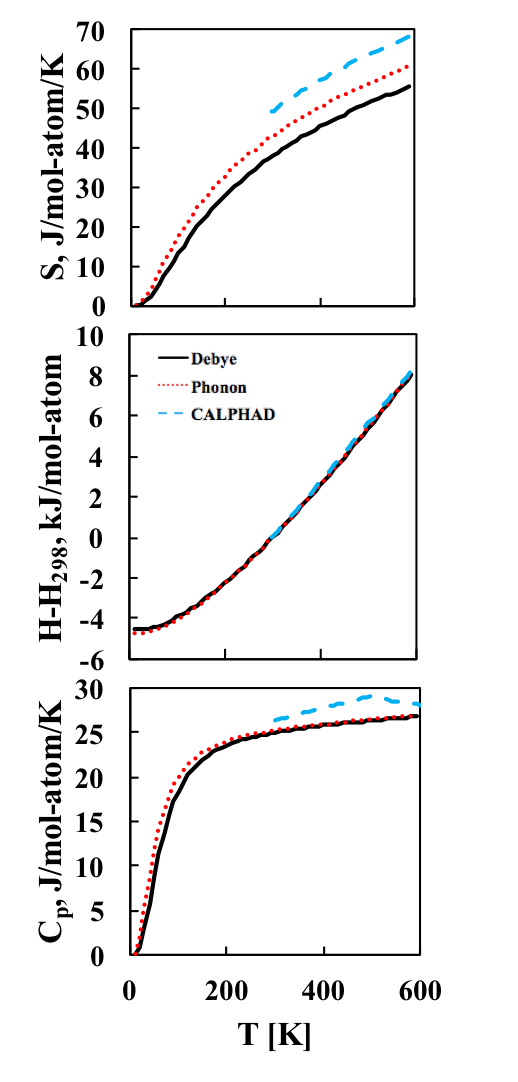
\includegraphics[scale=1.0]{Chapter-4/Figures/TaSn2finitetemp.png}
	\caption{Heat capacity, enthalpy and entropy of TaSn$_2$ using the Debye model (solid line) and the quasiharmonic phonon calculation (red dotted line) from first-principles calculations, compared with those from the current CALPHAD modeling (blue dashed line).}
	\label{Ch4-figure:TaSn2finitetemp}
\end{figure}

\pagebreak
\begin{figure}[H]
	\centering
	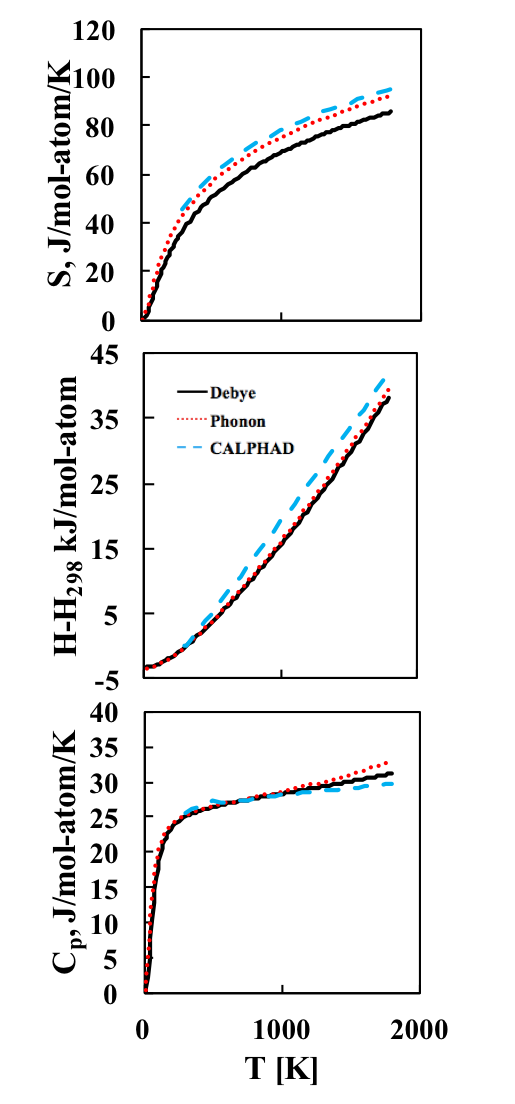
\includegraphics[scale=1.0]{Chapter-4/Figures/Ta3Snfinitetemp.png}
	\caption{Heat capacity, enthalpy and entropy of Ta$_3$Sn using the Debye model (solid line) and the quasiharmonic phonon calculation (red dotted line) compared with those from the current CALPHAD modeling (blue dashed line).}
	\label{Ch4-figure:Ta3Snfinitetemp}
\end{figure}

\pagebreak
\begin{figure}[H]
	\centering
	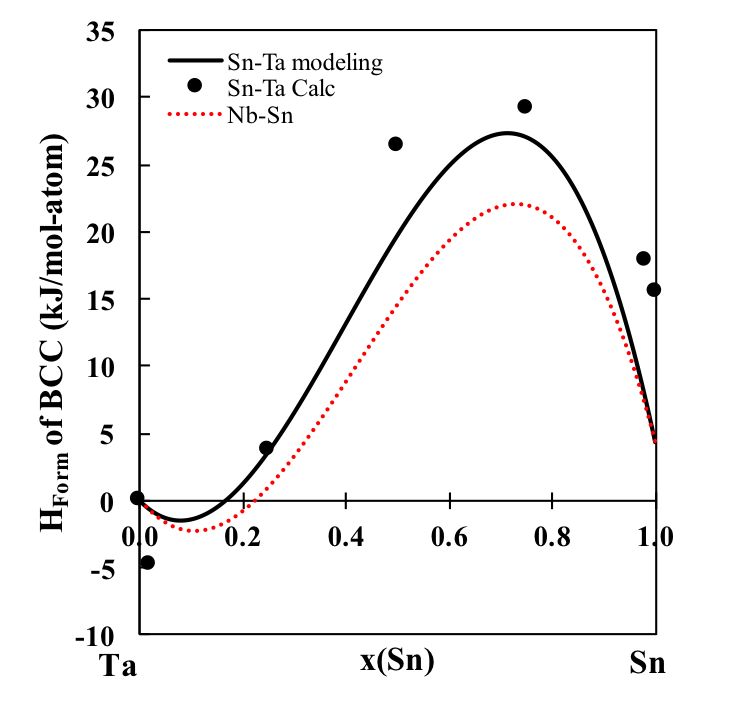
\includegraphics[width=\textwidth]{Chapter-4/Figures/HofForm.png}
	\caption{Heat capacity, enthalpy and entropy of Ta$_3$Sn using the Debye model (solid line) and the quasiharmonic phonon calculation (red dotted line) compared with those from the current CALPHAD modeling (blue dashed line).}
	\label{Ch4-figure:HofForm}
\end{figure}

\pagebreak
\begin{figure}[H]
	\centering
	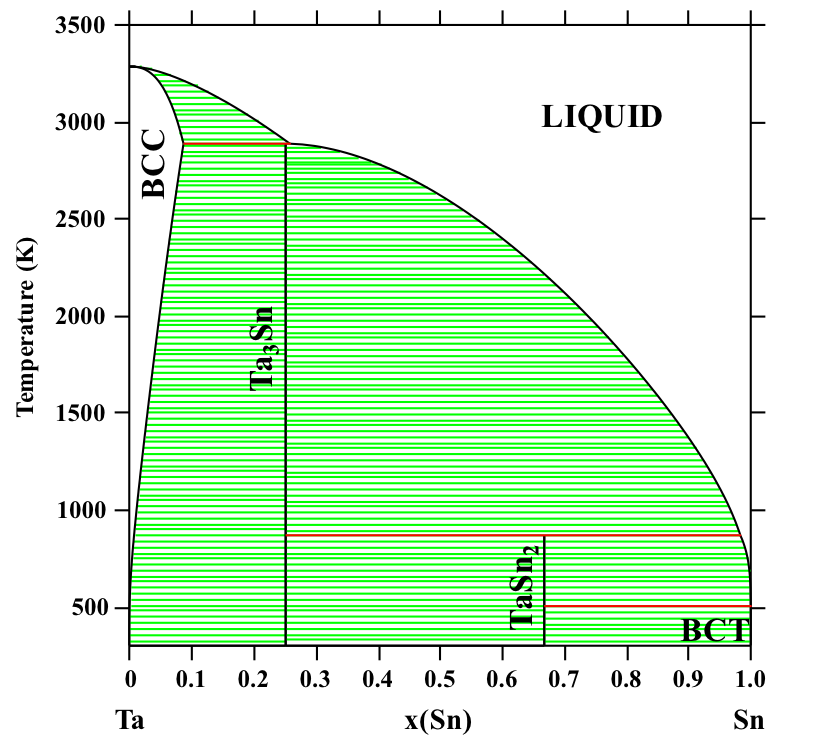
\includegraphics[width=\textwidth]{Chapter-4/Figures/SnTaPD.png}
	\caption{Calculated Sn-Ta phase diagram using the present thermodynamic description.}
	\label{Ch4-figure:SnTaPD}
\end{figure}

\pagebreak
\begin{figure}[H]
	\centering
	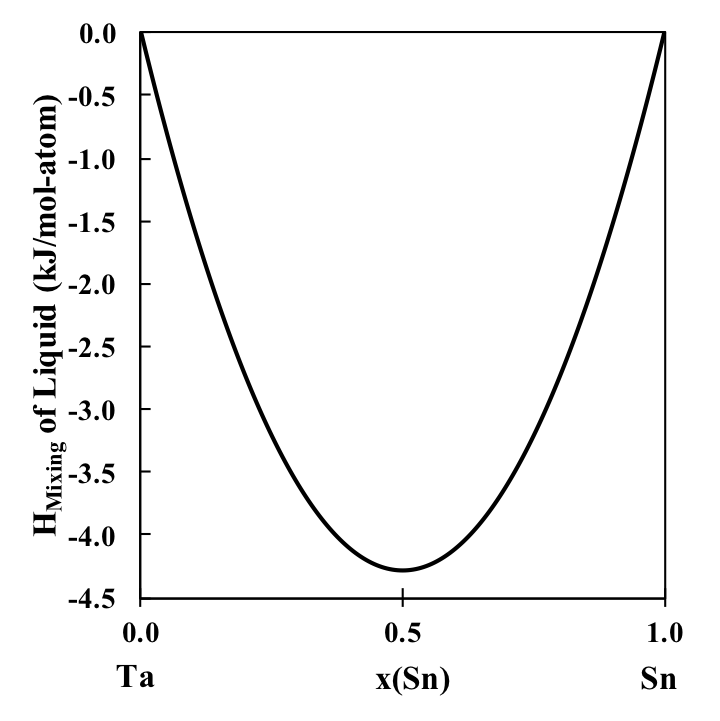
\includegraphics[width=\textwidth]{Chapter-4/Figures/HofMix.png}
	\caption{Enthalpy of mixing of the liquid phase as a function of composition at 298 $^\circ$K and ambient pressure in the Sn-Ta system.}
	\label{Ch4-figure:HofMix}
\end{figure}
\chapter{Effects of alloying elements on the elastic properties of bcc Ti-X alloys}

\section{Introduction}

The present chapter is aimed at studying the effects of alloying elements on the mechanical properties of Ti-alloys as well as completing a database to calculate the elastic properties as a function of composition. This is accomplished by systematically studying the single crystal elastic stiffness coefficients (c$_{ij}$'s) and polycrystalline aggregate properties of bcc Ti-X (X = Mo, Nb, Ta, Sn, Zr) alloys. The elastic properties are calculated using first-principles calculations based on density functional theory (DFT). The composition dependence of the elastic properties of Ti-X alloys is explored through dilute solutions and special quasirandom structures (SQS) \cite{Jiang2004} for concentrated solutions using the methodologies outlined in chapter 2. The obtained elastic properties are then fit using the CALPHAD method and extrapolated to higher order Ti-alloys. 

\section{Modeling and Calculations}

In the present work, the Vienna Ab-initio Simulation Package (VASP) \cite{Kresse1996} was employed to calculate the elastic properties of pure elements and Ti-containing binary systems in the bcc phase. The ion-electron interactions were described using the projector augmented wave (PAW) \cite{Kresse1999,Blochl1994} method. As discussed previously, the use of two X-C functionals were compared in this chapter and based on the results the generalized gradient approximations depicted by Perdew, Burke, and Ernzerhof (PBE-GGA) was employed \cite{Perdew1996a}. For consistency, a 310 eV energy cutoff was adopted for all calculations, which is roughly 1.3 times higher than the default value. The energy convergence criterion of the electronic self-consistency was set as 10$^{-6}$ eV/atom, and the $\Gamma$-centered Monkhorst-Pack scheme was used for Brillouin zone sampling \cite{Kresse1996,Monkhorst1976a}. The k-points grid used for each calculation are listed in appendix C.

For the Ti-X binary systems, calculations for both dilute and SQS solutions were carried out. Three SQS cells with mole fractions of alloying element X atoms at 0.25, 0.5, and 0.75 were employed. Dilute solutions were calculated for each Ti-X binary alloy using different supercell sizes, i.e., Ti-Mo 4 dilute structures (Mo$_{0.98}$Ti$_{0.02}$ 54-atoms, Mo$_{0.94}$Ti$_{0.06}$ 16-atoms, Ti$_{0.88}$Mo$_{0.12}$ 8-atoms, Ti$_{0.94}$Mo$_{0.06}$ 16-atoms), Ti-Nb 4 dilute structures (Nb$_{0.98}$Ti$_{0.02}$ 54-atoms, Nb$_{0.94}$Ti$_{0.06}$ 16-atoms, Ti$_{0.88}$Nb$_{0.12}$ 8-atoms, Ti$_{0.98}$Nb$_{0.02}$ 54-atoms), Ti-Sn 1 dilute structure (Ti$_{0.94}$Sn$_{0.06}$ 16-atoms), Ti-Ta 5 dilute structures (Ta$_{0.98}$Ti$_{0.02}$ 54-atoms, Ta$_{0.94}$Ti$_{0.06}$ 16-atoms, Ti$_{0.88}$Ta$_{0.12}$ 8-atoms, Ti$_{0.94}$Ta$_{0.06}$ 16-atoms, Ti$_{0.98}$Ta$_{0.02}$ 54-atoms), Ti-Zr 2 dilute structures (Zr$_{0.94}$Ti$_{0.06}$ 16-atoms, Ti$_{0.98}$Zr$_{0.02}$ 54-atoms). The interaction parameters for the  elastic stiffness coefficients were then determined according to the methodology laid out in chapter 2.

The first-principles results were then used to model the elastic stiffness coefficients. The modeling was completed by calculating the difference between the first-principles calculations and a linear extrapolation between pure elements. The differences were then used to fit to the interaction parameters. Due to the limitations within the PARROT module, a Mathematica script was used to fit the interaction parameters. The Mathematica script is appended in appendix C. With the focus being Ti-rich alloys, the first-principles results with 70 at. \% Ti or higher were weighted heavier (x6, according to the authors' practices) than the other points for the fittings. The best fit was found by comparing the fittings obtained with one interaction parameter or with two interaction parameters. The moduli values were than calculated from the elastic stiffness coefficients according to the methodology in chapter 2.

\section{Results and discussion}

\subsection{Evaluation of calculation settings}

The X-C functionals of PW91 and PBE were tested on the Ti-Ta binary system. The results are plotted in Figure \ref{Ch5-figure:PBEvsPW91}, showing the $\overline{C}_{44}$ values differing by 10 GPa or less and the $\overline{C}_{11}$ and $\overline{C}_{12}$ values by less than 5 GPa for high Ta contents and by 26 GPa and 13 GPa with 25 at. \% Ta, respectively. Since overall the values vary by an error of less than 0.2 (calculated with Eq. \ref{eq: error}), and the PBE functional was developed as an improvement of the PW91 functional for metals, the PBE functional is chosen for the present work. 

Three magnitudes of strain are tested on the Ti-Mo binary system and plotted in Figure \ref{Ch5-figure:Strain}. The different strain magnitudes do not affect the results significantly. For example, the $\overline{C}_{11}$ values calculated using $\pm$0.01, $\pm$0.013, and $\pm$0.007 strains at Mo$_{0.94}$Ti$_{0.06}$ are 451 GPa, 450 GPa, and 450 GPa, respectively, varying within 1 GPa (< 0.01). The variances in the $\overline{C}_{12}$ and $\overline{C}_{44}$ results are similar. Overall, the variances in the $\overline{C}_{11}$ and $\overline{C}_{12}$ are less than 0.02 (Eq. \ref{eq: error}). The largest variance is in the Ti$_{0.50}$Mo$_{0.50}$ where the $\overline{C}_{44}$ values are 42 GPa, 42 GPa, and 65 GPa calculated with $\pm$0.01, $\pm$0.013, and $\pm$0.007 strains, respectively. Overall, the strain magnitude does not affect the calculated results significantly, and thus the $\pm$0.01 strain magnitude is used for all the calculations.

\subsection{Calculations of elastic coefficients in Ti-X binary systems}

The elastic stiffness coefficients and bulk moduli ($B$) are calculated for the pure elements in the bcc structure and reported in Table \ref{Ch5-table:pureeleelas}. The results in the present work are all obtained at 0 K. The results for Mo, Nb and Ta, which are stable in the bcc structure at low temperatures, are compared with experimental data at temperatures shown in Table \ref{Ch5-table:pureeleelas} \cite{Dickinson1967a,Bolef1961}. The error (Eq. \ref{eq: error}) between the present results and previous results for Mo, Nb and Ta are 0.0261, 0.075, and 0.0425, respectively \cite{Simmons1971b,Dickinson1967a,Bolef1961}. This discrepancy is due to the temperature difference between the experiments and calculations. The calculations are at 0 K while the experimental values were measured at higher temperatures. 

Ti and Zr are stable in the hcp structure at low temperatures, and Sn is stable in the body centered tetragonal and diamond structures at low temperatures. Due to the instability of Ti, Sn and Zr in the bcc structure at low temperatures, their elastic stiffness coefficients are compared to previous first-principles calculations at 0 K \cite{Shang2010b} that used the PW91 functional, and the errors/differences are 0.024, 0.528 and 0.051, respectively. The differences are related to the instability of the bcc structure, the different exchange correlation functionals and the different input parameters chosen. Due to the bcc instability, multiple relaxation schemes are compared in the present work to find the lowest energy structure retaining the bcc symmetry, making the results the most accurate representation of the bcc pure elements.  

Figure \ref{Ch5-figure:tixc11} to Figure \ref{Ch5-figure:tixc44} compare the calculated elastic stiffness coefficients, $\overline{C}_{11}$, $\overline{C}_{12}$, $\overline{C}_{44}$ (circles) with the currently modeled elastic stiffness coefficients (solid line) and linear combination from the pure elements for the Ti-Mo, Ti-Nb, Ti-Sn, Ti-Ta, and Ti-Zr systems. The model parameters are shown in Table \ref{Ch5-table:tixelasip}. The results calculated for the Ti-Mo, Ti-Nb, and Ti-Ta systems are compared with previous calculated results from Ikehata et al. \cite{Ikehata2004}, and the differences are due to the different input parameters and structures used at each composition. Ikehata et al. \cite{Ikehata2004} used the s orbital electrons as the valance electrons for Ti and used the B2 structure for their Ti$_{0.50}$X$_{0.50}$ compositions with Ti at the body centered site and X at the corner sites. For the Ti$_{0.25}$X$_{0.75}$ and Ti$_{0.75}$X$_{0.25}$ structures they used the DO$_{3}$ structure with space group $Fm\overline{3}m$, and not the bcc space group of $Im\overline{3}m$. The present work uses the p electrons as valance electrons for Ti based on updated recommendations by VASP and 16-atom SQS from Jiang et al. \cite{Jiang2004}. The SQS mimic the random substitution of elements with less error and represent the atomic structures of solution phases better than ordered structures. It can be seen that Mo, Nb, and Ta affect the elastic stiffness coefficients in a similar fashion. As shown in Figure \ref{Ch5-figure:tixc11}a, \ref{Ch5-figure:tixc11}b and \ref{Ch5-figure:tixc11}d the $\overline{C}_{11}$ increases in value from Ti to X (X = Mo, Nb, Ta). Figures \ref{Ch5-figure:tixc44}a, \ref{Ch5-figure:tixc44}b and \ref{Ch5-figure:tixc44}d show that the $\overline{C}_{44}$ values first decrease and then increase with the addition of the alloying element X (X = Mo, Nb and Ta). The $\overline{C}_{12}$ values increase by the addition of Mo or Ta (Figure \ref{Ch5-figure:tixc12}a and Figure \ref{Ch5-figure:tixc12}d, respectively), and the $\overline{C}_{12}$ values first decrease and then increase by the addition of Nb (Figure \ref{Ch5-figure:tixc12}b). A similar trend is shown in the $\overline{C}_{11}$ and $\overline{C}_{12}$ data for the Ti-Sn system (Figure \ref{Ch5-figure:tixc11} and Figure \ref{Ch5-figure:tixc12}c). The $\overline{C}_{11}$ and $\overline{C}_{12}$ values first increase and then decrease from pure Ti to pure Sn. As seen in Figure \ref{Ch5-figure:tixc44}c, $\overline{C}_{44}$ first increases in value, then decreases, and then increases again from pure Ti to pure Sn. In the Ti-Zr system, the $\overline{C}_{11}$ and $\overline{C}_{44}$ values first increase and then decrease with increasing Zr concentration (Figure \ref{Ch5-figure:tixc11}e and Figure \ref{Ch5-figure:tixc44}e). For the Ti-Zr system, the $\overline{C}_{12}$ values first decrease and then increase, as shown in Figure \ref{Ch5-figure:tixc12}e. The first-principles calculations based on DFT results for the elastic stiffness coefficients are listed in Table \ref{Ch5-table:tixelassc}.

Figure \ref{Ch5-figure:tixyoungs} summarizes the present Young's moduli results for each Ti-X binary system (circles). The $E$ results for the pure elements and Ti-X binary systems are listed in Table \ref{Ch5-table:tixelasmod}. The lines are the estimated $E$ using the Voigt-Reuss-Hill approach and predicted from the elastic stiffness coefficients that were modeled using Eq. \ref{eq: elastic}. The elastic stiffness coefficients model parameters are shown in Table \ref{Ch5-table:tixelasip}. The average from the Hill approach is plotted as a solid black line while those from the Voigt (high bound) and Reuss (low bound) approaches are plotted as dotted and dashed lines, respectively. For stable structures the Voigt and Reuss approaches do not vary drastically but when the structures are unstable the variance is larger with the average from the Hill approach being the value that the database will predict. The results for the Ti-Mo, Ti-Nb and Ti-Ta systems are compared to available experimental results \cite{Zhang2015,Boyer1994,Sung2015,Ozaki2004,Fedotov1985,Zhou2009a,Zhou2004a} also shown in Figure \ref{Ch5-figure:tixyoungs} and listed in Table \ref{Ch5-table:tixelasmod}. Figure \ref{Ch5-figure:tixyoungs}a compares the present $E$ results for the Ti-Mo alloy system with experimental data from Zhang et al. \cite{Zhang2015}, Collings et al. \cite{Boyer1994} and Sung et al. \cite{Sung2015}. It can be seen that the $E$ increases in value from pure Ti to pure Mo. The results from Sung et al. \cite{Sung2015} differ by about 60 GPa from the present work. However, during the XRD and TEM investigations by Sung et al. \cite{Sung2015}, one of the metastable phases, $\alpha"$ and $\omega$, was observed in the samples in addition to the bcc phase. The formation of the $\alpha"$ and $\omega$ phases causes variations in the elastic properties from those of the single bcc phase. Zhang et al. \cite{Zhang2015} and Collings et al. \cite{Boyer1994} did not observe the formation of either metastable phase. The Young's moduli determined by Zhang et al. \cite{Zhang2015} and Collings et al. \cite{Boyer1994} agree with the present Voigt-Reuss bounds and have an error of 0.39 (Eq. \ref{eq: error}) from the Hill average Young's modulus. 

The present $E$ of the Ti-Nb system are compared with data from Ozaki et al. \cite{Ozaki2004} and Collings et al. \cite{Boyer1994} in Figure \ref{Ch5-figure:tixyoungs}b, showing an increase in $E$ values with an increase in the Nb concentration. The analyses of the samples from the work by Ozaki et al. \cite{Ozaki2004} and Collings et al. \cite{Boyer1994} depict that all alloys contained the single bcc phase. The $E$ from the present first-principles calculations have an error of 0.09 (Eq. \ref{eq: error}) compared to the $E$ determined by Ozaki et al. \cite{Ozaki2004} and Collings et al. \cite{Boyer1994}. 

Figure \ref{Ch5-figure:tixyoungs}d shows the calculated $E$ for the Ti-Ta system in comparison with the experimental values determined by Fedotov et al. \cite{Fedotov1985} and Zhou et al. \cite{Zhou2004a,Zhou2009a}. The $E$ values, in the Ti-Ta system, increase from pure Ti to pure Ta, and the calculated Young's moduli have an error of 0.19 (Eq. \ref{eq: error}) compared to the experimental Young's moduli \cite{Fedotov1985,Zhou2004a,Zhou2009a}.  

The error between the experimentally determined Young's moduli and the calculated Young's moduli is expected due to the temperature difference (calculations at 0 K and experiments at 298 K). The experimentally determined Young's moduli agree well within the Voigt and Reuss bounds, and the present calculations provide good prediction of the elastic properties of the Ti-Mo, Ti-Nb and Ti-Ta alloys as a function of composition.

The calculated Young's moduli for the Ti-Sn (Figure \ref{Ch5-figure:tixyoungs}c) and Ti-Zr (Figure \ref{Ch5-figure:tixyoungs}e) systems cannot be compared to experimental data because the bcc phase is not stable in these systems at low temperatures. For the Ti-Sn alloy system the $E$ values increase from 0 to ~35 at. \% Sn and then decrease from ~35 to 100 at. \% Sn. The $E$, of the Ti-Zr system, increases in value from 0 to 40 at. \% Zr, and then decreases from 40 to 100 at. \% Zr. Figure \ref{Ch5-figure:tixmap} plots the Young's modulus as a function of composition from pure Ti in the bcc structure to the alloying element (X = Mo, Nb, Sn, Ta, Zr) and compares the effects of each alloying element on the Young's modulus. This mapping can be used to find alloy compositions that have the target $E$ values (10-40 GPa). From Figure \ref{Ch5-figure:tixmap}  there are multiple different compositions that have the target $E$.

As discussed in chapter 2, the instability of the bcc phase can be determined by Born's criteria (Eq. \ref{eq: born1}-\ref{eq: born3}). Figure \ref{Ch5-figure:tixc11-c12} shows the $\overline{C}_{11}$-$\overline{C}_{12}$ values from first-principles calculations and the present modeling, indicating the stability and instability regions of the bcc phase in different Ti-alloys. When the $\overline{C}_{11}$ - $\overline{C}_{12}$ is positive the bcc phase is mechanically stable and when the $\overline{C}_{11}$ - $\overline{C}_{12}$ is negative the bcc phase is mechanically unstable. The bcc phase is mechanically unstable at Mo, Nb, Sn, Ta, and Zr concentrations of less than 5.5, 11.5, 51.5, 9.5 and 4.0 at. \%, respectively. Alloying with only 4.0 at. \% Zr stabilizes the bcc phase, which is the lowest alloying concentration of any of the alloying elements even though it is known as a weak $\beta$-stabilizer. 5.5, 9.5 and 11.5 at. \% of Mo, Ta and Nb, respectively, are needed to alloy with Ti in order to stabilize the bcc phase. Mo, Nb, and Ta are similar elements that are all stable in the bcc phase and known to be $\beta$-stabilizers. 51.5 at. \% of Sn is needed to stabilize the bcc phase when alloyed with Ti. Sn is not stable in the bcc phase and is not a $\beta$-stabilizer. Based on the $E$ mapping in Figure \ref{Ch5-figure:tixmap}, the compositions that fall into the target $E$ range for the biomedical application (10-40 GPa) are targeted. However, the bcc phase of the targeted alloy compositions needs to be stable, which is determined by Figure \ref{Ch5-figure:tixc11-c12}. Using these results, the composition range for each Ti-X alloy that has the target $E$ and the bcc phase stable are listed in Table \ref{Ch5-table:targetalloys}. The Ti-Mo, Ti-Nb, Ti-Ta and Ti-Zr alloys show small compositions ranges where both the criteria are met while Ti-Sn has no composition range that stabilizes the bcc phase and has the target $E$. From these results, there are compositions that can be targeted and alloying with more than one element will show other compositions that have the properties desired. 

Figure \ref{Ch5-figure:tixbulk} and Figure \ref{Ch5-figure:tixshear} show the bulk ($B$) and shear ($G$) moduli of the Ti-X (X = Mo, Nb, Sn, Ta, Zr) systems, with the present results (circles), the Hill average (solid black line), and Voigt (purple dashed line) and Reuss (yellow dashed line) bounds plotted. Similar trends in the $B$ and $G$ data are seen for the Ti-Mo, Ti-Nb and Ti-Ta systems. The $B$ and $G$ increase in value with increasing Mo, Nb and Ta concentration, as shown in Figure \ref{Ch5-figure:tixbulk} and Figure \ref{Ch5-figure:tixshear}, respectively. The $B$ and $G$ values increase and then decrease from pure Ti to pure Sn in the Ti-Sn system (Figure 9c and Figure 10c). In the Ti-Zr system, the $B$ decreases in value from pure Ti to pure Zr (Figure \ref{Ch5-figure:tixbulk}e) and the $G$ first increases in value and then decreases from pure Ti to pure Zr (Figure \ref{Ch5-figure:tixshear}e). The predicted $B$ and $G$ values are listed in Table \ref{Ch5-table:tixelasmod}. 

\subsection{Extrapolation to ternary and higher ordered systems}

The interaction parameters in Table \ref{Ch5-table:tixelasip} can be used to predict the elastic stiffness coefficients of higher order Ti-alloys by summing the interaction parameters of each binary alloy contained in the multi-component alloy from Eq. \ref{eq: elastic}. The predicted elastic stiffness coefficients of the multi-component alloys can be used to calculate the Young's modulus as a function of composition. The accuracy of prediction of the elastic properties of higher order Ti alloys are evaluated by comparing the predicted results with previous experimental results \cite{Niinomi2012,Tane2010a,Geetha2009,Mohammed2014} as shown in Figure \ref{Ch5-figure:tixdatabase} and Table \ref{Ch5-table:tixdatacomp}. The black diagonal line represents a perfect correlation between the predicted and experimental Young's moduli. The grey region indicates the error (3 GPa) in the first-principles calculations, which is the average variance in $\overline{C}_{11}$, $\overline{C}_{12}$ and $\overline{C}_{44}$ from Eq. \ref{eq: averagec11}-\ref{eq: averagec44}. 

It can be seen that the difference between experimental Young's moduli at the same composition from Niinomi et al. \cite{Niinomi2012}, Geetha et al. \cite{Geetha2009}, Tane et al. \cite{Tane2010a} and Mohammad et al. \cite{Mohammed2014} varies from 2 GPa to 46 GPa with different heat treatments and measuring techniques. The scattering in the Young's moduli among experimental measurements is denoted by the vertical error bars in Figure \ref{Ch5-figure:tixdatabase}. The horizontal error bars show the Young's moduli ranges from the Reuss and Voigt bounds with the average from the Hill approach marked by the circle. The experimental Young's moduli deviate from the present predictions by 0.69 to 14 GPa. This difference can be contributed to the temperature difference between the first-principles data and the experimental results and uncertainties in calculations and experiments. Considering the fact that the experimental results from the literature at the same composition vary drastically, the present first-principles calculations give a good representation of the elastic properties of higher order Ti-alloys. It is hypothesized that introducing the binary interaction parameters of non-Ti containing alloys in the system and the ternary interaction parameters can further improve the database predictions. 

\section{Conclusion}

The elastic properties of five bcc Ti-X (X = Mo, Nb, Sn, Ta, Zr) systems, including the elastic stiffness coefficients, bulk modulus, shear modulus, and Young's modulus, were systematically studied using first-principles calculations at different compositions. The CALPAHD methodology was used to evaluate interaction parameters for the Ti-X elastic stiffness coefficients as a function of composition and the polycrystalline aggregate properties were predicted using the Voigt-Reuss-Hill approach. The present calculations showed that 5.5, 11.5, 51.5, 9.5, and 4.0 at. \% of Mo, Nb, Sn, Ta and Zr, respectively, are required to stabilize the bcc structure according to the Born criteria. The trends observed were summarized for each Ti-X (X= Mo, Nb, Sn, Ta, Zr) binary system. Alloying with Mo, Nb, and Ta resulted in similar trends, which is probably because Mo, Nb, and Ta are strong bcc stabilizers and stable in the bcc structure at room temperature. The interaction parameters determined in the current work were used to predict the elastic properties of higher order alloys. The accuracy of the databases predictions of the Young's modulus was evaluated by comparing the calculated and experimental Young's moduli. Overall, the database predicted the $E$ values on average within 7 GPa and provided good predictions of the elastic properties of Ti-alloys in the bcc phase as a function of composition. 

\newpage
\begin{table}[H]
	\caption{Calculated pure element elastic stiffness coefficients and the bulk modulus $B$ (in GPa) by X-C functional of PBE are compared with the previous first-principles calculations (FP) by X-C functional PW91 and experiments (Expt). Sv, pv and d referring to the s, p, and d states being treated as valance, respectively.}
	\centering
	\begin{tabular}{ c c c c c c }
		\hline
		Pure Elements & & $\bar{C}_{11}$ & $\bar{C}_{11}$  & $\bar{C}_{11}$ & \textit{B}\\
		\hline
		Ti$\_$sv & This work 0 K & 93 & 115 & 41 & 108\\
		& Calc 0 K \cite{Shang2010b} & 96 & 116 & 40 & 107\\
		Mo$\_$pv & This work 0 K & 475 & 164 & 108 & 268\\
		& Expt 73 K \cite{Simmons1971b} & 473 & 156 & 111 &\\
		& Expt 300 K \cite{Dickinson1967a} & 473 & 160 & 109 & 261\\
		Nb$\_$sv & This work 0 K & 245 & 144 & 27 & 178\\
		& Expt 4 K \cite{Simmons1971b} & 253 & 133 & 31 & \\
		& Expt 300 K \cite{Bolef1961} & 247 & 135 & 29 & 172\\
		Sn$\_$d & This work 0 K & 50 & 52 & 29 & 51\\
		& Calc 0 K \cite{Shang2010b} & 30 & 60 & 18 & 48\\
		Ta$\_$pv & This work 0 K & 278 & 164 & 81 & 202\\
		& Expt 0 K \cite{Simmons1971b} & 266 & 158 & 87 & \\
		& Expt 300 K \cite{Bolef1961} & 267 & 161 & 83 & 196\\
		Zr$\_$sv & This work 0 K & 86 & 91 & 32 & 89\\
		& Calc 0 K \cite{Shang2010b} & 82 & 94 & 30 & 90\\
		\hline
	\end{tabular}
	\label{Ch5-table:pureeleelas}
\end{table}
\clearpage
%%%

\newpage
\begin{table}[H]
	\caption{Evaluated interaction parameters $L_0$ and $L_1$ using the R-K polynomial Eq. \ref{eq: elastic} for the elastic stiffness coefficients for the Ti-X binary systems.}
	\centering
	\begin{tabular}{ c c c c c c c }
		\hline
		Alloy & Interaction Parameter & Ti-Mo & Ti-Nb & Ti-Sn & Ti-Ta & Ti-Zr\\
		\hline
		$\bar{C}_{11}$ & $L_0$ & -22.16 & 40.46 & 119.46 & 83.65 & 246.97\\
		& $L_1$ & 0 & 0 & 0 & -67.76 & -135.95\\
		$\bar{C}_{12}$ & $L_0$ & -36.40 & -32.39 & 15.90 & 38.05 & -110.53\\
		& $L_1$ & 0 & 0 & -146.80 & 0 & 78.00\\
		$\bar{C}_{44}$ & $L_0$ & -142.9 & -41.54 & 59.79 & -51.96 & 70.06\\
		& $L_1$ & 0 & -41.95 & -94.38 & 0 & 0\\	
		\hline
	\end{tabular}
	\label{Ch5-table:tixelasip}
\end{table}
\clearpage
%%%

\newpage
\begin{longtable}[H]{ c c c c c}
	\caption{First-principles calculations of the elastic stiffness coefficients $\overline{C}_{11}$, $\overline{C}_{12}$, and $\overline{C}_{44}$ for different atomic percent compositions of the bcc Ti-X binary systems at 0 K.}	\label{Ch5-table:tixelassc} \\
	\hline
	Reference & Ti$_{1-b}$X$_b$ & $\overline{C}_{11}$ & $\overline{C}_{12}$ & $\overline{C}_{44}$\\
	\hline
	\endhead
	\hline
	\endfoot
	This work & Ti & 93 & 115 & 41\\
	This work & Ti$_{0.94}$Mo$_{0.06}$ & 124 & 111 & 38\\
	This work & Ti$_{0.87}$Mo$_{0.13}$ & 146 & 113 & 29\\
	This work & Ti$_{0.75}$Mo$_{0.25}$ & 178 $\pm$3 & 123 $\pm$15 & 32 $\pm$11\\
	This work & Ti$_{0.50}$Mo$_{0.50}$ & 268 $\pm$9 & 136 $\pm$19 & 42 $\pm$9\\
	This work & Ti$_{0.25}$Mo$_{0.75}$ & 385 $\pm$9 & 146 $\pm$6 & 66 $\pm$6\\
	This work & Ti$_{0.06}$Mo$_{0.94}$ & 451 & 158 & 96\\
	This work & Ti$_{0.02}$Mo$_{0.98}$ & 464 & 163 & 100\\
	This work & Mo & 475 & 164 & 108\\
	This work & Ti$_{0.98}$Nb$_{0.02}$ & 93 & 115 & 35\\
	This work & Ti$_{0.87}$Nb$_{0.13}$ & 116 & 116 & 37\\
	This work & Ti$_{0.75}$Nb$_{0.25}$ & 140 $\pm$11 & 116 $\pm$13 & 34 $\pm$10\\
	This work & Ti$_{0.50}$Nb$_{0.50}$ & 181 $\pm$9 & 121 $\pm$2 & 31 $\pm$10\\
	This work & Ti$_{0.25}$Nb$_{0.75}$ & 208 $\pm$3 & 130 $\pm$4 & 15 $\pm$10\\
	This work & Ti$_{0.06}$Nb$_{0.94}$ & 242 & 134 & 18\\
	This work & Ti$_{0.02}$Nb$_{0.98}$ & 242 & 134 & 18\\
	This work & Nb & 245 & 144 & 27\\
	This work & Ti$_{0.94}$Sn$_{0.06}$ & 100 & 122 & 46 \\
	This work & Ti$_{0.75}$Sn$_{0.25}$ & 105 $\pm$5 & 114 $\pm$2 & 60 $\pm$4\\
	This work & Ti$_{0.50}$Sn$_{0.50}$ & 88 $\pm$9 & 93 $\pm$9 & 46 $\pm$4\\
	This work & Ti$_{0.25}$Sn$_{0.75}$ & 92 $\pm$9 & 55 $\pm$7 & 35 $\pm$8\\
	This work & Sn & 50 & 52 & 29\\
	This work & Ti$_{0.98}$Ta$_{0.02}$ & 100 & 115 & 39 \\
	This work & Ti$_{0.94}$Ta$_{0.06}$ & 116 & 113 & 30 \\
	This work & Ti$_{0.87}$Ta$_{0.13}$ & 120 & 121 & 39 \\
	This work & Ti$_{0.75}$Ta$_{0.25}$ & 167 $\pm$1 & 140 $\pm$3 & 45\\
	This work & Ti$_{0.50}$Ta$_{0.50}$ & 208 $\pm$1 & 159 & 51 $\pm$3\\
	This work & Ti$_{0.25}$Ta$_{0.75}$ & 239 $\pm$7 & 143 $\pm$5 & 62 $\pm$3\\
	This work & Ti$_{0.06}$Ta$_{0.94}$ & 257 & 158 & 72\\
	This work & Ti$_{0.02}$Ta$_{0.98}$ & 264 & 163 & 72\\
	This work & Ta & 278 & 164 & 81\\
	This work & Ti$_{0.98}$Zr$_{0.02}$ & 112 & 106 & 43\\
	This work & Ti$_{0.75}$Zr$_{0.25}$ & 148 $\pm$14 & 82 $\pm$7 & 54 $\pm$7\\
	This work & Ti$_{0.50}$Zr$_{0.50}$ & 152 $\pm$17 & 76 $\pm$12 & 48 $\pm$12\\
	This work & Ti$_{0.25}$Zr$_{0.75}$ & 126 $\pm$12 & 82 $\pm$3 & 45 $\pm$3\\
	This work & Ti$_{0.06}$Zr$_{0.94}$ & 89 & 90 & 34\\
	This work & Zr & 86 & 91 & 32\\
\end{longtable}
%%%

\newpage
\begin{longtable}[H]{ c c c c c}
	\caption{First-principles calculations of the bulk modulus $B$, shear modulus $G$, and Young's modulus $E$ in GPa for different atomic percent compositions of the bcc Ti-X binary systems at 0 K. As well as experimental data for the Young's modulus obtained at 300 K by the reference stated.} 	\label{Ch5-table:tixelasmod} \\
	\hline
	Reference & Ti$_{1-b}$X$_b$ & \textit{B} & \textit{G} & \textit{E}\\
	\hline
	\endhead
	\hline
	\endfoot
	This work & Ti & 108 & -12.91 & -40.34\\
	This work & Ti$_{0.94}$Mo$_{0.06}$ & 115 & 20 & 54\\
	This work & Ti$_{0.87}$Mo$_{0.13}$ & 124 & 23 & 65\\
	This work & Ti$_{0.75}$Mo$_{0.25}$ & 141 $\pm$15 & 30 $\pm$15 & 84 $\pm$15\\
	This work & Ti$_{0.50}$Mo$_{0.50}$ & 180 $\pm$19 & 51 $\pm$19 & 138 $\pm$19\\
	This work & Ti$_{0.25}$Mo$_{0.75}$ & 226 $\pm$9 & 84 $\pm$9 & 224 $\pm$9\\
	This work & Ti$_{0.06}$Mo$_{0.94}$ & 256 & 114 & 397\\
	This work & Ti$_{0.02}$Mo$_{0.98}$ & 263 & 118 & 308\\
	This work & Mo & 268 & 125 & 325\\
	Expt 300 K \cite{Zhang2015} & Ti$_{0.92}$Mo$_{0.08}$ & & & 83\\
	Expt 300 K \cite{Zhang2015} & Ti$_{0.88}$Mo$_{0.12}$ & & & 90\\
	Expt 300 K \cite{Boyer1994} & Ti$_{0.92}$Mo$_{0.08}$ & & & 84\\
	Expt 300 K \cite{Boyer1994} & Ti$_{0.89}$Mo$_{0.11}$ & & & 89\\
	Expt 300 K \cite{Boyer1994} & Ti$_{0.82}$Mo$_{0.18}$ & & & 101\\
	This work & Ti$_{0.98}$Nb$_{0.02}$ & 108 & -18 & -56\\
	This work & Ti$_{0.87}$Nb$_{0.13}$ & 116 & 11 & 31\\
	This work & Ti$_{0.75}$Nb$_{0.25}$ & 124 $\pm$13 & 22 $\pm$13 & 63 $\pm$13\\
	This work & Ti$_{0.50}$Nb$_{0.50}$ & 141 $\pm$9 & 31 $\pm$10 & 86 $\pm$10\\
	This work & Ti$_{0.25}$Nb$_{0.75}$ & 156 $\pm$4 & 22 $\pm$10 & 64 $\pm$10\\
	This work & Ti$_{0.06}$Nb$_{0.94}$ & 170 & 28 & 81\\
	This work & Ti$_{0.02}$Nb$_{0.98}$ & 170 & 28 & 81\\
	This work & Nb & 178 & 35 & 98\\
	Expt 300 K \cite{Ozaki2004} & Ti$_{0.71}$Nb$_{0.29}$ & & & 67\\
	Expt 300 K \cite{Ozaki2004} & Ti$_{0.66}$Nb$_{0.34}$ & & & 74\\
	Expt 300 K \cite{Ozaki2004} & Ti$_{0.56}$Nb$_{0.44}$ & & & 84\\
	Expt 300 K \cite{Boyer1994} & Ti$_{0.74}$Nb$_{0.26}$ & & & 64\\
	Expt 300 K \cite{Boyer1994} & Ti$_{0.70}$Nb$_{0.30}$ & & & 65\\
	Expt 300 K \cite{Boyer1994} & Ti$_{0.66}$Nb$_{0.34}$ & & & 73\\
	Expt 300 K \cite{Boyer1994} & Ti$_{0.56}$Nb$_{0.44}$ & & & 83\\
	This work & Ti$_{0.94}$Sn$_{0.06}$ & 115 & -10 & -30\\
	This work & Ti$_{0.75}$Sn$_{0.25}$ & 111 $\pm$5 & 11 $\pm$5 & 31 $\pm$5\\
	This work & Ti$_{0.50}$Sn$_{0.50}$ & 91 $\pm$9 & 10 $\pm$9 & 29 $\pm$9\\
	This work & Ti$_{0.25}$Sn$_{0.75}$ & 67 $\pm$9 & 27 $\pm$9 & 72 $\pm$9\\
	This work & Sn & 51 & 7 & 21\\
	This work & Ti$_{0.98}$Ta$_{0.02}$ & 110 & -3 & -9\\
	This work & Ti$_{0.94}$Ta$_{0.06}$ & 114 & 11 & 32\\
	This work & Ti$_{0.87}$Ta$_{0.13}$ & 121 & 11 & 32\\
	This work & Ti$_{0.75}$Ta$_{0.25}$ & 149 $\pm$3 & 28 $\pm$3 & 78 $\pm$3\\
	This work & Ti$_{0.50}$Ta$_{0.50}$ & 175 $\pm$1 & 38 $\pm$3 & 106 $\pm$3\\
	This work & Ti$_{0.25}$Ta$_{0.75}$ & 175 $\pm$7 & 56 $\pm$7 & 152 $\pm$7\\
	This work & Ti$_{0.06}$Ta$_{0.94}$ & 191 & 62 & 168\\
	This work & Ti$_{0.02}$Ta$_{0.98}$ & 197 & 62 & 169\\
	This work & Ta & 202 & 70 & 189\\
	Expt 300 K \cite{Fedotov1985} & Ti$_{0.62}$Ta$_{0.38}$ & & & 62\\
	Expt 300 K \cite{Fedotov1985} & Ti$_{0.58}$Ta$_{0.42}$ & & & 79\\
	Expt 300 K \cite{Fedotov1985} & Ti$_{0.52}$Ta$_{0.48}$ & & & 95\\
	Expt 300 K \cite{Zhou2004a} & Ti$_{0.62}$Ta$_{0.38}$ & & & 67\\
	Expt 300 K \cite{Zhou2004a} & Ti$_{0.49}$Ta$_{0.51}$ & & & 105\\
	This work & Ti$_{0.98}$Zr$_{0.02}$ & 108 & 17 & 48\\
	This work & Ti$_{0.75}$Zr$_{0.25}$ & 104 $\pm$14 & 44 $\pm$14 & 116 $\pm$14\\
	This work & Ti$_{0.50}$Zr$_{0.50}$ & 101 $\pm$17 & 44 $\pm$17 & 115 $\pm$17\\
	This work & Ti$_{0.25}$Zr$_{0.75}$ & 97 $\pm$12 & 34 $\pm$12 & 91 $\pm$12\\
	This work & Ti$_{0.06}$Zr$_{0.94}$ & 90 & 9 & 27\\
	This work & Zr & 89 & 6 & 16\\
\end{longtable}
%%%

\newpage
\begin{table}[H]
	\caption{Compositions of the binary alloys that fall in the target $E$ range compared to the bcc phase stability can predict the alloy compositions where the $E$ is close to bone and the bcc phase is stable and those compositions can be targeted.}
	\centering
	\begin{tabular}{ c c c c }
		\hline
		Alloy & at Target $E$ & bcc stabilized & Target Compositions\\
		\hline
		Ti-Mo & Pure Ti to 0.10 mol Mo & > 0.055 mol Mo & 0.055 to 0.10 mol Mo\\
		Ti-Nb & Pure Ti to 0.20 mol Nb & > 0.115 mol Nb & 0.115 to 0.20 mol Nb\\		
		Ti-Sn & Pure Ti to 0.40 mol Sn & > 0.515 mol Sn & N/A\\		
		Ti-Ta & Pure Ti to 0.15 mol Ta & > 0.095 mol Ta & 0.095 to 0.15 mol Ta\\
		Ti-Zr & Pure Ti to 0.05 mol Zr & > 0.040 mol Zr & 0.040 to 0.05 mol Zr\\		
		\hline
	\end{tabular}
	\label{Ch5-table:targetalloys}
\end{table}
\clearpage
%%%

\newpage
\begin{table}[H]
	\caption{Predicted Young's moduli (in GPa) of higher order alloys in the bcc phase compared to experimental values found with both the weight percent and atomic percent listed.}
	\centering
	\begin{tabular}{ c c c c }
		\hline
		Alloy Name (wt. \%) & at. \% & Calc $E$ & Expt $E$\\
		\hline
		Ti-35Nb-7Zr-5Ta \cite{Geetha2009} & Ti-24Nb-5Zr-2Ta & 81 & 80\\
		Ti-29Nb-13Ta-4.6Zr \cite{Geetha2009}  & Ti-20Nb-5Ta-3Zr & 76 & 75\\
		Ti-29Nb-13Ta-6Sn \cite{Geetha2009} & Ti-21Nb-5Ta-3Sn & 68 & 74\\
		Ti-29Nb-13Ta-4.6Sn \cite{Geetha2009} & Ti-20Nb-5Ta-3Sn & 67 & 66\\
		Ti-29Nb-13Ta-4.5Zr \cite{Geetha2009} & Ti-20Nb-5Ta-3Zr & 76 & 65\\
		Ti-29Nb-13Ta-4.6Zr \cite{Tane2010a} & Ti-21Nb-5Ta-3Zr & 76 & 64\\
		Ti-30Nb-10Ta-5Zr \cite{Tane2010a} & Ti-23Nb-4Ta-3Zr & 77 & 64\\
		Ti-35Nb-10Ta-5Zr \cite{Tane2010a} & Ti-25Nb-4Ta-4Zr & 80 & 65\\
		Ti-24Nb-4Zr-7.9Sn \cite{Mohammed2014} & Ti-15Nb-3Zr-4Sn & 65 & 54\\
		Ti-35Nb-2Ta-3Zr \cite{Mohammed2014} & Ti-23Nb-1Ta-2Zr & 69 & 61\\
		Ti-29Nb-11Ta-5Zr \cite{Mohammed2014} & Ti-20Nb-6Ta-2Zr & 74 & 60\\
		Ti-10Zr-5Ta-5Nb \cite{Mohammed2014} & Ti-6Zr-1Ta-3Nb & 64 & 52\\
		Ti-29Nb-13Ta-2Sn \cite{Mohammed2014} & Ti-20Nb-5Ta-1Sn & 66 & 62\\
		\hline
	\end{tabular}
	\label{Ch5-table:tixdatacomp}
\end{table}
\clearpage
%%%

\pagebreak
\begin{figure}[H]
	\centering
	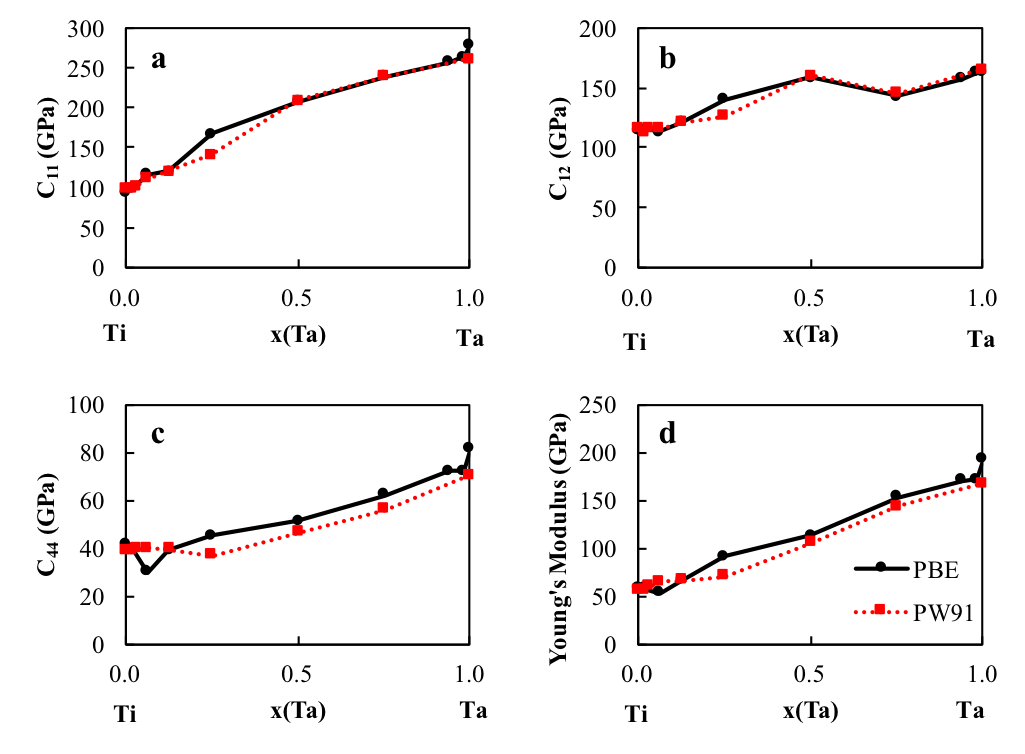
\includegraphics[width=\textwidth]{Chapter-5/Figures/PBEvsPW91.png}
	\caption{Elastic stiffness coefficients of the bcc Ti-Ta binary system calculated with the PW91 and PBE exchange correction functions, respectively.}
	\label{Ch5-figure:PBEvsPW91}
\end{figure}

\pagebreak
\begin{figure}[H]
	\centering
	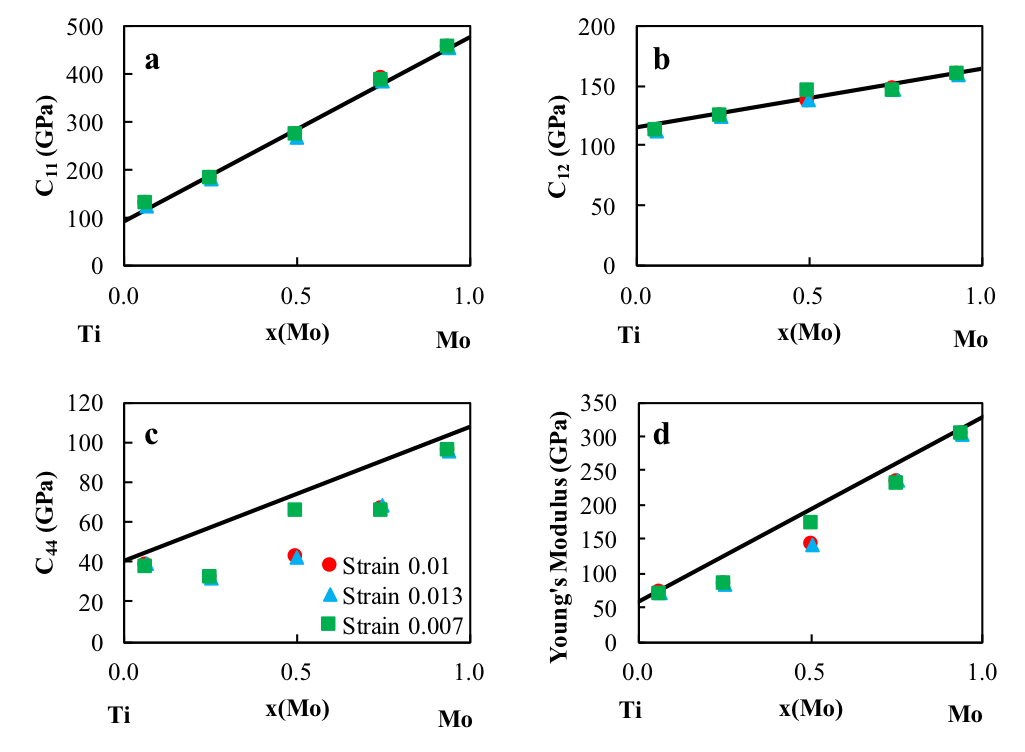
\includegraphics[width=\textwidth]{Chapter-5/Figures/Strain.png}
	\caption{Elastic stiffness coefficients for the bcc Ti-Mo binary system calculated with strains, $\pm$0.01, $\pm$0.013 and $\pm$0.07, respectively, showing comparable results.}
	\label{Ch5-figure:Strain}
\end{figure}

\pagebreak
\begin{figure}[H]
	\centering
	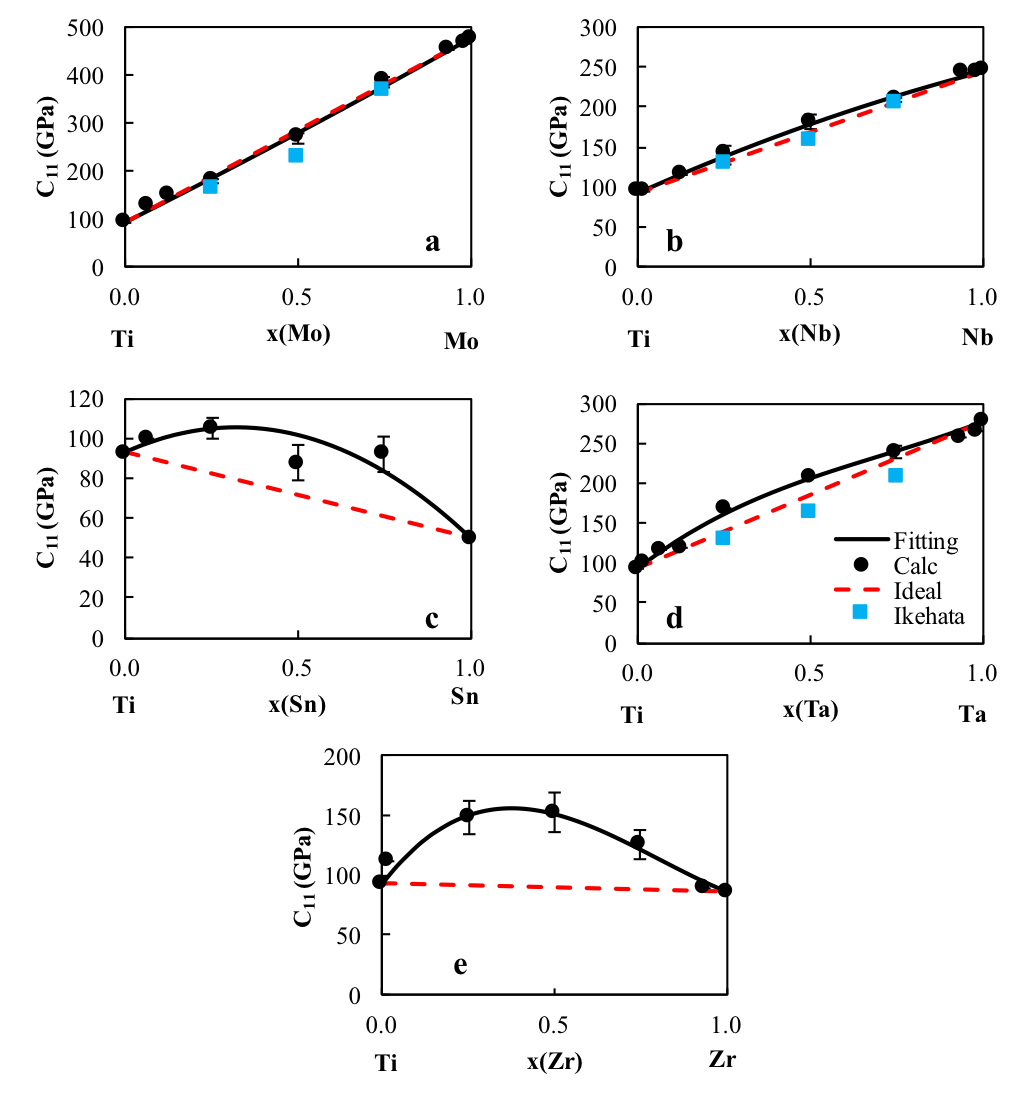
\includegraphics[width=\textwidth]{Chapter-5/Figures/tixc11.png}
	\caption{Calculated $\overline{C}_{11}$ values (circles) plotted with their errors as well as the linear combination of the pure element (red dashed line) and the present modeling (black dashed line) for five Ti-X binary systems (X = Mo, Nb, Ta, Sn, Zr). Ti-Mo, Ti-Nb, and Ti-Ta alloys are compared with previous calculations from Ikehata et al. \cite{Ikehata2004}.}
	\label{Ch5-figure:tixc11}
\end{figure}

\pagebreak
\begin{figure}[H]
	\centering
	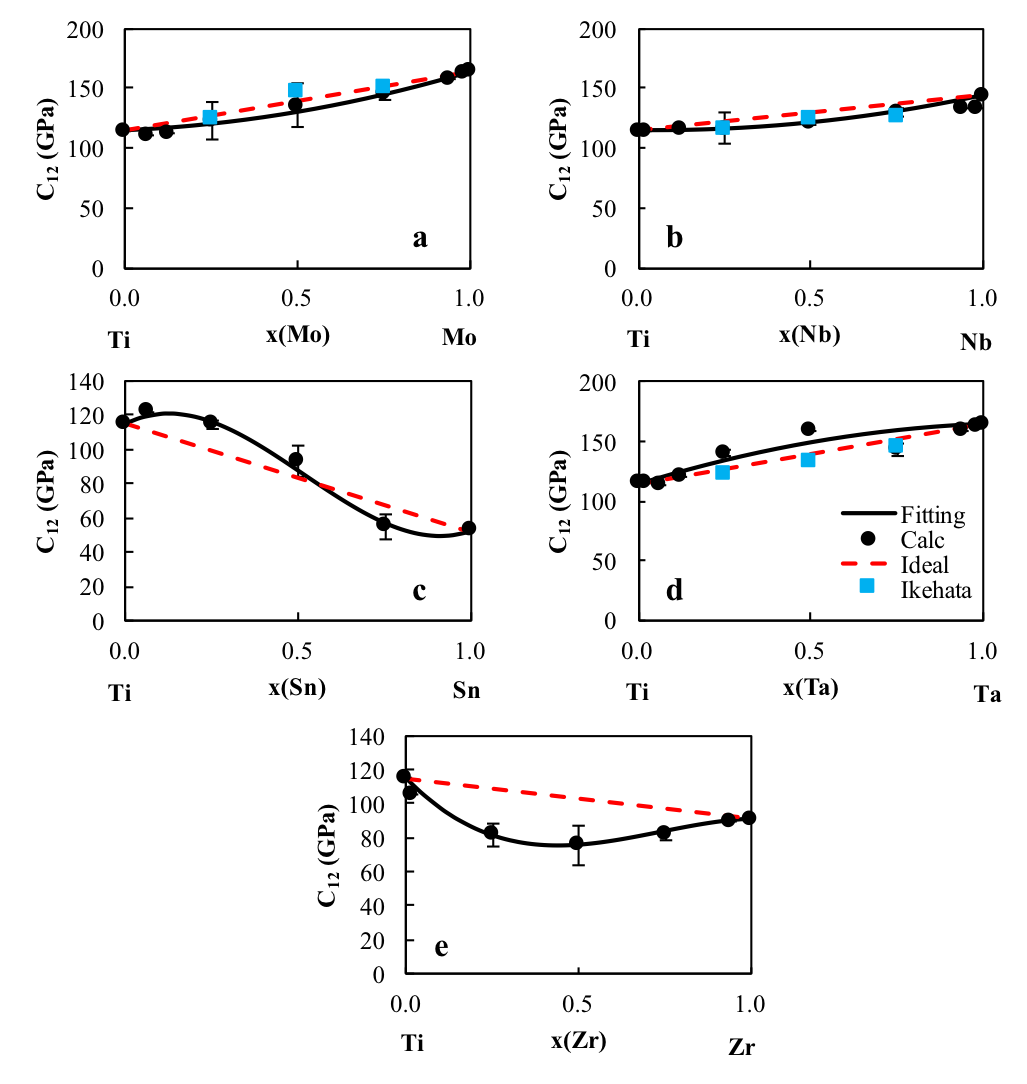
\includegraphics[width=\textwidth]{Chapter-5/Figures/tixc12.png}
	\caption{Calculated $\overline{C}_{12}$ values (circles) plotted with their errors as well as the linear combination of the pure element (red dashed line) and the present modeling (black dashed line) for five Ti-X binary systems (X = Mo, Nb, Ta, Sn, Zr). Ti-Mo, Ti-Nb, and Ti-Ta alloys are compared with previous calculations from Ikehata et al. \cite{Ikehata2004}.}
	\label{Ch5-figure:tixc12}
\end{figure}

\pagebreak
\begin{figure}[H]
	\centering
	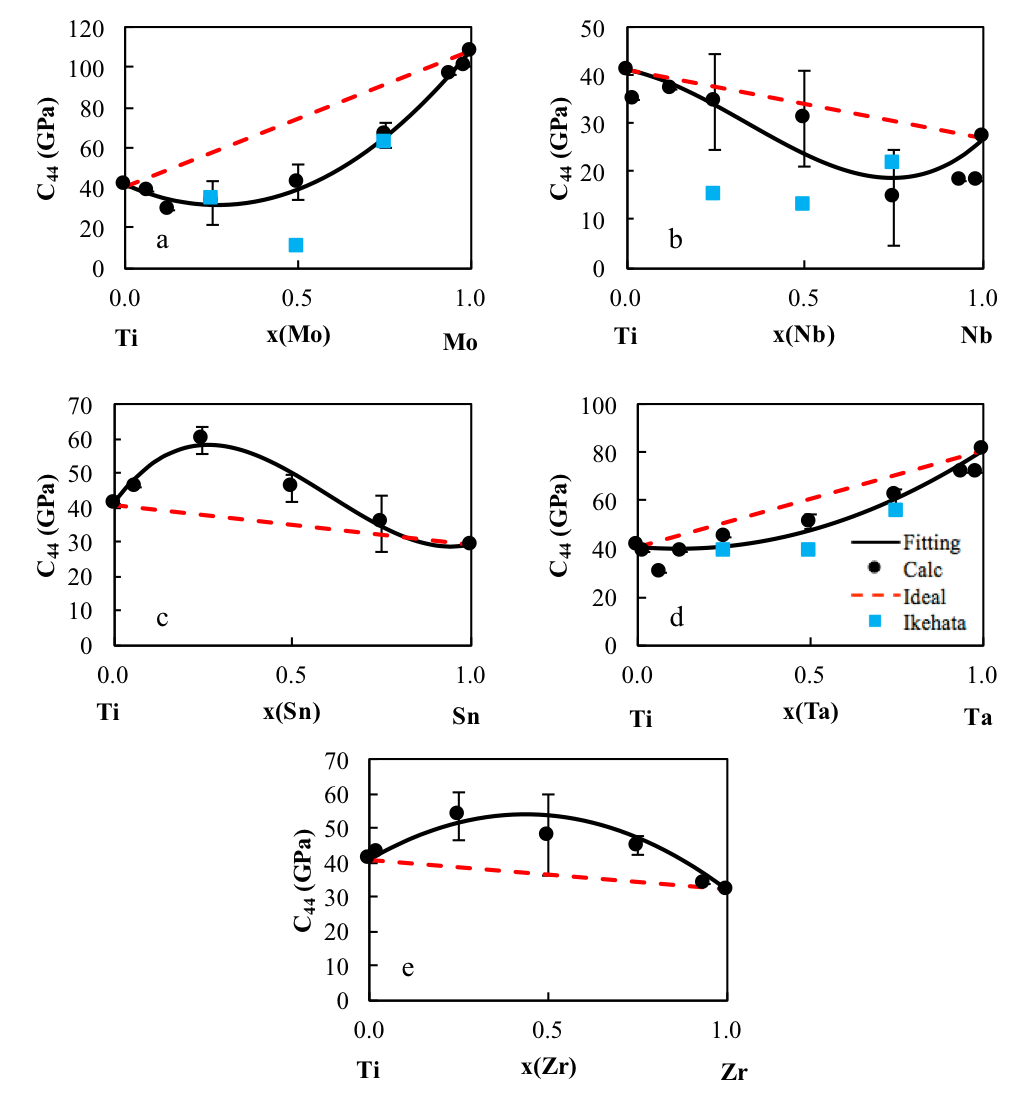
\includegraphics[width=\textwidth]{Chapter-5/Figures/tixc44.png}
	\caption{Calculated $\overline{C}_{44}$ values (circles) plotted with their errors as well as the linear combination of the pure element (red dashed line) and the present modeling (black dashed line) for five Ti-X binary systems (X = Mo, Nb, Ta, Sn, Zr). Ti-Mo, Ti-Nb, and Ti-Ta alloys are compared with previous calculations from Ikehata et al. \cite{Ikehata2004}.}
	\label{Ch5-figure:tixc44}
\end{figure}

\pagebreak
\begin{figure}[H]
	\centering
	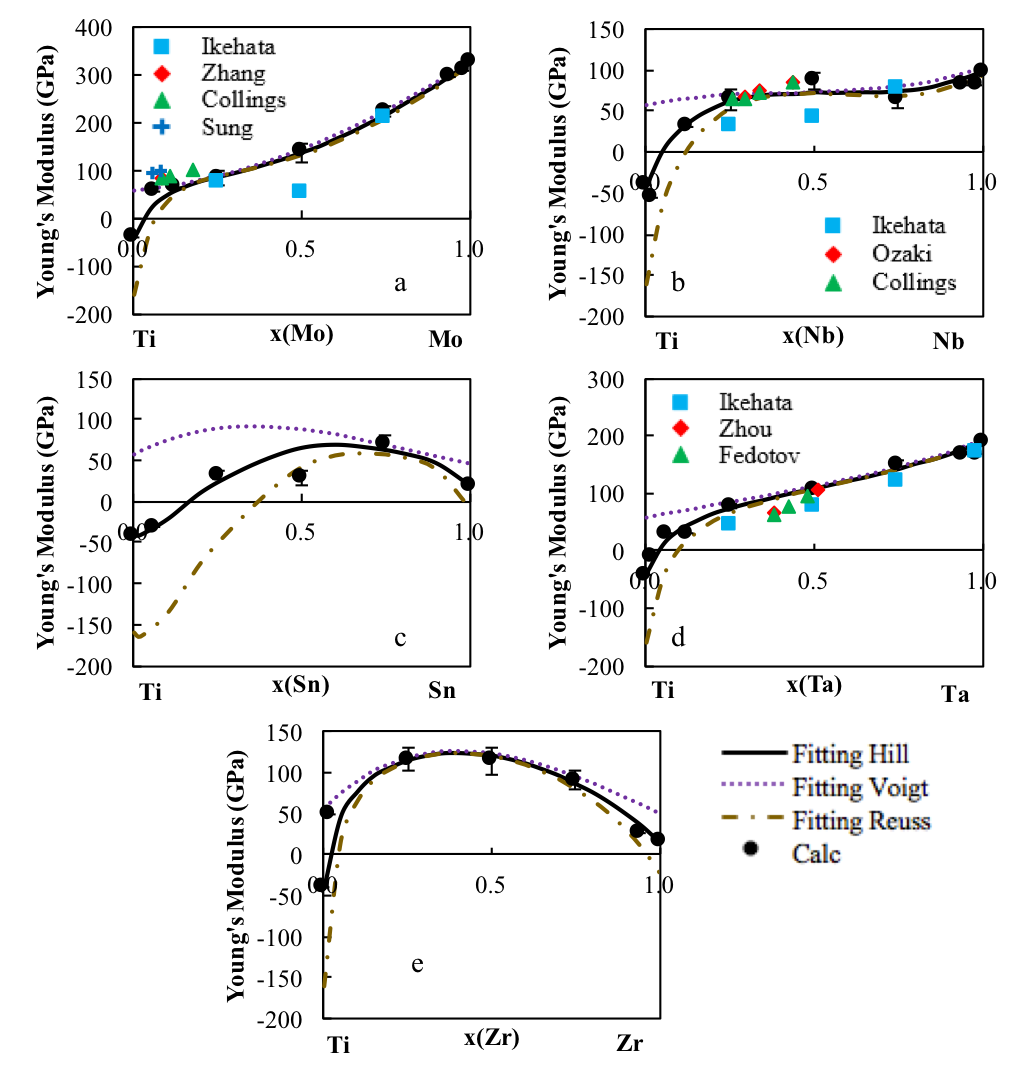
\includegraphics[width=\textwidth]{Chapter-5/Figures/tixyoungs.png}
	\caption{Young's modulus $E$ of the Ti-X binary systems. The present calculations are plotted as the filled circles with the error bars. The dotted purple line is the Voigt upper Young's modulus bound, the gold dot dashed line is the lower Reuss Young's modulus bound and the black line is the Hill Young's modulus average. The experimental values \cite{Ikehata2004,Zhang2015,Boyer1994,Sung2015,Ozaki2004,Fedotov1985,Zhou2009a,Zhou2004a,Friak2012,Wu2010a} are also included for comparison. }
	\label{Ch5-figure:tixyoungs}
\end{figure}

\pagebreak
\begin{figure}[H]
	\centering
	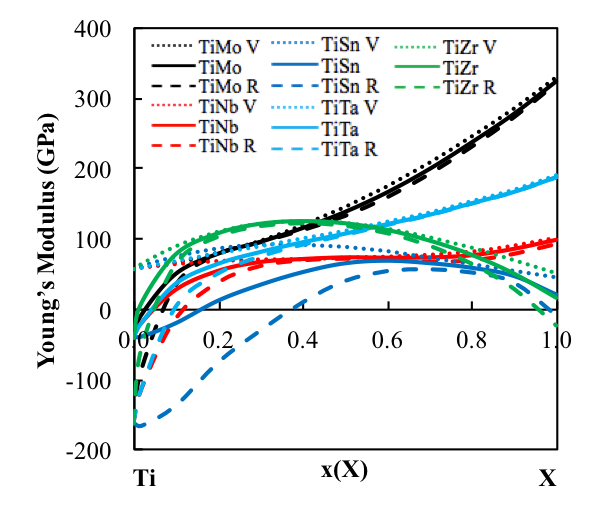
\includegraphics{Chapter-5/Figures/emap.png}
	\caption{Young's moduli mapped as a function of composition from bcc Ti to bcc X (X=Mo, Nb, Sn, Ta, Zr).}
	\label{Ch5-figure:tixmap}
\end{figure}

\pagebreak
\begin{figure}[H]
	\centering
	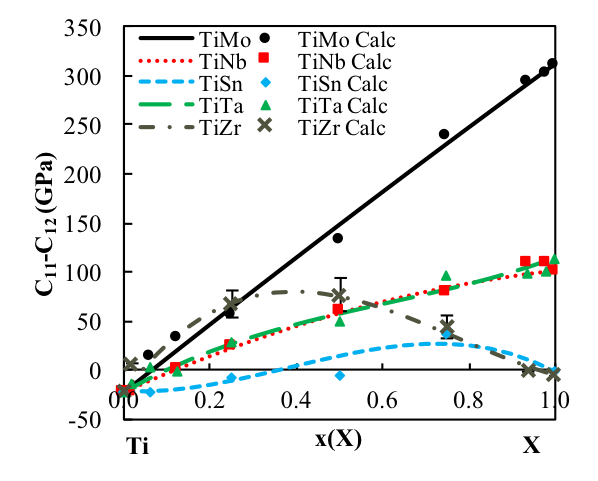
\includegraphics{Chapter-5/Figures/tixc11-c12.png}
	\caption{Calculated $\overline{C}_{11}$-$\overline{C}_{12}$ values (circles) plotted with the present modeling (solid lines) for five Ti-X binary systems (X = Mo, Nb, Ta, Sn, Zr). The $\overline{C}_{11}$-$\overline{C}_{12}$ shows the stability of the bcc phase. When the $\overline{C}_{11}$-$\overline{C}_{12}$ value is negative the bcc phase is not stable in the corresponding composition ranges.}
	\label{Ch5-figure:tixc11-c12}
\end{figure}

\pagebreak
\begin{figure}[H]
	\centering
	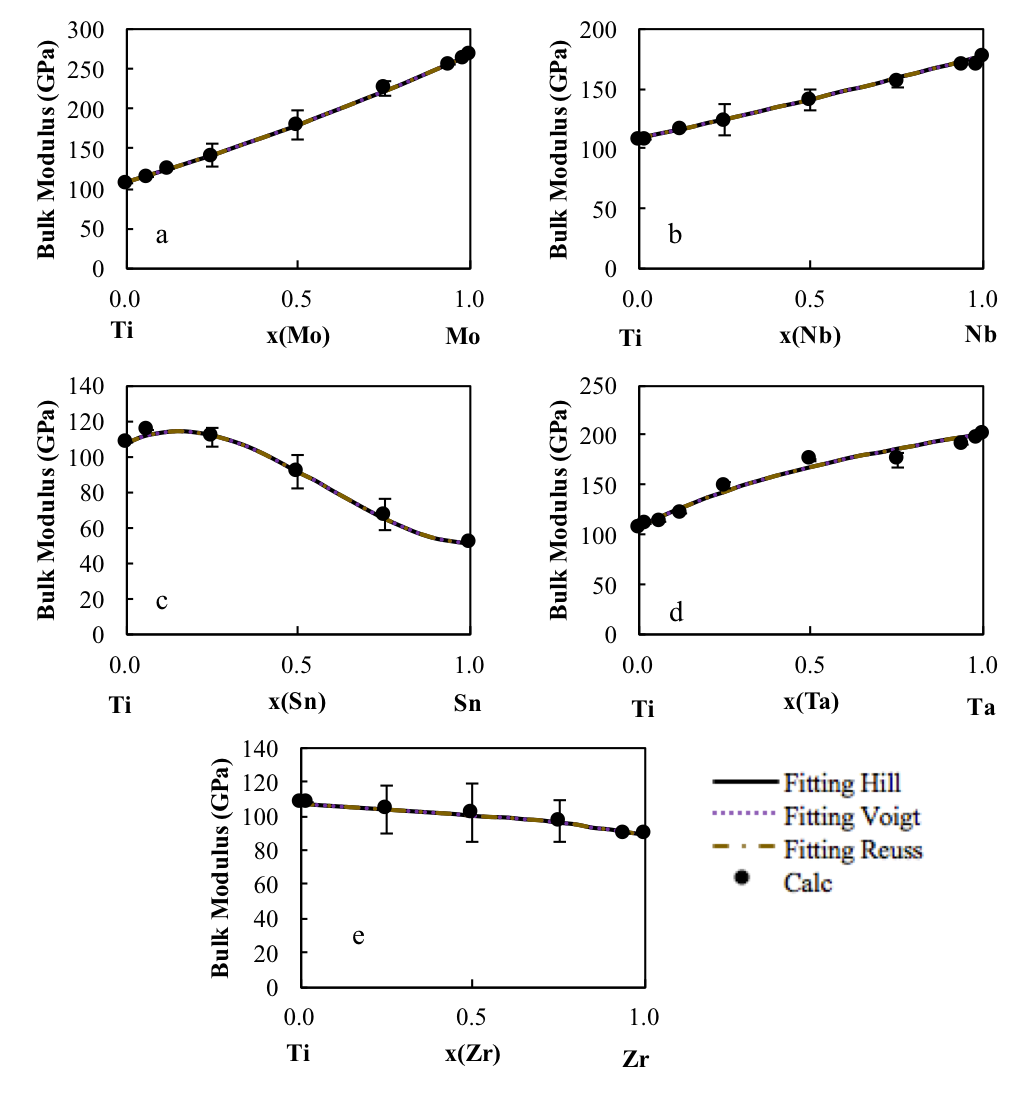
\includegraphics[width=\textwidth]{Chapter-5/Figures/tixbulk.png}
	\caption{Bulk moduli $B$ of the Ti-X binary systems. The present calculations are plotted as the filled circles with the error bars. The dotted purple line is the Voigt upper bulk modulus bound, the gold dot dashed line is the lower Reuss bulk modulus bound and the black line is the bulk modulus from the Hill approach.}
	\label{Ch5-figure:tixbulk}
\end{figure}

\pagebreak
\begin{figure}[H]
	\centering
	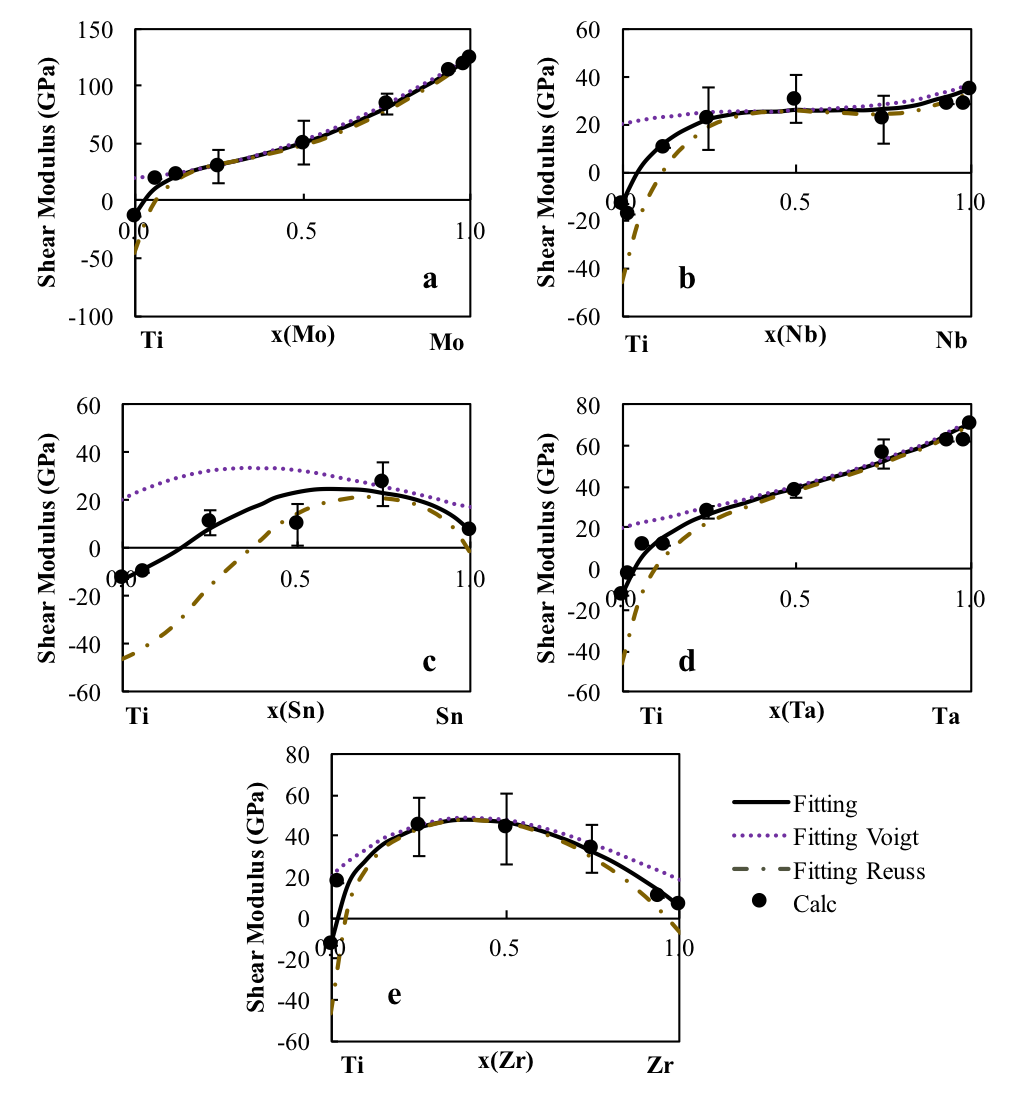
\includegraphics[width=\textwidth]{Chapter-5/Figures/tixshear.png}
	\caption{Shear moduli $G$ of the Ti-X binary systems. The present calculations are plotted as the filled circles with the error bars. The dotted purple line is the Voigt upper shear modulus bound, the gold dot dashed line is the lower Reuss shear modulus bound and the black line is the shear modulus from the Hill approach.}
	\label{Ch5-figure:tixshear}
\end{figure}

\pagebreak
\begin{figure}[H]
	\centering
	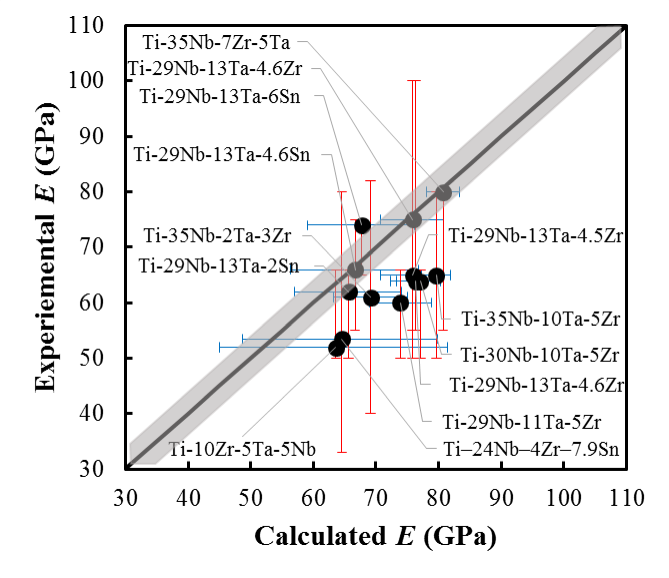
\includegraphics{Chapter-5/Figures/edatabase.png}
	\caption{Young's moduli values of multicomponent bcc Ti alloys measured experimentally plotted against the predicted Young's moduli from the pure elements and binary interaction parameters with the black diagonal line showing the exact correlation between the experimental and calculated values. Error in the experiments and the bounds from Reuss and Voigt approximations are plotted as the vertical and horizontal error bars, respectively. The variance in the first-principles calculations from Eq.\ref{eq: averagec11}-Eq.\ref{eq: averagec44} was averaged and plotted as the grey region. More information on the alloys is in Table \ref{Ch5-table:tixdatacomp} \cite{Tane2010a,Geetha2009,Mohammed2014}}
	\label{Ch5-figure:tixdatabase}
\end{figure}
\chapter{Effects of alloying elements on the elastic properties of bcc ternary and higher ordered Ti-alloys}

\section{Introduction}

In order to develop a better understanding about alloying effect on the elastic properties of Ti alloys, the present work is developing an elastic database for the Ti-Mo-Nb-Sn-Ta-Zr system. With the focus being on bcc Ti-alloys, the effects of alloying elements on the pure elements and Ti-X binary alloys in the bcc phase were calculated in chapter 5. After extrapolating to higher order systems, it was hypothesized that studying the effects of alloying on the elastic properties of ternary alloys would improve the database. The present work focuses on studying the elastic properties of the Ti-X-Y (X $\neq$Y = Mo, Nb, Ta, Sn, and Zr) ternary alloys in the bcc phase. The single crystal elastic stiffness constants (c$_{ij}$'s) and polycrystalline aggregate properties are predicted across the composition range using Density Functional Theory (DFT) at 0 $^\circ$K outlined in the methodology chapter. Based on the DFT results, the CALPHAD approach outlined in the methodology is used to evaluate ternary interaction parameters. The interaction parameters are then incorporated into the database and the database accuracy is again tested similarily to the testing in chapter 5. The completed database is used to map the elastic modulus as a function of compostion. 

\section{Modeling and Calculations}

\subsection{Calculation details}

To study the elastic properties of the ternary bcc Ti alloys in the Ti-Mo-Nb-Sn-Ta-Zr system, DFT-based first-principles calculations were employed using the VASP (Vienna ab-initio simulation package) \cite{Kresse1996,Kresse1999}. Four kinds of calculations were performed for each ternary alloy Ti-X-Y, with the varying compositions of X$_{50}$Y$_{50}$ (16-atom supercell), TiXY (36 atoms), Ti$_{2}$XY (32 atoms), Ti$_{6}$XY (64 atoms). The relaxation and use of SQS are discussed extensively in the methodology (chapter 2). The SQS used in this chapter were generated by Jiang et al. \cite{Jiang2004,Jiang2009}. The projector augmented wave (PAW) method was used to describe the ion-electron interaction. Based on our previous work done in chapter 5 (Figure \ref{Ch5-figure:PBEvsPW91}), the X-C functional of the generalized gradient approximation depicted by Perdew, Burke, and Ernzerhof (PBE-GGA) \cite{Perdew1996a} was employed. An energy cutoff roughly 1.3 times higher than the default values among all elements (i.e., 310 eV) was used for all calculations. The Brillouin zone sampling was done using the $\gamma$-centered Monkhorst-Pack scheme \cite{Monkhorst1976a}. The k-point grids used for the ternary SQS were 4x4x4 and the k-point grids used for the binary X50Y50 SQS structures were an automated k-point mesh generator in VASP with the length of the subdivision specified at 80. The elastic calculations were completed using a strain magnitude of $\pm$0.01 based on the study done in chapter 5 and the results seen in Figure \ref{Ch5-figure:Strain}.

\subsection{Modeling details}

The first-principles results were then used to model the ternary interaction parameters of the elastic stiffness constants. The modeling was completed by plotting the binary interpolation from the working database build in chapter 5. The plots started at a 50-50 mixture (X$_{50}$Y$_{50}$) of the alloying elements (X $\neq$ Y = Mo, Nb, Sn, Ta, and Zr) and plotted to pure Ti. The elastic stiffness constants of the pure elements and the binary interaction parameters from Table \ref{Ch5-table:tixelasip} were used to plot the binary interpolation. The differences between the ternary first-principles calculations and the binary interpolation were then used to obtain a single fitting parameter using the mathematica code in appendix C. With the focus being Ti-rich alloys and wanting to follow the same modeling technique used on the binary alloys, the first-principles results with 70 at.\% Ti or higher were weighted heavier (x6, according to the authors' practices) than the other points for the fittings. The best fit was found and the ternary interaction parameters were incorporated into the database. The databases was then used to predict the moduli values of the ternary and higher order alloys. 

\section{Results and discussion}

\subsection{Elastic calculation results}

The elastic stiffness constants $\overline{C}_{11}$, $\overline{C}_{12}$, and $\overline{C}_{44}$ are plotted in Figure \ref{Ch6-figure:tixyc11_1} to Figure \ref{Ch6-figure:tixyc44_2} for Ti-X-Y alloys (X $\neq$ Y = Mo, Nb, Sn, Ta, Zr). The plots start from a 50-50 mixture of the alloying elements X$_{50}$Y$_{50}$ to Ti. The calculations are plotted as circles, the interpolation from the pure elements and binary interaction parameters is plotted as a red dashed line. The difference between the calculations and binary interpolation was used to fit the ternary interaction parameters. The ternary fitting is plotted as a solid black line. The calculated elastic stiffness constants and moduli values are listed in Table \ref{Ch6-table:tixyelasdata} together with experimental values \cite{Niinomi2012,Mohammed2014,Nozoe2007,Geetha2009} for comparison.

The $\overline{C}_{11}$ values, for most of the Ti-X-Y systems, decrease from X$_{50}$Y$_{50}$ to Ti (see Figure \ref{Ch6-figure:tixyc11_1} and Figure \ref{Ch6-figure:tixyc11_2}). However, the Ti-Sn-Zr and Ti-Ta-Zr system differ. The  values, for the Ti-Sn-Zr (Figure \ref{Ch6-figure:tixyc11_2}d), first increase from Sn$_{50}$Zr$_{50}$ to 60 at.\% Ti and then decrease from 60 to 100 at.\% Ti. The  values, in the Ti-Ta-Zr system (Figure \ref{Ch6-figure:tixyc11_2}e), first increase from Ta$_{50}$Zr$_{50}$ to 35 at.\% Ti and then decrease from 35 to 100 at.\% Ti. The $\overline{C}_{12}$ results are plotted in Figure \ref{Ch6-figure:tixyc12_1} and Figure \ref{Ch6-figure:tixyc12_2}. The $\overline{C}_{12}$ values decrease from X$_{50}$Y$_{50}$ to Ti, for the Ti-Mo-Nb, Ti-Mo-Ta and Ti-Nb-Ta systems. The $\overline{C}_{12}$ values, for the Ti-Mo-Sn and Ti-Nb-Sn systems, first decrease from X$_{50}$Y$_{50}$ to 15 at.\% Ti then increase from 15 to 85 at.\% Ti and then decrease from 85 to 100 at.\% Ti. The Ti-Mo-Zr and Ti-Nb-Zr systems show a decrease in $\overline{C}_{12}$ value from X$_{50}$Y$_{50}$ to 60 at.\% Ti and then an increase from 60 to 100 at.\% Ti. The $\overline{C}_{12}$ values increase from X$_{50}$Y$_{50}$ to 70 at.\% Ti and then decrease from 70 to 100 at.\% Ti for the Ti-Sn-Ta system. For the Ti-Sn-Zr system, the$\overline{C}_{12}$ values increase from 0 to 100 at.\% Ti and the $\overline{C}_{12}$ values, for the Ti-Ta-Zr system, first decrease from 0 to 70 at.\% Ti and then increase from 70 to 100 at.\% Ti. The $\overline{C}_{44}$ results are plotted in Figure \ref{Ch6-figure:tixyc44_1} and Figure \ref{Ch6-figure:tixyc44_2}. The $\overline{C}_{44}$ values decrease from X$_{50}$Y$_{50}$ to Ti, for the Ti-Mo-Sn and Ti-Ta-Zr systems. For the Ti-Mo-Zr and Ti-Mo-Ta systems, the $\overline{C}_{44}$ values first decrease from 0 to 80 at.\% Ti and then increase from 80 to 100 at.\% Ti. The $\overline{C}_{44}$ values, for the Ti-Mo-Nb and Ti-Nb-Ta systems, first decrease from X$_{50}$Y$_{50}$ to 65 at.\% Ti and then increase from 65 to 100 at.\% Ti. The $\overline{C}_{44}$ values first increase from 0 to 80 at.\% Ti and then decrease from 80 to 100 at.\% Ti for the Ti-Nb-Sn and Ti-Nb-Zr systems. For the Ti-Sn-Ta system (Figure \ref{Ch6-figure:tixyc44_2}c), the $\overline{C}_{44}$ values decrease from 0 until 20 at.\% Ti, then increase from 20 to 50 at.\% Ti and then decrease from 50 to 100 at.\% Ti. The $\overline{C}_{44}$ values, for the Ti-Sn-Zr system, first increase from X$_{50}$Y$_{50}$ to 60 at.\% Ti and then decrease from 60 to 100 at.\% Ti.

The trends in the ternary elastic stiffness constants can be summarized and explained by looking at the elastic stiffness calculations done on the pure elements and Ti-X (X = Mo, Nb, Sn, Ta, Zr) Chapter 5. The c$_{11}$ and c$_{12}$ of Mo, Nb and Ta are higher than Ti, while Sn and Zr are lower. The c$_{44}$ for Mo and Ta are higher than Ti, while Nb, Sn, and Zr are lower. This can be explained because Mo, Nb and Ta are stable in the bcc structure at low temperatures while Ti, Sn and Zr are not, so the elastic stiffness constants are lower. The similarities of Mo, Nb and Ta are again noticed in the Ti-X data trends. The $\overline{C}_{11}$, $\overline{C}_{12}$, and $\overline{C}_{44}$ all follow the same trends for the Ti-Mo, Ti-Nb, and Ti-Ta systems with the $\overline{C}_{11}$ and $\overline{C}_{12}$ increasing in value from 100 to 0 at.\% Ti and the $\overline{C}_{44}$ decreases and then increases from 100 to 0 at.\% Ti. Based on this information, it is no surprise that the Ti-Mo-Nb, Ti-Mo-Ta and Ti-Nb-Ta systems have the same trends in their c$_{ij}$ data. When Ti-Mo, Ti-Nb, and Ti-Ta are alloyed with Sn in the ternary systems, they show similar trends for the most, not all, of the c$_{ij}$. The same is true for the Ti-Mo, Ti-Nb, and Ti-Ta systems alloyed with Zr.

Based on the discussion in the methodology, Born's criteria is used to look at the mechanical stability of the bcc phase. When $\overline{C}_{11}$-$\overline{C}_{12}$ becomes negative then the bcc phase loses mechanical stability and is thus plotted in Figure \ref{Ch6-figure:tixyc11-c12}. Based on the present results, the bcc phase loses mechanical stability in the Ti-Mo-Nb, Ti-Mo-Ta, Ti-Mo-Zr, Ti-Nb-Zr, Ti-Sn-Zr, and Ti-Ta-Zr systems when the Ti concentration is more than 90 at.\%, with the values being 91, 92, 95, 93, 91, and 94 at.\% Ti, respectively. The bcc phase loses mechanical stability at Ti concentrations above 87, 77, 89, and 80 at.\% Ti for Ti-Mo-Sn, Ti-Nb-Sn, Ti-Nb-Ta and Ti-Sn-Ta systems, respectively. Close to where the bcc phase loses its mechanical stability, the Young's modulus is reduced and such compositions may be desirable low modulus bcc Ti alloys.

Figure \ref{Ch6-figure:tixyyoungs1} and Figure \ref{Ch6-figure:tixyyoungs2} plot the Young's moduli ($E$) calculations (circles) for each Ti-X-Y ternary system (X $\neq$ Y = Mo, Nb, Sn, Ta, Zr) starting from a 50-50 mixture of the two alloying elements to Ti. The red dashed line is the Hill average interpolated from the binary interaction parameters shown in Table \ref{Ch5-table:tixelasip}. The Hill average (black solid line), Voigt (purple dotted line), Reuss (gold dotted-dashed line) bounds are plotted using the binary (Table \ref{Ch5-table:tixelasdata})and ternary interaction parameters (Table \ref{Ch6-table:tixyelasip}). The Voigt and Reuss bounds vary more drastically when the bcc structure is unstable as opposed to when the bcc structure is stable. The Hill average with the binary and ternary interaction parameters is employed, which should be closer to the polycrystalline values. The Hill average is what the database predicts because it has been shown to be a more accurate representation of the Young's modulus \cite{Yue2009,Chung1967}. Whenever possible experimentally determined Young's moduli \cite{Niinomi2012,Mohammed2014,Nozoe2007,Geetha2009} (data listed in Table \ref{Ch6-table:tixyelasdata}) are plotted for comparison. The difference/error between the previous results (both experimental and from calculations) and the present first-principles results is reported here. The equation is defined in Chapter 2 Eq. \ref{eq: error}.

The first-principles $E$, for the Ti-Mo-Nb (Figure \ref{Ch6-figure:tixyyoungs1}a) system are compared with experimentally obtained $E$ data in the review paper by Niinomi et al. \cite{Niinomi2012}. The experimental $E$ results were obtained using a nanoindenter after solution treatment. The experimental $E$ values are higher than the Hill average calculated values (difference of 71 GPa or an error of 0.65 using Eq. \ref{eq: error}) and more closely match the Voigt bound (difference of 46 GPa). Niinomi \cite{Niinomi2012} pointed out that Young's moduli obtained from microhardness testing are higher than the polycrystalline Young's moduli value, thus our calculation results should be close to the polycrystalline $E$ values. The present data show that the $E$ decreases in value from 0 to 100 at.\% Ti. 

In the literature, no bcc Ti-Mo-Sn (Figure \ref{Ch6-figure:tixyyoungs1}b) experimental $E$ results were found to be compared with the present work. The Voigt-Reuss bounds and the Hill average are quite similar until around 65 at.\% Ti when they begin to vary. The $E$ values decrease from 0 to 100 at.\% Ti. The calculated E results for the Ti-Mo-Ta alloy system (Figure \ref{Ch6-figure:tixyyoungs1}c) are compared with experimental data reported by Niinomi et al. \cite{Niinomi2012} and Mohammed et al. \cite{Mohammed2014}. The $E$ values reported by Niinomi et al. \cite{Niinomi2012} were obtained using an ultrasonic measurement after the samples were solution treated. Niinomi et al. \cite{Niinomi2012} pointed out that the ultrasonic method obtained $E$ values in between the tensile test and microhardness methodology and showed no large error in the experiments. The experimental $E$ fit well with the present Voigt bound (difference of 9 GPa) and had an error of 0.46 (Eq. \ref{eq: error}) from the Hill average (difference of 33 GPa). The $E$ values decrease from 0 to 100 at.\% Ti. 

The Young's moduli of the Ti-Mo-Zr alloy system (Figure \ref{Ch6-figure:tixyyoungs1}d) is compared with experimental values reported by Mohammed et al. \cite{Mohammed2014}. The error in the experiments and methodology was not discussed. The experimental $E$ \cite{Mohammed2014} and the present $E$ (Hill average) vary by less than 6 GPa and the $E$ values decrease from 0 to 100 at.\% Ti. Experimentally determined Young's modli results from Niinomi et al. \cite{Niinomi2012}, Mohammed et al. \cite{Mohammed2014}, and Nozoe et al. \cite{Nozoe2007} are compared with the present $E$ calculations for the Ti-Nb-Sn alloy system (Figure \ref{Ch6-figure:tixyyoungs1}e). The experimental $E$ results reported by Niinomi et al. \cite{Niinomi2012} were obtained through tensile testing of samples that were solution treated and cold rolled. Niinomi et al. showed that $E$ results at this specific composition varied by 10 GPa. The $E$ results reported by Niinomi et al. \cite{Niinomi2012} and Mohammed et al. \cite{Mohammed2014} differ from the Hill average by 9 and 15 GPa, respectively (an error of 0.28 using Eq. \ref{eq: error}). The $E$ results from Nozoe et al. \cite{Nozoe2007} differ by 10, 32 and 78 GPa from the Voigt, Hill and Reuss results, respectively, and have an error of 0.56 (Eq. \ref{eq: error}). However, Nozoe et al. reported that the samples formed the metastable omega phase. The $\omega$ phase is a metastable hexagonal phase (space group P6/mmm) with lattice parameters closely matching those of the bcc phase. Nozoe et al. \cite{Nozoe2007} also discussed how the aging of the Ti-Mo-Sn samples greatly affected the $E$. So overall the calculations satisfactorily predicted the Young's moduli of the Ti-Mo-Nb, Ti-Mo-Sn, Ti-Mo-Ta, Ti-Mo-Zr and Ti-Nb-Sn systems. 

Figure \ref{Ch6-figure:tixyyoungs2} continues to plot the $E$ of the Ti-X-Y ternary alloy systems. The first-principles $E$, for the Ti-Nb-Ta system, are compared with experimentally determined $E$ values reported by Mohammed et al. \cite{Mohammed2014} (Figure \cite{Mohammed2014}a). At this composition, the Voigt and Reuss bounds are very close to the Hill average. Thus, while the experimental $E$ result fits closer to the Reuss bound (difference of 8 GPa), the experimental $E$ result only varies by 15 and 21 GPa from the Hill and Voigt results, respectively and has an error of 0.28 (Eq. \ref{eq: error}). Niinomi et al. \cite{Niinomi2012} reported the $E$ results of a different composition Ti-Nb-Ta alloy, Ti-29Nb-13Ta as opposed to Ti-25Nb-25Ta. Niinomi et al. \cite{Niinomi2012} showed that the $E$ determined experimentally for the Ti-Nb-Ta alloy varies by approximately 40 GPa. The $E$ decreases in value from 0 to 100 at.\% Ti in the Ti-Nb-Ta ternary system. 

The first-principles $E$ results for the Ti-Nb-Zr (Figure \ref{Ch6-figure:tixyyoungs2}b) system are compared with experimentally determined $E$ results from Geetha et al. \cite{Geetha2009},  Mohammed et al. \cite{Mohammed2014}, and Niinomi et al. \cite{Niinomi2012}. The experimental $E$ results reported by Niinomi et al. \cite{Niinomi2012} are for the Ti-13Nb-13Zr and Ti-27Nb-8Zr alloys. The results for the Ti-13Nb-13Zr were obtained using both the ultrasonic and 3-point bending tests and varied by 50 GPa, while the Ti-27Nb-8Zr results were obtained using tensile testing and varied by 50 GPa. The experimentally determined $E$ results varied from the present Voigt, Hill and Reuss results by an average of 9, 2, and 14 GPa, respectively and has an error of 0.08 (Eq. \ref{Ch6-figure:tixyyoungs2}) from the Hill average. Overall, the $E$ first increases in value from 0 to 70 at.\% Ti and then decreases from 70 to 100 at.\% Ti for the Ti-Nb-Zr system. The Ti-Sn-Ta, Ti-Sn-Zr and Ti-Ta-Zr alloy systems have experimental data to be compared with and our results are shown in Figure \ref{Ch6-figure:tixyyoungs2}c, Figure \ref{Ch6-figure:tixyyoungs2}d, and Figure \ref{Ch6-figure:tixyyoungs2}e, respectively. For the Ti-Sn-Ta system, the $E$ values decreases in value from 0 to 100 at.\% Ti. The $E$ values for the Ti-Sn-Zr system first increases from 0 to 60 at.\% Ti and then decreases from 60 to 100 at.\% Ti. The $E$ values for the Ti-Ta-Zr system first decreases from 0 to 15 at.\% Ti, where the values begin to increase from 15 to 30 at.\% Ti and then decreases from 30 to 100 at.\% Ti. 

It can be seen that there is a large variation in the experimental data depending on the technique used to obtain the data. Also, the first-principles calculations and the CALPHAD fittings are done using data obtained at 0 $^{\circ}$K while the experiments are obtained using polycrystalline samples at 300 $^{\circ}$K. Considering these facts, the experimental values fit well within the bounds set by Reuss and Voigt, and the Hill average generally reproduces the experimentally determined $E$ data for the Ti-X-Y ternary alloys. 

Using the complete database with interaction parameters listed in Table \ref{Ch5-table:tixelasip} and \ref{Ch6-table:tixyelasip}, the elastic stiffness constants can be predicted and then the moduli values can be calculated and mapped. Figure \ref{Ch6-figure:tixymap1} and Figure \ref{Ch6-figure:tixymap2} uses the global minimization tools in pycalphad \cite{Otis2017} to map the $E$ based on composition for Ti-X-Y ternaries. The maps can point to regions with specific moduli values to be targeted. The pycalphad code used is in appendix E.

The $B$ and $G$ moduli calculated (circles) are plotted in Figure \ref{Ch6-figure:tixybulk1} to Figure \ref{Ch6-figure:tixyshear2} for each Ti-X-Y (X $\neq$ Y = Mo, Nb, Sn, Ta, Zr) system starting from a 50-50 mixture of X and Y to Ti. The red dashed line is the Hill average interpolated from the binary interaction parameters shown in Table \ref{Ch5-table:tixelasip}. The Hill average (black solid line), Voigt (purple dotted line), Reuss (gold dotted-dashed line) bounds are plotted using the binary and ternary interaction parameters (Table \ref{Ch5-table:tixelasip} and \ref{Ch6-table:tixyelasip}). The $B$ values, for all the Ti-X-Y ternaries except Ti-Nb-Sn, Ti-Sn-Ta and Ti-Sn-Zr decreases from 0 to 100 at.\% Ti, as shown in Figure \ref{Ch6-figure:tixybulk1} and Figure \ref{Ch6-figure:tixybulk2}. The $B$ values for the Ti-Nb-Sn and Ti-Sn-Ta systems first decrease from 0 to 10 at.\% Ti and then increase from 10 to 55 at.\% Ti and then decrease from 55 to 100 at.\% Ti. For the Ti-Sn-Zr system, the $B$ values first increase from 0 to 85 at.\% Ti and then decreases from 85 to 100 at.\% Ti. The $G$ values decrease from 0 to 100 at.\% Ti for all the ternary systems except Ti-Nb-Sn, Ti-Nb-Zr, Ti-Sn-Zr and Ti-Ta-Zr (Figure \ref{Ch6-figure:tixyshear1} and Figure \ref{Ch6-figure:tixyshear2}). The $G$ values increase from 0 to 60 at.\% Ti and then decrease from 60 to 100 at.\% Ti for the Ti-Nb-Sn, Ti-Nb-Zr systems. For the Ti-Sn-Zr system, the $G$ values first increase from 0 to 55 at.\% Ti and then decrease from 55 to 100 at.\% Ti. The $G$ values increase from 0 to 40 at.\% Ti and then decrease from 40 to 100 at.\% Ti for the Ti-Ta-Zr system. 

Both the $G$ and $E$ are negative when they are close to Ti. This is due to the instability of the bcc phase close to Ti. As discussed by Born’s criteria, when $\overline{C}_{11}$-$\overline{C}_{12}$ is negative the bcc phase loses mechanical stability. The Voigt bound of $G_{v}$ is expressed by:

%%
\begin{equation}
\label{eq: Gv}
G_v = \left( \overline{C}_{11}-\overline{C}_{12}+\overline{C}_{44} \right)/5
\end{equation}
%%

So, when $\overline{C}_{11}$-$\overline{C}_{12}$ it causes $G$ to be negative. The $E$ is then calculated from the $B$ and $G$, so when $G$ is negative it can cause $E$ to be negative. This is one of the reasons that finding bcc Ti alloys close to the bcc stability will produce a low $E$. 



\subsection{Extrapolation to higher ordered systems}

The pure element elastic results along with the binary and ternary interaction parameters are combined into a database file in appendix D. The $E$ is predicted and compared with experimental results for higher order Ti alloys and the results are shown in Table \ref{Ch6-table:tixydatacomp} and Figure \ref{Ch6-figure:tixydatabase}. The same comparison was made in chapter 5 (Table \ref{Ch5-table:tixdatacomp} and Figure \ref{Ch5-table:tixdatacomp}), but those predictions were made without the ternary interaction parameters. Figure \ref{Ch6-figure:tixydatabase} plots the calculated $E$ (Hill average) versus the experimentally determined Young's moduli \cite{Tane2010a,Mohammed2014,Geetha2009}. The black diagonal line would be a perfect correlation between the predictions and experiments. The grey region is the average variance in the first-principles calculations when calculating the average elastic stiffness constants using Eq. \ref{eq: averagec11}-Eq. \ref{eq: averagec44} (3 GPa). The same higher order alloys were picked to compare the effect of introducing the ternary interaction parameters. As discussed previously, the error bars plotted for the experiments come from the variance that was seen when comparing the experimentally determined Young's moduli at the same composition from Niinomi et al. \cite{Niinomi2012}, Geetha et al. \cite{Geetha2009}, Tane et al. \cite{Tane2010a}, and Mohammed et al. \cite{Mohammed2014}. The horizontal error bars are the Voigt and Reuss bounds. Previously, without ternary interaction parameters, the predictions and experimental results varied anywhere between 0.69 and 14 GPa and on average by 7 GPa. The calculations are usually larger than the experimental values due to the temperature difference: the computed single crystal elastic stiffness constants are at 0 $^{\circ}$K, while the experiments on the polycrystalline samples are usually performed at 300 $^{\circ}$K. As discussed, introducing ternary interaction parameters improves the database. The introduction of the ternary interaction parameters improved the predictions to vary anywhere from 0.39 to 13 GPa from the experimental values with an average variance of only 5 GPa. Thus, while the ternary interactions have small effects on the final results, the introduction of Ti-containing ternary interaction parameters still improves the predictions and the database is more accurate to predict the Young's modulus of higher order Ti alloys. 

\section{Conclusion}

The present study systematically calculates the elastic properties of the bcc Ti ternary alloys, including the elastic stiffness constants, bulk modulus, shear modulus, and Young's modulus. Five alloying elements, Mo, Nb, Sn, Ta and Zr are studied. The general CALPHAD modeling approach is used to fit ternary interaction parameters. From the elastic stiffness constant data, the Ti-X-Y (X $\neq$ Y = Mo, Nb, Ta) show the same trends in the data. This is to be expected because Mo, Nb, and Ta are similar elements that are strong $\beta$-stabilizers and stable in the bcc phase at low temperatures. It was also seen that the Ti-X-Sn (X = Mo, Nb, Ta) alloys showed similar trends in the data for most of the elastic stiffness constants, so do the Ti-X-Zr (X = Mo, Nb, Ta) alloys. The present calculations showed that the bcc Ti-alloy was mechanically stabilized at compositions less than 91, 92, 95, 93, 91, 94, 87, 77, 89, and 80 at \% Ti for the Ti-Mo-Nb, Ti-Mo-Ta, Ti-Mo-Zr, Ti-Nb-Zr, Ti-Sn-Zr, Ti-Ta-Zr, Ti-Mo-Sn, Ti-Nb-Sn, Ti-Nb-Ta and Ti-Sn-Ta alloys, respectively. As discussed above, Mo, Nb and Ta are strong $\beta$-stabilizers and thus the Ti-Mo-Nb, Ti-Mo-Ta, and Ti-Nb-Ta systems stabilize the bcc phase similarly. Also, discussed previously, Zr is a weak $\beta$-stabilizer alone but when alloyed with other elements it acts a strong $\beta$-stabilizer. This is observed with these results with the Ti-Mo-Zr, Ti-Nb-Zr, Ti-Ta-Zr systems all stabilizing the bcc phase at high Ti concentrations (95, 93, and 94 at.\% respectively). Zr is even able to stabilize the Ti-Sn-Zr system at a high Ti concentration of 91 at.\% Ti, even with Sn. Sn is not stable in the bcc phase and is not a $\beta$-stabilizer. So, when alloyed with Sn, a higher concentration of other alloying elements is needed to stabilize the bcc phase. 

The pure element elastic results along with the binary and ternary interaction parameters are combined into a database file in appendix D. The database can be used to map possible alloy compositions to find potential materials with a Young's modulus in the target range for biomedical load-bearing implants using the pycalphd code in appendix e. Overall, the introduction of the ternary interaction parameters improved the database's ability to predict the $E$ of higher order alloys by a small amount. The complete database, however, satisfactorily predicts the elastic properties of higher order Ti-alloys and will help guide future research to develop low-modulus biocompatible Ti alloys.

\newpage
\begin{longtable}[H]{ c c c c c}
	\caption{First-principles calculations of the elastic stiffness constants} 	\label{Ch6-table:tixyecijdata} \\
	\hline
	Reference & Ti$_{100-2b}$X$_b$Y$_b$ & $\overline{C}_{11}$ & $\overline{C}_{11}$ & $\overline{C}_{11}$ \\
	\hline
	\endhead
	\hline
	\endfoot
	This work & Ti & 93 & 115 & 41 \\
	This work & TiMo$_{12.5}$Nb$_{12.5}$ & 155 & 121 $\pm$4 & 34 $\pm$4 \\
	This work & TiMo$_{25.0}$Nb$_{25.0}$ & 222 $\pm$3 & 129 $\pm$3 & 33 $\pm$3 \\
	This work & TiMo$_{33.3}$Nb$_{33.3}$ & 269 $\pm$5 & 134 $\pm$3 & 42 $\pm$4 \\
	This work & Mo$_{50}$Nb$_{50}$ & 414 $\pm$6 & 165 $\pm$3 & 68 \\
	This work & TiMo$_{12.5}$Sn$_{12.5}$ & 137 $\pm$15 & 121 $\pm$2 & 56 $\pm$13 \\
	This work & TiMo$_{25.0}$Sn$_{25.0}$ & 160 $\pm$3 & 130 $\pm$8 & 71 $\pm$2 \\
	This work & TiMo$_{33.3}$Sn$_{33.3}$ & 167 $\pm$8 & 133 $\pm$6 & 75 $\pm$2 \\
	This work & Mo$_{50}$Sn$_{50}$ & 192 $\pm$28 & 130 $\pm$36 & 40 $\pm$31 \\
	This work & TiMo$_{12.5}$Ta$_{12.5}$ & 153 $\pm$1 & 125 $\pm$4 & 38 $\pm$3 \\
	This work & TiMo$_{25.0}$Ta$_{25.0}$ & 222 $\pm$2 & 136 $\pm$1 & 45 $\pm$3 \\
	This work & TiMo$_{33.3}$Ta$_{33.3}$ & 263 $\pm$4 & 145 $\pm$6 & 49 $\pm$4 \\
	This work & Mo$_{50}$Ta$_{50}$ & 370 $\pm$13 & 163 $\pm$4 & 63 $\pm$4 \\
	This work & TiMo$_{12.5}$Zr$_{12.5}$ & 125 $\pm$1 & 109 $\pm$8 & 35 $\pm$1 \\
	This work & TiMo$_{25.0}$Zr$_{25.0}$ & 160 $\pm$1 & 116 $\pm$5 & 34 $\pm$2 \\
	This work & TiMo$_{33.3}$Zr$_{33.3}$ & 182 $\pm$1 & 116 $\pm$2 & 31 $\pm$8 \\
	This work & Mo$_{50}$Zr$_{50}$ & 231 $\pm$7 & 118 $\pm$5 & 33 $\pm$8 \\
	This work & TiNb$_{12.5}$Sn$_{12.5}$ & 115 $\pm$4 & 118 $\pm$3 & 55 \\
	This work & TiNb$_{25.0}$Sn$_{25.0}$ & 131 $\pm$9 & 121 $\pm$6 & 64 $\pm$3 \\
	This work & TiNb$_{33.3}$Sn$_{33.3}$ & 134 $\pm$2 & 122 $\pm$3 & 67 $\pm$6 \\
	This work & Nb$_{50}$Sn$_{50}$ & 132 $\pm$4 & 118 $\pm$8 & 56 $\pm$4 \\
	This work & TiNb$_{12.5}$Ta$_{12.5}$ & 130 $\pm$3 & 124 $\pm$4 & 37 $\pm$3 \\
	This work & TiNb$_{25.0}$Ta$_{25.0}$ & 182 $\pm$1 & 129 $\pm$4 & 43 $\pm$6 \\
	This work & $_{33.3}$Ta$_{33.3}$ & 208 & 135 $\pm$1 & 44 $\pm$1 \\
	This work & Nb$_{50}$Ta$_{50}$ & 260 $\pm$2 & 148 $\pm$3 & 47 $\pm$3 \\
	This work & TiNb$_{12.5}$Zr$_{12.5}$ & 101 $\pm$2 & 113 $\pm$4 & 32 $\pm$3\\
	This work & TiNb$_{25.0}$Zr$_{25.0}$ & 122 $\pm$1 & 113 $\pm$3 & 28 $\pm$3 \\
	This work & TiNb$_{33.3}$Zr$_{33.3}$ & 143 $\pm$2 & 107 $\pm$5 & 28 $\pm$3 \\
	This work & Nb$_{50}$Zr$_{50}$ & 154 $\pm$5 & 110 $\pm$3 & 15 $\pm$2 \\
	This work & TiSn$_{12.5}$Ta$_{12.5}$ & 115 $\pm$6 & 121 $\pm$4 & 60 $\pm$2 \\
	This work & TiSn$_{25.0}$Ta$_{25.0}$ & 138 $\pm$13 & 125 $\pm$4 & 75 $\pm$4 \\
	This work & TiSn$_{33.3}$Ta$_{33.3}$ & 138 $\pm$6 & 131 $\pm$8 & 78 $\pm$1 \\
	This work & Sn$_{50}$Ta$_{50}$ & 133 $\pm$8 & 130 $\pm$4 & 60 $\pm$4 \\
	This work & TiSn$_{12.5}$Zr$_{12.5}$ & 97 $\pm$5 & 111 $\pm$4 & 55 $\pm$2 \\
	This work & TiSn$_{25.0}$Zr$_{25.0}$ & 99 $\pm$12 & 103 $\pm$4 & 59 $\pm$7 \\
	This work & TiSn$_{33.3}$Zr$_{33.3}$ & 96 $\pm$7 & 98 $\pm$3 & 55 $\pm$3 \\
	This work & Sn$_{50}$Zr$_{50}$ & 85 $\pm$7 & 87 $\pm$9 & 42 $\pm$3 \\
	This work & TiTa$_{12.5}$Zr$_{12.5}$ & 136 $\pm$36 & 103 $\pm$21 & 44 $\pm$5 \\
	This work & TiTa$_{25.0}$Zr$_{25.0}$ & 130 $\pm$3 & 117 $\pm$4 & 42 $\pm$7 \\
	This work & TiTa$_{33.3}$Zr$_{33.3}$ & 148 $\pm$1 & 115 $\pm$2 & 44 $\pm$2 \\
	This work & Ta$_{50}$Zr$_{50}$ & 157 $\pm$2 & 123 $\pm$3 & 35 $\pm$3 \\
	\hline
\end{longtable}
%%%

\newpage
\begin{longtable}[H]{ c c c c c }
	\caption{First-principles calculations of the bulk modulus $B$, shear modulus $G$, and Young's modulus $E$ in GPa for different atomic percent compositions of the bcc Ti-X-Y ternary systems at 0 $^{\circ}$K as well as experimental data obtained for the Young's modulus at 300 $^{\circ}$K by the references stated.} 	\label{Ch6-table:tixyelasdata} \\
	\hline
	Reference & Ti$_{100-2b}$X$_b$Y$_b$ & $B$ &$G$ & $E$\\
	\hline
	\endhead
	\hline
	\endfoot
	This work & Ti & 108 & -12.91 & -40.34\\
	This work & TiMo$_{12.5}$Nb$_{12.5}$ & 132 $\pm$4 & 26 $\pm$4 & 73 $\pm$4\\
	This work & TiMo$_{25.0}$Nb$_{25.0}$ & 160 $\pm$3 & 38 $\pm$3 & 105 $\pm$3\\
	This work & TiMo$_{33.3}$Nb$_{33.3}$ & 179 $\pm$5 & 51 $\pm$5 & 139 $\pm$5\\
	This work & Mo$_{50}$Nb$_{50}$ & 248 $\pm$6 & 87 $\pm$6 & 233 $\pm$6\\
	Expt 300 K \cite{Niinomi2012} & TiMo$_{6}$Nb$_{2}$ & & & 110\\
	This work & TiMo$_{12.5}$Sn$_{12.5}$ & 126 $\pm$15 & 27 $\pm$15 & 75 +$\pm$15\\
	This work & TiMo$_{25.0}$Sn$_{25.0}$ & 140 $\pm$8 & 39 $\pm$8 & 106 $\pm$8\\
	This work & TiMo$_{33.3}$Sn$_{33.3}$ & 144 $\pm$8 & 42 $\pm$8 & 114 $\pm$8\\
	This work & Mo$_{50}$Sn$_{50}$ & 151 $\pm$36 & 36 $\pm$36 & 100 $\pm$36\\
	This work & TiMo$_{12.5}$Ta$_{12.5}$ & 134 $\pm$4 & 25 $\pm$4 & 72 $\pm$4\\
	This work & TiMo$_{25.0}$Ta$_{25.0}$ & 165 $\pm$2 & 44 $\pm$3 & 122 $\pm$3\\
	This work & TiMo$_{33.3}$Ta$_{33.3}$ & 184 $\pm$6 & 53 $\pm$6 & 145 $\pm$\\
	This work & Mo$_{50}$Ta$_{50}$ & 232 $\pm$13 & 77 $\pm$13 & 208 $\pm$13\\
	Expt 300 K \cite{Mohammed2014} & TiMo$_{7}$Ta$_{1}$ & & & 74\\
	Expt 300 K \cite{Niinomi2012}  & TiMo$_{7}$Ta$_{1}$ & & & 74\\
	This work & TiMo$_{12.5}$Zr$_{12.5}$ & 114 $\pm$8 & 20 $\pm$8 & 55 $\pm$8\\
	This work & TiMo$_{25.0}$Zr$_{25.0}$ & 131 $\pm$5 & 29 $\pm$5 & 80 $\pm$5\\
	This work & TiMo$_{33.3}$Zr$_{33.3}$ & 138 $\pm$2 & 32 $\pm$8 & 89 $\pm$8\\
	This work & Mo$_{50}$Zr$_{50}$ & 156 $\pm$7 & 41 $\pm$8 & 113 $\pm$8\\
	Expt 300 K \cite{Mohammed2014} & TiMo$_{7}$Zr$_{3}$ & & & 64\\
	This work & TiNb$_{12.5}$Sn$_{12.5}$ & 117 $\pm$4 & 14 $\pm$4 & 41 $\pm$4\\
	This work & TiNb$_{25.0}$Sn$_{25.0}$ & 124 $\pm$9 & 26 $\pm$9 & 72 $\pm$9\\
	This work & TiNb$_{33.3}$Sn$_{33.3}$ & 126 $\pm$6 & 28 $\pm$6 & 78 $\pm$6\\
	This work & Nb$_{50}$Sn$_{50}$ & 123 $\pm$8 & 26 $\pm$8 & 72 $\pm$8\\
	Expt 300 K \cite{Mohammed2014} & TiNb$_{22}$Sn$_{2}$ & & & 44\\
	Expt 300 K \cite{Niinomi2012} & TiNb$_{22}$Sn$_{2}$ & & & 50\\
	Expt 300 K \cite{Nozoe2007} & TiNb$_{9}$Sn$_{3}$ & & & 58\\
	This work & TiNb$_{12.5}$Ta$_{12.5}$ & 126 $\pm$4 & 15 $\pm$4 & 43 $\pm$4\\
	This work & TiNb$_{25.0}$Ta$_{25.0}$ & 147 $\pm$6 & 35 $\pm$6 & 98 $\pm$6\\
	This work & $_{33.3}$Ta$_{33.3}$ & 159 $\pm$1 & 41 $\pm$1 & 113 $\pm$1\\
	This work & Nb$_{50}$Ta$_{50}$ & 185 $\pm$3 & 50 $\pm$3 & 140 $\pm$3\\
	Expt 300 K \cite{Mohammed2014} & TiNb$_{10}$Ta$_{19}$ & & & 55\\
	This work & TiNb$_{12.5}$Zr$_{12.5}$ & 109 $\pm$4 & -2 $\pm$4 & -6 $\pm$4\\
	This work & TiNb$_{25.0}$Zr$_{25.0}$ & 116 $\pm$3 & 14 $\pm$3 & 40 $\pm$3\\
	This work & TiNb$_{33.3}$Zr$_{33.3}$ & 119 $\pm$5 & 23 $\pm$5 & 66 $\pm$5\\
	This work & Nb$_{50}$Zr$_{50}$ & 125 $\pm$5 & 17 $\pm$5 & 50 $\pm$5\\
	Expt 300 K \cite{Mohammed2014} & TiNb$_{8}$Zr$_{8}$ & & & 77\\
	Expt 300 K \cite{Mohammed2014} & TiNb$_{12}$Zr$_{9}$ & & & 14\\
	Expt 300 K \cite{Mohammed2014} & TiNb$_{11}$Zr$_{3}$ & & & 50\\
	Expt 300 K \cite{Niinomi2012} & TiNb$_{17}$Zr$_{5}$ & & & 78\\
	Expt 300 K \cite{Geetha2009} & TiNb$_{8}$Zr$_{8}$ & & & 81\\
	This work & TiSn$_{12.5}$Ta$_{12.5}$ & 119 $\pm$6 & 13 $\pm$6 & 39 $\pm$6\\
	This work & TiSn$_{25.0}$Ta$_{25.0}$ & 129 $\pm$13 & 31 $\pm$13 & 86 $\pm$13\\
	This work & TiSn$_{33.3}$Ta$_{33.3}$ & 133 $\pm$8 & 28 $\pm$8 & 79 $\pm$8\\
	This work & Sn$_{50}$Ta$_{50}$ & 131 $\pm$8 & 20 $\pm$8 & 57 $\pm$8\\
	This work & TiSn$_{12.5}$Zr$_{12.5}$ & 106 $\pm$5 & 4 $\pm$5 & 13 $\pm$5\\
	This work & TiSn$_{25.0}$Zr$_{25.0}$ & 102 $\pm$12 & 15 $\pm$12 & 42 $\pm$12\\
	This work & TiSn$_{33.3}$Zr$_{33.3}$ & 97 $\pm$7 & 15 $\pm$7 & 43 $\pm$7\\
	This work & Sn$_{50}$Zr$_{50}$ & 86 $\pm$9 & 11 $\pm$9 & 32 $\pm$9\\
	This work & TiTa$_{12.5}$Zr$_{12.5}$ & 114 $\pm$21 & 30 $\pm$21 & 82 $\pm$21\\
	This work & TiTa$_{25.0}$Zr$_{25.0}$ & 121 $\pm$4 & 20 $\pm$7 & 58 $\pm$7\\
	This work & TiTa$_{33.3}$Zr$_{33.3}$ & 126 $\pm$2 & 30 $\pm$2 & 83 $\pm$2\\
	This work & Ta$_{50}$Zr$_{50}$ & 134 $\pm$3 & 26 $\pm$3 & 74 $\pm$3\\
	\hline
\end{longtable}
%%%

\newpage
\begin{table}[H]
	\caption{Evaluated interactions parameters ($L_2$, Eq. \ref{eq: error}) for the elastic stiffness constants of the Ti-containing ternary alloys.}
	\centering
	\begin{tabular}{ c c c c c }
		\hline
		Alloy & Interaction Parameter & $\overline{C}_{11}$ & $\overline{C}_{12}$ & $\overline{C}_{44}$\\
		\hline
		Ti-Mo-Nb & $L_2$ & -29.97 & 13.97 & 9.72\\
		Ti-Mo-Sn & $L_2$ & -83.85 & 31.80 & 74.73\\
		Ti-Mo-Ta & $L_2$ & -106.53 & -12.35 & 5.27\\
		Ti-Mo-Zr & $L_2$ & -245.27 & 50.43 & -44.96\\
		Ti-Nb-Sn & $L_2$ & -41.52 & 25.52 & 67.85\\
		Ti-Nb-Ta & $L_2$ & -93.77 & -15.80 & 4.25\\
		Ti-Nb-Zr & $L_2$ & -220.35 & 72.10 & -55.29\\
		Ti-Sn-Ta & $L_2$ & -95.39 & -10.94 & 67.85\\
		Ti-Sn-Zr & $L_2$ &  -155.34 & 68.86 & 3.85\\
		Ti-Ta-Zr & $L_2$ & -149.67 & -8.91 & -23.70\\		
		\hline
	\end{tabular}
	\label{Ch6-table:tixyelasip}
\end{table}
\clearpage
%%%


\newpage
\begin{table}[H]
	\caption{Predicted Young's moduli ($E$) (in GPa) of higher order alloys using the binary and ternary interaction parameters in the bcc phase compared to the predicted Young's moduli ($E_{BIN}$) using just the binary interaction parameters and the experimental values found with both the weight percent and atomic percent listed.}
	\centering
	\begin{tabular}{ c c c c c }
		\hline
		Alloy Name ($\%$wt) & at \% & Calc $E_{BIN}$ & Calc $E$ & Expt $E$\\
		\hline
		Ti-35Nb-7Zr-5Ta \cite{Geetha2009} & Ti-24Nb-5Zr-2Ta & 81 & 78 & 80\\
		Ti-29Nb-13Ta-4.6Zr \cite{Geetha2009}  & Ti-20Nb-5Ta-3Zr & 76 & 73 & 75\\
		Ti-29Nb-13Ta-6Sn \cite{Geetha2009} & Ti-21Nb-5Ta-3Sn & 68 & 68 & 74\\
		Ti-29Nb-13Ta-4.6Sn \cite{Geetha2009} & Ti-20Nb-5Ta-3Sn & 67 & 66 & 66\\
		Ti-29Nb-13Ta-4.5Zr \cite{Geetha2009} & Ti-20Nb-5Ta-3Zr & 76 & 73 & 65\\
		Ti-29Nb-13Ta-4.6Zr \cite{Tane2010a} & Ti-21Nb-5Ta-3Zr & 76 & 75 & 64\\
		Ti-30Nb-10Ta-5Zr \cite{Tane2010a} & Ti-23Nb-4Ta-3Zr & 77 & 74 & 64\\
		Ti-35Nb-10Ta-5Zr \cite{Tane2010a} & Ti-25Nb-4Ta-4Zr & 80 & 78 & 65\\
		Ti-24Nb-4Zr-7.9Sn \cite{Mohammed2014} & Ti-15Nb-3Zr-4Sn & 65 & 62 & 54\\
		Ti–35Nb–2Ta–3Zr \cite{Mohammed2014} & Ti-23Nb-1Ta-2Zr & 69 & 68 & 61\\
		Ti-29Nb-11Ta-5Zr \cite{Mohammed2014} & Ti-20Nb-6Ta-2Zr & 74 & 72 & 60\\
		Ti-10Zr-5Ta-5Nb \cite{Mohammed2014} & Ti-6Zr-1Ta-3Nb & 64 & 62 & 52\\
		Ti-29Nb-13Ta-2Sn \cite{Mohammed2014} & Ti-20Nb-5Ta-1Sn & 66 & 65 & 62\\
		\hline
	\end{tabular}
	\label{Ch6-table:tixydatacomp}
\end{table}
\clearpage
%%%

\pagebreak
\begin{figure}[H]
	\centering
	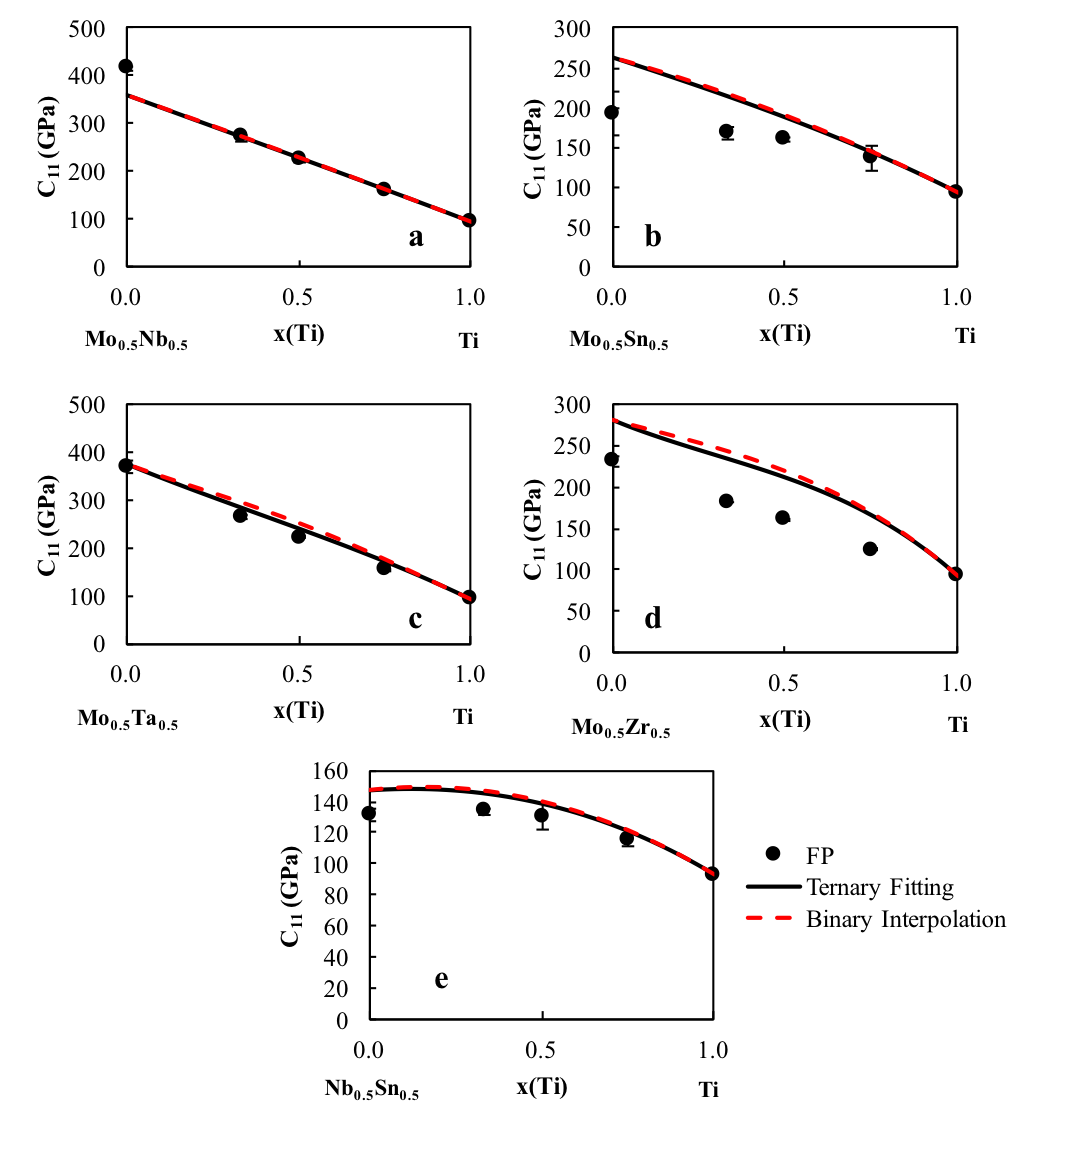
\includegraphics[width=\textwidth]{Chapter-6/Figures/tixyc111.png}
	\caption{Calculated $\overline{C}_{11}$ values (circles) plotted with their errors as well as the interpolation from the binary interaction parameters (red dashed line) and the ternary fitting (black dashed line) for five of the Ti-X-Y binary systems from a 50-50 mixture of the alloying elements X and Y to Ti (X $\neq$ Y = Mo, Nb, Ta, Sn, Zr).}
	\label{Ch6-figure:tixyc11_1}
\end{figure}

\pagebreak
\begin{figure}[H]
	\centering
	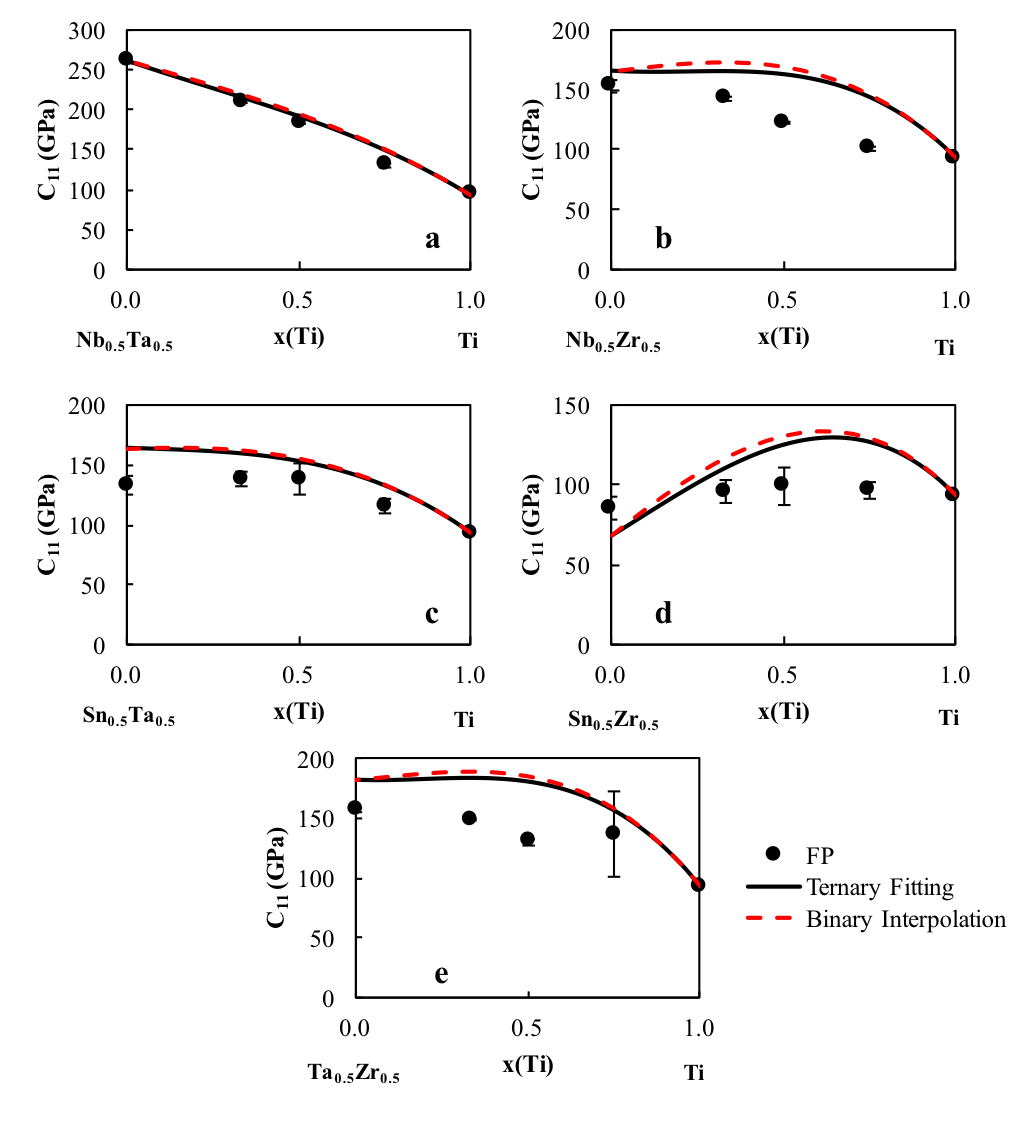
\includegraphics[width=\textwidth]{Chapter-6/Figures/tixyc112.png}
	\caption{Calculated $\overline{C}_{11}$ values (circles) plotted with their errors as well as the interpolation from the binary interaction parameters (red dashed line) and the ternary fitting (black dashed line) for five of the Ti-X-Y binary systems from a 50-50 mixture of the alloying elements X and Y to Ti (X $\neq$ Y = Mo, Nb, Ta, Sn, Zr).}
	\label{Ch6-figure:tixyc11_2}
\end{figure}


\pagebreak
\begin{figure}[H]
	\centering
	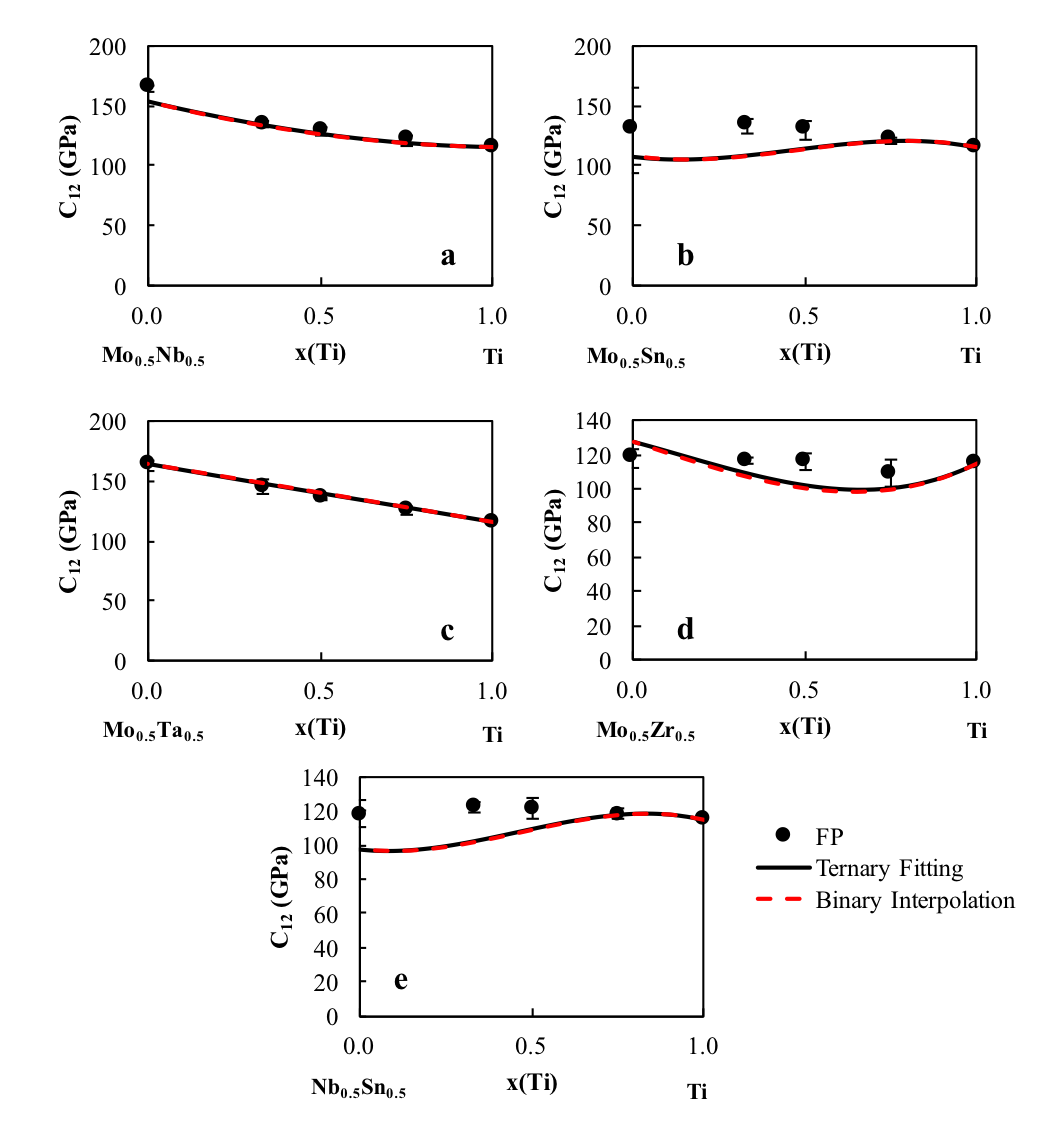
\includegraphics[width=\textwidth]{Chapter-6/Figures/tixyc121.png}
	\caption{Calculated $\overline{C}_{12}$ values (circles) plotted with their errors as well as the interpolation from the binary interaction parameters (red dashed line) and the ternary fitting (black dashed line) for five of the Ti-X-Y binary systems from a 50-50 mixture of the alloying elements X and Y to Ti (X $\neq$ Y = Mo, Nb, Ta, Sn, Zr).}
	\label{Ch6-figure:tixyc12_1}
\end{figure}

\pagebreak
\begin{figure}[H]
	\centering
	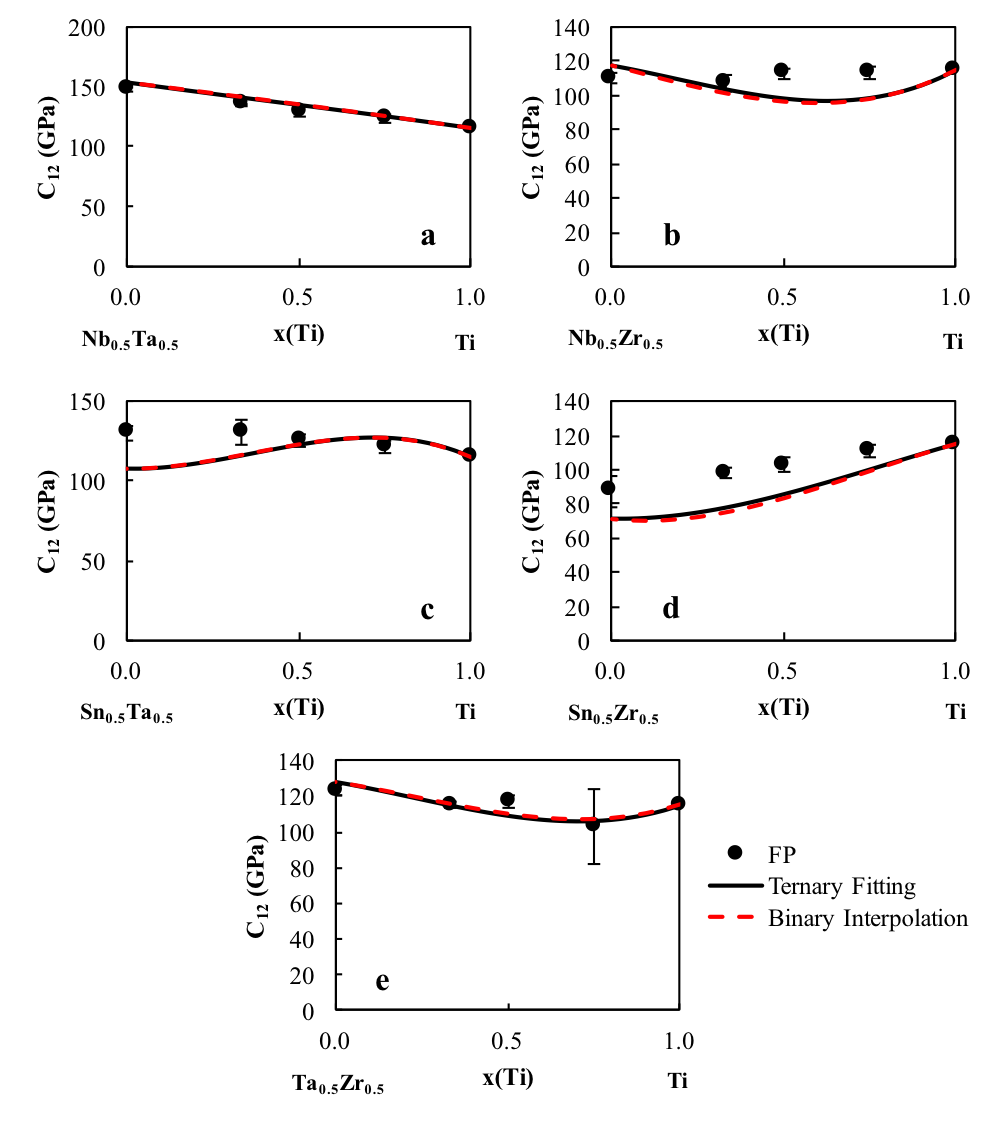
\includegraphics[width=\textwidth]{Chapter-6/Figures/tixyc122.png}
	\caption{Calculated $\overline{C}_{12}$ values (circles) plotted with their errors as well as the interpolation from the binary interaction parameters (red dashed line) and the ternary fitting (black dashed line) for five of the Ti-X-Y binary systems from a 50-50 mixture of the alloying elements X and Y to Ti (X $\neq$ Y = Mo, Nb, Ta, Sn, Zr).}
	\label{Ch6-figure:tixyc12_2}
\end{figure}

\pagebreak
\begin{figure}[H]
	\centering
	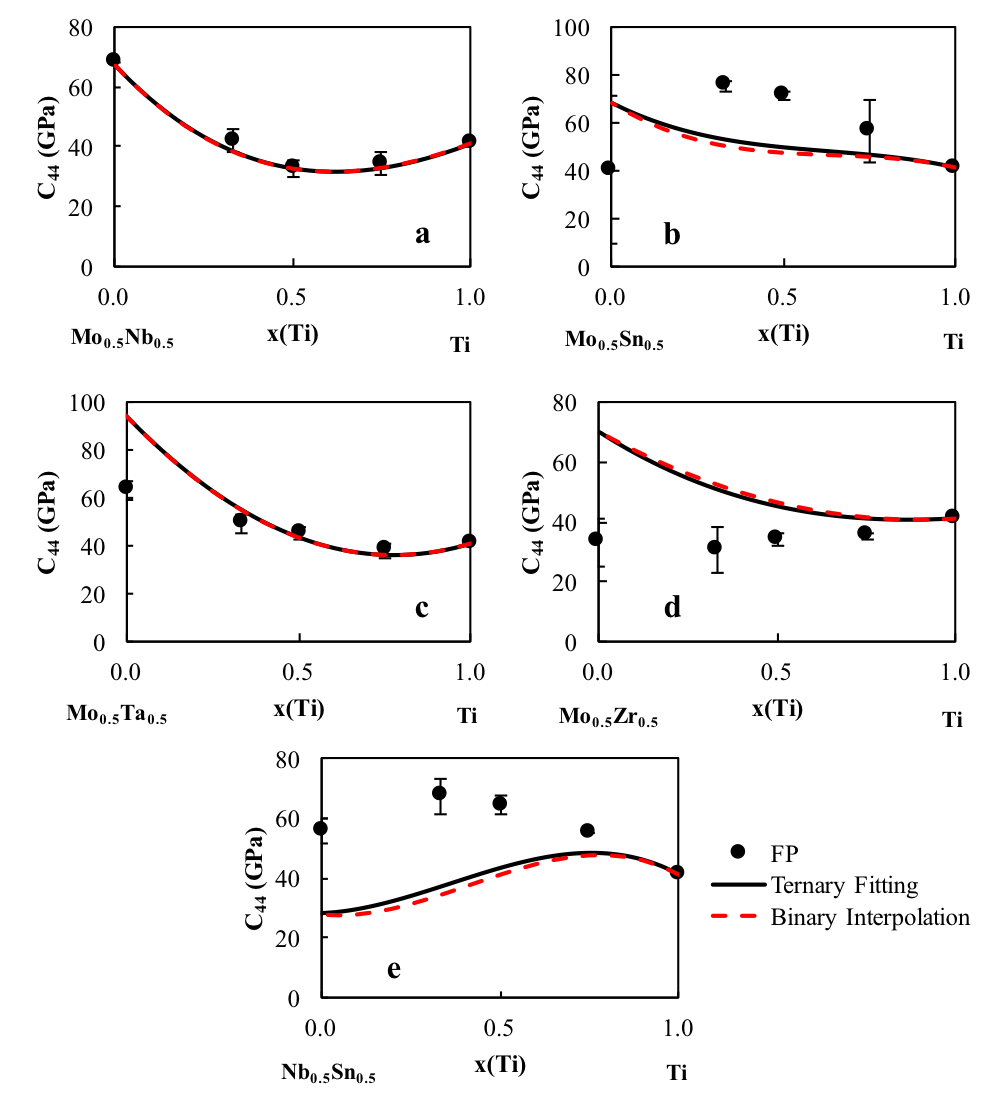
\includegraphics[width=\textwidth]{Chapter-6/Figures/tixyc441.png}
	\caption{Calculated $\overline{C}_{44}$ values (circles) plotted with their errors as well as the interpolation from the binary interaction parameters (red dashed line) and the ternary fitting (black dashed line) for five of the Ti-X-Y binary systems from a 50-50 mixture of the alloying elements X and Y to Ti (X $\neq$ Y = Mo, Nb, Ta, Sn, Zr).}
	\label{Ch6-figure:tixyc44_1}
\end{figure}

\pagebreak
\begin{figure}[H]
	\centering
	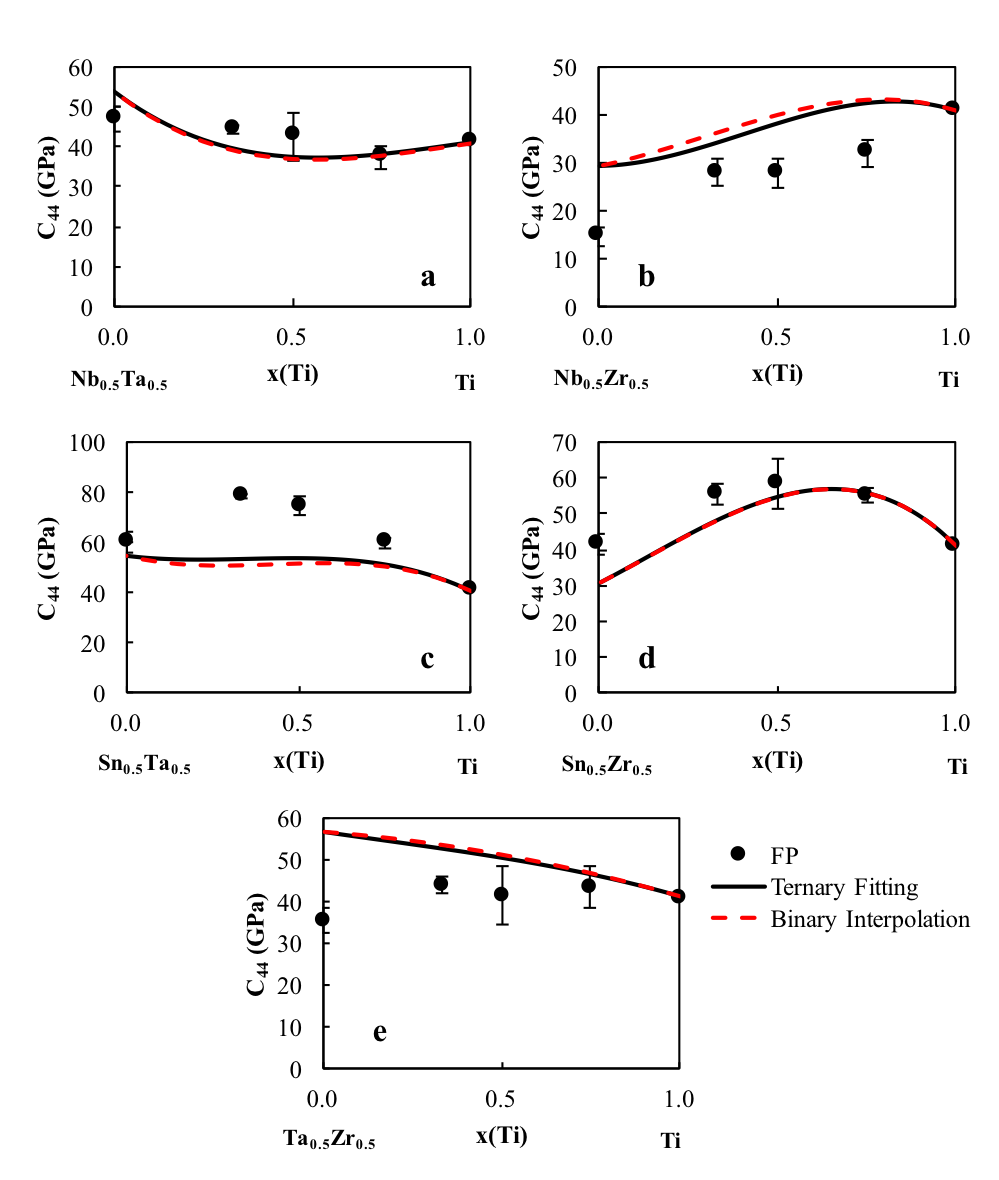
\includegraphics[width=\textwidth]{Chapter-6/Figures/tixyc442.png}
	\caption{Calculated $\overline{C}_{44}$ values (circles) plotted with their errors as well as the interpolation from the binary interaction parameters (red dashed line) and the ternary fitting (black dashed line) for five of the Ti-X-Y binary systems from a 50-50 mixture of the alloying elements X and Y to Ti (X $\neq$ Y = Mo, Nb, Ta, Sn, Zr).}
	\label{Ch6-figure:tixyc44_2}
\end{figure}

\pagebreak
\begin{figure}[H]
	\centering
	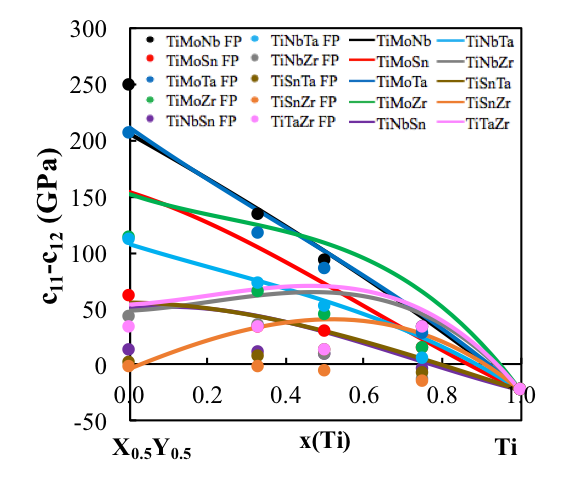
\includegraphics[width=\textwidth]{Chapter-6/Figures/tixyc11-c12.png}
	\caption{Calculated $\overline{C}_{11}$-$\overline{C}_{12}$ values (circles) plotted with the present modeling (solid lines) for the Ti-X-Y ternary systems (X $\neq$ Y = Mo, Nb, Ta, Sn, Zr). The $\overline{C}_{11}$-$\overline{C}_{12}$ shows the stability of the bcc phase, when the value is negative the bcc phase is not stable in the corresponding composition ranges.}
	\label{Ch6-figure:tixyc11-c12}
\end{figure}

\pagebreak
\begin{figure}[H]
	\centering
	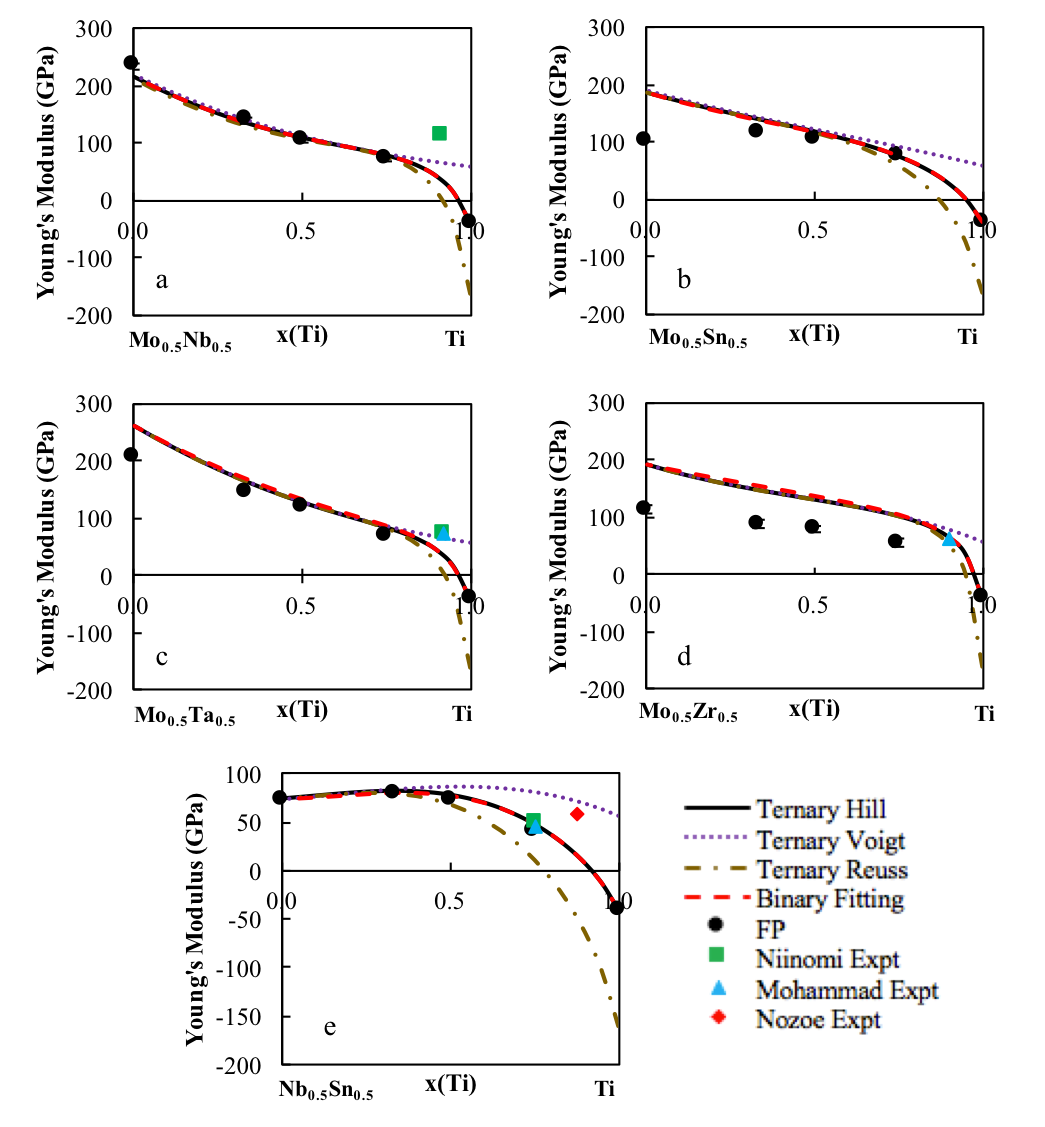
\includegraphics[width=\textwidth]{Chapter-6/Figures/tixyyoungs1.png}
	\caption{$E$ of five of the Ti-X-Y ternary systems are plotted from a 50-50 mixture of the alloying elements to Ti in the bcc phase. The present calculations are plotted as filled circles with the error bars. The red dotted line is the extrapolation for the pure elements and binary interaction parameters only. The dotted purple line is the Voigt upper $E$ bound, the gold dot dashed line is the lower Reuss $E$ bound and the black line is the Hill $E$ average. Experimental values are include for comparison \cite{Niinomi2012,Mohammed2014,Nozoe2007,Geetha2009}.}
	\label{Ch6-figure:tixyyoungs1}
\end{figure}

\pagebreak
\begin{figure}[H]
	\centering
	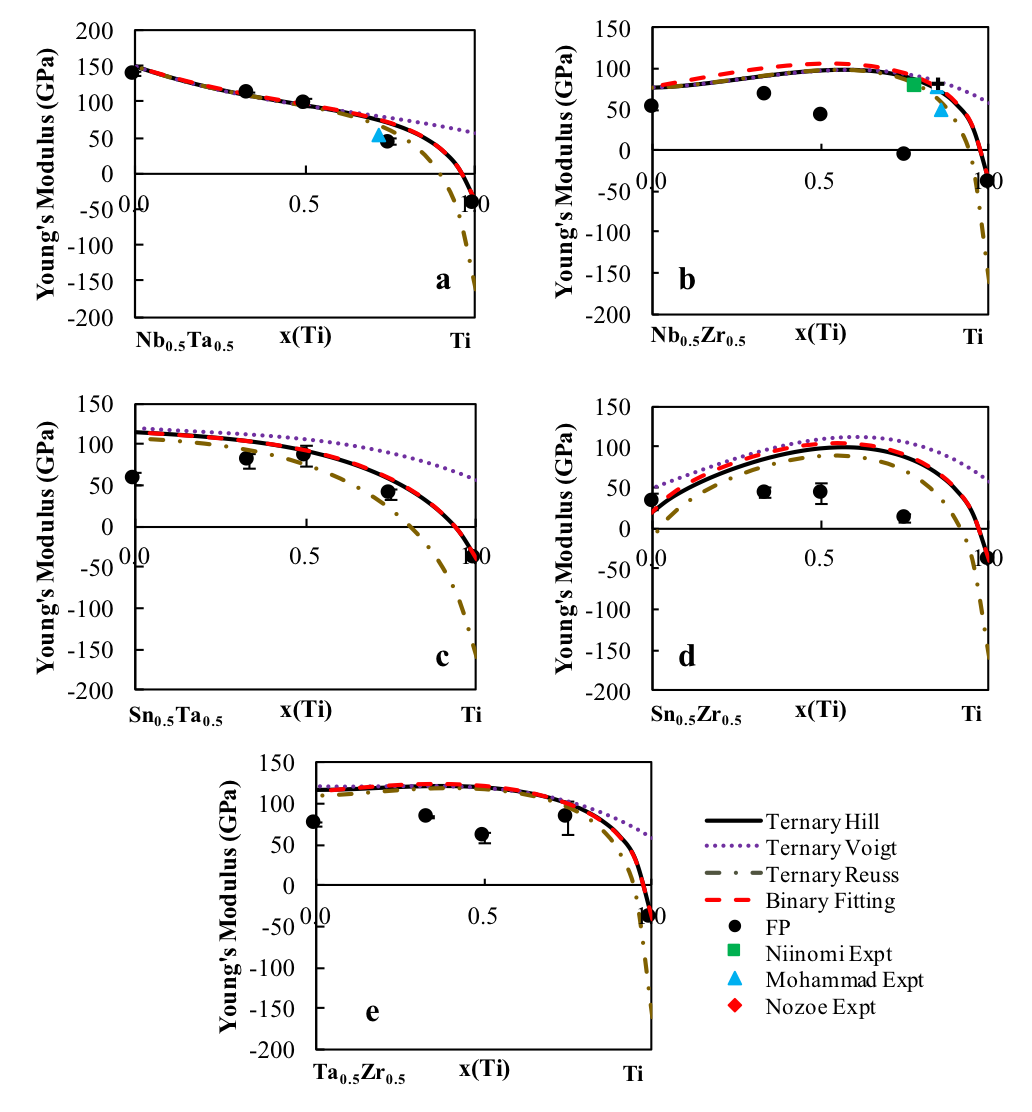
\includegraphics[width=\textwidth]{Chapter-6/Figures/tixyyoungs2.png}
	\caption{$E$ of five of the Ti-X-Y ternary systems are plotted from a 50-50 mixture of the alloying elements to Ti in the bcc phase. The present calculations are plotted as filled circles with the error bars. The red dotted line is the extrapolation for the pure elements and binary interaction parameters only. The dotted purple line is the Voigt upper $E$ bound, the gold dot dashed line is the lower Reuss $E$ bound and the black line is the Hill $E$ average. Experimental values are include for comparison \cite{Niinomi2012,Mohammed2014,Nozoe2007,Geetha2009}.}
	\label{Ch6-figure:tixyyoungs2}
\end{figure}

\pagebreak
\begin{figure}[H]
	\centering
	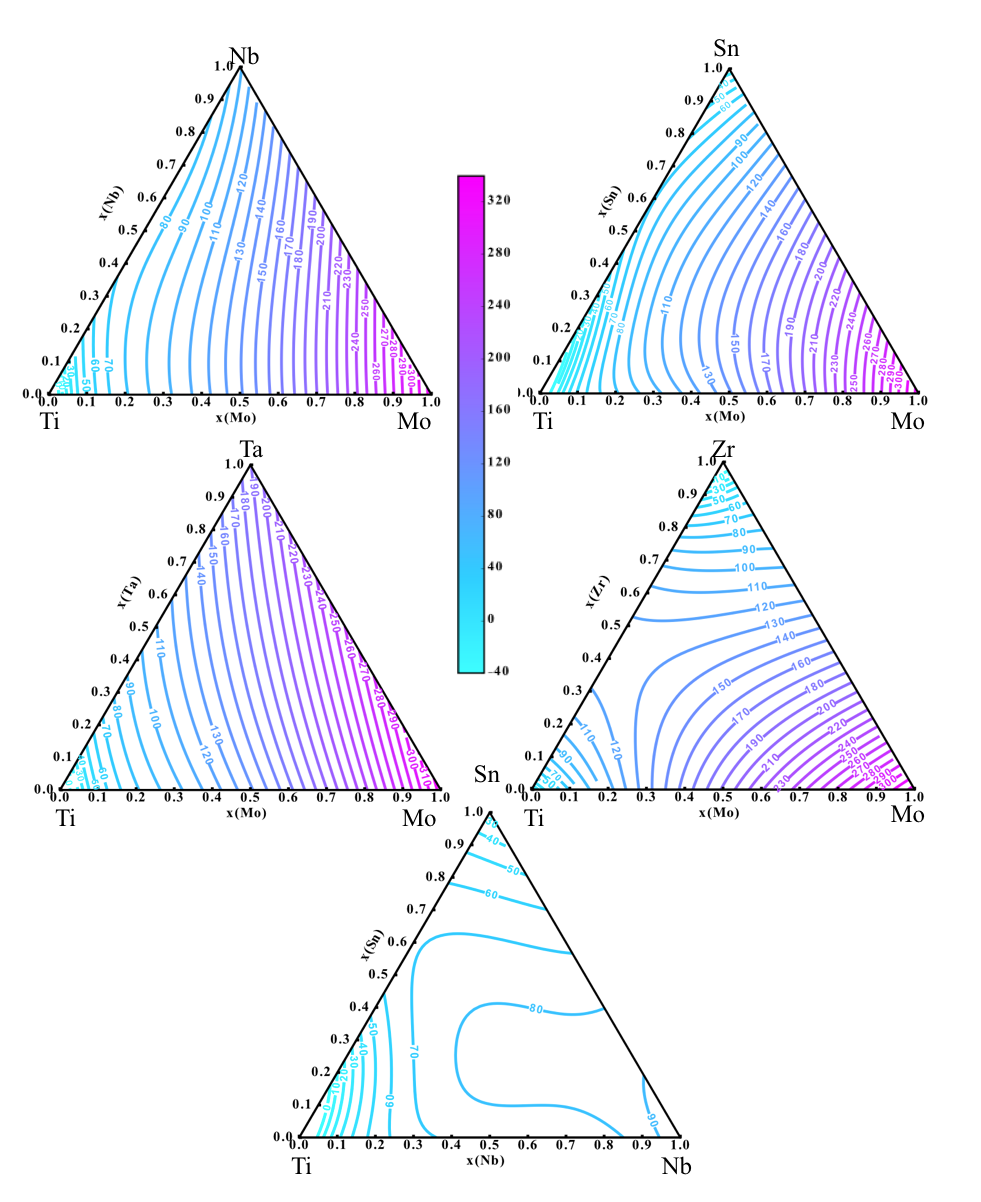
\includegraphics[width=\textwidth]{Chapter-6/Figures/tixymap1.png}
	\caption{The Young's modulus is mapped as a function of composition in GPa for the Ti-Mo-Nb, Ti-Mo-Sn, Ti-Mo-Ta, Ti-Mo-Zr and Ti-Nb-Sn alloy systems using pycalphad \cite{Otis2017}.}
	\label{Ch6-figure:tixymap1}
\end{figure}

\pagebreak
\begin{figure}[H]
	\centering
	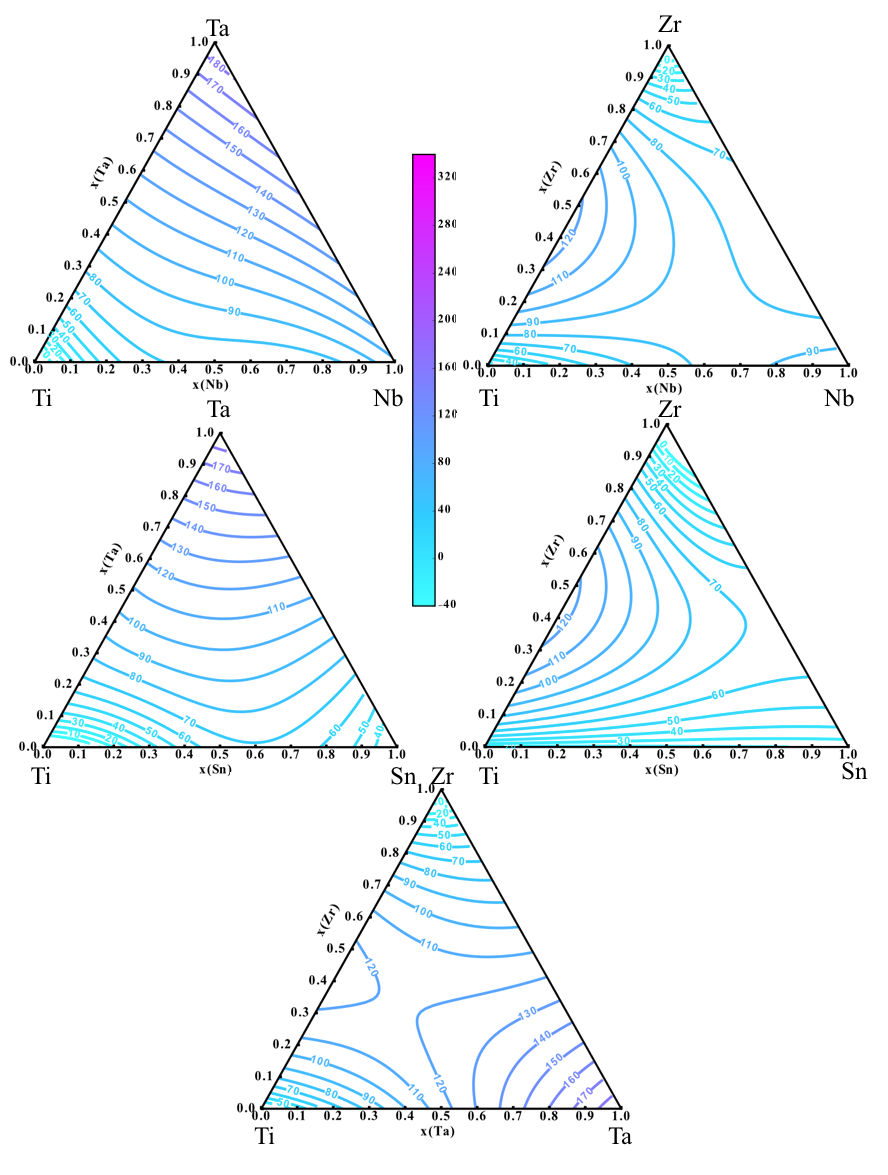
\includegraphics[width=\textwidth]{Chapter-6/Figures/tixymap2.png}
	\caption{The Young's modulus is mapped as a function of composition in GPa for the Ti-Mo-Nb, Ti-Mo-Sn, Ti-Mo-Ta, Ti-Mo-Zr and Ti-Nb-Sn alloy systems using pycalphad \cite{Otis2017}.}
	\label{Ch6-figure:tixymap2}
\end{figure}

\pagebreak
\begin{figure}[H]
	\centering
	\includegraphics[width=\textwidth]{Chapter-6/Figures/tixybulk1.png}
	\caption{$B$ calculations of five of the Ti-X-Y ternary systems (X $\neq$ Y = Mo, Nb, Ta, Sn, Zr). The present calculations are plotted as the filled circles with error bars as well as the interpolation from the binary interaction parameters (red dashed line). The dotted purple line is the Voigt upper bulk modulus bound, the gold dashed line is the lower Reuss bulk modulus bound and the black line is the Hill bulk modulus average plotted from a 50-50 mixture of the alloying elements X and Y to Ti.}
	\label{Ch6-figure:tixybulk1}
\end{figure}

\pagebreak
\begin{figure}[H]
	\centering
	\includegraphics[width=\textwidth]{Chapter-6/Figures/tixybulk2.png}
	\caption{$B$ calculations of five of the Ti-X-Y ternary systems (X $\neq$ Y = Mo, Nb, Ta, Sn, Zr). The present calculations are plotted as the filled circles with error bars as well as the interpolation from the binary interaction parameters (red dashed line). The dotted purple line is the Voigt upper bulk modulus bound, the gold dashed line is the lower Reuss bulk modulus bound and the black line is the Hill bulk modulus average plotted from a 50-50 mixture of the alloying elements X and Y to Ti.}
	\label{Ch6-figure:tixybulk2}
\end{figure}

\pagebreak
\begin{figure}[H]
	\centering
	\includegraphics[width=\textwidth]{Chapter-6/Figures/tixyshear1.png}
	\caption{$G$ calculations of five of the Ti-X-Y ternary systems (X $\neq$ Y = Mo, Nb, Ta, Sn, Zr). The present calculations are plotted as the filled circles with error bars as well as the interpolation from the binary interaction parameters (red dashed line). The dotted purple line is the Voigt upper shear modulus bound, the gold dashed line is the lower Reuss shear modulus bound and the black line is the Hill shear modulus average plotted from a 50-50 mixture of the alloying elements X and Y to Ti.}
	\label{Ch6-figure:tixyshear1}
\end{figure}

\pagebreak
\begin{figure}[H]
	\centering
	\includegraphics[width=\textwidth]{Chapter-6/Figures/tixyshear2.png}
	\caption{$G$ calculations of five of the Ti-X-Y ternary systems (X $\neq$ Y = Mo, Nb, Ta, Sn, Zr). The present calculations are plotted as the filled circles with error bars as well as the interpolation from the binary interaction parameters (red dashed line). The dotted purple line is the Voigt upper shear modulus bound, the gold dashed line is the lower Reuss shear modulus bound and the black line is the Hill shear modulus average plotted from a 50-50 mixture of the alloying elements X and Y to Ti.}
	\label{Ch6-figure:tixyshear2}
\end{figure}

\pagebreak
\begin{figure}[H]
	\centering
	\includegraphics{Chapter-6/Figures/tixydatabase.png}
	\caption{$E$ of multicomponent bcc Ti alloys predicted from the database are compared with measured experimental results. Error bars plotted are from the variation in experimentally determined Young's moduli values for the specific multi-component alloy. The grey region refers to the error in the first-principles calculations. More information on the alloys is Table \ref{Ch6-table:tixydatacomp} \cite{Mohammed2014,Geetha2009,Tane2010a}.}
	\label{Ch6-figure:tixydatabase}
\end{figure}
\chapter{Metastable phase study in the Ti-Ta and Ti-Nb systems}

\section{Introduction}

The present chapter is aimed at studying the formation of the metastable phases $\omega$ and $\alpha"$. As shown in Figures \ref{Ch1-figure:titaelastic} and \ref{Ch1-figure:tinbelasitc}, the formation of the $\alpha"$ and $\omega$ phases affects the elastic properties of Ti-Ta and Ti-Nb alloys. Currently the CALPHAD method predicts the equilibrium phase formation. For Ti-Nb, the CALPHAD method predicts that the alloys will form either the single hcp or bcc phases or a two-phase mixture of bcc and hcp. Understanding the effect of the metastable phases on the elastic properties and being able to predict at what compositions they form, will help with alloy selection and increase the likelihood of finding a suitable alloy for load-bearing implants. The stability of the bcc, hcp, $\omega$, and $\alpha"$ phases at 0 K is calculated and discussed for the Ti-Ta and Ti-Nb alloys using multiple structures across the entire composition range. The elastic properties of the four phases are then calculated systematically and interaction parameters are introduced using the CALPHAD method, similar as described in chapter 5, to be able to predict the elastic properties as a function of composition. With an understanding of how the phases affect the elastic properties, an adaptation of the partition function approach, was introduced (in chapter 2) to be able to predict the formation of the metastable phases. In order to ensure the accuracy of the theoretic framework, neutron scattering experiments are completed on 4 different Ti-Nb compositions. The data from the experiments is used to determine the phase fractions and phonon density of states. The results from the neutron scattering are compared with the theoretical results. The determined phase fractions are used to predict the elastic properties and compared with experimental values in the literature.

\section{Modeling and Calculations}

\subsection{Computational details}

In the present work, the Vienna ab-initio Simulation Package (VASP) \cite{Kresse1996} was employed to calculate the ground state energy and elastic properties of the pure elements and Ti-Nb and Ti-Ta systems in the bcc, hcp, $\omega$, and $\alpha"$ phases. The ion-electron interactions were described using the projector augmented wave (PAW) \cite{Kresse1999,Blochl1994} method and based on the previous work of comparing X-C functionals (Figure \ref{Ch5-figure:PBEvsPW91}) the exchange-correlation functional of the generalized gradient approach depicted by Perdew, Burke, and Ernzerhof (PBE-GGA) was employed \cite{Perdew1996a}. The energy convergence criterion of the electronic self-consistency was set as 10$^{-6}$ eV/atom. Indepedent structures based on the ATAT code were generated for the four phases, bcc (330), hcp (21), $\alpha"$ (33) and $\omega$ (73), across the entire composition range. The Brillouin zone sampling was done using the $\Gamma$-centered Monkhorst-Pack scheme \cite{Monkhorst1976a}. The k-points grid for the hcp, $\omega$ and $\alpha"$ phases were 10x10x13, 13x13x7, and 12x11x10, respectively. The k-point grids fro the bcc calculations used the automated k-point mesh generator in VASP with the length of the subdivisions specificed as 50. The elastic properties were then calculated using a $\pm$0.01 magnitude of strain.

\subsection{Modeling details}

The elastic stiffness coefficients were modeled using the first-principles based DFT results. The modeling was completed by the methodology outlined in chapter 2. The difference between the first-principles calculations and the linear combination from the pure elements was caculated and the fittings were completed and the interaction parameters were fit using the code in appendix C. The best fit was found by comparing the fittings obtained with one interaction parameter or with two interaction parameters. The moduli values were than calculated using pycalphad and the code in appendix D and E \cite{Otis2017}.

\section{Results and discussion}

\subsection{First-principles calculations at 0 K}

The phase stability at 0 K is calculated as a function of composition for the Ti-Nb and Ti-Ta systems. Figure \ref{Ch7-figure:tinb0K} and \ref{Ch7-figure:titab0K} show the relative energy of the bcc, hcp, $\omega$, and $\alpha"$ phases from 100 at. \% Ti to 100 at. \% Nb or Ta. The relative energies are calculated according to Eq. \ref{eq: hform} using the ground state energies of the pure elements in the SER state as reference. Figure \ref{Ch7-figure:titab0K} is the relative energy of the bcc, hcp, $\omega$, and $\alpha"$ phases from 100 at. \% Ti to 100 at. \% Ta. Figure \ref{Ch7-figure:tinb0K} and \ref{Ch7-figure:titab0K} are both at 0 K. The calculations are still ongoing for Figure \ref{Ch7-figure:tinb0K}. The figures show that the relative energy of the hcp phase starts negative and then increases to pure Nb or Ta. The bcc phase starts with a higher relative energy at pure Ti and then decreases to negative at pure Nb or Ta. The hcp phase is lower relative energy to 30 at. \% Nb when the bcc phase has a lower relative energy. The $\omega$ and $\alpha"$ have similar relative energies at pure Ti and some of the structures continue to have similar relative energies from pure Ti to 80 at. \% Nb or Ta.

Kim et al.  \cite{Kim2006} figured out the martensitic transformation temperature for Ti-Nb alloys between 20 and 30 at. \% Nb, shown in Figure \ref{Ch7-figure:titnbms}. Based on this available information, the Ti-Nb system is studied more in depth in the remaining parts of this chapter. 

\subsection{Elastic properties}

For the Ti-Nb system, the elastic stiffness coefficients of the bcc, hcp, $\alpha"$, and $\omega$ phases are calculated. The calculations and interaction parameters of the bcc phase are discussed in chapter 5. Figure \ref{Ch7-figure:adpelas1} and \ref{Ch7-figure:adpelas2} plot the elastic stiffness coefficients, $c_{11}$, $c_{12}$, $c_{13}$, $c_{22}$, $c_{23}$, $c_{33}$, $c_{44}$, $c_{55}$, and $c_{66}$, for the $\alpha"$ phase. The plots show the first-principles results (circles), the linear combination from the pure elements (dashed red line) and the fitting (solid line) using the interaction parameters in Table \ref{Ch7-table:intpara}. The $c_{11}$ and $c_{22}$ values decrease from 198 GPa and 197 GPa to 140 GPa and 152 GPa at 25 at. \% Nb then increase to 307 GPa and 242 GPa at 95 at. \% Nb and finally decrease to 306 GPa and 240 GPa at pure Nb, respectively. The $c_{12}$ values increase from 69 GPa at 0 at. \% Nb to 120 GPa at 40 at. \% Nb and then decrease to 88 GPa pure Nb. The $c_{13}$ values increase from 84 GPa at 0 at. \% Nb to 125 GPa 30 at. \% Nb, then decrease to 101 GPa 80 at. \% Nb and then increase to 125 GPa at pure Nb. The $c_{23}$ values decrease from 84 GPa at 0 at. \% Nb to 53 GPa at 25 at. \% Nb and then increase to 135 GPa at pure Nb. The $c_{33}$ values decrease from 189 GPa at pure Ti to 99 GPa at 50 at. \% Nb and then increase to 284 GPa at pure Nb. The $c_{44}$ values increase from 40 GPa at pure Ti to 47 GPa at pure Nb. The $c_{55}$ values decrease from 40 GPa at pure Ti to 4 GPa at 20 at. \% Nb, then increase to 41 GPa at 65 at. \% Nb and then decrease to -69 GPa at pure Nb. The $c_{66}$ decreases in value from 63 GPa at pure Ti to 13 GPa at 60 at. \% Nb then increases to 14 GPa at 85 at. \% Nb and then decrease to 9 GPa at pure Nb.

Figure \ref{Ch7-figure:omegae1} plots the elastic stiffness coefficients, $c_{11}$, $c_{12}$, $c_{13}$, $c_{33}$, and $c_{44}$, for the $\omega$ phase. The plots show the first-principles results (circles), the linear combination from the pure elements (dashed red line) and the fitting (solid line) using the interaction parameters in Table \ref{Ch7-table:intpara}. The $c_{11}$ values decrease from 194 at pure Ti to 164 GPa at 25 at. \% Nb and then increase to 243 at pure Nb. The $c_{12}$ values increase from 87 at pure Ti to 94 GPa at 10 at. \% Nb, then decrease to -129 at 65 at. \% Nb and then increase to 181 at pure Nb. The $c_{13}$ values increase from 61 GPa at pure Ti to 189 GPa at 70 at. \% Nb and then decrease to 110 at pure Nb. The $c_{33}$ values decrease from 246 GPa at pure Ti to 152 GPa at 25 at. \% Nb, then increase to 283 GPa at 80 at. \% Nb and then decrease to 212 GPa at pure Nb. The $c_{44}$ values decrease from 54 GPa at pure Ti to 29 GPa at 20 at. \% Nb, then increase (in value) to 74 GPa at 70 at. \% Nb and then decrease to -55 GPa at pure Nb.

Figure \ref{Ch7-figure:hcpe1} plots the elastic stiffness coefficients, $c_{11}$, $c_{12}$, $c_{13}$, $c_{33}$, and $c_{44}$, for the hcp phase. The plots show the first-principles results (circles), the linear combination from the pure elements (dashed red line) and the fitting (solid line) using the interaction parameters in Table \ref{Ch7-table:intpara}.The $c_{11}$ values increase from 175 GPa at pure Ti to 190 GPa at 10 at. \% Nb and then decrease to 56 GPa at 70 at. \% Nb and then increase to 165 at pure Nb. The $c_{12}$ values decrease from 88 GPa at pure Ti to 83 GPa at 10 at. \% Nb and then increase to 237 GPa at pure Nb. The $c_{13}$ values decrease from 80 GPa at pure Ti to 78 GPa at 10 at. \% Nb, then increase from to 154 GPa at 75 at. \% Nb and then decrease (in value) to 111 GPa at pure Nb. The $c_{33}$ values decrease from 190 GPa at pure Ti to 179 GPa at 45 at. \% Nb, then increase to 241 GPa at pure Nb. The $c_{44}$ values decrease from 41 GPa at pure Ti to -66 GPa at 95 at.\% Nb, then increase to -65 GPa at pure Nb.

The interaction parameters determined are listed in \ref{Ch7-table:intpara} and the calculated elastic stiffness coefficients and $E$ values are listed in Table \ref{Ch7-table:tinbdata}. The Young's moduli values are calculated as a function of composition and are plotted in Figure \ref{Ch7-figure:tinbelastic}. The dotted lines are the fittings that use the interaction parameters in Table \ref{Ch7-table:intpara}. The calculations show that the Young's moduli for the hcp phase decrease (in value) from pure Ti (124 GPa) until 60 at. \% Nb (-78 GPa) and then increase from 80 at. \% Nb to pure Nb (15 GPa). The Young's moduli, for the $\omega$ phase, follows the same trend as the hcp phase. The $E$ values decrease from pure Ti (152 GPa) to around pure Nb (-158 GPa). The $E$ values for the bcc phase increase from -40 GPa at pure Ti to 98 GPa at pure Nb. The $E$ values for the $\alpha"$ phase decrease from 133 GPa at pure Ti to 94 GPa at 20 at. \% Nb, then increase to 138 GPa 70 at. \% Nb and then decrease to 97 GPa at pure Nb. The $E$ values for the hcp, $\omega$, and bcc phases all become negative at certain compositions. Based on Born's criteria, a negative Young's modulus can indicate that the phase is not stable at that composition. From Figure \ref{Ch7-figure:tinbelastic} it can be seen that the $E$ values of the $\alpha"$ phase are higher than the $E$ values of the hcp or bcc phases. This explains why the experimental Young's moduli increase in value with the formation of $\alpha$, as seen in Figure \ref{Ch1-figure:tinbelasitc}. 

Different authors experimentally determined the $E$ of various Ti-Nb alloys at different compositions, as seen in Figure \ref{Ch1-figure:tinbelasitc}, \cite{Friak2012,Timoshevskii2011,Friak2012,Karre2015}. Ozaki et al. \cite{Ozaki2004} showed that at certain compositions quenched Ti-Nb samples formed bcc and $\alpha"$ while the slow cooled samples formed bcc and $\omega$, which is in agreement with this work. For the quenched samples, there is more data available in the literature \cite{Friak2012,Timoshevskii2011,Friak2012,Karre2015}, and therefore the present work averaged the $E$ values obtained by different researchers for the same compositions. A full review of the experimental results are listed in appendix F and the averaged experimental values are listed in Table \ref{Ch7-table:elasexptdata}. From these experiments, some of the phase fractions were determined \cite{Friak2012} and those phase fractions are listed in Table \ref{Ch7-table:elasexptdata}. For the compositions where the phase fractions were not determined, we extrapolated an estimated phase fractions at each composition. Those estimated phase fractions are differentiated from the experimentally determined phase fractions by labeling them with a *. Then, the rule of mixtures was used as a beginning estimate of the Young's moduli values based on these phase fractions and the interaction parameters in Table \ref{Ch7-table:intpara}. The rule of mixtures is expressed by:

%%
\begin{equation}
\label{eq:ruleofmix}
E_{c}=x_{p1}E_{p1}+x_{p2}E_{p2}
\end{equation}
%%

\noindent where $x_{p1}$ and $x_{p2}$ are the phase fractions of phase 1 and phase 2, respectively and $E_{p1}$ and $E_{p2}$ are the $E$ in phase 1 and phase 2, respectively. Based on the observations in literature \cite{Friak2012,Timoshevskii2011,Friak2012,Karre2015}, from pure Ti to 10 at. \% Nb the samples are 100 \% hcp and the predicted $E$ vary, on average, from the experimental $E$ by 3 GPa. From 10 at. \% Nb to 30 at. \% Nb, the hcp phase formation is repressed and the $\alpha"$ and bcc phases formed. The exact phase fraction of the bcc phase was measured by Friak et al. \cite{Friak2012} for samples with 10, 20, 25, and 30 at. \% Nb. An extrapolation from these values is used to estimate the phase fractions of the remaining alloy compositions, in this composition range. Using the phase fractions and rule of mixtures, the predicted $E$ vary, on average, from the experimental $E$ by 0.52 GPa. This is significantly more accurate than the 22 GPa error between the experimental and predicted $E$ using the bcc and hcp mixture predicted by CALPHAD. Above 33 at. \% Nb the samples consist of the single bcc phase. The predicted $E$ vary, on average, by 7 GPa from the experimental $E$ by 7 GPa. Overall, the variances are small when compared to the variances in the experiments. As seen in appendix F, the experimental $E$ values of pure Ti in the hcp phase vary by 24 GPa. The variance between the predicted $E$ and experimental $E$ can be attributed to the fact that the predicted $E$ are at 0 K and the experimental $E$ are measured at 300 K. It is evident that the database can be used with the rule of mixtures to accurately predict the elastic properties of Ti-Nb alloys if the phase fraction of the metastable phases can be predicted.

\subsection{Neutron scattering results}

\subsubsection{Phonon density of states at 300 K}

In order to predict when the metastable phases form, four Ti-Nb alloys were measured using the ARCS neutron scattering instrument at the Spallation Neutron Source, Oak Ridge National Laboratory. As discussed in the methodology, two sets of samples were made. Each set contains a Ti-Nb alloy at the following compositions: 10, 12, 18, 20 at. \% Nb. The two sets of samples were annealed at 1273 K for 24 hours. One set of samples was quenched in cold water to form the bcc and $\alpha"$ phases while the second set of samples was slow cooled to form the bcc and $\omega$ phases. Neutron scattering was then done at 300 K

In Figure \ref{Ch7-figure:50dos20}, \ref{Ch7-figure:50dos18}, \ref{Ch7-figure:50dos12}, \ref{Ch7-figure:50dos10} the phonon density of states (DOS) at 300 K is plotted for each sample. The samples at the same compositions are plotted in on figure for comparison. The phonon DOS of the slow cooled samples are plotted as dashed lines and the phonon DOS of the quenched samples are plotted as solid lines. It can be seen that the quenched samples show different phonon DOS than the slow cooled samples, which means that the samples have different phases. In order to investigate the difference of the phonon DOS further the entropy of each sample is calculated from the phonon DOS ($g(E)$):

%%
\begin{equation}
\label{eq:phononentropy}
S_{vib} = 3 k_{B} \int_{0}^{E_{max}} \left[ \left( n+1 \right) ln\left(n+1\right) -n ln\left(n\right) \right] g(E) dE
\end{equation}
%%

\noindent where $n$ is the Bose-Einstein occupation factor \cite{Budai2014}. The entropy difference between the alloys at the same compositions is plotted in \ref{Ch7-figure:ediff}. The figure shows that the entropy difference is less than 0.02 kB/atom between the two 10 at. \% Nb samples. The entropy difference then increases to less than 0.03 between the two 12 at. \% Nb samples and less than 0.06 between the two 18 at. \% Nb samples. Finally, the entropy difference between the two 20 at. \% Nb samples reaches a peak close to 0.1 kB/atom This would result in a 30 kB/atom free energy difference between the samples. Further investigations on these samples are necessary to understand and explain this observation.

\subsubsection{Diffraction patterns at 300 K}

The diffraction patterns for each alloy are plotted in Figure \ref{Ch7-figure:50diff20}, \ref{Ch7-figure:50diff18}, \ref{Ch7-figure:50diff12}, and \ref{Ch7-figure:50diff10}. The slow cooled samples are plotted as solid lines and the quenched samples are plotted as dashed lines. The diffraction patterns plot the intensity vs. momenta (Q). The plots are compared with diffraction patterns of Ti and Nb in the four phases from the literature to determine an approximation of the phase fractions, which are listed in Table \ref{Ch7-table:phasefrac}. It can be seen that the phase fractions of the bcc phase of the quenched samples are 0.12, 0.20, 0.57 and 0.70 for the samples containing 10, 12, 18 and 20 at. \% Nb, respectively. The slow cooled samples showed  a phase fraction of the bcc phase of 0.2, 0.3, 0.6, and 0.7 for the samples containing 10, 12, 18, and 20 at. \% Nb, respectively. The phase fractions of the quenched samples with 10 and 20 at. \% Nb compare well with the fractions determined by Friak et al. \cite{Friak2012}, as shown in Table \ref{Ch7-table:elasexptdata}. 

To further understand the phase formation in Ti-Nb alloys the temperature dependence of these alloys will be studied by neutron scattering experiments at 500, 900 and 1110 K. Additionally, x-ray diffraction (XRD) will be conducted on the samples. The temperature dependence of the phonon DOS will provide information about the type of transformation taking place, while XRD will provide more detailed information about the phase fractions in the samples.

\subsection{Partition function approach results}

The implementation of the new theoretical framework is in progress. To get started, the combined Helmholtz energy, Eq. \ref{eq: combinedhelmholtz}, of pure Ti in the hcp, bcc, $\omega$ and $\alpha"$ phases was calculated, since the energy term representing composition can be ignored for these calculations. The ground state energy at 0 K is mapped for Ti in the four phases and the energy minima is identified. Quasiharmonic phonon calculations will be completed on the structures at the lowest energy minima points. The Helmholtz energy results and eigenvalues from these calculations will be used in Eq. \ref{eq: combinedhelmholtz}, \ref{eq: combinedhelmholtz2}, \ref{eq: zc}, and \ref{eq: zi}. Using the calculation of entropy from the combined Helmholtz this work should more accurately predict the Helmholtz energy of Ti in the four phases. Once the work has finished for pure Ti, the partition function approach will be extended to account for the change in composition in the Ti-Nb binary system and compared to the neutron scattering results. With the combined Helmholtz energy, the phonon density of states and phase fractions predicted should agree with the phonon DOS and phase fractions obtained from the neutron scattering.

\section{Conclusion}

The present study systematically calculated the elastic stiffness coefficients and Young's moduli of the Ti-Nb system in the bcc, hcp, $\omega$, and $\alpha"$ phases. The general CALPHAD modeling approach was used to fit binary interaction parameters. The $E$ values were similar for the hcp and $\omega$ phase, which is reasonable since they both have hexagonal symmetry. The $\alpha"$ phase has $E$ values that were higher than the other three phases which explains why the $E$ increases when the $\alpha"$ phase forms. Experiments showed that up to 10 at. \% Nb the samples formed solely the hcp phase and the database predicted the $E$ values by an average variance of 3 GPa from the experimental $E$. The samples from 10 at. \% Nb to 30 at. \% Nb formed the bcc and $\alpha"$ or $\omega$ phases. If the samples were slow cooled they form the bcc and $\omega$ phases. If the samples were quenched they form the bcc and $\alpha"$ phases. Using experimentally determined phase fractions and the rule of mixtures, the database accurately predicted the $E$ values by an average variance of 0.52 GPa when compared with the experimental $E$ values. At Nb concentrations greater than 30 at. \% Nb samples form solely the bcc phase and the database predicted the $E$ values by an average variance of 7 GPa from the experimental $E$ values. The phonon DOS of the slow cooled samples and the phonon DOS of the quenched samples were plotted together for the same compositions and showed differences that were expected for the samples have different phases. This difference was also seen when looking at the entropy difference between the two samples. The entropy difference between the quenched and slow cooled samples increased from 10 at. \% Nb to 20 at. \% Nb. This increase in entropy difference must be investigated further in order to understand this observation. Using the diffraction patterns, the phase fractions of each sample were approximated. The implementation of the partition function approach is in progress but the results presented here show that the elastic database can accurately asses the Young's moduli and elastic stiffness coefficients of Ti-Nb alloys if the phase fractions of the metastable phases can be predicted.

\newpage
\begin{table}[H]
	\caption{Evaluated interaction parameters $L_0$ and $L_1$, using Eq. \ref{eq: elastic}, for the elastic stiffness coefficients of the hcp, $\alpha"$ and $\omega$ phases in the Ti-Nb systems.}
	\centering
	\begin{tabular}{ c c c c c }
		\hline
		Alloy & Interaction Parameter & $\alpha"$ & hcp & $\omega$\\
		\hline
		c$_{11}$ & $L_{0}$ & -102.443 & -298.443 & -142.979 \\
		& $L_{1}$ & 606.748 & -588.702 & 159.767 \\
		c$_{12}$ & $L_{0}$ & 97.3105 & -45.4449 & -888.25 \\
		& $L_{1}$ & -186.214 & 224.369 & -1074.08 \\
		c$_{13}$ & $L_{0}$ & -11.5368 & 143.819 & 349.337 \\
		& $L_{1}$ & -307.745 & 250.29 & 275.297 \\
		c$_{22}$ & $L_{0}$ & -100.063 & N/A & N/A \\
		& $L_{1}$ & 355.649 & N/A & N/A \\
		c$_{23}$ & $L_{0}$ & -75.1048 & N/A & N/A \\
		& $L_{1}$ & 283.22 & N/A & N/A \\
		c$_{33}$ & $L_{0}$ & -468.983 & -143.313 & -100.909 \\
		& $L_{1}$ & -114.152 & -77.5489 & 733.448 \\
		c$_{44}$ & $L_{0}$ & 14.125 & -43.0296 & 263.258 \\
		& $L_{1}$ & - & -91.4667 & 475.336 \\
		c$_{55}$ & $L_{0}$ & 204.71 & N/A & N/A \\
		& $L_{1}$ & 479.179 & N/A & N/A \\
		c$_{66}$ & $L_{0}$ & -59.1357 & N/A & N/A \\
		& $L_{1}$ & 139.625 & N/A & N/A \\
		\hline
	\end{tabular}
	\label{Ch7-table:intpara}
\end{table}
\clearpage
%%%

\newpage
\begin{longtable}[H]{ c c c c c c c c c c }
	\caption{Results of the first-principles calculations of the elastic stiffness coefficients in GPa for different atomic percent compositions in the $\alpha"$, bcc, hcp, and $\omega$  phases in the Ti-Nb system at 0 K.} 	\label{Ch7-table:tinbdata} \\
	\hline
	Ti$_{1-b}$Nb$_b$ & c$_{11}$ & c$_{12}$ & c$_{13}$ & c$_{22}$ & c$_{23}$ & c$_{33}$ & c$_{44}$ & c$_{55}$ & c$_{66}$\\
	\hline
	\endhead
	\hline
	\endfoot
	\multicolumn{10}{c}{$\alpha"$}\\
	\hline
	Ti & 198 & 69 & 84 & 197 & 84 & 189 & 40 & 40 & 63 \\		
	Ti$_{0.97}$Nb$_{0.03}$ & 106 & 112 & 123 & 152 & 45 & 138 & 25 & 17 & 38 \\
	Ti$_{0.87}$Nb$_{0.13}$ & 171 & 88 & 105 & 171 & 67 & 170 & 47 & 13 & 43 \\
	Ti$_{0.06}$Nb$_{0.94}$ & 307 & 94 & 119 & 248 & 143 & 214 & 31 & -24 & 13 \\
	Ti$_{0.03}$Nb$_{0.97}$ & 307 & 88 & 115 & 232 & 124 & 284 & 59 & -58 & 8 \\
	Ti$_{0.02}$Nb$_{0.98}$ & 293 & 88 & 115 & 232 & 124 & 284 & 59 & -58 & 8 \\
	Nb & 306 & 88 & 125 & 240 & 135 & 284 & 47 & -69 & 9 \\
	\hline
	\multicolumn{10}{c}{bcc}\\
	\hline
	Ti & 93 & 115 & - & - & - & - & 41 & - & - \\		
	Ti$_{0.98}$Nb$_{0.02}$ & 93 & 115 & - & - & - & - & 35 & - & - \\
	Ti$_{0.87}$Nb$_{0.13}$ & 116 & 116 & - & - & - & - & 37 & - & - \\
	Ti$_{0.75}$Nb$_{0.25}$ & 140 & 116 & - & - & - & - & 34 & - & - \\
	Ti$_{0.50}$Nb$_{0.50}$ & 181 & 121 & - & - & - & - & 31 & - & - \\
	Ti$_{0.25}$Nb$_{0.75}$ & 208 & 130 & - & - & - & - & 15 & - & - \\
	Ti$_{0.06}$Nb$_{0.94}$ & 242 & 134 & - & - & - & - & 18 & - & - \\
	Ti$_{0.02}$Nb$_{0.98}$ & 242 & 134 & - & - & - & - & 18 & - & - \\
	Nb & 245 & 144 & - & - & - & - & 27 & - & - \\
	\hline
	\multicolumn{10}{c}{hcp}\\
	\hline
	Ti & 175 & 88 & 80 & - & - & 190 & 41 & - & - \\		
	Ti$_{0.98}$Nb$_{0.02}$ & 79 & -44 & -38 & - & - & 73 & 45 & - & - \\
	Ti$_{0.75}$Nb$_{0.25}$ & 156 & 113 & 104 & - & - & 200 & 13 & - & - \\
	Ti$_{0.50}$Nb$_{0.50}$ & 124 & 151 & 135 & - & - & 185 & -19 & - & - \\
	Ti$_{0.25}$Nb$_{0.75}$ & 76 & 213 & 156 & - & - & 173 & -61 & - & - \\
	Ti$_{0.06}$Nb$_{0.94}$ & 15 & 289 & 177 & - & - & 163 & -104 & - & - \\
	Ti$_{0.02}$Nb$_{0.98}$ & 34 & 280 & 185 & - & - & 145 & -106 & - & - \\
	Nb & 24 & 18 & 11 & - & - & 25 & -6 & - & - \\
	\hline
	\multicolumn{10}{c}{$\omega$}\\
	Ti & 194 & 87 & 61 & - & - & 246 & 54 & - & - \\
	Ti$_{0.98}$Nb$_{0.02}$ & 187 & 87 & 63 & - & - & 250 & 50 & - & - \\
	Ti$_{0.87}$Nb$_{0.13}$ & 171 & 89 & 83 & - & - & 165 & 30 & - & - \\
	Ti$_{0.06}$Nb$_{0.94}$ & 240 & 90 & 142 & - & - & 234 & -22 & - & - \\
	Ti$_{0.02}$Nb$_{0.98}$ & 242 & 88 & 120 & - & - & 270 & -5 & - & - \\
	Nb & 243 & 181 & 110 & - & - & 212 & -55 & - & - \\
\end{longtable}
%%%

\newpage
\begin{table}[H]
	\caption{Phase fractions and experimetally determined $E$ (averaged from the data in appendix F \cite{Friak2012,Timoshevskii2011,Friak2012,Karre2015})compared with the predicted $E$ using the rule of mixtures and interaction parameters in Table \ref{Ch7-table:intpara} for the Ti-Nb system. The * denotes the estimated phase fractions as opposed to the experimentally determined phase fractions with no *.}
	\centering
	\begin{tabular}{ c c c c}
		\hline
		x(Nb) & Phase Fraction & Expt $E$ & Calc $E$\\
		\hline
		0.00 & all hcp & 118.31 & 123.8\\
		0.01 & all hcp & 112.52 & 115.9\\
		0.02 & all hcp & 108.33 & 108.8\\
		0.05 & all hcp & 79.47 & 88.2\\
		0.08 & all hcp & 66.41 & 69.9\\
		0.09 & all hcp & 68.73 & 64.3\\
		0.10 & 0.06 BCC/0.94 $\alpha"$ & 84.64 & 95.89\\
		0.11 & 0.15 BCC/0.85 $\alpha"$* & 78.72 & 88.19\\
		0.18 & 0.45 BCC/0.55 $\alpha"$* & 93.02 & 70.08\\
		0.19 & 0.49 BCC/0.51 $\alpha"$* & 64.26 & 68.65\\
		0.20 & 0.60 BCC/0.40 $\alpha"$ & 77.62 & 65.74\\
		0.22 & 0.63 BCC/0.37 $\alpha"$* & 70.90 & 67.44\\
		0.23 & 0.67 BCC/0.33 $\alpha"$* & 75.85 & 67.00\\
		0.24 & 0.71 BCC/0.29 $\alpha"$* & 61.11 & 66.63\\
		0.25 & 0.81 BCC/0.19 $\alpha"$ & 72.52 & 66.10\\
		0.26 & 0.80 BCC/0.20 $\alpha"$* & 66.61 & 66.23\\
		0.27 & 0.84 BCC/0.16 $\alpha"$* & 54.61 & 66.98\\
		0.29 & 0.91 BCC/0.09 $\alpha"$* & 62.13 & 66.16\\
		0.30 & 0.90 BCC/0.10 $\alpha"$ & 68.11 & 68.21\\
		0.34 & all bcc & 77.47 & 66.69\\
		0.36 & all bcc & 73.78 & 69.00\\
		0.39 & all bcc & 76.62 & 69.81\\
		0.43 & all bcc & 84.05 & 69.77\\
		\hline
	\end{tabular}
	\label{Ch7-table:elasexptdata}
\end{table}
\clearpage
%%%

\newpage
\begin{table}[H]
	\caption{Phase fractions determined from the diffraction patterns for the Ti-Nb alloys.}
	\centering
	\begin{tabular}{ c c c c c }
		\hline
		Alloy & x(Nb) & \multicolumn{3}{c}{Phase Fraction} \\
		&  & bcc & $\omega$ & $\alpha"$ \\
		\hline
		& 0.10 & 0.12 & - & 0.88 \\
		Quenched & 0.12 & 0.20 & - & 0.80 \\
		& 0.18 & 0.57 & - & 0.43 \\
		& 0.20 & 0.70 & - & 0.30 \\
		\hline
		& 0.10 & 0.20 & 0.80 & - \\
		Slow Cooled & 0.12 & 0.30 & 0.70 & - \\
		& 0.18 & 0.60 & 0.40 & - \\
		& 0.20 & 0.70 & 0.30 & - \\
		\hline
	\end{tabular}
	\label{Ch7-table:phasefrac}
\end{table}
\clearpage
%%%

\pagebreak
\begin{figure}[H]
	\centering
	\includegraphics[width=\textwidth]{Chapter-7/Figures/tinb0k.png}
	\caption{Relative energies of the bcc, hcp, $\omega$, $\alpha"$ phases in the Ti-Nb system are plotted from pure Ti to pure Nb.}
	\label{Ch7-figure:tinb0K}
\end{figure}

\pagebreak
\begin{figure}[H]
	\centering
	\includegraphics[width=\textwidth]{Chapter-7/Figures/tita0k.png}
	\caption{Relative energies of the bcc, hcp, $\omega$, $\alpha"$ phases in the Ti-Ta system are plotted from pure Ti to pure Ta.}
	\label{Ch7-figure:titab0K}
\end{figure}

\pagebreak
\begin{figure}[H]
	\centering
	\includegraphics[width=\textwidth]{Chapter-7/Figures/tinbms.png}
	\caption{Martensitic transformation temperature is plotted versus the Ti-Nb composition.}
	\label{Ch7-figure:titnbms}
\end{figure}

\pagebreak
\begin{figure}[H]
	\centering
	\includegraphics[width=\textwidth]{Chapter-7/Figures/adpe1.png}
	\caption{Calculated $c_{11}$, $c_{12}$, $c_{13}$, $c_{22}$, and  $c_{23}$ values (circles) plotted with the linear combination of the pure elements (red dashed line) and the present modeling (black solid line) for five of the elastic stiffness coefficients of Ti-Nb in the $\alpha"$ phase.}
	\label{Ch7-figure:adpelas1}
\end{figure}

\pagebreak
\begin{figure}[H]
	\centering
	\includegraphics[width=\textwidth]{Chapter-7/Figures/adpe2.png}
	\caption{Calculated $c_{33}$, $c_{44}$, $c_{55}$, and $c_{66}$ values (circles) plotted with the linear combination of the pure elements (red dashed line) and the present modeling (black solid line) for four of the elastic stiffness coefficients of Ti-Nb in the $\alpha"$ phase.}
	\label{Ch7-figure:adpelas2}
\end{figure}

\pagebreak
\begin{figure}[H]
	\centering
	\includegraphics[width=\textwidth]{Chapter-7/Figures/omegae1.png}
	\caption{Calculated $c_{11}$, $c_{12}$, $c_{13}$, $c_{33}$, and $c_{44}$ values (circles) plotted with the linear combination of the pure elements (red dashed line) and the present modeling (black solid line) for the elastic stiffness coefficients of Ti-Nb in the $\omega$ phase.}
	\label{Ch7-figure:omegae1}
\end{figure}

\pagebreak
\begin{figure}[H]
	\centering
	\includegraphics[width=\textwidth]{Chapter-7/Figures/hcpe1.png}
	\caption{Calculated $c_{11}$, $c_{12}$, $c_{13}$, $c_{33}$, and $c_{44}$ values (circles) plotted with the linear combination of the pure elements (red dashed line) and the present modeling (black solid line) for the elastic stiffness coefficients of Ti-Nb in the hcp phase.}
	\label{Ch7-figure:hcpe1}
\end{figure}

\pagebreak
\begin{figure}[H]
	\centering
	\includegraphics[width=\textwidth]{Chapter-7/Figures/tinbelastic.png}
	\caption{Elastic properites of the bcc, hcp, $\omega$, $\alpha"$ phases in the Ti-Nb system calculated from first-principles based on DFT are plotted as symbols. The CALPHAD fittings are plotted as the dashed lines. The figure is plotted from pure Ti to pure Nb.}
	\label{Ch7-figure:tinbelastic}
\end{figure}

\pagebreak
\begin{figure}[H]
	\centering
	\includegraphics[width=\textwidth]{Chapter-7/Figures/50dos20.png}
	\caption{Phonon density of states for the Ti-Nb alloy at 20 at. \% Nb. The dashed line represents the slow cooled sample while the solid line represents the quenched sample.}
	\label{Ch7-figure:50dos20}
\end{figure}

\pagebreak
\begin{figure}[H]
	\centering
	\includegraphics[width=\textwidth]{Chapter-7/Figures/50dos18.png}
	\caption{Phonon density of states for the Ti-Nb alloy at 18 at. \% Nb. The dashed line represents the slow cooled sample while the solid line represents the quenched sample.}
	\label{Ch7-figure:50dos18}
\end{figure}

\pagebreak
\begin{figure}[H]
	\centering
	\includegraphics[width=\textwidth]{Chapter-7/Figures/50dos12.png}
	\caption{Phonon density of states for the Ti-Nb alloy at 12 at. \% Nb. The dashed line represents the slow cooled sample while the solid line represents the quenched sample.}
	\label{Ch7-figure:50dos12}
\end{figure}

\pagebreak
\begin{figure}[H]
	\centering
	\includegraphics[width=\textwidth]{Chapter-7/Figures/50dos10.png}
	\caption{Phonon density of states for the Ti-Nb alloy at 10 at. \% Nb. The dashed line represents the slow cooled sample while the solid line represents the quenched sample.}
	\label{Ch7-figure:50dos10}
\end{figure}

\pagebreak
\begin{figure}[H]
	\centering
	\includegraphics[width=\textwidth]{Chapter-7/Figures/ediff.png}
	\caption{Entropy difference between the Ti-Nb alloys with the same alloy composition as a function of temperature.}
	\label{Ch7-figure:ediff}
\end{figure}

\pagebreak
\begin{figure}[H]
	\centering
	\includegraphics[width=\textwidth]{Chapter-7/Figures/50diff20.png}
	\caption{Diffraction pattern of the Ti-Nb alloy at 20 at. \% Nb. The dashed line represents the slow cooled sample while the solid line represents the quenched sample.}
	\label{Ch7-figure:50diff20}
\end{figure}

\pagebreak
\begin{figure}[H]
	\centering
	\includegraphics[width=\textwidth]{Chapter-7/Figures/50diff18.png}
	\caption{Diffraction pattern of the Ti-Nb alloy at 18 at. \% Nb. The dashed line represents the slow cooled sample while the solid line represents the quenched sample.}
	\label{Ch7-figure:50diff18}
\end{figure}

\pagebreak
\begin{figure}[H]
	\centering
	\includegraphics[width=\textwidth]{Chapter-7/Figures/50diff12.png}
	\caption{Diffraction pattern of the Ti-Nb alloy at 12 at. \% Nb. The dashed line represents the slow cooled sample while the solid line represents the quenched sample.}
	\label{Ch7-figure:50diff12}
\end{figure}

\pagebreak
\begin{figure}[H]
	\centering
	\includegraphics[width=\textwidth]{Chapter-7/Figures/50diff10.png}
	\caption{Diffraction pattern of the Ti-Nb alloy at 10 at. \% Nb. The dashed line represents the slow cooled sample while the solid line represents the quenched sample.}
	\label{Ch7-figure:50diff10}
\end{figure}
\chapter{Conclusions and Future Work}

\section{Conclusions}

In this dissertation, the effect of alloying elements on Ti-based alloys are systematically studied. The work begins by using first-principles based DFT calculations and the CALPHAD method to study the effect that the alloying elements Mo, Nb, Sn, Ta and Zr have on the equilibrium phase stability, thermodynamics, and elastic properites. The work uses the equation of states fitting of the energy vs. volume curves to get the ground state equilibrium properties. The Debye-Gr\"uneisen model and phonon quasiharmonic approach are used to study the effect of temperature on the phase stability. A new theoretic framework is proposed to study the formation of the metastable phases. The accuracy of the theoretic framework and the transformation that occurs when these metastable phases form is studied using neutron scattering experiments. The compilation of the work develops a knowledge base for Ti-based alloys and will help to guide the future design of biocompatible implants. The main conclusions from this work are included below:

\begin{enumerate}
	\item The thermodynamic descriptions were all incorporated into a complete database that accurately predicts the phase stability of the Ti-Mo-Nb-Sn-Ta-Zr systems. The thermodynamic descriptions of the pure elements are adopted from the SGTE database. All of the binary systems had previous thermodynamic descriptions available in literature except the Mo-Sn and Ta-Sn systems. All of the binary systems had previous thermodynamic descriptions available in literature except Mo-Sn and Ta-Sn. A previous model was evaluated for accuarcy when avaliable for the binary systems. The Sn-Ta system was modeled in chapter 4. After evaluation the thermodynamic descriptions were incorporated into the present database. The binary interpolations of the Ti-containing ternary systems were plotted and compared with the available experimental data as well as the enthalpy of formation of the bcc phase calculated from first-principles based on DFT. The Ti-Sn-X systems (X = Mo, Nb, Ta, Zr) will be modeled in the future work with a thermodynamci description of the Mo-Sn system. The binary interpolations of the Ti-Nb-Zr and Ti-Ta-Zr systems had previously been plotted but no interaction parameters had been introduced. The present evaluation agreed with the previous evaluations and no ternary interaction parameters were introduced. The Ti-Mo-Zr system had previously been modeled and the present work agreed with the evaluation. The Ti-Mo-Nb, Ti-Mo-Ta and Ti-Nb-Ta systems had never previously been modeled. The present work evaluated interaction parameters for the Ti-Mo-Ta and Ti-Nb-Ta systems but didn't introduce any interaction parameters for the Ti-Mo-Nb system. The completed database is in appendix b. 
	\item Sn-Ta modeling was completed using data from DFT-based first-principles calculations and the available experimental data in the literature to model the Gibbs energies for the bcc and liquid solution phases and the stoichiometric Ta$_3$Sn and TaSn$_2$ phases of the Sn-Ta system. First-principles calculations were used to predict the enthalpy of formation of the bcc phase for the evaluation of interaction parameters in the phase. The decomposition temperature of Ta$_3$Sn was predicted to be 2884 $^\circ$K. The completed thermodynamic description was complied into a tdb file in appendix b.
	\item The effects of five alloying elements on the elastic properties of bcc Ti-X (X = Mo, Nb, Sn, Ta, Zr) alloys, including the elastic stiffness constants, bulk modulus, shear modulus, and Young's modulus, were systematically studied using first-principles calculations. The CALPAHD methodology was used to evaluate interaction parameters to predict the elastic properties as a function of composition. The calculations showed that 5.5, 11.5, 51.5, 9.5, and 4.0 at. \% of Mo, Nb, Sn, Ta and Zr, respectively, were required to stabilize the bcc phase according to the Born criteria. The trends observed were summarized for each Ti-X (X= Mo, Nb, Sn, Ta, Zr) binary system. Alloying with Mo, Nb, and Ta results in similar trends, which is probably because Mo, Nb, and Ta are strong bcc stabilizers and stable in the bcc structure at room temperature. The interaction parameters determined in the current work were used to predict the elastic properties of higher order alloys. The accuracy of database predictions of the Young’s modulus was evaluated by comparing the calculated and experimental Young's moduli. Overall, the database provides good predictions of the elastic properties of Ti-alloys in the bcc phase as a function of composition.
	\item The elastic properties of the bcc Ti-X-Y ternary alloys (X $\neq$ Y = Mo, Nb, Sn, Ta, Zr), including the elastic stiffness constants, bulk modulus, shear modulus, and Young's modulus. The general CALPHAD modeling approach was used to fit ternary interaction parameters. From the elastic stiffness constant data, the Ti-X-Y (X $\neq$ Y = Mo, Nb, Ta) show the same trends in the data. This is to be expected because Mo, Nb, and Ta are similar elements that are strong $\beta$-stabilizers and stable in the bcc phase at low temperatures. It was also seen that the Ti-X-Sn (X = Mo, Nb, Ta) alloys showed similar trends in the data for most of the elastic stiffness constants, so do the Ti-X-Zr (X = Mo, Nb, Ta) alloys. The present calculations showed that the bcc Ti-alloy was mechanically stabilized at compositions less than 91, 92, 95, 93, 91, 94, 87, 77, 89, and 80 at \% Ti for the Ti-Mo-Nb, Ti-Mo-Ta, Ti-Mo-Zr, Ti-Nb-Zr, Ti-Sn-Zr, Ti-Ta-Zr, Ti-Mo-Sn, Ti-Nb-Sn, Ti-Nb-Ta and Ti-Sn-Ta alloys, respectively. As discussed above, Mo, Nb and Ta are strong $\beta$-stabilizers and thus the Ti-Mo-Nb, Ti-Mo-Ta, and Ti-Nb-Ta systems stabilize the bcc phase similarly. Also, discussed previously, Zr is a weak $\beta$-stabilizer alone but when alloyed with other elements it acts a strong $\beta$-stabilizer. This is observed with these results with the Ti-Mo-Zr, Ti-Nb-Zr, Ti-Ta-Zr systems all stabilizing the bcc phase at high Ti concentrations (95, 93, and 94 at.\% respectively). Zr is even able to stabilize the Ti-Sn-Zr system at a high Ti concentration of 91 at.\% Ti, even with Sn. Sn is not stable in the bcc phase and is not a $\beta$-stabilizer. So, when alloyed with Sn, a higher concentration of other alloying elements is needed to stabilize the bcc phase. The ternary interaction parameters were combined with the previously determined pure elements and binary interaction parameters to map some of the possible alloy compositions to find potential materials with a Young's modulus in the target range for biomedical load-bearing implants. Overall, the introduction of the ternary interaction parameters improved the database's ability to predict the $E$ of higher order alloys by a small amount. The complete database, however, satisfactorily predicts the elastic properties of higher order Ti-alloys.
	\item The lastic stiffness constants and Young's moduli of the Ti-Nb system in the bcc, hcp, $\omega$, and $\alpha"$ phases. The $E$ values were similar for the hcp and $\omega$ phase which makes sense since they both have hexagonal symmetry. The $\alpha"$ phase has $E$ values that are higher than the other three phase which explains why when formed the $E$ increases. Experiments showed that up to 10 at. \% Nb the samples formed solely the hcp phase and the database predicts the $E$ values by an average variance of 8 GPa from the experimental $E$. The samples from 10 at. \% Nb to 30 at. \% Nb formed both the bcc and $\alpha"$ or $\omega$ phases. If the samples are slow cooled then the samples form the bcc and $\omega$ phases. If the samples are quenched they form the bcc and $\alpha"$ phases. Using experimentally determined phase fractions and the rule of mixtures, the database accurately predicts the $E$ values by an average variance of 0.52 GPa when compared with the experimental $E$ values. At Nb concentrations greater than 30 at. \% Nb form solely the bcc phase and the database predicts the $E$ values by an average variance of 7 GPa from the experimental $E$ values. The phonon DOS at 300 $^\circ$K differences between the slow cooled and quenced samples especially when looking at the entropy difference between the samples. Diffraction patterns from ARCS are diffcult to fit but the phase fractions are approximated. The implementation of the new theoretic framework is ongoing but from the results here, if the phase fractions of the metastable phases can be predicted then the elastic database can accurately assess the Young's moduli and elastic stiffness constants. 
\end{enumerate}

\section{Future Work}

The following are presented as future work to be able to improve this thesis work:
\begin{enumerate}
	\item Focusing on the modeling of the Sn binary and Ti-Sn-X (X = Mo, Nb, Ta, Zr) and incorporating them into this database would further improve the knowledge base of Ti-alloys that this thesis presents. As discussed, Sn is being added due to its low cost and the fact that at low concentrations it doesn not effect the alloys biocompatiblity. But even at low compositions having a better understanding of how Sn effects the phase stability would be helpful.
	\item As discussed, introducting interaction parameters to describe the elastic properites for the non Ti-containing binary and ternary systems would improve the databases accuracy
	\item The work on using the partition function approach will be continued. The next steps will be to calculate the helmholtz energies of all of the pure elements and to extend this to calculate better helmholtz eneriges for the metastable  and unstable phases. The ability of the partition function approach to calculate more accurate entropies would be a great advancement in the field. 
\end{enumerate}
%%%%%%%%%%%%%%%%%%%%%%%%%%%%%%%%%%%%%%%%%%%%%%%%%%%%%%%%%%%%%%%
% Appendices
%
% Because of a quirk in LaTeX (see p. 48 of The LaTeX
% Companion, 2e), you cannot use \include along with
% \addtocontents if you want things to appear the proper
% sequence.
%%%%%%%%%%%%%%%%%%%%%%%%%%%%%%%%%%%%%%%%%%%%%%%%%%%%%%%%%%%%%%%
\appendix
\titleformat{\chapter}[display]{\fontsize{30}{30}\selectfont\bfseries\sffamily}{Appendix \thechapter\textcolor{gray75}{\raisebox{3pt}{|}}}{0pt}{}{}
% If you have a single appendix, then to prevent LaTeX from
% calling it ``Appendix A'', you should uncomment the following two
% lines that redefine the \thechapter and \thesection:
%\renewcommand\thechapter{}
%\renewcommand\thesection{\arabic{section}}
\Appendix{Title of the First Appendix}

\section{Introduction}
When in the Course of human events, it becomes necessary for one people  to dissolve the political bands which have connected them with another,  and to assume among the powers of the earth, the separate and equal station  to which the Laws of Nature and of Nature's God entitle them, a decent respect to the opinions of mankind requires that they should declare  the causes which impel them to the separation.

\section{More Declaration}

We hold these truths to be self-evident, that all men are created equal,  that they are endowed by their Creator with certain unalienable Rights,  that among these are Life, Liberty and the pursuit of Happiness. --That to secure these  rights, Governments are instituted among Men, deriving their just powers  from the consent of the governed, --That whenever any Form of Government  becomes destructive of these ends, it is the Right of the People to alter  or to abolish it, and to institute new Government, laying its foundation on  such principles and organizing its powers in such form, as to them shall  seem most likely to effect their Safety and Happiness.

\subsection{Some Subsection Title Here}

Prudence, indeed, will dictate that Governments long established should not  be changed for light and transient causes; and accordingly all experience  hath shewn, that mankind are more disposed to suffer, while evils are  sufferable, than to right themselves by abolishing the forms to which they  are accustomed. But when a long train of abuses and usurpations, pursuing invariably the same  Object evinces a design to reduce them under absolute Despotism, it is their  right, it is their duty, to throw off such Government, and to provide new Guards for their future security. --Such has been the patient sufferance of these Colonies; and such is now the  necessity which constrains them to alter their former Systems of Government.  The history of the present King of Great Britain [George III] is a history  of repeated injuries and usurpations, all having in direct object the  establishment of an absolute Tyranny over these States. To prove this, let Facts be submitted to a candid world.
\Appendix{Sn-Ta Database}

\begin{table}[H]
	\centering
	\begin{tabular}{ l l l }
		\hline
		\multicolumn{3}{l}{\$*************************************************************}\\
		\multicolumn{3}{l}{\$ The definition of the pure elements, vacancy and species}\\
		\multicolumn{3}{l}{\$-----------------------------------------------------------------------------------------------}\\
		ELEMENT /- & ELECTRON\_GAS & 0.0000E+00  0.0000E+00  0.0000E+00!\\
		ELEMENT VA & VACUUM & 0.0000E+00  0.0000E+00  0.0000E+00!\\
		ELEMENT SN & BCT\_A5 & 1.1871E+02  6.3220E+03  5.1195E+01!\\
		ELEMENT TA & BCC\_A2 & 1.8095E+02  5.6819E+03  4.1472E+01!\\
	\end{tabular}
	\label{ab-table:snta}
\end{table}
\begin{longtable}[H]{ l l l }
	\label{ab-table:snta1} \\
	\hline
	\endhead
	\hline
	\endfoot
	\multicolumn{3}{l}{\$*************************************************************}\\
	\multicolumn{3}{l}{\$ The Gibbs energies of the elements}\\
	\multicolumn{3}{l}{\$ in the stable and metastable forms from SGTE}\\
	\multicolumn{3}{l}{\$-----------------------------------------------------------------------------------------------}\\
	\multicolumn{3}{l}{\$-----------------------------------------------------------------------------------------------}\\
	\multicolumn{3}{c}{* TA *}\\
	\multicolumn{3}{l}{\$-----------------------------------------------------------------------------------------------}\\
	\multicolumn{3}{l}{\$-----------------------------------------------------------------------------------------------}\\
	FUNCTION GHSERTA & & \\
	\multicolumn{3}{l}{298.15 -7285.889+119.139857*T-23.7592624*T*LN(T)} \\ \multicolumn{3}{l}{-.002623033*T**2+1.70109E-07*T**3-3293*T**(-1); 1300 Y}\\
	\multicolumn{3}{l}{-22389.955+243.88676*T-41.137088*T*LN(T)+.006167572*T**2}\\
	\multicolumn{3}{l}{-6.55136E-07*T**3+2429586*T**(-1); 2500 Y}\\
	\multicolumn{3}{l}{+229382.886-722.59722*T+78.5244752*T*LN(T)-.017983376*T**2}\\
	\multicolumn{3}{l}{+1.95033E-07*T**3-93813648*T**(-1); 3290 Y}\\
	\multicolumn{3}{l}{-1042384.01+2985.49125*T-362.159132*T*LN(T)+.043117795*T**2}\\
	\multicolumn{3}{l}{-1.055148E-06*T**3+5.54714342E+08*T**(-1); 6000 N REF20 !}\\
	FUNCTION GFCCTA & & \\
	\multicolumn{3}{l}{298.15 +8714.111+120.839857*T-23.7592624*T*LN(T)}\\
	\multicolumn{3}{l}{-.002623033*T**2+1.70109E-07*T**3-3293*T**(-1); 1300 Y}\\
	\multicolumn{3}{l}{-6389.955+245.58676*T-41.137088*T*LN(T)+.006167572*T**2}\\
	\multicolumn{3}{l}{-6.55136E-07*T**3+2429586*T**(-1); 2500 Y}\\
	\multicolumn{3}{l}{+245382.886-720.89722*T+78.5244752*T*LN(T)-.017983376*T**2}\\
	\multicolumn{3}{l}{+1.95033E-07*T**3-93813648*T**(-1); 3290 Y}\\
	\multicolumn{3}{l}{-1026384.01+2987.19125*T-362.159132*T*LN(T)+.043117795*T**2}\\
	\multicolumn{3}{l}{-1.055148E-06*T**3+5.54714342E+08*T**(-1); 6000 N REF20 !}\\
	FUNCTION GHCPTA & & \\
	\multicolumn{3}{l}{298.15 +4714.111+121.539857*T-23.7592624*T*LN(T)}\\
	\multicolumn{3}{l}{-.002623033*T**2+1.70109E-07*T**3-3293*T**(-1); 1300 Y}\\
	\multicolumn{3}{l}{-10389.955+246.28676*T-41.137088*T*LN(T)+.006167572*T**2}\\
	\multicolumn{3}{l}{-6.55136E-07*T**3+2429586*T**(-1); 2500 Y}\\
	\multicolumn{3}{l}{+241382.886-720.19722*T+78.5244752*T*LN(T)-.017983376*T**2}\\
	\multicolumn{3}{l}{+1.95033E-07*T**3-93813648*T**(-1); 3290 Y}\\
	\multicolumn{3}{l}{-1030384.01+2987.89125*T-362.159132*T*LN(T)+.043117795*T**2}\\
	\multicolumn{3}{l}{-1.055148E-06*T**3+5.54714342E+08*T**(-1); 6000 N REF20 !}\\
	FUNCTION GLIQTA & & \\
	\multicolumn{3}{l}{298.15 +21875.086+111.561128*T-23.7592624*T*LN(T)}\\
	\multicolumn{3}{l}{-.002623033*T**2+1.70109E-07*T**3-3293*T**(-1); 1000 Y}\\
	\multicolumn{3}{l}{+43884.339-61.981795*T+.0279523*T*LN(T)-.012330066*T**2}\\
	\multicolumn{3}{l}{+6.14599E-07*T**3-3523338*T**(-1); 3290 Y}\\
	\multicolumn{3}{l}{-6314.543+258.110873*T-41.84*T*LN(T); 6000 N REF20 !}\\
	\multicolumn{3}{l}{\$-----------------------------------------------------------------------------------------------}\\
	\multicolumn{3}{l}{\$-----------------------------------------------------------------------------------------------}\\
	\multicolumn{3}{c}{* SN *}\\
	\multicolumn{3}{l}{\$-----------------------------------------------------------------------------------------------}\\
	\multicolumn{3}{l}{\$-----------------------------------------------------------------------------------------------}\\
	FUNCTION GHSERSN & & \\
	\multicolumn{3}{l}{100 -7958.517+122.765451*T-25.858*T*LN(T)}\\
	\multicolumn{3}{l}{+5.1185E-04*T**2-3.192767E-06*T**3+18440*T**(-1); 250 Y}\\
	\multicolumn{3}{l}{-5855.135+65.443315*T-15.961*T*LN(T)-.0188702*T**2+3.121167E-06*T**3}\\
	\multicolumn{3}{l}{-61960*T**(-1); 505.08 Y}\\
	\multicolumn{3}{l}{+2524.724+4.005269*T-8.2590486*T*LN(T)-.016814429*T**2}\\
	\multicolumn{3}{l}{+2.623131E-06*T**3-1081244*T**(-1)-1.2307E+25*T**(-9); 800 Y}\\
	\multicolumn{3}{l}{-8256.959+138.99688*T-28.4512*T*LN(T)-1.2307E+25*T**(-9); 3000 N REF20 !}\\
	FUNCTION GBCCSN & & \\
	\multicolumn{3}{l}{100 -3558.517+116.765451*T-25.858*T*LN(T)}\\
	\multicolumn{3}{l}{+5.1185E-04*T**2-3.192767E-06*T**3+18440*T**(-1); 250 Y}\\
	\multicolumn{3}{l}{-1455.135+59.443315*T-15.961*T*LN(T)-.0188702*T**2+3.121167E-06*T**3}\\
	\multicolumn{3}{l}{-61960*T**(-1); 505.08 Y}\\
	\multicolumn{3}{l}{+6924.724-1.994731*T-8.2590486*T*LN(T)-.016814429*T**2}\\
	\multicolumn{3}{l}{+2.623131E-06*T**3-1081244*T**(-1)-1.2307E+25*T**(-9); 800 Y}\\
	\multicolumn{3}{l}{-3856.959+132.99688*T-28.4512*T*LN(T)-1.2307E+25*T**(-9); 3000 N REF20 !}\\
	FUNCTION GA12SN & & \\
	\multicolumn{3}{l}{100 -5958.517+122.765451*T-25.858*T*LN(T)}\\
	\multicolumn{3}{l}{+5.1185E-04*T**2-3.192767E-06*T**3+18440*T**(-1); 250 Y}\\
	\multicolumn{3}{l}{-3855.135+65.443315*T-15.961*T*LN(T)-.0188702*T**2+3.121167E-06*T**3}\\
	\multicolumn{3}{l}{-61960*T**(-1); 505.08 Y+4524.724+4.005269*T-8.2590486*T*LN(T)}\\
	\multicolumn{3}{l}{-.016814429*T**2+2.623131E-06*T**3-1081244*T**(-1)-1.2307E+25*T**(-9); 800 Y}\\
	\multicolumn{3}{l}{-6256.959+138.99688*T-28.4512*T*LN(T)-1.2307E+25*T**(-9); 3000 N REF20 !}\\
	FUNCTION GA13SN & & \\
	\multicolumn{3}{l}{100 -5958.517+122.765451*T-25.858*T*LN(T)}\\
	\multicolumn{3}{l}{+5.1185E-04*T**2-3.192767E-06*T**3+18440*T**(-1); 250 Y}\\
	\multicolumn{3}{l}{-3855.135+65.443315*T-15.961*T*LN(T)-.0188702*T**2+3.121167E-06*T**3}\\
	\multicolumn{3}{l}{-61960*T**(-1); 505.08 Y}\\
	\multicolumn{3}{l}{+4524.724+4.005269*T-8.2590486*T*LN(T)-.016814429*T**2}\\
	\multicolumn{3}{l}{+2.623131E-06*T**3-1081244*T**(-1)-1.2307E+25*T**(-9); 800 Y}\\
	\multicolumn{3}{l}{-6256.959+138.99688*T-28.4512*T*LN(T)-1.2307E+25*T**(-9); 3000 N REF20 !}\\
	FUNCTION GDIAMOND & & \\
	\multicolumn{3}{l}{100 -9579.608+114.007785*T-22.972*T*LN(T)-.00813975*T**2}\\
	\multicolumn{3}{l}{+2.7288E-06*T**3+25615*T**(-1); 298.15 Y}\\
	\multicolumn{3}{l}{-9063.001+104.84654*T-21.5750771*T*LN(T)-.008575282*T**2}\\
	\multicolumn{3}{l}{+1.784447E-06*T**3-2544*T**(-1); 800 Y}\\
	\multicolumn{3}{l}{-10909.351+147.396535*T-28.4512*T*LN(T); 3000 N REF20 !}\\
	FUNCTION GFCCSN & & \\
	\multicolumn{3}{l}{298.15 -345.135+56.983315*T-15.961*T*LN(T)-.0188702*T**2}\\
	\multicolumn{3}{l}{+3.121167E-06*T**3-61960*T**(-1); 505.08 Y}\\
	\multicolumn{3}{l}{+8034.724-4.454731*T-8.2590486*T*LN(T)-.016814429*T**2}\\
	\multicolumn{3}{l}{+2.623131E-06*T**3-1081244*T**(-1)-1.2307E+25*T**(-9); 800 Y}\\
	\multicolumn{3}{l}{-2746.959+130.53688*T-28.4512*T*LN(T)-1.2307E+25*T**(-9); 3000 N REF20 !}\\
	FUNCTION GHCPSN & & \\
	\multicolumn{3}{l}{298.15 -1955.135+57.797315*T-15.961*T*LN(T)}\\
	\multicolumn{3}{l}{-.0188702*T**2+3.121167E-06*T**3-61960*T**(-1); 505.08 Y}\\
	\multicolumn{3}{l}{+6424.724-3.640731*T-8.2590486*T*LN(T)-.016814429*T**2}\\
	\multicolumn{3}{l}{+2.623131E-06*T**3-1081244*T**(-1)-1.2307E+25*T**(-9); 800 Y}\\
	\multicolumn{3}{l}{-4356.959+131.35088*T-28.4512*T*LN(T)-1.2307E+25*T**(-9); 3000 N REF20 !}\\
	FUNCTION GHCPZN\_S & & \\
	\multicolumn{3}{l}{298.15 -1950.135+57.797315*T-15.961*T*LN(T)}\\
	\multicolumn{3}{l}{-.0188702*T**2+3.121167E-06*T**3-61960*T**(-1); 505.08 Y}\\
	\multicolumn{3}{l}{+6429.724-3.640731*T-8.2590486*T*LN(T)-.016814429*T**2}\\
	\multicolumn{3}{l}{+2.623131E-06*T**3-1081244*T**(-1)-1.2307E+25*T**(-9); 800 Y}\\
	\multicolumn{3}{l}{-4351.959+131.35088*T-28.4512*T*LN(T)-1.2307E+25*T**(-9); 3000 N REF20 !}\\
	FUNCTION GLIQSN & & \\
	\multicolumn{3}{l}{100 -855.425+108.677684*T-25.858*T*LN(T)+5.1185E-04*T**2}\\
	\multicolumn{3}{l}{-3.192767E-06*T**3+18440*T**(-1)+1.47031E-18*T**7; 250 Y}\\
	\multicolumn{3}{l}{+1247.957+51.355548*T-15.961*T*LN(T)-.0188702*T**2+3.121167E-06*T**3}\\
	\multicolumn{3}{l}{-61960*T**(-1)+1.47031E-18*T**7; 505.08 Y}\\
	\multicolumn{3}{l}{+9496.31-9.809114*T-8.2590486*T*LN(T)-.016814429*T**2}\\
	\multicolumn{3}{l}{+2.623131E-06*T**3-1081244*T**(-1); 800 Y}\\
	\multicolumn{3}{l}{-1285.372+125.182498*T-28.4512*T*LN(T); 3000 N REF20 !}\\
	FUNCTION GA7SN & & \\
	\multicolumn{3}{l}{100 -5923.517+122.765451*T-25.858*T*LN(T)}\\
	\multicolumn{3}{l}{+5.1185E-04*T**2-3.192767E-06*T**3+18440*T**(-1); 250 Y}\\
	\multicolumn{3}{l}{-3820.135+65.443315*T-15.961*T*LN(T)-.0188702*T**2+3.121167E-06*T**3}\\
	\multicolumn{3}{l}{-61960*T**(-1); 505.08 Y}\\
	\multicolumn{3}{l}{+4559.724+4.005269*T-8.2590486*T*LN(T)-.016814429*T**2}\\
	\multicolumn{3}{l}{+2.623131E-06*T**3-1081244*T**(-1)-1.2307E+25*T**(-9); 800 Y}\\
	\multicolumn{3}{l}{-6221.959+138.99688*T-28.4512*T*LN(T)-1.2307E+25*T**(-9); 3000 N REF20 !}\\
	FUNCTION GA6SN & & \\
	\multicolumn{3}{l}{298.15 -468.135+57.181195*T-15.961*T*LN(T)-.0188702*T**2}\\
	\multicolumn{3}{l}{+3.121167E-06*T**3-61960*T**(-1); 505.08 Y}\\
	\multicolumn{3}{l}{+7911.724-4.256851*T-8.2590486*T*LN(T)-.016814429*T**2}\\
	\multicolumn{3}{l}{+2.623131E-06*T**3-1081244*T**(-1)-1.2307E+25*T**(-9); 800 Y}\\
	\multicolumn{3}{l}{-2869.959+130.73476*T-28.4512*T*LN(T)-1.2307E+25*T**(-9); 3000 N REF20 !}\\
	\multicolumn{3}{l}{\$-----------------------------------------------------------------------------------------------}\\
	\multicolumn{3}{l}{FUNCTION UN\_ASS    298.15 +0.0; 300 N !}\\
	\multicolumn{3}{l}{\$-----------------------------------------------------------------------------------------------}\\
	\multicolumn{3}{l}{\$*************************************************************}\\
	\multicolumn{3}{l}{TYPE\_DEFINITION \% SEQ *!}\\
	\multicolumn{3}{l}{DEFINE\_SYSTEM\_DEFAULT ELEMENT 2 !}\\
	\multicolumn{3}{l}{DEFAULT\_COMMAND DEF\_SYS\_ELEMENT VA /- !}\\
	\multicolumn{3}{l}{\$-----------------------------------------------------------------------------------------------}\\
	\multicolumn{3}{l}{\$*************************************************************}\\
	\multicolumn{3}{l}{\$-----------------------------------------------------------------------------------------------}\\
	\multicolumn{3}{l}{TYPE\_DEFINITION $\&$ GES A\_P\_D BCC\_A2 MAGNETIC  -1.0    4.00000E-01 !}\\
	\multicolumn{3}{l}{PHASE BCC\_A2  \%$\&$  2 1   3 !}\\
	\multicolumn{3}{l}{CONSTITUENT BCC\_A2  :SN,TA : VA :  !}\\
	& & \\
	PARAMETER G(BCC\_A2,SN:VA;0) & \multicolumn{2}{l}{100 +GBCCSN; 3000 N REF20 !}\\
	PARAMETER G(BCC\_A2,TA:VA;0) & \multicolumn{2}{l}{298.15 +GHSERTA; 6000 N REF20 !}\\
	PARAMETER G(BCC\_A2,SN,TA:VA;0) & \multicolumn{2}{l}{298.15  7.0451375E+04; 6000 N !}\\
	PARAMETER G(BCC\_A2,SN,TA:VA;1) & \multicolumn{2}{l}{298.15 1.1223739E+05; 6000 N !}\\
	\multicolumn{3}{l}{\$-----------------------------------------------------------------------------------------------}\\
	\multicolumn{3}{l}{PHASE BCT\_A5  \%  1  1.0  !}\\
	\multicolumn{3}{l}{CONSTITUENT BCT\_A5  :SN :  !}\\
	& & \\
	PARAMETER G(BCT\_A5,SN;0) & \multicolumn{2}{l}{100 +GHSERSN; 3000 N REF20 !}\\
	\multicolumn{3}{l}{\$-----------------------------------------------------------------------------------------------}\\
	\multicolumn{3}{l}{TYPE\_DEFINITION ' GES A\_P\_D CBCC\_A12 MAGNETIC  -3.0    2.80000E-01 !}\\
	\multicolumn{3}{l}{PHASE CBCC\_A12  \%'  2 1   1 !}\\
	\multicolumn{3}{l}{CONSTITUENT CBCC\_A12  :SN : VA :  !}\\
	& & \\
	PARAMETER G(CBCC\_A12,SN:VA;0) & \multicolumn{2}{l}{100 +GA12SN; 3000 N REF20 !}\\
	\multicolumn{3}{l}{\$-----------------------------------------------------------------------------------------------}\\
	\multicolumn{3}{l}{PHASE CUB\_A13  \%  2 1   1 !}\\
	\multicolumn{3}{l}{CONSTITUENT CUB\_A13  :SN : VA :  !}\\
	& & \\
	PARAMETER G(CUB\_A13,SN:VA;0) & \multicolumn{2}{l}{100 +GA13SN; 3000 N REF20 !}\\
	\multicolumn{3}{l}{\$-----------------------------------------------------------------------------------------------}\\
	\multicolumn{3}{l}{PHASE DIAMOND\_A4  \%  1  1.0  !}\\
	\multicolumn{3}{l}{CONSTITUENT DIAMOND\_A4  :SN :  !}\\
	& & \\
	PARAMETER G(DIAMOND\_A4,SN;0) & \multicolumn{2}{l}{100 +GDIAMOND; 3000 N REF20 !}\\
	\multicolumn{3}{l}{\$-----------------------------------------------------------------------------------------------}\\
	\multicolumn{3}{l}{TYPE\_DEFINITION ( GES A\_P\_D FCC\_A1 MAGNETIC  -3.0    2.80000E-01 !}\\
	\multicolumn{3}{l}{PHASE FCC\_A1  \%(  2 1   1 !}\\
	\multicolumn{3}{l}{CONSTITUENT FCC\_A1  :SN,TA : VA :  !}\\
	& & \\
	PARAMETER G(FCC\_A1,SN:VA;0) & \multicolumn{2}{l}{298.15 +GFCCSN; 3000 N REF20 !}\\
	PARAMETER G(FCC\_A1,TA:VA;0) & \multicolumn{2}{l}{298.15 +GFCCTA; 6000 N REF20 !}\\
	\multicolumn{3}{l}{\$-----------------------------------------------------------------------------------------------}\\
	\multicolumn{3}{l}{TYPE\_DEFINITION ) GES A\_P\_D HCP\_A3 MAGNETIC  -3.0    2.80000E-01 !}\\
	\multicolumn{3}{l}{PHASE HCP\_A3  \%)  2 1   .5 !}\\
	\multicolumn{3}{l}{CONSTITUENT HCP\_A3  :SN,TA : VA :  !}\\
	& & \\
	PARAMETER G(HCP\_A3,SN:VA;0) & \multicolumn{2}{l}{298.15 +GHCPSN; 3000 N REF20 !}\\
	PARAMETER G(HCP\_A3,TA:VA;0) & \multicolumn{2}{l}{298.15 +GHCPTA; 6000 N REF20 !}\\
	\multicolumn{3}{l}{\$-----------------------------------------------------------------------------------------------}\\
	\multicolumn{3}{l}{PHASE HCP\_ZN  \%  2 1   .5 !}\\
	\multicolumn{3}{l}{CONSTITUENT HCP\_ZN  :SN : VA :  !}\\
	& & \\
	PARAMETER G(HCP\_ZN,SN:VA;0) & \multicolumn{2}{l}{298.15 +GHCPZN\_S; 3000 N REF20 !}\\
	\multicolumn{3}{l}{\$-----------------------------------------------------------------------------------------------}\\
	\multicolumn{3}{l}{PHASE LIQUID  \%  1  1.0  !}\\
	\multicolumn{3}{l}{CONSTITUENT LIQUID  :SN,TA :  !}\\
	& & \\
	PARAMETER G(LIQUID,SN;0) & \multicolumn{2}{l}{100 +GLIQSN; 3000 N REF20 !}\\
	PARAMETER G(LIQUID,TA;0) & \multicolumn{2}{l}{298.15 +GLIQTA; 6000 N REF20 !}\\
	PARAMETER G(LIQUID,SN,TA;0) & \multicolumn{2}{l}{298.15 -1.7117919E+04; 6000 N !}\\
	\multicolumn{3}{l}{\$-----------------------------------------------------------------------------------------------}\\
	\multicolumn{3}{l}{PHASE RHOMBOHEDRAL\_A7  \%  1  1.0  !}\\
	\multicolumn{3}{l}{CONSTITUENT RHOMBOHEDRAL\_A7  :SN :  !}\\
	& & \\
	PARAMETER G(RHOMBOHEDRAL\_A7,SN;0) & \multicolumn{2}{l}{100 +GA7SN; 3000 N REF20 !}\\
	\multicolumn{3}{l}{\$-----------------------------------------------------------------------------------------------}\\
	\multicolumn{3}{l}{PHASE TA3SN  \%  2 3   1 !}\\
	\multicolumn{3}{l}{CONSTITUENT TA3SN  :TA : SN :  !}\\
	& & \\
	PARAMETER G(TA3SN,TA:SN;0) & & \\
	\multicolumn{3}{l}{298.15 -68843.951-6.00E+00*T+3*GHSERTA+GHSERSN; 3000 N !}\\
	\multicolumn{3}{l}{\$-----------------------------------------------------------------------------------------------}\\
	\multicolumn{3}{l}{PHASE TASN2  \%  2 1   2 !}\\
	\multicolumn{3}{l}{CONSTITUENT TASN2  :TA : SN :  !}\\
	& & \\
	PARAMETER G(TASN2,TA:SN;0) & &\\
	\multicolumn{3}{l}{298.15 -29678.180-4.202*T+GHSERTA+2*GHSERSN; 3000 N !}\\
	\multicolumn{3}{l}{\$-----------------------------------------------------------------------------------------------}\\
	\multicolumn{3}{l}{PHASE TETRAGONAL\_A6  \%  1  1.0  !}\\
	\multicolumn{3}{l}{CONSTITUENT TETRAGONAL\_A6  :SN :  !}\\
	& & \\
	PARAMETER G(TETRAGONAL\_A6,SN;0) & \multicolumn{2}{l}{298.15 +GA6SN; 3000 N REF20 !}\\
	\multicolumn{3}{l}{\$-----------------------------------------------------------------------------------------------}\\
	\multicolumn{3}{l}{\$*************************************************************}\\
	\multicolumn{3}{l}{LIST\_OF\_REFERENCES}\\
	\multicolumn{3}{l}{NUMBER  SOURCE}\\
	\multicolumn{3}{l}{20 'A.T. Dinsdale, SGTE Data for Pure Elements,}\\
	\multicolumn{3}{l}{CALPHAD.15 (1991) 317-425. '}\\
	\multicolumn{3}{l}{!}\\
\end{longtable}
\Appendix{Title of the Third Appendix}

\section{Introduction}
When in the Course of human events, it becomes necessary for one people  to dissolve the political bands which have connected them with another,  and to assume among the powers of the earth, the separate and equal station  to which the Laws of Nature and of Nature's God entitle them, a decent respect to the opinions of mankind requires that they should declare  the causes which impel them to the separation.

\section{More Declaration}

We hold these truths to be self-evident, that all men are created equal,  that they are endowed by their Creator with certain unalienable Rights,  that among these are Life, Liberty and the pursuit of Happiness. --That to secure these  rights, Governments are instituted among Men, deriving their just powers  from the consent of the governed, --That whenever any Form of Government  becomes destructive of these ends, it is the Right of the People to alter  or to abolish it, and to institute new Government, laying its foundation on  such principles and organizing its powers in such form, as to them shall  seem most likely to effect their Safety and Happiness. Prudence, indeed, will dictate that Governments long established should not  be changed for light and transient causes; and accordingly all experience  hath shewn, that mankind are more disposed to suffer, while evils are  sufferable, than to right themselves by abolishing the forms to which they  are accustomed. But when a long train of abuses and usurpations, pursuing invariably the same  Object evinces a design to reduce them under absolute Despotism, it is their  right, it is their duty, to throw off such Government, and to provide new Guards for their future security. --Such has been the patient sufferance of these Colonies; and such is now the  necessity which constrains them to alter their former Systems of Government.  The history of the present King of Great Britain [George III] is a history  of repeated injuries and usurpations, all having in direct object the  establishment of an absolute Tyranny over these States. To prove this, let Facts be submitted to a candid world.
\Appendix{Ti Elastic Database}

\begin{table}[H]
	\centering
	\begin{tabular}{ l l l }
		\hline
		\multicolumn{3}{l}{\$*************************************************************}\\
		\multicolumn{3}{l}{\$ The definition of the pure elements, vacancy and species}\\
		\multicolumn{3}{l}{\$-----------------------------------------------------------------------------------------------}\\
		\multicolumn{3}{l}{TEMPERATURE\_LIMIT 0 6000.00 !}\\
		ELEMENT /- &ELECTRON\_GAS & 0.0000E+00  0.0000E+00  0.0000E+00!\\
		ELEMENT VA & VACUUM & 0.0         0.0         0.0 !\\
		ELEMENT TI & BCC\_A2 ! & \\                  
		ELEMENT MO & BCT\_A5 ! & \\                   
		ELEMENT NB & BCC\_A2 ! & \\       
		ELEMENT SN & BCT\_A5 ! & \\                   
		ELEMENT TA & BCC\_A2 ! & \\                   
		ELEMENT ZR & BCT\_A5 ! & \\
	\end{tabular}
	\label{ac-table:timonbsntazr}
\end{table}
\begin{longtable}[H]{ l l l }
	\label{ac-table:timonbtazr1} \\
	\hline
	\endhead
	\hline
	\endfoot
	\multicolumn{3}{l}{\$*************************************************************}\\
	\multicolumn{3}{l}{\$-----------------------------------------------------------------------------------------------}\\
	\multicolumn{3}{l}{\$-----------------------------------------------------------------------------------------------}\\
	FUNCTION C11BCCTI & 298.15 +93; & 6000 N ! \\
	FUNCTION C12BCCTI & 298.15 +115; & 6000 N ! 
\\
	FUNCTION C44BCCTI & 298.15 +41; & 6000 N ! 
\\
	FUNCTION C11BCCMO & 298.15 +475; & 6000 N ! \\
	FUNCTION C12BCCMO & 298.15 +164; & 6000 N ! 
\\
	FUNCTION C44BCCMO & 298.15 +108; & 6000 N !
\\
	FUNCTION C11BCCNB & 298.15 +245; & 6000 N !
\\
	FUNCTION C12BCCNB & 298.15 +144; & 6000 N ! 
\\
	FUNCTION C44BCCNB & 298.15 +27; & 6000 N !
\\
	FUNCTION C11BCCSN & 298.15 +50; & 6000 N !
\\
	FUNCTION C12BCCSN & 298.15 +52; & 6000 N ! 
\\
	FUNCTION C44BCCSN & 298.15 +29; & 6000 N ! 
\\
	FUNCTION C11BCCTA & 298.15 +278; & 6000 N !
\\
	FUNCTION C12BCCTA & 298.15 +164; & 6000 N ! 
\\
	FUNCTION C44BCCTA & 298.15 +81; & 6000 N ! 
\\
	FUNCTION C11BCCZR & 298.15 +86; & 6000 N !
\\
	FUNCTION C12BCCZR & 298.15 +91; & 6000 N ! 
\\
	FUNCTION C44BCCZR & 298.15 +32; & 6000 N !  \\
	FUNCTION UN\_ASS & 298.15 +0; & 300 N !\\
	\multicolumn{3}{l}{\$-----------------------------------------------------------------------------------------------}\\
	\multicolumn{3}{l}{FUNCTION UN\_ASS 298.15 0; 300 N !}\\
	\multicolumn{3}{l}{\$-----------------------------------------------------------------------------------------------}\\
	\multicolumn{3}{l}{\$*************************************************************}\\
	\multicolumn{3}{l}{TYPE\_DEFINITION \% SEQ * !}\\
	\multicolumn{3}{l}{TYPE\_DEFINITION G SEQ * !}\\
	\multicolumn{3}{l}{DEFINE\_SYSTEM\_DEFAULT SPECIE 5 !}\\
	\multicolumn{3}{l}{DEFAULT\_COMMAND DEF\_SYS\_ELEMENT VA !}\\
	\multicolumn{3}{l}{\$-----------------------------------------------------------------------------------------------}\\
	\multicolumn{3}{l}{\$*************************************************************}\\
	\multicolumn{3}{l}{\$*************************************************************}\\
	\multicolumn{3}{l}{\$-----------------------------------------------------------------------------------------------}\\
	\multicolumn{3}{l}{TYPE\_DEFINITION \& GES A\_P\_D BCC\_A2 MAGNETIC  -1.0    4.00000E-01 !}\\
	\multicolumn{3}{l}{ PHASE BCC\_A2  \%\&  2 1   3 !}\\
	\multicolumn{3}{l}{CONSTITUENT BCC\_A2  :TI,MO,NB,SN,TA,ZR : VA :  !}\\
	& & \\
	PARAMETER C11(BCC\_A2,TI:VA;0) & & \\
	\multicolumn{3}{l}{298.15 +C11BCCTI; 6000 N !}\\
	PARAMETER C11(BCC\_A2,MO:VA;0) & & \\
	\multicolumn{3}{l}{298.15 +C11BCCMO; 6000 N !}\\
	PARAMETER C11(BCC\_A2,NB:VA;0) & & \\
	\multicolumn{3}{l}{298.15 +C11BCCNB; 6000 N !}\\
	PARAMETER C11(BCC\_A2,SN:VA;0) & & \\
	\multicolumn{3}{l}{298.15 +C11BCCSN; 6000 N !}\\
	PARAMETER C11(BCC\_A2,TA:VA;0) & & \\
	\multicolumn{3}{l}{298.15 +C11BCCTA; 6000 N !}\\
	PARAMETER C11(BCC\_A2,ZR:VA;0) & & \\
	\multicolumn{3}{l}{298.15 +C11BCCZR; 6000 N !}\\
	PARAMETER C11(BCC\_A2,TI,MO:VA;0) & & \\
	\multicolumn{3}{l}{298.15 -22.16;     6000 N !}\\
	PARAMETER C11(BCC\_A2,TI,NB:VA;0) & & \\
	\multicolumn{3}{l}{298.15 +40.46;     6000 N !}\\
	PARAMETER C11(BCC\_A2,TI,SN:VA;0) & & \\
	\multicolumn{3}{l}{298.15 +119.46;    6000 N !}\\
	PARAMETER C11(BCC\_A2,TI,TA:VA;0) & & \\
	\multicolumn{3}{l}{298.15 +83.65;     6000 N !}\\
	PARAMETER C11(BCC\_A2,TI,TA:VA;1) & & \\
	\multicolumn{3}{l}{298.15 -67.76;     6000 N !}\\
	PARAMETER C11(BCC\_A2,TI,ZR:VA;0) & & \\
	\multicolumn{3}{l}{298.15 +246.97;    6000 N !}\\
	PARAMETER C11(BCC\_A2,TI,ZR:VA;1) & & \\
	\multicolumn{3}{l}{298.15 -135.95;    6000 N !}\\
	PARAMETER C11(BCC\_A2,TI,MO,NB:VA;0) & & \\
	\multicolumn{3}{l}{298.15 -29.97;     6000 N !}\\   
	PARAMETER C11(BCC\_A2,TI,MO,SN:VA;0) & & \\
	\multicolumn{3}{l}{298.15 -83.85;     6000 N !}\\    
	PARAMETER C11(BCC\_A2,TI,MO,TA:VA;0) & & \\
	\multicolumn{3}{l}{298.15 -106.53;    6000 N !}\\    
	PARAMETER C11(BCC\_A2,TI,MO,ZR:VA;0) & & \\
	\multicolumn{3}{l}{298.15 -245.27;    6000 N !}\\    
	PARAMETER C11(BCC\_A2,TI,NB,SN:VA;0) & & \\
	\multicolumn{3}{l}{298.15 -41.52;     6000 N !}\\    
	PARAMETER C11(BCC\_A2,TI,NB,TA:VA;0) & & \\
	\multicolumn{3}{l}{298.15 -93.77;     6000 N !}\\   
	PARAMETER C11(BCC\_A2,TI,NB,ZR:VA;0) & & \\
	\multicolumn{3}{l}{298.15 -220.35;    6000 N !}\\
	PARAMETER C11(BCC\_A2,TI,SN,TA:VA;0) & & \\
	\multicolumn{3}{l}{298.15 -95.39;     6000 N !}\\ 
	PARAMETER C11(BCC\_A2,TI,SN,ZR:VA;0) & & \\
	\multicolumn{3}{l}{298.15 -155.34;    6000 N !}\\
	PARAMETER C11(BCC\_A2,TI,TA,ZR:VA;0) & & \\
	\multicolumn{3}{l}{298.15 -149.67;    6000 N !}\\     
	\multicolumn{3}{l}{\$-----------------------------------------------------------------------------------------------}\\
	PARAMETER C12(BCC\_A2,TI:VA;0) & & \\
	\multicolumn{3}{l}{298.15 +C12BCCTI; 6000 N !}\\
	PARAMETER C12(BCC\_A2,MO:VA;0) & & \\
	\multicolumn{3}{l}{298.15 +C12BCCMO; 6000 N !}\\
	PARAMETER C12(BCC\_A2,NB:VA;0) & & \\
	\multicolumn{3}{l}{298.15 +C12BCCNB; 6000 N !}\\
	PARAMETER C12(BCC\_A2,SN:VA;0) & & \\
	\multicolumn{3}{l}{298.15 +C12BCCSN; 6000 N !}\\
	PARAMETER C12(BCC\_A2,TA:VA;0) & & \\
	\multicolumn{3}{l}{298.15 +C12BCCTA; 6000 N !}\\
	PARAMETER C12(BCC\_A2,ZR:VA;0) & & \\
	\multicolumn{3}{l}{298.15 +C12BCCZR; 6000 N !}\\
	PARAMETER C12(BCC\_A2,TI,MO:VA;0) & & \\
	\multicolumn{3}{l}{298.15 -36.40;     6000 N !}\\
	PARAMETER C12(BCC\_A2,TI,NB:VA;0) & & \\
	\multicolumn{3}{l}{298.15 -32.39;     6000 N !}\\
	PARAMETER C12(BCC\_A2,TI,SN:VA;0) & & \\
	\multicolumn{3}{l}{298.15 +15.90;     6000 N !}\\
	PARAMETER C12(BCC\_A2,TI,SN:VA;1) & & \\
	\multicolumn{3}{l}{298.15 -146.80;    6000 N !}\\
	PARAMETER C12(BCC\_A2,TI,TA:VA;0) & & \\
	\multicolumn{3}{l}{298.15 +38.05;     6000 N !}\\
	PARAMETER C12(BCC\_A2,TI,ZR:VA;0) & & \\
	\multicolumn{3}{l}{298.15 -110.53;    6000 N !}\\
	PARAMETER C12(BCC\_A2,TI,ZR:VA;1) & & \\
	\multicolumn{3}{l}{298.15 +78.00;     6000 N !}\\
	PARAMETER C12(BCC\_A2,TI,MO,NB:VA;0) & & \\
	\multicolumn{3}{l}{298.15 +13.97;     6000 N !}\\   
	PARAMETER C12(BCC\_A2,TI,MO,SN:VA;0) & & \\
	\multicolumn{3}{l}{298.15 +31.80;     6000 N !}\\    
	PARAMETER C12(BCC\_A2,TI,MO,TA:VA;0) & & \\
	\multicolumn{3}{l}{298.15 -12.35;     6000 N !}\\    
	PARAMETER C12(BCC\_A2,TI,MO,ZR:VA;0) & & \\
	\multicolumn{3}{l}{298.15 +50.43;     6000 N !}\\    
	PARAMETER C12(BCC\_A2,TI,NB,SN:VA;0) & & \\
	\multicolumn{3}{l}{298.15 +25.52;     6000 N !}\\    
	PARAMETER C12(BCC\_A2,TI,NB,TA:VA;0) & & \\
	\multicolumn{3}{l}{298.15 -15.80;     6000 N !}\\    
	PARAMETER C12(BCC\_A2,TI,NB,ZR:VA;0) & & \\
	\multicolumn{3}{l}{298.15 +72.10;     6000 N !}\\
	PARAMETER C12(BCC\_A2,TI,SN,TA:VA;0) & & \\
	\multicolumn{3}{l}{298.15 -10.94;     6000 N !}\\ 
	PARAMETER C12(BCC\_A2,TI,SN,ZR:VA;0) & & \\
	\multicolumn{3}{l}{298.15 +68.86;     6000 N !}\\
	PARAMETER C12(BCC\_A2,TI,TA,ZR:VA;0) & & \\
	\multicolumn{3}{l}{298.15 -8.91;      6000 N !}\\
	\multicolumn{3}{l}{\$-----------------------------------------------------------------------------------------------}\\
	PARAMETER C44(BCC\_A2,TI:VA;0) & & \\
	\multicolumn{3}{l}{298.15 +C44BCCTI; 6000 N !}\\
	PARAMETER C44(BCC\_A2,MO:VA;0) & & \\
	\multicolumn{3}{l}{298.15 +C44BCCMO; 6000 N !}\\
	PARAMETER C44(BCC\_A2,NB:VA;0) & & \\
	\multicolumn{3}{l}{298.15 +C44BCCNB; 6000 N !}\\
	PARAMETER C44(BCC\_A2,SN:VA;0) & & \\
	\multicolumn{3}{l}{298.15 +C44BCCSN; 6000 N !}\\
	PARAMETER C44(BCC\_A2,TA:VA;0) & & \\
	\multicolumn{3}{l}{298.15 +C44BCCTA; 6000 N !}\\
	PARAMETER C44(BCC\_A2,ZR:VA;0) & & \\
	\multicolumn{3}{l}{298.15 +C44BCCZR; 6000 N !}\\
	PARAMETER C44(BCC\_A2,TI,MO:VA;0) & & \\
	\multicolumn{3}{l}{298.15 -142.90;    6000 N !}\\
	PARAMETER C44(BCC\_A2,TI,NB:VA;0) & & \\
	\multicolumn{3}{l}{298.15 -41.54;     6000 N !}\\
	PARAMETER C44(BCC\_A2,TI,NB:VA;1) & & \\
	\multicolumn{3}{l}{298.15 -41.95;     6000 N !}\\
	PARAMETER C44(BCC\_A2,TI,SN:VA;0) & & \\
	\multicolumn{3}{l}{298.15 +59.75;     6000 N !}\\
	PARAMETER C44(BCC\_A2,TI,SN:VA;1) & & \\
	\multicolumn{3}{l}{298.15 -94.38;     6000 N !}\\
	PARAMETER C44(BCC\_A2,TI,TA:VA;0) & & \\
	\multicolumn{3}{l}{298.15 -51.96;     6000 N !}\\
	PARAMETER C44(BCC\_A2,TI,ZR:VA;0) & & \\
	\multicolumn{3}{l}{298.15 +70.06;     6000 N !}\\
	PARAMETER C44(BCC\_A2,TI,MO,NB:VA;0) & & \\
	\multicolumn{3}{l}{298.15 +9.72;      6000 N !}\\   
	PARAMETER C44(BCC\_A2,TI,MO,SN:VA;0) & & \\
	\multicolumn{3}{l}{298.15 +74.73;     6000 N !}\\    
	PARAMETER C44(BCC\_A2,TI,MO,TA:VA;0) & & \\
	\multicolumn{3}{l}{298.15 +5.27;      6000 N !}\\    
	PARAMETER C44(BCC\_A2,TI,MO,ZR:VA;0) & & \\
	\multicolumn{3}{l}{298.15 -44.96;     6000 N !}\\    
	PARAMETER C44(BCC\_A2,TI,NB,SN:VA;0) & & \\
	\multicolumn{3}{l}{298.15 +67.85;     6000 N !}\\    
	PARAMETER C44(BCC\_A2,TI,NB,TA:VA;0) & & \\
	\multicolumn{3}{l}{298.15 +4.25;      6000 N !}\\    
	PARAMETER C44(BCC\_A2,TI,NB,ZR:VA;0) & & \\
	\multicolumn{3}{l}{298.15 -55.29;     6000 N !}\\
	PARAMETER C44(BCC\_A2,TI,SN,TA:VA;0) & & \\
	\multicolumn{3}{l}{298.15 +67.85;     6000 N !}\\ 
	PARAMETER C44(BCC\_A2,TI,SN,ZR:VA;0) & & \\
	\multicolumn{3}{l}{298.15 +3.85;      6000 N !}\\
	PARAMETER C44(BCC\_A2,TI,TA,ZR:VA;0) & & \\
	\multicolumn{3}{l}{298.15 -23.70;     6000 N !}\\ 
	\multicolumn{3}{l}{\$-----------------------------------------------------------------------------------------------}\\
	\multicolumn{3}{l}{\$*************************************************************}\\
	\multicolumn{3}{l}{LIST\_OF\_REFERENCES}\\
	\multicolumn{3}{l}{NUMBER  SOURCE}\\
	\multicolumn{3}{l}{!}\\
\end{longtable}
\Appendix{Pycalphad script}

\noindent This code is used in pycalphad to plot the elastic moduli and elastic properites as a function of composition. A tdb file must be loaded into the script. In the present work the tdb file in Appendix D is used.
{\lstset{language=Python}
\footnotesize
\begin{lstlisting}
import matplotlib
from matplotlib.axes import Axes
from matplotlib.patches import Polygon
from matplotlib.path import Path
from matplotlib.ticker import NullLocator, Formatter, FixedLocator
from matplotlib.transforms import Affine2D, BboxTransformTo, IdentityTransform
from matplotlib.projections import register_projection
import matplotlib.spines as mspines
import matplotlib.axis as maxis
import matplotlib.pyplot as plt

import numpy as np

class TriangularAxes(Axes):
    """
    A custom class for triangular projections.
    """

    name = 'triangular'

    def __init__(self, *args, **kwargs):
         Axes.__init__(self, *args, **kwargs)
         self.set_aspect(1, adjustable='box', anchor='SW')
         self.cla()

    def _init_axis(self):
         self.xaxis = maxis.XAxis(self)
         self.yaxis = maxis.YAxis(self)
         self._update_transScale()

    def cla(self):
         """
         Override to set up some reasonable defaults.
         """
         # Don't forget to call the base class
         Axes.cla(self)

         x_min = 0
         y_min = 0
         x_max = 1
         y_max = 1
         x_spacing = 0.1
         y_spacing = 0.1
         self.xaxis.set_minor_locator(NullLocator())
         self.yaxis.set_minor_locator(NullLocator())
         self.xaxis.set_ticks_position('bottom')
         self.yaxis.set_ticks_position('left')
         Axes.set_xlim(self, x_min, x_max)
         Axes.set_ylim(self, y_min, y_max)
         self.xaxis.set\_ticks(np.arange(x\_min, x\_max+x\_spacing, x\_spacing))
         self.yaxis.set\_ticks(np.arange(y\_min, y\_max+y\_spacing, y\_spacing))

    def \_set\_lim\_and\_transforms(self):
         """
         This is called once when the plot is created to set up all the
         transforms for the data, text and grids.
         """
         # There are three important coordinate spaces going on here:
         #
         #    1. Data space: The space of the data itself
         #
         #    2. Axes space: The unit rectangle (0, 0) to (1, 1)
         #       covering the entire plot area.
         #
         #    3. Display space: The coordinates of the resulting image,
         #       often in pixels or dpi/inch.

         # This function makes heavy use of the Transform classes in
         # ``lib/matplotlib/transforms.py.`` For more information, see
         # the inline documentation there.

         # The goal of the first two transformations is to get from the
         # data space (in this case longitude and latitude) to axes
         # space.  It is separated into a non-affine and affine part so
         # that the non-affine part does not have to be recomputed when
         # a simple affine change to the figure has been made (such as
         # resizing the window or changing the dpi).

         # 1) The core transformation from data space into
         # rectilinear space defined in the HammerTransform class.
         self.transProjection = IdentityTransform()
         # 2) The above has an output range that is not in the unit
         # rectangle, so scale and translate it so it fits correctly
         # within the axes.  The peculiar calculations of xscale and
         # yscale are specific to a Aitoff-Hammer projection, so don't
         # worry about them too much.
         self.transAffine = Affine2D.from_values(
              1., 0, 0.5, np.sqrt(3)/2., 0, 0)
         self.transAffinedep = Affine2D.from_values(
              1., 0, -0.5, np.sqrt(3)/2., 0, 0)
         #self.transAffine = IdentityTransform()

         # 3) This is the transformation from axes space to display
         # space.
         self.transAxes = BboxTransformTo(self.bbox)

         # Now put these 3 transforms together -- from data all the way
         # to display coordinates.  Using the '+' operator, these
         # transforms will be applied "in order".  The transforms are
         # automatically simplified, if possible, by the underlying
         # transformation framework.
         self.transData = \
              self.transProjection + \
              self.transAffine + \
              self.transAxes

         # The main data transformation is set up.  Now deal with
         # gridlines and tick labels.

         # Longitude gridlines and ticklabels.  The input to these
         # transforms are in display space in x and axes space in y.
         # Therefore, the input values will be in range (-xmin, 0),
         # (xmax, 1).  The goal of these transforms is to go from that
         # space to display space.  The tick labels will be offset 4
         # pixels from the equator.

         self.\_xaxis\_pretransform = IdentityTransform()
         self.\_xaxis\_transform = \
              self.\_xaxis\_pretransform + \
              self.transData
         self.\_xaxis\_text1\_transform = \
              Affine2D().scale(1.0, 0.0) + \
              self.transData + \
              Affine2D().translate(0.0, -20.0)
         self.\_xaxis\_text2\_transform = \
              Affine2D().scale(1.0, 0.0) + \
              self.transData + \
              Affine2D().translate(0.0, -4.0)

         # Now set up the transforms for the latitude ticks.  The input to
         # these transforms are in axes space in x and display space in
         # y.  Therefore, the input values will be in range (0, -ymin),
         # (1, ymax).  The goal of these transforms is to go from that
         # space to display space.  The tick labels will be offset 4
         # pixels from the edge of the axes ellipse.

         self._yaxis_transform = self.transData
         yaxis_text_base = \
              self.transProjection + \
              (self.transAffine + \
              self.transAxes)
         self._yaxis_text1_transform = \
              yaxis_text_base + \
              Affine2D().translate(-8.0, 0.0)
         self._yaxis_text2_transform = \
              yaxis_text_base + \
              Affine2D().translate(8.0, 0.0)

    def get_xaxis_transform(self,which='grid'):
         assert which in ['tick1','tick2','grid']
         return self._xaxis_transform

    def get_xaxis_text1_transform(self, pad):
         return self._xaxis_text1_transform, 'bottom', 'center'

    def get_xaxis_text2_transform(self, pad):
         return self._xaxis_text2_transform, 'top', 'center'

    def get_yaxis_transform(self,which='grid'):
         assert which in ['tick1','tick2','grid']
         return self._yaxis_transform

    def get\_yaxis_text1_transform(self, pad):
         return self._yaxis_text1_transform, 'center', 'right'

    def get\_yaxis_text2_transform(self, pad):
         return self._yaxis_text2_transform, 'center', 'left'

    def _gen_axes_spines(self):
         dep_spine = mspines.Spine.linear_spine(self,
                                                    'right')
         # Fix dependent axis to be transformed the correct way
         dep_spine.set_transform(self.transAffinedep + self.transAxes)
         return {'left':mspines.Spine.linear_spine(self,
                                                        'left'),
                     'bottom':mspines.Spine.linear_spine(self,
                                                            'bottom'),
            'right':dep_spine}

    def _gen_axes_patch(self):
         """
         Override this method to define the shape that is used for the
         background of the plot.  It should be a subclass of Patch.
         Any data and gridlines will be clipped to this shape.
         """

         return Polygon([[0,0], [0.5,np.sqrt(3)/2], [1,0]], closed=True)

    # Interactive panning and zooming is not supported with this projection,
    # so we override all of the following methods to disable it.
    def can_zoom(self):
         """
         Return True if this axes support the zoom box
         """
         return False
    def start_pan(self, x, y, button):
         pass
    def end_pan(self):
         pass
    def drag_pan(self, button, key, x, y):
         pass


# Now register the projection with matplotlib so the user can select
# it.
register_projection(TriangularAxes)





import pycalphad.io.tdb_keywords
pycalphad.io.tdb_keywords.TDB_PARAM_TYPES.extend\
(['EM', 'BULK', 'SHEAR', 'C11', 'C12', 'C44'])
from pycalphad import Database, Model, equilibrium, calculate
import numpy as np
import pycalphad.variables as v
import sympy
from tinydb import where

class ElasticModel(Model):
    def build_phase(self, dbe):
         phase = dbe.phases[self.phase_name]
         param_search = dbe.search
         # EM, BULK, SHEAR, C11, C12, C44
         for prop in ['EM', 'BULK', 'SHEAR', 'C11', 'C12', 'C44']:
              prop_param_query = (
              (where('phase_name') == phase.name) & \
              (where('parameter_type') == prop) & \
              (where('constituent_array').test(self._array_validity))
              )
              prop_val = self.redlich_kister_sum \
              (phase, param_search, prop_param_query).subs(dbe.symbols)
              setattr(self, prop, prop_val)





dbf = Database('ElasticTi.tdb')
mod = ElasticModel(dbf, ['TI', 'SN', 'ZR', 'VA'], 'BCC_A2')
symbols = dict([(sympy.Symbol(s), val) for s, val in dbf.symbols.items()])
mod.C11 = mod.C11.xreplace(symbols)
mod.C12 = mod.C12.xreplace(symbols)
mod.C44 = mod.C44.xreplace(symbols)
x1 = np.linspace(0,1, num=100)
x2 = np.linspace(0,1, num=100)
mesh = np.meshgrid(x1, x2)
X = mesh[0]
Y = mesh[1]
mesh_arr = np.array(mesh)
mesh_arr = np.moveaxis(mesh_arr, 0, 2)
dep_col = 1 - np.sum(mesh_arr, axis=-1, keepdims=True)
mesh_arr = np.concatenate((mesh_arr, dep_col), axis=-1)
mesh_arr = np.concatenate((mesh_arr, np.ones(mesh_arr.shape[:-1] + (1,))), axis=-1)
orig_shape = tuple(mesh_arr.shape[:-1])
mesh_arr = mesh_arr.reshape(-1, mesh_arr.shape[-1])
mesh_arr[np.any(mesh_arr < 0, axis=-1), :] = np.nan
res_c11 = calculate(dbf, ['TI', 'SN', 'TA', 'VA'], 'BCC_A2', T=300, P=101325,
      model=mod, output='C11', points=mesh_arr)
res_c11 = res_c11.C11.values.reshape(orig_shape)
res_c12 = calculate(dbf, ['TI', 'SN', 'TA', 'VA'], 'BCC_A2', T=300, P=101325,
      model=mod, output='C12', points=mesh_arr)
res_c12 = res_c12.C12.values.reshape(orig_shape)
res_c44 = calculate(dbf, ['TI', 'SN', 'TA', 'VA'], 'BCC_A2', T=300, P=101325,
      model=mod, output='C44', points=mesh_arr)
res_c44 = res_c44.C44.values.reshape(orig_shape)





import numpy as np
def compute_moduli(c11, c12, c44):
    """Consume elastic stiffness constants and, under symmetry assumptions, compute
    bulk modulus, shear modulus, and Young's modulus.

    Parameters
    ----------
    c11: float64 array-like
    c12: float64 array-like
    c44: float64 array-like

    Returns
    -------
    B, G, Y : tuple of float64 array-likes"""
    # Ported from a matlab code
    c11 = np.array(c11)
    c12 = np.array(c12)
    c44 = np.array(c44)
    cij = np.zeros(c11.shape + (6,6))
    cij[..., 0, 0] = cij[..., 1, 1] = cij[..., 2, 2] = c11
    cij[..., 0, 1] = cij[..., 1, 0] = cij[..., 0, 2] = \
    cij[..., 2, 0] = cij[..., 1, 2] = cij[..., 2, 1] = c12
    cij[..., 3, 3] = cij[..., 4, 4] = cij[..., 5, 5] = c44
    sij = np.linalg.inv(cij)
    A_c = (cij[..., 0, 0] + cij[..., 1, 1] + cij[..., 2, 2]) / 3.
    B_c = (cij[..., 0, 1] + cij[..., 0, 2] + cij[..., 1, 2]) / 3.
    C_c = (cij[..., 3, 3] + cij[..., 4, 4] + cij[..., 5, 5]) / 3.
    A_s = (sij[..., 0, 0] + sij[..., 1, 1] + sij[..., 2, 2]) / 3.
    B_s = (sij[..., 0, 1] + sij[..., 0, 2] + sij[..., 1, 2]) / 3.
    C_s = (sij[..., 3, 3] + sij[..., 4, 4] + sij[..., 5, 5]) / 3.
    Bv = (A_c + 2*B_c) / 3.
    Gv = (A_c - B_c + 3*C_c) / 5.
    Br = 1. / (3*A_s + 6*B_s)
    Gr = 5. / (4*A_s - 4*B_s + 3*C_s)
    Bvrh = (Br + Bv) / 2.
    Gvrh = (Gr + Gv) / 2.
    Yvrh = (9*Bvrh*Gvrh) / (Gvrh + 3*Bvrh)
    return Bvrh, Gvrh, Yvrh

bulk_modulus, shear_modulus, young_modulus = \
compute_moduli(res_c11, res_c12, res_c44)





%matplotlib inline
import matplotlib.pyplot as plt

fig = plt.figure(figsize=(12,12))
ax = fig.gca(projection='triangular')
CS = ax.contour(X, Y, bulk_modulus, linewidths=4, \
levels=list(range(100, 300, 10)), cmap='cool')
ax.clabel(CS, inline=1, fontsize=13, fmt='%1.0f')
#PCM=ax.get_children()[0] #get the mappable, 
#the 1st and the 2nd are the x and y axes
#plt.colorbar(PCM, ax=ax)
ax.set_xlabel('x(Mo)', fontsize=18)
ax.set_ylabel('x(Nb)', fontsize=18, rotation=60, labelpad=-180)
ax.tick_params(axis='both', which='major', labelsize=18)
ax.tick_params(axis='both', which='minor', labelsize=18)
ax.set_title('Bulk modulus')
#fig.savefig('TiMoNb-Bulk.pdf')





%matplotlib inline
import matplotlib.pyplot as plt

fig = plt.figure(figsize=(12,12))
ax = fig.gca(projection='triangular')
CS = ax.contour(X, Y, shear_modulus, linewidths=4, \
levels=list(range(0, 150, 5)), cmap='cool')
ax.clabel(CS, inline=1, fontsize=13, fmt='%1.0f')
#PCM=ax.get_children()[0] #get the mappable, 
#the 1st and the 2nd are the x and y axes
#plt.colorbar(PCM, ax=ax)
ax.set_xlabel('x(Mo)', fontsize=18)
ax.set_ylabel('x(Nb)', fontsize=18, rotation=60, labelpad=-180)
ax.tick_params(axis='both', which='major', labelsize=18)
ax.tick_params(axis='both', which='minor', labelsize=18)
ax.set_title('Shear modulus')
#fig.savefig('TiMoNb-Shear.pdf')





%matplotlib inline
import matplotlib.pyplot as plt

fig = plt.figure(figsize=(12,12))
ax = fig.gca(projection='triangular')
CS = ax.contour(X, Y, young_modulus, linewidths=4, \
levels=list(range(0, 350, 10)), cmap='cool')
ax.clabel(CS, inline=1, fontsize=13, fmt='%1.0f')
#PCM=ax.get_children()[0] #get the mappable, 
#the 1st and the 2nd are the x and y axes
#plt.colorbar(PCM, ax=ax)
ax.set_xlabel('x(Mo)', fontsize=18)
ax.set_ylabel('x(Nb)', fontsize=18, rotation=60, labelpad=-180)
ax.tick_params(axis='both', which='major', labelsize=18)
ax.tick_params(axis='both', which='minor', labelsize=18)
ax.set_title('Young\'s modulus')
#fig.savefig('TiMoNb-Young.pdf')

\end{lstlisting}
}

\Appendix{Ti-Nb Experimental Elastic Data}
The experimentally determined $E$ values for the Ti-Nb system reviewed and averaged for chapter 7 are listed here \cite{Timoshevskii2011,Friak2012,Karre2015,Ozaki2004}.
\noindent 
\begin{longtable}[H]{ c c c c }
	\hline
	x(Nb) & x(Ti) & E (GPa) & Reference \\
	\hline
	\endhead
	\hline
	\endfoot
	 0.00 & 1.00 & 117.16 & \cite{Timoshevskii2011}\\
	 0.00 & 1.00 & 132.00 & \cite{Friak2012}\\
	 0.00 & 1.00 & 115.77 & \cite{Ozaki2004}\\
	 0.00 & 1.00 & 108.30 & \cite{Karre2015}\\
	 0.01 & 0.99 & 112.30 & \cite{Timoshevskii2011}\\
	 0.01 & 0.99 & 112.74 & \cite{Ozaki2004}\\
	 0.02 & 0.98 & 109.05 & \cite{Timoshevskii2011}\\
	 0.02 & 0.98 & 107.61 & \cite{Ozaki2004}\\
	 0.05 & 0.95 & 79.46 & \cite{Timoshevskii2011}\\
	 0.05 & 0.95 & 78.69 & \cite{Ozaki2004}\\
	 0.05 & 0.95 & 80.27 & \cite{Timoshevskii2011}\\
	 0.08 & 0.92 & 66.49 & \cite{Timoshevskii2011}\\
	 0.08 & 0.92 & 66.33 & \cite{Ozaki2004}\\
	 0.09 & 0.91 & 66.89 & \cite{Timoshevskii2011}\\
	 0.09 & 0.91 & 70.58 & \cite{Karre2015}\\
	 0.10 & 0.90 & 66.49 & \cite{Timoshevskii2011}\\
	 0.10 & 0.90 & 115.00 & \cite{Friak2012}\\
	 0.10 & 0.90 & 91.00 & \cite{Friak2012}\\
	 0.10 & 0.90 & 66.09 & \cite{Ozaki2004}\\
	 0.11 & 0.89 & 77.99 & \cite{Ozaki2004}\\
	 0.11 & 0.89 & 79.46 & \cite{Timoshevskii2011}\\
	 0.18 & 0.82 & 92.43 & \cite{Timoshevskii2011}\\
	 0.18 & 0.82 & 93.62 & \cite{Ozaki2004}\\
	 0.19 & 0.81 & 65.27 & \cite{Timoshevskii2011}\\
	 0.19 & 0.81 & 63.24 & \cite{Timoshevskii2011}\\
	 0.20 & 0.80 & 75.00 & \cite{Friak2012}\\
	 0.20 & 0.80 & 89.00 & \cite{Friak2012}\\
	 0.20 & 0.80 & 68.85 & \cite{Karre2015}\\
	 0.22 & 0.78 & 71.46 & \cite{Ozaki2004}\\
	 0.22 & 0.78 & 72.63 & \cite{Karre2015}\\
	 0.22 & 0.78 & 68.62 & \cite{Karre2015}\\
	 0.23 & 0.77 & 72.16 & \cite{Timoshevskii2011}\\
	 0.23 & 0.77 & 103.64 & \cite{Ozaki2004}\\
	 0.23 & 0.77 & 60.34 & \cite{Karre2015}\\
	 0.23 & 0.77 & 67.24 & \cite{Karre2015}\\
	 0.24 & 0.76 & 65.16 & \cite{Karre2015}\\
	 0.24 & 0.76 & 57.07 & \cite{Karre2015}\\
	 0.25 & 0.75 & 71.76 & \cite{Timoshevskii2011}\\
	 0.25 & 0.75 & 74.00 & \cite{Friak2012}\\
	 0.25 & 0.75 & 78.00 & \cite{Friak2012}\\
	 0.25 & 0.75 & 66.33 & \cite{Ozaki2004}\\
	 0.26 & 0.74 & 61.85 & \cite{Karre2015}\\
	 0.26 & 0.74 & 73.09 & \cite{Karre2015}\\
	 0.26 & 0.74 & 82.19 & \cite{Ozaki2004}\\
	 0.26 & 0.74 & 60.50 & \cite{Ozaki2004}\\
	 0.26 & 0.74 & 67.70 & \cite{Timoshevskii2011}\\
	 0.26 & 0.74 & 54.31 & \cite{Karre2015}\\
	 0.27 & 0.73 & 56.46 & \cite{Karre2015}\\
	 0.27 & 0.73 & 52.76 & \cite{Karre2015}\\
	 0.29 & 0.71 & 62.83 & \cite{Ozaki2004}\\
	 0.29 & 0.71 & 61.43 & \cite{Ozaki2004}\\
	 0.30 & 0.70 & 67.70 & \cite{Timoshevskii2011}\\
	 0.30 & 0.70 & 62.69 & \cite{Karre2015}\\
	 0.30 & 0.70 & 72.00 & \cite{Friak2012}\\
	 0.30 & 0.70 & 69.00 & \cite{Friak2012}\\
	 0.30 & 0.70 & 69.31 & \cite{Karre2015}\\
	 0.30 & 0.70 & 67.96 & \cite{Ozaki2004}\\
	 0.34 & 0.66 & 76.21 & \cite{Karre2015}\\
	 0.34 & 0.66 & 86.02 & \cite{Karre2015}\\
	 0.34 & 0.66 & 74.26 & \cite{Ozaki2004}\\
	 0.34 & 0.66 & 75.84 & \cite{Karre2015}\\
	 0.34 & 0.66 & 75.00 & \cite{Timoshevskii2011}\\
	 0.36 & 0.64 & 73.78 & \cite{Timoshevskii2011}\\
	 0.39 & 0.61 & 76.62 & \cite{Timoshevskii2011}\\
	 0.43 & 0.57 & 84.00 & \cite{Ozaki2004}\\
	\hline
\end{longtable}
%%%
%%%%%%%%%%%%%%%%%%%%%%%%%%%%%%%%%%%%%%%%%%%%%%%%%%%%%%%%%%%%%%%
% ESM students need to include a Nontechnical Abstract as the %
% last appendix.                                              %
%%%%%%%%%%%%%%%%%%%%%%%%%%%%%%%%%%%%%%%%%%%%%%%%%%%%%%%%%%%%%%%
% This \include command should point to the file containing
% that abstract.
%\include{nontechnical-abstract}
%%%%%%%%%%%%%%%%%%%%%%%%%%%%%%%%%%%%%%%%%%%
} % End of the \allowdisplaybreak command %
%%%%%%%%%%%%%%%%%%%%%%%%%%%%%%%%%%%%%%%%%%%

%%%%%%%%%%%%%%%%
% BIBLIOGRAPHY %
%%%%%%%%%%%%%%%%
% You can use BibTeX or other bibliography facility for your
% bibliography. LaTeX's standard stuff is shown below. If you
% bibtex, then this section should look something like:
	\begin{singlespace}
	\bibliographystyle{GLG-bibstyle}
	\addcontentsline{toc}{chapter}{Bibliography}
	\bibliography{Thesis}
	\end{singlespace}

%\begin{singlespace}
%\begin{thebibliography}{99}
%\addcontentsline{toc}{chapter}{Bibliography}
%\frenchspacing

%\bibitem{Wisdom87} J. Wisdom, ``Rotational Dynamics of Irregularly Shaped Natural Satellites,'' \emph{The Astronomical Journal}, Vol.~94, No.~5, 1987  pp. 1350--1360.

%\bibitem{G&H83} J. Guckenheimer and P. Holmes, \emph{Nonlinear Oscillations, Dynamical Systems, and Bifurcations of Vector Fields}, Springer-Verlag, New York, 1983.

%\end{thebibliography}
%\end{singlespace}

\backmatter

% Vita
%\vita{SupplementaryMaterial/Vita}

\end{document}

